\documentclass[twoside]{book}

% Packages required by doxygen
\usepackage{fixltx2e}
\usepackage{calc}
\usepackage{doxygen}
\usepackage{graphicx}
\usepackage[utf8]{inputenc}
\usepackage{makeidx}
\usepackage{multicol}
\usepackage{multirow}
\PassOptionsToPackage{warn}{textcomp}
\usepackage{textcomp}
\usepackage[nointegrals]{wasysym}
\usepackage[table]{xcolor}

% Font selection
\usepackage[T1]{fontenc}
\usepackage{mathptmx}
\usepackage[scaled=.90]{helvet}
\usepackage{courier}
\usepackage{amssymb}
\usepackage{sectsty}
\renewcommand{\familydefault}{\sfdefault}
\allsectionsfont{%
  \fontseries{bc}\selectfont%
  \color{darkgray}%
}
\renewcommand{\DoxyLabelFont}{%
  \fontseries{bc}\selectfont%
  \color{darkgray}%
}
\newcommand{\+}{\discretionary{\mbox{\scriptsize$\hookleftarrow$}}{}{}}

% Page & text layout
\usepackage{geometry}
\geometry{%
  a4paper,%
  top=2.5cm,%
  bottom=2.5cm,%
  left=2.5cm,%
  right=2.5cm%
}
\tolerance=750
\hfuzz=15pt
\hbadness=750
\setlength{\emergencystretch}{15pt}
\setlength{\parindent}{0cm}
\setlength{\parskip}{0.2cm}
\makeatletter
\renewcommand{\paragraph}{%
  \@startsection{paragraph}{4}{0ex}{-1.0ex}{1.0ex}{%
    \normalfont\normalsize\bfseries\SS@parafont%
  }%
}
\renewcommand{\subparagraph}{%
  \@startsection{subparagraph}{5}{0ex}{-1.0ex}{1.0ex}{%
    \normalfont\normalsize\bfseries\SS@subparafont%
  }%
}
\makeatother

% Headers & footers
\usepackage{fancyhdr}
\pagestyle{fancyplain}
\fancyhead[LE]{\fancyplain{}{\bfseries\thepage}}
\fancyhead[CE]{\fancyplain{}{}}
\fancyhead[RE]{\fancyplain{}{\bfseries\leftmark}}
\fancyhead[LO]{\fancyplain{}{\bfseries\rightmark}}
\fancyhead[CO]{\fancyplain{}{}}
\fancyhead[RO]{\fancyplain{}{\bfseries\thepage}}
\fancyfoot[LE]{\fancyplain{}{}}
\fancyfoot[CE]{\fancyplain{}{}}
\fancyfoot[RE]{\fancyplain{}{\bfseries\scriptsize Generated on Tue Oct 21 2014 17\+:07\+:28 for “\+A\+P\+Audio\+Frame\+Work” by Doxygen }}
\fancyfoot[LO]{\fancyplain{}{\bfseries\scriptsize Generated on Tue Oct 21 2014 17\+:07\+:28 for “\+A\+P\+Audio\+Frame\+Work” by Doxygen }}
\fancyfoot[CO]{\fancyplain{}{}}
\fancyfoot[RO]{\fancyplain{}{}}
\renewcommand{\footrulewidth}{0.4pt}
\renewcommand{\chaptermark}[1]{%
  \markboth{#1}{}%
}
\renewcommand{\sectionmark}[1]{%
  \markright{\thesection\ #1}%
}

% Indices & bibliography
\usepackage{natbib}
\usepackage[titles]{tocloft}
\setcounter{tocdepth}{3}
\setcounter{secnumdepth}{5}
\makeindex

% Hyperlinks (required, but should be loaded last)
\usepackage{ifpdf}
\ifpdf
  \usepackage[pdftex,pagebackref=true]{hyperref}
\else
  \usepackage[ps2pdf,pagebackref=true]{hyperref}
\fi
\hypersetup{%
  colorlinks=true,%
  linkcolor=blue,%
  citecolor=blue,%
  unicode%
}

% Custom commands
\newcommand{\clearemptydoublepage}{%
  \newpage{\pagestyle{empty}\cleardoublepage}%
}


%===== C O N T E N T S =====

\begin{document}

% Titlepage & ToC
\hypersetup{pageanchor=false,
             bookmarks=true,
             bookmarksnumbered=true,
             pdfencoding=unicode
            }
\pagenumbering{roman}
\begin{titlepage}
\vspace*{7cm}
\begin{center}%
{\Large “\+A\+P\+Audio\+Frame\+Work” }\\
\vspace*{1cm}
{\large Generated by Doxygen 1.8.8}\\
\vspace*{0.5cm}
{\small Tue Oct 21 2014 17:07:28}\\
\end{center}
\end{titlepage}
\clearemptydoublepage
\tableofcontents
\clearemptydoublepage
\pagenumbering{arabic}
\hypersetup{pageanchor=true}

%--- Begin generated contents ---
\chapter{Hierarchical Index}
\section{Class Hierarchy}
This inheritance list is sorted roughly, but not completely, alphabetically\+:\begin{DoxyCompactList}
\item \contentsline{section}{Accelerometer\+Data}{\pageref{struct_accelerometer_data}}{}
\item \contentsline{section}{A\+P\+A\+Event}{\pageref{class_a_p_a_event}}{}
\item \contentsline{section}{A\+P\+A\+Event\+Handler}{\pageref{class_a_p_a_event_handler}}{}
\item \contentsline{section}{A\+P\+A\+Midi\+Data}{\pageref{class_a_p_a_midi_data}}{}
\item \contentsline{section}{A\+P\+A\+Midi\+Database}{\pageref{class_a_p_a_midi_database}}{}
\item \contentsline{section}{A\+P\+A\+Midi\+Loader}{\pageref{class_a_p_a_midi_loader}}{}
\item \contentsline{section}{A\+P\+A\+Motion}{\pageref{class_a_p_a_motion}}{}
\begin{DoxyCompactList}
\item \contentsline{section}{A\+P\+A\+Acceleration}{\pageref{class_a_p_a_acceleration}}{}
\end{DoxyCompactList}
\item \contentsline{section}{A\+P\+A\+Music\+Parser}{\pageref{class_a_p_a_music_parser}}{}
\item \contentsline{section}{A\+P\+A\+Scheduler}{\pageref{class_a_p_a_scheduler}}{}
\item \contentsline{section}{A\+P\+Audio\+Envelope}{\pageref{class_a_p_audio_envelope}}{}
\item \contentsline{section}{A\+P\+Audio\+File}{\pageref{class_a_p_audio_file}}{}
\item \contentsline{section}{A\+P\+Audio\+File\+Manager}{\pageref{class_a_p_audio_file_manager}}{}
\item \contentsline{section}{A\+P\+Audio\+File\+Player}{\pageref{class_a_p_audio_file_player}}{}
\item \contentsline{section}{A\+P\+Audio\+Main\+Frame}{\pageref{class_a_p_audio_main_frame}}{}
\item \contentsline{section}{A\+P\+Audio\+Module}{\pageref{class_a_p_audio_module}}{}
\begin{DoxyCompactList}
\item \contentsline{section}{A\+P\+Audio\+Decimator\+Module}{\pageref{class_a_p_audio_decimator_module}}{}
\item \contentsline{section}{A\+P\+Audio\+Voice\+Manager}{\pageref{class_a_p_audio_voice_manager}}{}
\item \contentsline{section}{Sampler}{\pageref{class_sampler}}{}
\end{DoxyCompactList}
\item \contentsline{section}{A\+P\+Audio\+Parameter}{\pageref{class_a_p_audio_parameter}}{}
\item \contentsline{section}{A\+P\+Audio\+Processor\+C\+P\+P}{\pageref{class_a_p_audio_processor_c_p_p}}{}
\item \contentsline{section}{A\+P\+Audio\+Sensor\+Processor}{\pageref{class_a_p_audio_sensor_processor}}{}
\item \contentsline{section}{A\+P\+Audio\+Sequencer}{\pageref{class_a_p_audio_sequencer}}{}
\item \contentsline{section}{A\+P\+Audio\+Sound\+Description}{\pageref{class_a_p_audio_sound_description}}{}
\begin{DoxyCompactList}
\item \contentsline{section}{A\+P\+Audio\+Sample\+Sound}{\pageref{class_a_p_audio_sample_sound}}{}
\end{DoxyCompactList}
\item \contentsline{section}{A\+P\+Audio\+Source\+Manager}{\pageref{class_a_p_audio_source_manager}}{}
\item \contentsline{section}{A\+P\+Audio\+Transport}{\pageref{class_a_p_audio_transport}}{}
\item \contentsline{section}{A\+P\+Audio\+Voice}{\pageref{class_a_p_audio_voice}}{}
\begin{DoxyCompactList}
\item \contentsline{section}{A\+P\+Audio\+Sampler\+Voice}{\pageref{class_a_p_audio_sampler_voice}}{}
\end{DoxyCompactList}
\item \contentsline{section}{A\+P\+Audio\+Window\+Manager}{\pageref{class_a_p_audio_window_manager}}{}
\item \contentsline{section}{Audio\+File}{\pageref{struct_audio_file}}{}
\item Component\begin{DoxyCompactList}
\item \contentsline{section}{A\+P\+Audio\+Analysis\+Menu}{\pageref{class_a_p_audio_analysis_menu}}{}
\item \contentsline{section}{A\+P\+Audio\+Scale\+Component}{\pageref{class_a_p_audio_scale_component}}{}
\item \contentsline{section}{D\+F\+T\+Spectogram}{\pageref{class_d_f_t_spectogram}}{}
\item \contentsline{section}{Wave\+Form\+Component}{\pageref{class_wave_form_component}}{}
\item \contentsline{section}{Y\+I\+N\+Pitch\+Graph}{\pageref{class_y_i_n_pitch_graph}}{}
\end{DoxyCompactList}
\item \contentsline{section}{D\+F\+T}{\pageref{class_d_f_t}}{}
\item \contentsline{section}{Fast\+Wavelet}{\pageref{class_fast_wavelet}}{}
\item \contentsline{section}{Frequency\+Analyzer}{\pageref{class_frequency_analyzer}}{}
\item \contentsline{section}{Gyrometer\+Data}{\pageref{struct_gyrometer_data}}{}
\item Listener\begin{DoxyCompactList}
\item \contentsline{section}{A\+P\+Audio\+Analysis\+Menu}{\pageref{class_a_p_audio_analysis_menu}}{}
\end{DoxyCompactList}
\item Listener\begin{DoxyCompactList}
\item \contentsline{section}{A\+P\+Audio\+Analysis\+Menu}{\pageref{class_a_p_audio_analysis_menu}}{}
\end{DoxyCompactList}
\item \contentsline{section}{Spectral\+Analyzer}{\pageref{class_spectral_analyzer}}{}
\begin{DoxyCompactList}
\item \contentsline{section}{D\+F\+T\+Analyzer}{\pageref{class_d_f_t_analyzer}}{}
\item \contentsline{section}{Fast\+Wavelet\+Analyzer}{\pageref{class_fast_wavelet_analyzer}}{}
\item \contentsline{section}{Multi\+Resolution\+Transform}{\pageref{class_multi_resolution_transform}}{}
\end{DoxyCompactList}
\item \contentsline{section}{Spectral\+Processor}{\pageref{class_spectral_processor}}{}
\begin{DoxyCompactList}
\item \contentsline{section}{Transient\+Processor}{\pageref{class_transient_processor}}{}
\end{DoxyCompactList}
\item \contentsline{section}{Wavelet\+Transform}{\pageref{class_wavelet_transform}}{}
\item \contentsline{section}{Y\+I\+N\+Analyzer}{\pageref{class_y_i_n_analyzer}}{}
\end{DoxyCompactList}

\chapter{Class Index}
\section{Class List}
Here are the classes, structs, unions and interfaces with brief descriptions\+:\begin{DoxyCompactList}
\item\contentsline{section}{\hyperlink{struct_accelerometer_data}{Accelerometer\+Data} }{\pageref{struct_accelerometer_data}}{}
\item\contentsline{section}{\hyperlink{class_a_p_a_acceleration}{A\+P\+A\+Acceleration} }{\pageref{class_a_p_a_acceleration}}{}
\item\contentsline{section}{\hyperlink{class_a_p_a_event}{A\+P\+A\+Event} }{\pageref{class_a_p_a_event}}{}
\item\contentsline{section}{\hyperlink{class_a_p_a_event_handler}{A\+P\+A\+Event\+Handler} }{\pageref{class_a_p_a_event_handler}}{}
\item\contentsline{section}{\hyperlink{class_a_p_a_midi_data}{A\+P\+A\+Midi\+Data} }{\pageref{class_a_p_a_midi_data}}{}
\item\contentsline{section}{\hyperlink{class_a_p_a_midi_database}{A\+P\+A\+Midi\+Database} }{\pageref{class_a_p_a_midi_database}}{}
\item\contentsline{section}{\hyperlink{class_a_p_a_midi_loader}{A\+P\+A\+Midi\+Loader} }{\pageref{class_a_p_a_midi_loader}}{}
\item\contentsline{section}{\hyperlink{class_a_p_a_motion}{A\+P\+A\+Motion} }{\pageref{class_a_p_a_motion}}{}
\item\contentsline{section}{\hyperlink{class_a_p_a_music_parser}{A\+P\+A\+Music\+Parser} }{\pageref{class_a_p_a_music_parser}}{}
\item\contentsline{section}{\hyperlink{class_a_p_a_scheduler}{A\+P\+A\+Scheduler} }{\pageref{class_a_p_a_scheduler}}{}
\item\contentsline{section}{\hyperlink{class_a_p_audio_analysis_menu}{A\+P\+Audio\+Analysis\+Menu} }{\pageref{class_a_p_audio_analysis_menu}}{}
\item\contentsline{section}{\hyperlink{class_a_p_audio_decimator_module}{A\+P\+Audio\+Decimator\+Module} }{\pageref{class_a_p_audio_decimator_module}}{}
\item\contentsline{section}{\hyperlink{class_a_p_audio_envelope}{A\+P\+Audio\+Envelope} }{\pageref{class_a_p_audio_envelope}}{}
\item\contentsline{section}{\hyperlink{class_a_p_audio_file}{A\+P\+Audio\+File} }{\pageref{class_a_p_audio_file}}{}
\item\contentsline{section}{\hyperlink{class_a_p_audio_file_manager}{A\+P\+Audio\+File\+Manager} }{\pageref{class_a_p_audio_file_manager}}{}
\item\contentsline{section}{\hyperlink{class_a_p_audio_file_player}{A\+P\+Audio\+File\+Player} }{\pageref{class_a_p_audio_file_player}}{}
\item\contentsline{section}{\hyperlink{class_a_p_audio_main_frame}{A\+P\+Audio\+Main\+Frame} }{\pageref{class_a_p_audio_main_frame}}{}
\item\contentsline{section}{\hyperlink{class_a_p_audio_module}{A\+P\+Audio\+Module} }{\pageref{class_a_p_audio_module}}{}
\item\contentsline{section}{\hyperlink{class_a_p_audio_parameter}{A\+P\+Audio\+Parameter} }{\pageref{class_a_p_audio_parameter}}{}
\item\contentsline{section}{\hyperlink{class_a_p_audio_processor_c_p_p}{A\+P\+Audio\+Processor\+C\+P\+P} }{\pageref{class_a_p_audio_processor_c_p_p}}{}
\item\contentsline{section}{\hyperlink{class_a_p_audio_sampler_voice}{A\+P\+Audio\+Sampler\+Voice} }{\pageref{class_a_p_audio_sampler_voice}}{}
\item\contentsline{section}{\hyperlink{class_a_p_audio_sample_sound}{A\+P\+Audio\+Sample\+Sound} }{\pageref{class_a_p_audio_sample_sound}}{}
\item\contentsline{section}{\hyperlink{class_a_p_audio_scale_component}{A\+P\+Audio\+Scale\+Component} }{\pageref{class_a_p_audio_scale_component}}{}
\item\contentsline{section}{\hyperlink{class_a_p_audio_sensor_processor}{A\+P\+Audio\+Sensor\+Processor} }{\pageref{class_a_p_audio_sensor_processor}}{}
\item\contentsline{section}{\hyperlink{class_a_p_audio_sequencer}{A\+P\+Audio\+Sequencer} }{\pageref{class_a_p_audio_sequencer}}{}
\item\contentsline{section}{\hyperlink{class_a_p_audio_sound_description}{A\+P\+Audio\+Sound\+Description} }{\pageref{class_a_p_audio_sound_description}}{}
\item\contentsline{section}{\hyperlink{class_a_p_audio_source_manager}{A\+P\+Audio\+Source\+Manager} }{\pageref{class_a_p_audio_source_manager}}{}
\item\contentsline{section}{\hyperlink{class_a_p_audio_transport}{A\+P\+Audio\+Transport} }{\pageref{class_a_p_audio_transport}}{}
\item\contentsline{section}{\hyperlink{class_a_p_audio_voice}{A\+P\+Audio\+Voice} }{\pageref{class_a_p_audio_voice}}{}
\item\contentsline{section}{\hyperlink{class_a_p_audio_voice_manager}{A\+P\+Audio\+Voice\+Manager} }{\pageref{class_a_p_audio_voice_manager}}{}
\item\contentsline{section}{\hyperlink{class_a_p_audio_window_manager}{A\+P\+Audio\+Window\+Manager} }{\pageref{class_a_p_audio_window_manager}}{}
\item\contentsline{section}{\hyperlink{struct_audio_file}{Audio\+File} }{\pageref{struct_audio_file}}{}
\item\contentsline{section}{\hyperlink{class_d_f_t}{D\+F\+T} }{\pageref{class_d_f_t}}{}
\item\contentsline{section}{\hyperlink{class_d_f_t_analyzer}{D\+F\+T\+Analyzer} }{\pageref{class_d_f_t_analyzer}}{}
\item\contentsline{section}{\hyperlink{class_d_f_t_spectogram}{D\+F\+T\+Spectogram} }{\pageref{class_d_f_t_spectogram}}{}
\item\contentsline{section}{\hyperlink{class_fast_wavelet}{Fast\+Wavelet} }{\pageref{class_fast_wavelet}}{}
\item\contentsline{section}{\hyperlink{class_fast_wavelet_analyzer}{Fast\+Wavelet\+Analyzer} }{\pageref{class_fast_wavelet_analyzer}}{}
\item\contentsline{section}{\hyperlink{class_frequency_analyzer}{Frequency\+Analyzer} }{\pageref{class_frequency_analyzer}}{}
\item\contentsline{section}{\hyperlink{struct_gyrometer_data}{Gyrometer\+Data} }{\pageref{struct_gyrometer_data}}{}
\item\contentsline{section}{\hyperlink{class_multi_resolution_transform}{Multi\+Resolution\+Transform} }{\pageref{class_multi_resolution_transform}}{}
\item\contentsline{section}{\hyperlink{class_sampler}{Sampler} }{\pageref{class_sampler}}{}
\item\contentsline{section}{\hyperlink{class_spectral_analyzer}{Spectral\+Analyzer} }{\pageref{class_spectral_analyzer}}{}
\item\contentsline{section}{\hyperlink{class_spectral_processor}{Spectral\+Processor} }{\pageref{class_spectral_processor}}{}
\item\contentsline{section}{\hyperlink{class_transient_processor}{Transient\+Processor} }{\pageref{class_transient_processor}}{}
\item\contentsline{section}{\hyperlink{class_wave_form_component}{Wave\+Form\+Component} }{\pageref{class_wave_form_component}}{}
\item\contentsline{section}{\hyperlink{class_wavelet_transform}{Wavelet\+Transform} }{\pageref{class_wavelet_transform}}{}
\item\contentsline{section}{\hyperlink{class_y_i_n_analyzer}{Y\+I\+N\+Analyzer} }{\pageref{class_y_i_n_analyzer}}{}
\item\contentsline{section}{\hyperlink{class_y_i_n_pitch_graph}{Y\+I\+N\+Pitch\+Graph} }{\pageref{class_y_i_n_pitch_graph}}{}
\end{DoxyCompactList}

\chapter{File Index}
\section{File List}
Here is a list of all files with brief descriptions\+:\begin{DoxyCompactList}
\item\contentsline{section}{Analysis Classes/\+Headers/\hyperlink{_d_f_t_8h}{D\+F\+T.\+h} }{\pageref{_d_f_t_8h}}{}
\item\contentsline{section}{Analysis Classes/\+Headers/\hyperlink{_d_f_t_analyzer_8h}{D\+F\+T\+Analyzer.\+h} }{\pageref{_d_f_t_analyzer_8h}}{}
\item\contentsline{section}{Analysis Classes/\+Headers/\hyperlink{_fast_wavelet_8h}{Fast\+Wavelet.\+h} }{\pageref{_fast_wavelet_8h}}{}
\item\contentsline{section}{Analysis Classes/\+Headers/\hyperlink{_fast_wavelet_analyzer_8h}{Fast\+Wavelet\+Analyzer.\+h} }{\pageref{_fast_wavelet_analyzer_8h}}{}
\item\contentsline{section}{Analysis Classes/\+Headers/\hyperlink{_frequency_analyzer_8h}{Frequency\+Analyzer.\+h} }{\pageref{_frequency_analyzer_8h}}{}
\item\contentsline{section}{Analysis Classes/\+Headers/\hyperlink{_multi_resolution_transform_8h}{Multi\+Resolution\+Transform.\+h} }{\pageref{_multi_resolution_transform_8h}}{}
\item\contentsline{section}{Analysis Classes/\+Headers/\hyperlink{_spectral_analyzer_8h}{Spectral\+Analyzer.\+h} }{\pageref{_spectral_analyzer_8h}}{}
\item\contentsline{section}{Analysis Classes/\+Headers/\hyperlink{_spectral_processor_8h}{Spectral\+Processor.\+h} }{\pageref{_spectral_processor_8h}}{}
\item\contentsline{section}{Analysis Classes/\+Headers/\hyperlink{_transient_processor_8h}{Transient\+Processor.\+h} }{\pageref{_transient_processor_8h}}{}
\item\contentsline{section}{Analysis Classes/\+Headers/\hyperlink{_wavelet_transform_8h}{Wavelet\+Transform.\+h} }{\pageref{_wavelet_transform_8h}}{}
\item\contentsline{section}{Analysis Classes/\+Headers/\hyperlink{_y_i_n_analyzer_8h}{Y\+I\+N\+Analyzer.\+h} }{\pageref{_y_i_n_analyzer_8h}}{}
\item\contentsline{section}{Analysis Classes/\+Implementations/\hyperlink{_d_f_t_8cpp}{D\+F\+T.\+cpp} }{\pageref{_d_f_t_8cpp}}{}
\item\contentsline{section}{Analysis Classes/\+Implementations/\hyperlink{_d_f_t_analyzer_8cpp}{D\+F\+T\+Analyzer.\+cpp} }{\pageref{_d_f_t_analyzer_8cpp}}{}
\item\contentsline{section}{Analysis Classes/\+Implementations/\hyperlink{_fast_wavelet_8cpp}{Fast\+Wavelet.\+cpp} }{\pageref{_fast_wavelet_8cpp}}{}
\item\contentsline{section}{Analysis Classes/\+Implementations/\hyperlink{_fast_wavelet_analyzer_8cpp}{Fast\+Wavelet\+Analyzer.\+cpp} }{\pageref{_fast_wavelet_analyzer_8cpp}}{}
\item\contentsline{section}{Analysis Classes/\+Implementations/\hyperlink{_frequency_analyzer_8cpp}{Frequency\+Analyzer.\+cpp} }{\pageref{_frequency_analyzer_8cpp}}{}
\item\contentsline{section}{Analysis Classes/\+Implementations/\hyperlink{_multi_resolution_transform_8cpp}{Multi\+Resolution\+Transform.\+cpp} }{\pageref{_multi_resolution_transform_8cpp}}{}
\item\contentsline{section}{Analysis Classes/\+Implementations/\hyperlink{_spectral_analyzer_8cpp}{Spectral\+Analyzer.\+cpp} }{\pageref{_spectral_analyzer_8cpp}}{}
\item\contentsline{section}{Analysis Classes/\+Implementations/\hyperlink{_spectral_processor_8cpp}{Spectral\+Processor.\+cpp} }{\pageref{_spectral_processor_8cpp}}{}
\item\contentsline{section}{Analysis Classes/\+Implementations/\hyperlink{_transient_processor_8cpp}{Transient\+Processor.\+cpp} }{\pageref{_transient_processor_8cpp}}{}
\item\contentsline{section}{Analysis Classes/\+Implementations/\hyperlink{_utility_8h}{Utility.\+h} }{\pageref{_utility_8h}}{}
\item\contentsline{section}{Analysis Classes/\+Implementations/\hyperlink{_wavelet_transform_8cpp}{Wavelet\+Transform.\+cpp} }{\pageref{_wavelet_transform_8cpp}}{}
\item\contentsline{section}{Analysis Classes/\+Implementations/\hyperlink{_y_i_n_analyzer_8cpp}{Y\+I\+N\+Analyzer.\+cpp} }{\pageref{_y_i_n_analyzer_8cpp}}{}
\item\contentsline{section}{Audio Classes/\+Headers/\hyperlink{_a_p_audio_decimator_module_8h}{A\+P\+Audio\+Decimator\+Module.\+h} }{\pageref{_a_p_audio_decimator_module_8h}}{}
\item\contentsline{section}{Audio Classes/\+Headers/\hyperlink{_a_p_audio_envelope_8h}{A\+P\+Audio\+Envelope.\+h} }{\pageref{_a_p_audio_envelope_8h}}{}
\item\contentsline{section}{Audio Classes/\+Headers/\hyperlink{_a_p_audio_file_8h}{A\+P\+Audio\+File.\+h} }{\pageref{_a_p_audio_file_8h}}{}
\item\contentsline{section}{Audio Classes/\+Headers/\hyperlink{_a_p_audio_file_manager2_8h}{A\+P\+Audio\+File\+Manager2.\+h} }{\pageref{_a_p_audio_file_manager2_8h}}{}
\item\contentsline{section}{Audio Classes/\+Headers/\hyperlink{_a_p_audio_file_player_8h}{A\+P\+Audio\+File\+Player.\+h} }{\pageref{_a_p_audio_file_player_8h}}{}
\item\contentsline{section}{Audio Classes/\+Headers/\hyperlink{_a_p_audio_module_8h}{A\+P\+Audio\+Module.\+h} }{\pageref{_a_p_audio_module_8h}}{}
\item\contentsline{section}{Audio Classes/\+Headers/\hyperlink{_a_p_audio_parameter_8h}{A\+P\+Audio\+Parameter.\+h} }{\pageref{_a_p_audio_parameter_8h}}{}
\item\contentsline{section}{Audio Classes/\+Headers/\hyperlink{_a_p_audio_sampler_8h}{A\+P\+Audio\+Sampler.\+h} }{\pageref{_a_p_audio_sampler_8h}}{}
\item\contentsline{section}{Audio Classes/\+Headers/\hyperlink{_audio_01_classes_2_headers_2_a_p_audio_sampler_voice_8h}{A\+P\+Audio\+Sampler\+Voice.\+h} }{\pageref{_audio_01_classes_2_headers_2_a_p_audio_sampler_voice_8h}}{}
\item\contentsline{section}{Audio Classes/\+Headers/\hyperlink{_audio_01_classes_2_headers_2_a_p_audio_sound_description_8h}{A\+P\+Audio\+Sound\+Description.\+h} }{\pageref{_audio_01_classes_2_headers_2_a_p_audio_sound_description_8h}}{}
\item\contentsline{section}{Audio Classes/\+Implementations/\hyperlink{_a_p_audio_decimator_module_8cpp}{A\+P\+Audio\+Decimator\+Module.\+cpp} }{\pageref{_a_p_audio_decimator_module_8cpp}}{}
\item\contentsline{section}{Audio Classes/\+Implementations/\hyperlink{_a_p_audio_envelope_8cpp}{A\+P\+Audio\+Envelope.\+cpp} }{\pageref{_a_p_audio_envelope_8cpp}}{}
\item\contentsline{section}{Audio Classes/\+Implementations/\hyperlink{_a_p_audio_file_8cpp}{A\+P\+Audio\+File.\+cpp} }{\pageref{_a_p_audio_file_8cpp}}{}
\item\contentsline{section}{Audio Classes/\+Implementations/\hyperlink{_a_p_audio_file_manager2_8cpp}{A\+P\+Audio\+File\+Manager2.\+cpp} }{\pageref{_a_p_audio_file_manager2_8cpp}}{}
\item\contentsline{section}{Audio Classes/\+Implementations/\hyperlink{_a_p_audio_file_player_8cpp}{A\+P\+Audio\+File\+Player.\+cpp} }{\pageref{_a_p_audio_file_player_8cpp}}{}
\item\contentsline{section}{Audio Classes/\+Implementations/\hyperlink{_a_p_audio_module_8cpp}{A\+P\+Audio\+Module.\+cpp} }{\pageref{_a_p_audio_module_8cpp}}{}
\item\contentsline{section}{Audio Classes/\+Implementations/\hyperlink{_a_p_audio_parameter_8cpp}{A\+P\+Audio\+Parameter.\+cpp} }{\pageref{_a_p_audio_parameter_8cpp}}{}
\item\contentsline{section}{Audio Classes/\+Implementations/\hyperlink{_a_p_audio_sampler_8cpp}{A\+P\+Audio\+Sampler.\+cpp} }{\pageref{_a_p_audio_sampler_8cpp}}{}
\item\contentsline{section}{Audio Classes/\+Implementations/\hyperlink{_audio_01_classes_2_implementations_2_a_p_audio_sampler_voice_8cpp}{A\+P\+Audio\+Sampler\+Voice.\+cpp} }{\pageref{_audio_01_classes_2_implementations_2_a_p_audio_sampler_voice_8cpp}}{}
\item\contentsline{section}{Audio Classes/\+Implementations/\hyperlink{_audio_01_classes_2_implementations_2_a_p_audio_sound_description_8cpp}{A\+P\+Audio\+Sound\+Description.\+cpp} }{\pageref{_audio_01_classes_2_implementations_2_a_p_audio_sound_description_8cpp}}{}
\item\contentsline{section}{G\+U\+I Classes/\hyperlink{_a_p_audio_scale_component_8cpp}{A\+P\+Audio\+Scale\+Component.\+cpp} }{\pageref{_a_p_audio_scale_component_8cpp}}{}
\item\contentsline{section}{G\+U\+I Classes/\hyperlink{_a_p_audio_scale_component_8h}{A\+P\+Audio\+Scale\+Component.\+h} }{\pageref{_a_p_audio_scale_component_8h}}{}
\item\contentsline{section}{G\+U\+I Classes/\hyperlink{_y_i_n_pitch_graph_8cpp}{Y\+I\+N\+Pitch\+Graph.\+cpp} }{\pageref{_y_i_n_pitch_graph_8cpp}}{}
\item\contentsline{section}{G\+U\+I Classes/\hyperlink{_y_i_n_pitch_graph_8h}{Y\+I\+N\+Pitch\+Graph.\+h} }{\pageref{_y_i_n_pitch_graph_8h}}{}
\item\contentsline{section}{G\+U\+I Classes/\+Headers/\hyperlink{_a_p_audio_analysis_menu_8h}{A\+P\+Audio\+Analysis\+Menu.\+h} }{\pageref{_a_p_audio_analysis_menu_8h}}{}
\item\contentsline{section}{G\+U\+I Classes/\+Headers/\hyperlink{_a_p_audio_window_manager_8h}{A\+P\+Audio\+Window\+Manager.\+h} }{\pageref{_a_p_audio_window_manager_8h}}{}
\item\contentsline{section}{G\+U\+I Classes/\+Headers/\hyperlink{_d_f_t_spectogram_8h}{D\+F\+T\+Spectogram.\+h} }{\pageref{_d_f_t_spectogram_8h}}{}
\item\contentsline{section}{G\+U\+I Classes/\+Headers/\hyperlink{_wave_form_component_8h}{Wave\+Form\+Component.\+h} }{\pageref{_wave_form_component_8h}}{}
\item\contentsline{section}{G\+U\+I Classes/\+Implementations/\hyperlink{_a_p_audio_analysis_menu_8cpp}{A\+P\+Audio\+Analysis\+Menu.\+cpp} }{\pageref{_a_p_audio_analysis_menu_8cpp}}{}
\item\contentsline{section}{G\+U\+I Classes/\+Implementations/\hyperlink{_a_p_audio_window_manager_8cpp}{A\+P\+Audio\+Window\+Manager.\+cpp} }{\pageref{_a_p_audio_window_manager_8cpp}}{}
\item\contentsline{section}{G\+U\+I Classes/\+Implementations/\hyperlink{_d_f_t_spectogram_8cpp}{D\+F\+T\+Spectogram.\+cpp} }{\pageref{_d_f_t_spectogram_8cpp}}{}
\item\contentsline{section}{G\+U\+I Classes/\+Implementations/\hyperlink{_wave_form_component_8cpp}{Wave\+Form\+Component.\+cpp} }{\pageref{_wave_form_component_8cpp}}{}
\item\contentsline{section}{In Development (don't include)/\hyperlink{_a_p_audio_file_manager_8cpp}{A\+P\+Audio\+File\+Manager.\+cpp} }{\pageref{_a_p_audio_file_manager_8cpp}}{}
\item\contentsline{section}{In Development (don't include)/\hyperlink{_a_p_audio_file_manager_8h}{A\+P\+Audio\+File\+Manager.\+h} }{\pageref{_a_p_audio_file_manager_8h}}{}
\item\contentsline{section}{In Development (don't include)/\hyperlink{_a_p_audio_processor_8cpp}{A\+P\+Audio\+Processor.\+cpp} }{\pageref{_a_p_audio_processor_8cpp}}{}
\item\contentsline{section}{In Development (don't include)/\hyperlink{_a_p_audio_processor_8h}{A\+P\+Audio\+Processor.\+h} }{\pageref{_a_p_audio_processor_8h}}{}
\item\contentsline{section}{In Development (don't include)/\hyperlink{_in_01_development_01_07don't_01include_08_2_a_p_audio_sampler_voice_8cpp}{A\+P\+Audio\+Sampler\+Voice.\+cpp} }{\pageref{_in_01_development_01_07don't_01include_08_2_a_p_audio_sampler_voice_8cpp}}{}
\item\contentsline{section}{In Development (don't include)/\hyperlink{_in_01_development_01_07don't_01include_08_2_a_p_audio_sampler_voice_8h}{A\+P\+Audio\+Sampler\+Voice.\+h} }{\pageref{_in_01_development_01_07don't_01include_08_2_a_p_audio_sampler_voice_8h}}{}
\item\contentsline{section}{In Development (don't include)/\hyperlink{_a_p_audio_sample_sound_8cpp}{A\+P\+Audio\+Sample\+Sound.\+cpp} }{\pageref{_a_p_audio_sample_sound_8cpp}}{}
\item\contentsline{section}{In Development (don't include)/\hyperlink{_a_p_audio_sample_sound_8h}{A\+P\+Audio\+Sample\+Sound.\+h} }{\pageref{_a_p_audio_sample_sound_8h}}{}
\item\contentsline{section}{In Development (don't include)/\hyperlink{_a_p_audio_sequencer_8cpp}{A\+P\+Audio\+Sequencer.\+cpp} }{\pageref{_a_p_audio_sequencer_8cpp}}{}
\item\contentsline{section}{In Development (don't include)/\hyperlink{_a_p_audio_sequencer_8h}{A\+P\+Audio\+Sequencer.\+h} }{\pageref{_a_p_audio_sequencer_8h}}{}
\item\contentsline{section}{In Development (don't include)/\hyperlink{_in_01_development_01_07don't_01include_08_2_a_p_audio_sound_description_8cpp}{A\+P\+Audio\+Sound\+Description.\+cpp} }{\pageref{_in_01_development_01_07don't_01include_08_2_a_p_audio_sound_description_8cpp}}{}
\item\contentsline{section}{In Development (don't include)/\hyperlink{_in_01_development_01_07don't_01include_08_2_a_p_audio_sound_description_8h}{A\+P\+Audio\+Sound\+Description.\+h} }{\pageref{_in_01_development_01_07don't_01include_08_2_a_p_audio_sound_description_8h}}{}
\item\contentsline{section}{In Development (don't include)/\hyperlink{_a_p_audio_source_manager_8cpp}{A\+P\+Audio\+Source\+Manager.\+cpp} }{\pageref{_a_p_audio_source_manager_8cpp}}{}
\item\contentsline{section}{In Development (don't include)/\hyperlink{_a_p_audio_source_manager_8h}{A\+P\+Audio\+Source\+Manager.\+h} }{\pageref{_a_p_audio_source_manager_8h}}{}
\item\contentsline{section}{In Development (don't include)/\hyperlink{_a_p_audio_transport_8cpp}{A\+P\+Audio\+Transport.\+cpp} }{\pageref{_a_p_audio_transport_8cpp}}{}
\item\contentsline{section}{In Development (don't include)/\hyperlink{_a_p_audio_transport_8h}{A\+P\+Audio\+Transport.\+h} }{\pageref{_a_p_audio_transport_8h}}{}
\item\contentsline{section}{In Development (don't include)/\hyperlink{_a_p_audio_voice_8cpp}{A\+P\+Audio\+Voice.\+cpp} }{\pageref{_a_p_audio_voice_8cpp}}{}
\item\contentsline{section}{In Development (don't include)/\hyperlink{_a_p_audio_voice_8h}{A\+P\+Audio\+Voice.\+h} }{\pageref{_a_p_audio_voice_8h}}{}
\item\contentsline{section}{In Development (don't include)/\hyperlink{_a_p_audio_voice_manager_8cpp}{A\+P\+Audio\+Voice\+Manager.\+cpp} }{\pageref{_a_p_audio_voice_manager_8cpp}}{}
\item\contentsline{section}{In Development (don't include)/\hyperlink{_a_p_audio_voice_manager_8h}{A\+P\+Audio\+Voice\+Manager.\+h} }{\pageref{_a_p_audio_voice_manager_8h}}{}
\item\contentsline{section}{i\+O\+S\+Sensor\+Wrappers/\hyperlink{_a_p_audio_sensor_processor_8cpp}{A\+P\+Audio\+Sensor\+Processor.\+cpp} }{\pageref{_a_p_audio_sensor_processor_8cpp}}{}
\item\contentsline{section}{i\+O\+S\+Sensor\+Wrappers/\hyperlink{_a_p_audio_sensor_processor_8h}{A\+P\+Audio\+Sensor\+Processor.\+h} }{\pageref{_a_p_audio_sensor_processor_8h}}{}
\item\contentsline{section}{i\+O\+S\+Sensor\+Wrappers/\+Headers/\hyperlink{_acceleration_8h}{Acceleration.\+h} }{\pageref{_acceleration_8h}}{}
\item\contentsline{section}{i\+O\+S\+Sensor\+Wrappers/\+Headers/\hyperlink{_motion_8h}{Motion.\+h} }{\pageref{_motion_8h}}{}
\item\contentsline{section}{Midi Classes/\+Headers/\hyperlink{_a_p_a_midi_data_8h}{A\+P\+A\+Midi\+Data.\+h} }{\pageref{_a_p_a_midi_data_8h}}{}
\item\contentsline{section}{Midi Classes/\+Headers/\hyperlink{_a_p_a_midi_database_8h}{A\+P\+A\+Midi\+Database.\+h} }{\pageref{_a_p_a_midi_database_8h}}{}
\item\contentsline{section}{Midi Classes/\+Headers/\hyperlink{_a_p_a_midi_loader_8h}{A\+P\+A\+Midi\+Loader.\+h} }{\pageref{_a_p_a_midi_loader_8h}}{}
\item\contentsline{section}{Midi Classes/\+Implementations/\hyperlink{_a_p_a_midi_data_8cpp}{A\+P\+A\+Midi\+Data.\+cpp} }{\pageref{_a_p_a_midi_data_8cpp}}{}
\item\contentsline{section}{Midi Classes/\+Implementations/\hyperlink{_a_p_a_midi_database_8cpp}{A\+P\+A\+Midi\+Database.\+cpp} }{\pageref{_a_p_a_midi_database_8cpp}}{}
\item\contentsline{section}{Midi Classes/\+Implementations/\hyperlink{_a_p_a_midi_loader_8cpp}{A\+P\+A\+Midi\+Loader.\+cpp} }{\pageref{_a_p_a_midi_loader_8cpp}}{}
\item\contentsline{section}{Music\+X\+M\+L Classes/\hyperlink{_a_p_a_music_parser_8cpp}{A\+P\+A\+Music\+Parser.\+cpp} }{\pageref{_a_p_a_music_parser_8cpp}}{}
\item\contentsline{section}{Music\+X\+M\+L Classes/\hyperlink{_a_p_a_music_parser_8h}{A\+P\+A\+Music\+Parser.\+h} }{\pageref{_a_p_a_music_parser_8h}}{}
\item\contentsline{section}{Sequencer Classes/\+Headers/\hyperlink{_a_p_a_event_8h}{A\+P\+A\+Event.\+h} }{\pageref{_a_p_a_event_8h}}{}
\item\contentsline{section}{Sequencer Classes/\+Headers/\hyperlink{_a_p_a_event_handler_8h}{A\+P\+A\+Event\+Handler.\+h} }{\pageref{_a_p_a_event_handler_8h}}{}
\item\contentsline{section}{Sequencer Classes/\+Headers/\hyperlink{_a_p_a_scheduler_8h}{A\+P\+A\+Scheduler.\+h} }{\pageref{_a_p_a_scheduler_8h}}{}
\item\contentsline{section}{Sequencer Classes/\+Implementations/\hyperlink{_a_p_a_event_8cpp}{A\+P\+A\+Event.\+cpp} }{\pageref{_a_p_a_event_8cpp}}{}
\item\contentsline{section}{Sequencer Classes/\+Implementations/\hyperlink{_a_p_a_event_handler_8cpp}{A\+P\+A\+Event\+Handler.\+cpp} }{\pageref{_a_p_a_event_handler_8cpp}}{}
\item\contentsline{section}{Sequencer Classes/\+Implementations/\hyperlink{_a_p_a_scheduler_8cpp}{A\+P\+A\+Scheduler.\+cpp} }{\pageref{_a_p_a_scheduler_8cpp}}{}
\end{DoxyCompactList}

\chapter{Class Documentation}
\hypertarget{struct_accelerometer_data}{\section{Accelerometer\+Data Struct Reference}
\label{struct_accelerometer_data}\index{Accelerometer\+Data@{Accelerometer\+Data}}
}


{\ttfamily \#include $<$Acceleration.\+h$>$}

\subsection*{Public Attributes}
\begin{DoxyCompactItemize}
\item 
float \hyperlink{struct_accelerometer_data_a9ee0f133657eb28c8a408b7daa163cd6}{x}
\item 
float \hyperlink{struct_accelerometer_data_a1f18f5f9037a5090c736f4b2e7cb9a5c}{y}
\item 
float \hyperlink{struct_accelerometer_data_aaf1429b5828820046d8797908e804afc}{z}
\end{DoxyCompactItemize}


\subsection{Member Data Documentation}
\hypertarget{struct_accelerometer_data_a9ee0f133657eb28c8a408b7daa163cd6}{\index{Accelerometer\+Data@{Accelerometer\+Data}!x@{x}}
\index{x@{x}!Accelerometer\+Data@{Accelerometer\+Data}}
\subsubsection[{x}]{\setlength{\rightskip}{0pt plus 5cm}float Accelerometer\+Data\+::x}}\label{struct_accelerometer_data_a9ee0f133657eb28c8a408b7daa163cd6}
\hypertarget{struct_accelerometer_data_a1f18f5f9037a5090c736f4b2e7cb9a5c}{\index{Accelerometer\+Data@{Accelerometer\+Data}!y@{y}}
\index{y@{y}!Accelerometer\+Data@{Accelerometer\+Data}}
\subsubsection[{y}]{\setlength{\rightskip}{0pt plus 5cm}float Accelerometer\+Data\+::y}}\label{struct_accelerometer_data_a1f18f5f9037a5090c736f4b2e7cb9a5c}
\hypertarget{struct_accelerometer_data_aaf1429b5828820046d8797908e804afc}{\index{Accelerometer\+Data@{Accelerometer\+Data}!z@{z}}
\index{z@{z}!Accelerometer\+Data@{Accelerometer\+Data}}
\subsubsection[{z}]{\setlength{\rightskip}{0pt plus 5cm}float Accelerometer\+Data\+::z}}\label{struct_accelerometer_data_aaf1429b5828820046d8797908e804afc}


The documentation for this struct was generated from the following file\+:\begin{DoxyCompactItemize}
\item 
i\+O\+S\+Sensor\+Wrappers/\+Headers/\hyperlink{_acceleration_8h}{Acceleration.\+h}\end{DoxyCompactItemize}

\hypertarget{class_a_p_a_acceleration}{\section{A\+P\+A\+Acceleration Class Reference}
\label{class_a_p_a_acceleration}\index{A\+P\+A\+Acceleration@{A\+P\+A\+Acceleration}}
}


{\ttfamily \#include $<$Acceleration.\+h$>$}

Inheritance diagram for A\+P\+A\+Acceleration\+:\begin{figure}[H]
\begin{center}
\leavevmode
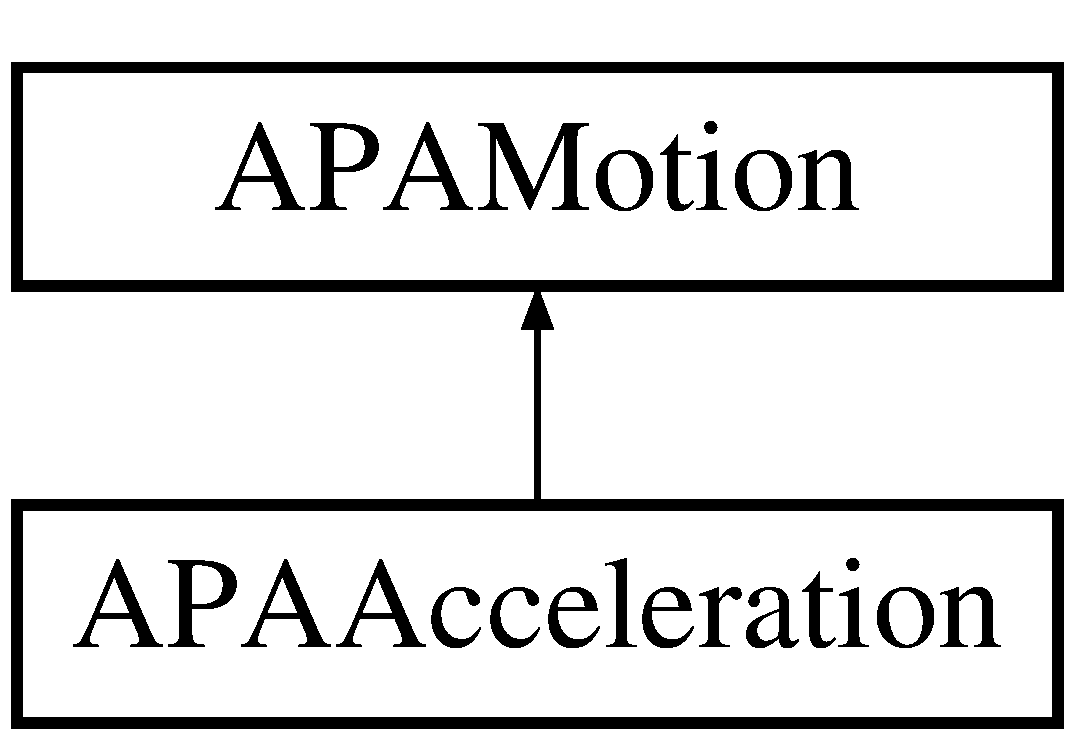
\includegraphics[height=2.000000cm]{class_a_p_a_acceleration}
\end{center}
\end{figure}
\subsection*{Public Member Functions}
\begin{DoxyCompactItemize}
\item 
\hyperlink{class_a_p_a_acceleration_a9236a1d22e7497197df8670fc47f70b6}{A\+P\+A\+Acceleration} ()
\item 
\hyperlink{class_a_p_a_acceleration_a962402484067c595d6e4c8e1efed1f1f}{$\sim$\+A\+P\+A\+Acceleration} ()
\item 
void \hyperlink{class_a_p_a_acceleration_a02e69859d063f4c7c94fe429549da92e}{accelerometer\+Changed} (float x, float y, float z) override
\item 
void \hyperlink{class_a_p_a_acceleration_a6b09386fa27a86904279e4c4715b3b08}{gyrometer\+Changed} (float x, float y, float z) override
\item 
\hyperlink{struct_gyrometer_data}{Gyrometer\+Data} $\ast$ \hyperlink{class_a_p_a_acceleration_a116b61825f2266522cbd753e1243f8f7}{get\+Gyrometer\+Data} ()
\item 
\hyperlink{struct_accelerometer_data}{Accelerometer\+Data} $\ast$ \hyperlink{class_a_p_a_acceleration_acbdad2f91dbc8508050914748c07c9f4}{get\+Accelerometer\+Data} ()
\end{DoxyCompactItemize}


\subsection{Constructor \& Destructor Documentation}
\hypertarget{class_a_p_a_acceleration_a9236a1d22e7497197df8670fc47f70b6}{\index{A\+P\+A\+Acceleration@{A\+P\+A\+Acceleration}!A\+P\+A\+Acceleration@{A\+P\+A\+Acceleration}}
\index{A\+P\+A\+Acceleration@{A\+P\+A\+Acceleration}!A\+P\+A\+Acceleration@{A\+P\+A\+Acceleration}}
\subsubsection[{A\+P\+A\+Acceleration}]{\setlength{\rightskip}{0pt plus 5cm}A\+P\+A\+Acceleration\+::\+A\+P\+A\+Acceleration (
\begin{DoxyParamCaption}
{}
\end{DoxyParamCaption}
)}}\label{class_a_p_a_acceleration_a9236a1d22e7497197df8670fc47f70b6}
\hypertarget{class_a_p_a_acceleration_a962402484067c595d6e4c8e1efed1f1f}{\index{A\+P\+A\+Acceleration@{A\+P\+A\+Acceleration}!````~A\+P\+A\+Acceleration@{$\sim$\+A\+P\+A\+Acceleration}}
\index{````~A\+P\+A\+Acceleration@{$\sim$\+A\+P\+A\+Acceleration}!A\+P\+A\+Acceleration@{A\+P\+A\+Acceleration}}
\subsubsection[{$\sim$\+A\+P\+A\+Acceleration}]{\setlength{\rightskip}{0pt plus 5cm}A\+P\+A\+Acceleration\+::$\sim$\+A\+P\+A\+Acceleration (
\begin{DoxyParamCaption}
{}
\end{DoxyParamCaption}
)}}\label{class_a_p_a_acceleration_a962402484067c595d6e4c8e1efed1f1f}


\subsection{Member Function Documentation}
\hypertarget{class_a_p_a_acceleration_a02e69859d063f4c7c94fe429549da92e}{\index{A\+P\+A\+Acceleration@{A\+P\+A\+Acceleration}!accelerometer\+Changed@{accelerometer\+Changed}}
\index{accelerometer\+Changed@{accelerometer\+Changed}!A\+P\+A\+Acceleration@{A\+P\+A\+Acceleration}}
\subsubsection[{accelerometer\+Changed}]{\setlength{\rightskip}{0pt plus 5cm}void A\+P\+A\+Acceleration\+::accelerometer\+Changed (
\begin{DoxyParamCaption}
\item[{float}]{x, }
\item[{float}]{y, }
\item[{float}]{z}
\end{DoxyParamCaption}
)\hspace{0.3cm}{\ttfamily [override]}, {\ttfamily [virtual]}}}\label{class_a_p_a_acceleration_a02e69859d063f4c7c94fe429549da92e}


Implements \hyperlink{class_a_p_a_motion_a6d6cd5ac438aabf7a60a080c1632dc10}{A\+P\+A\+Motion}.

\hypertarget{class_a_p_a_acceleration_acbdad2f91dbc8508050914748c07c9f4}{\index{A\+P\+A\+Acceleration@{A\+P\+A\+Acceleration}!get\+Accelerometer\+Data@{get\+Accelerometer\+Data}}
\index{get\+Accelerometer\+Data@{get\+Accelerometer\+Data}!A\+P\+A\+Acceleration@{A\+P\+A\+Acceleration}}
\subsubsection[{get\+Accelerometer\+Data}]{\setlength{\rightskip}{0pt plus 5cm}{\bf Accelerometer\+Data}$\ast$ A\+P\+A\+Acceleration\+::get\+Accelerometer\+Data (
\begin{DoxyParamCaption}
{}
\end{DoxyParamCaption}
)\hspace{0.3cm}{\ttfamily [inline]}}}\label{class_a_p_a_acceleration_acbdad2f91dbc8508050914748c07c9f4}
\hypertarget{class_a_p_a_acceleration_a116b61825f2266522cbd753e1243f8f7}{\index{A\+P\+A\+Acceleration@{A\+P\+A\+Acceleration}!get\+Gyrometer\+Data@{get\+Gyrometer\+Data}}
\index{get\+Gyrometer\+Data@{get\+Gyrometer\+Data}!A\+P\+A\+Acceleration@{A\+P\+A\+Acceleration}}
\subsubsection[{get\+Gyrometer\+Data}]{\setlength{\rightskip}{0pt plus 5cm}{\bf Gyrometer\+Data}$\ast$ A\+P\+A\+Acceleration\+::get\+Gyrometer\+Data (
\begin{DoxyParamCaption}
{}
\end{DoxyParamCaption}
)\hspace{0.3cm}{\ttfamily [inline]}}}\label{class_a_p_a_acceleration_a116b61825f2266522cbd753e1243f8f7}
\hypertarget{class_a_p_a_acceleration_a6b09386fa27a86904279e4c4715b3b08}{\index{A\+P\+A\+Acceleration@{A\+P\+A\+Acceleration}!gyrometer\+Changed@{gyrometer\+Changed}}
\index{gyrometer\+Changed@{gyrometer\+Changed}!A\+P\+A\+Acceleration@{A\+P\+A\+Acceleration}}
\subsubsection[{gyrometer\+Changed}]{\setlength{\rightskip}{0pt plus 5cm}void A\+P\+A\+Acceleration\+::gyrometer\+Changed (
\begin{DoxyParamCaption}
\item[{float}]{x, }
\item[{float}]{y, }
\item[{float}]{z}
\end{DoxyParamCaption}
)\hspace{0.3cm}{\ttfamily [override]}, {\ttfamily [virtual]}}}\label{class_a_p_a_acceleration_a6b09386fa27a86904279e4c4715b3b08}


Implements \hyperlink{class_a_p_a_motion_a79ca82357e31f95ed8de484a6e3e3882}{A\+P\+A\+Motion}.



The documentation for this class was generated from the following file\+:\begin{DoxyCompactItemize}
\item 
i\+O\+S\+Sensor\+Wrappers/\+Headers/\hyperlink{_acceleration_8h}{Acceleration.\+h}\end{DoxyCompactItemize}

\hypertarget{class_a_p_a_event}{\section{A\+P\+A\+Event Class Reference}
\label{class_a_p_a_event}\index{A\+P\+A\+Event@{A\+P\+A\+Event}}
}


{\ttfamily \#include $<$A\+P\+A\+Event.\+h$>$}

\subsection*{Public Member Functions}
\begin{DoxyCompactItemize}
\item 
\hyperlink{class_a_p_a_event_ac92fedacd1abd64f91ae8bbd2e96511d}{A\+P\+A\+Event} ()
\item 
\hyperlink{class_a_p_a_event_a5721119a8c565ea8d2beafbe743dfd40}{A\+P\+A\+Event} (unsigned long int time\+Stamp, \hyperlink{_a_p_a_event_8h_a945143d383a512a7400032d931d687b8}{Event\+Function} function, bool repeat)
\item 
\hyperlink{class_a_p_a_event_ade25624573f8faa8ae98bc1930c83758}{$\sim$\+A\+P\+A\+Event} ()
\item 
unsigned long int \hyperlink{class_a_p_a_event_a63b921fe498910e2f8cdcd317db95cef}{get\+Time\+Stamp} ()
\item 
unsigned long int \hyperlink{class_a_p_a_event_aaaf9759c8a5bdb6cc5a1daca4dcf7b6f}{get\+Offset} ()
\item 
\hyperlink{_a_p_a_event_8h_a945143d383a512a7400032d931d687b8}{Event\+Function} \hyperlink{class_a_p_a_event_a328b925b682b9a2466d9f2f4b2cbbc44}{get\+Function} ()
\item 
bool \hyperlink{class_a_p_a_event_a1056010bb8759bf4184cf171c83079a8}{get\+Repeat} ()
\item 
void \hyperlink{class_a_p_a_event_a042047db43eb412b29a69ff9bbf0b3d0}{process} ()
\end{DoxyCompactItemize}


\subsection{Constructor \& Destructor Documentation}
\hypertarget{class_a_p_a_event_ac92fedacd1abd64f91ae8bbd2e96511d}{\index{A\+P\+A\+Event@{A\+P\+A\+Event}!A\+P\+A\+Event@{A\+P\+A\+Event}}
\index{A\+P\+A\+Event@{A\+P\+A\+Event}!A\+P\+A\+Event@{A\+P\+A\+Event}}
\subsubsection[{A\+P\+A\+Event}]{\setlength{\rightskip}{0pt plus 5cm}A\+P\+A\+Event\+::\+A\+P\+A\+Event (
\begin{DoxyParamCaption}
{}
\end{DoxyParamCaption}
)}}\label{class_a_p_a_event_ac92fedacd1abd64f91ae8bbd2e96511d}
\hypertarget{class_a_p_a_event_a5721119a8c565ea8d2beafbe743dfd40}{\index{A\+P\+A\+Event@{A\+P\+A\+Event}!A\+P\+A\+Event@{A\+P\+A\+Event}}
\index{A\+P\+A\+Event@{A\+P\+A\+Event}!A\+P\+A\+Event@{A\+P\+A\+Event}}
\subsubsection[{A\+P\+A\+Event}]{\setlength{\rightskip}{0pt plus 5cm}A\+P\+A\+Event\+::\+A\+P\+A\+Event (
\begin{DoxyParamCaption}
\item[{unsigned long int}]{time\+Stamp, }
\item[{{\bf Event\+Function}}]{function, }
\item[{bool}]{repeat}
\end{DoxyParamCaption}
)}}\label{class_a_p_a_event_a5721119a8c565ea8d2beafbe743dfd40}
\hypertarget{class_a_p_a_event_ade25624573f8faa8ae98bc1930c83758}{\index{A\+P\+A\+Event@{A\+P\+A\+Event}!````~A\+P\+A\+Event@{$\sim$\+A\+P\+A\+Event}}
\index{````~A\+P\+A\+Event@{$\sim$\+A\+P\+A\+Event}!A\+P\+A\+Event@{A\+P\+A\+Event}}
\subsubsection[{$\sim$\+A\+P\+A\+Event}]{\setlength{\rightskip}{0pt plus 5cm}A\+P\+A\+Event\+::$\sim$\+A\+P\+A\+Event (
\begin{DoxyParamCaption}
{}
\end{DoxyParamCaption}
)}}\label{class_a_p_a_event_ade25624573f8faa8ae98bc1930c83758}


\subsection{Member Function Documentation}
\hypertarget{class_a_p_a_event_a328b925b682b9a2466d9f2f4b2cbbc44}{\index{A\+P\+A\+Event@{A\+P\+A\+Event}!get\+Function@{get\+Function}}
\index{get\+Function@{get\+Function}!A\+P\+A\+Event@{A\+P\+A\+Event}}
\subsubsection[{get\+Function}]{\setlength{\rightskip}{0pt plus 5cm}{\bf Event\+Function} A\+P\+A\+Event\+::get\+Function (
\begin{DoxyParamCaption}
{}
\end{DoxyParamCaption}
)\hspace{0.3cm}{\ttfamily [inline]}}}\label{class_a_p_a_event_a328b925b682b9a2466d9f2f4b2cbbc44}
\hypertarget{class_a_p_a_event_aaaf9759c8a5bdb6cc5a1daca4dcf7b6f}{\index{A\+P\+A\+Event@{A\+P\+A\+Event}!get\+Offset@{get\+Offset}}
\index{get\+Offset@{get\+Offset}!A\+P\+A\+Event@{A\+P\+A\+Event}}
\subsubsection[{get\+Offset}]{\setlength{\rightskip}{0pt plus 5cm}unsigned long int A\+P\+A\+Event\+::get\+Offset (
\begin{DoxyParamCaption}
{}
\end{DoxyParamCaption}
)\hspace{0.3cm}{\ttfamily [inline]}}}\label{class_a_p_a_event_aaaf9759c8a5bdb6cc5a1daca4dcf7b6f}
\hypertarget{class_a_p_a_event_a1056010bb8759bf4184cf171c83079a8}{\index{A\+P\+A\+Event@{A\+P\+A\+Event}!get\+Repeat@{get\+Repeat}}
\index{get\+Repeat@{get\+Repeat}!A\+P\+A\+Event@{A\+P\+A\+Event}}
\subsubsection[{get\+Repeat}]{\setlength{\rightskip}{0pt plus 5cm}bool A\+P\+A\+Event\+::get\+Repeat (
\begin{DoxyParamCaption}
{}
\end{DoxyParamCaption}
)\hspace{0.3cm}{\ttfamily [inline]}}}\label{class_a_p_a_event_a1056010bb8759bf4184cf171c83079a8}
\hypertarget{class_a_p_a_event_a63b921fe498910e2f8cdcd317db95cef}{\index{A\+P\+A\+Event@{A\+P\+A\+Event}!get\+Time\+Stamp@{get\+Time\+Stamp}}
\index{get\+Time\+Stamp@{get\+Time\+Stamp}!A\+P\+A\+Event@{A\+P\+A\+Event}}
\subsubsection[{get\+Time\+Stamp}]{\setlength{\rightskip}{0pt plus 5cm}unsigned long int A\+P\+A\+Event\+::get\+Time\+Stamp (
\begin{DoxyParamCaption}
{}
\end{DoxyParamCaption}
)\hspace{0.3cm}{\ttfamily [inline]}}}\label{class_a_p_a_event_a63b921fe498910e2f8cdcd317db95cef}
\hypertarget{class_a_p_a_event_a042047db43eb412b29a69ff9bbf0b3d0}{\index{A\+P\+A\+Event@{A\+P\+A\+Event}!process@{process}}
\index{process@{process}!A\+P\+A\+Event@{A\+P\+A\+Event}}
\subsubsection[{process}]{\setlength{\rightskip}{0pt plus 5cm}void A\+P\+A\+Event\+::process (
\begin{DoxyParamCaption}
{}
\end{DoxyParamCaption}
)}}\label{class_a_p_a_event_a042047db43eb412b29a69ff9bbf0b3d0}


The documentation for this class was generated from the following files\+:\begin{DoxyCompactItemize}
\item 
Sequencer Classes/\+Headers/\hyperlink{_a_p_a_event_8h}{A\+P\+A\+Event.\+h}\item 
Sequencer Classes/\+Implementations/\hyperlink{_a_p_a_event_8cpp}{A\+P\+A\+Event.\+cpp}\end{DoxyCompactItemize}

\hypertarget{class_a_p_a_event_handler}{\section{A\+P\+A\+Event\+Handler Class Reference}
\label{class_a_p_a_event_handler}\index{A\+P\+A\+Event\+Handler@{A\+P\+A\+Event\+Handler}}
}


{\ttfamily \#include $<$A\+P\+A\+Event\+Handler.\+h$>$}

\subsection*{Public Member Functions}
\begin{DoxyCompactItemize}
\item 
\hyperlink{class_a_p_a_event_handler_a692104570353da0316de6806fd6b2d0c}{A\+P\+A\+Event\+Handler} ()
\item 
void \hyperlink{class_a_p_a_event_handler_a8f8ee34fb2fa3c7dc1a224ad0846a562}{add\+Human\+Event} (\hyperlink{class_a_p_a_event}{A\+P\+A\+Event} $\ast$event)
\item 
void \hyperlink{class_a_p_a_event_handler_acd88f7050282d0a3961625d9c1f5c0ee}{add\+Computer\+Event} (\hyperlink{class_a_p_a_event}{A\+P\+A\+Event} $\ast$event)
\end{DoxyCompactItemize}


\subsection{Constructor \& Destructor Documentation}
\hypertarget{class_a_p_a_event_handler_a692104570353da0316de6806fd6b2d0c}{\index{A\+P\+A\+Event\+Handler@{A\+P\+A\+Event\+Handler}!A\+P\+A\+Event\+Handler@{A\+P\+A\+Event\+Handler}}
\index{A\+P\+A\+Event\+Handler@{A\+P\+A\+Event\+Handler}!A\+P\+A\+Event\+Handler@{A\+P\+A\+Event\+Handler}}
\subsubsection[{A\+P\+A\+Event\+Handler}]{\setlength{\rightskip}{0pt plus 5cm}A\+P\+A\+Event\+Handler\+::\+A\+P\+A\+Event\+Handler (
\begin{DoxyParamCaption}
{}
\end{DoxyParamCaption}
)}}\label{class_a_p_a_event_handler_a692104570353da0316de6806fd6b2d0c}


\subsection{Member Function Documentation}
\hypertarget{class_a_p_a_event_handler_acd88f7050282d0a3961625d9c1f5c0ee}{\index{A\+P\+A\+Event\+Handler@{A\+P\+A\+Event\+Handler}!add\+Computer\+Event@{add\+Computer\+Event}}
\index{add\+Computer\+Event@{add\+Computer\+Event}!A\+P\+A\+Event\+Handler@{A\+P\+A\+Event\+Handler}}
\subsubsection[{add\+Computer\+Event}]{\setlength{\rightskip}{0pt plus 5cm}void A\+P\+A\+Event\+Handler\+::add\+Computer\+Event (
\begin{DoxyParamCaption}
\item[{{\bf A\+P\+A\+Event} $\ast$}]{event}
\end{DoxyParamCaption}
)}}\label{class_a_p_a_event_handler_acd88f7050282d0a3961625d9c1f5c0ee}
\hypertarget{class_a_p_a_event_handler_a8f8ee34fb2fa3c7dc1a224ad0846a562}{\index{A\+P\+A\+Event\+Handler@{A\+P\+A\+Event\+Handler}!add\+Human\+Event@{add\+Human\+Event}}
\index{add\+Human\+Event@{add\+Human\+Event}!A\+P\+A\+Event\+Handler@{A\+P\+A\+Event\+Handler}}
\subsubsection[{add\+Human\+Event}]{\setlength{\rightskip}{0pt plus 5cm}void A\+P\+A\+Event\+Handler\+::add\+Human\+Event (
\begin{DoxyParamCaption}
\item[{{\bf A\+P\+A\+Event} $\ast$}]{event}
\end{DoxyParamCaption}
)}}\label{class_a_p_a_event_handler_a8f8ee34fb2fa3c7dc1a224ad0846a562}


The documentation for this class was generated from the following files\+:\begin{DoxyCompactItemize}
\item 
Sequencer Classes/\+Headers/\hyperlink{_a_p_a_event_handler_8h}{A\+P\+A\+Event\+Handler.\+h}\item 
Sequencer Classes/\+Implementations/\hyperlink{_a_p_a_event_handler_8cpp}{A\+P\+A\+Event\+Handler.\+cpp}\end{DoxyCompactItemize}

\hypertarget{class_a_p_a_midi_data}{\section{A\+P\+A\+Midi\+Data Class Reference}
\label{class_a_p_a_midi_data}\index{A\+P\+A\+Midi\+Data@{A\+P\+A\+Midi\+Data}}
}


{\ttfamily \#include $<$A\+P\+A\+Midi\+Data.\+h$>$}

\subsection*{Public Types}
\begin{DoxyCompactItemize}
\item 
using \hyperlink{class_a_p_a_midi_data_a5d20f609cfadb2b081f81da61840a473}{notes} = std\+::vector$<$ int $>$
\end{DoxyCompactItemize}
\subsection*{Public Attributes}
\begin{DoxyCompactItemize}
\item 
String \hyperlink{class_a_p_a_midi_data_ae8027131ba55c8755f452ddff07fb614}{I\+D}
\item 
std\+::vector$<$ int $>$ \hyperlink{class_a_p_a_midi_data_a449871212e64922701a7ae9191e3a013}{intervals}
\item 
std\+::vector$<$ \hyperlink{class_a_p_a_midi_data_a5d20f609cfadb2b081f81da61840a473}{notes} $>$ \hyperlink{class_a_p_a_midi_data_a281995e0adb7efdd2df91deb7c327d57}{phrase\+Intervals}
\item 
std\+::vector$<$ \hyperlink{class_a_p_a_midi_data_a5d20f609cfadb2b081f81da61840a473}{notes} $>$ \hyperlink{class_a_p_a_midi_data_a8b8b037cc91565601098df0a432c7619}{measure\+Intervals}
\end{DoxyCompactItemize}


\subsection{Member Typedef Documentation}
\hypertarget{class_a_p_a_midi_data_a5d20f609cfadb2b081f81da61840a473}{\index{A\+P\+A\+Midi\+Data@{A\+P\+A\+Midi\+Data}!notes@{notes}}
\index{notes@{notes}!A\+P\+A\+Midi\+Data@{A\+P\+A\+Midi\+Data}}
\subsubsection[{notes}]{\setlength{\rightskip}{0pt plus 5cm}using {\bf A\+P\+A\+Midi\+Data\+::notes} =  std\+::vector$<$int$>$}}\label{class_a_p_a_midi_data_a5d20f609cfadb2b081f81da61840a473}


\subsection{Member Data Documentation}
\hypertarget{class_a_p_a_midi_data_ae8027131ba55c8755f452ddff07fb614}{\index{A\+P\+A\+Midi\+Data@{A\+P\+A\+Midi\+Data}!I\+D@{I\+D}}
\index{I\+D@{I\+D}!A\+P\+A\+Midi\+Data@{A\+P\+A\+Midi\+Data}}
\subsubsection[{I\+D}]{\setlength{\rightskip}{0pt plus 5cm}String A\+P\+A\+Midi\+Data\+::\+I\+D}}\label{class_a_p_a_midi_data_ae8027131ba55c8755f452ddff07fb614}
\hypertarget{class_a_p_a_midi_data_a449871212e64922701a7ae9191e3a013}{\index{A\+P\+A\+Midi\+Data@{A\+P\+A\+Midi\+Data}!intervals@{intervals}}
\index{intervals@{intervals}!A\+P\+A\+Midi\+Data@{A\+P\+A\+Midi\+Data}}
\subsubsection[{intervals}]{\setlength{\rightskip}{0pt plus 5cm}std\+::vector$<$int$>$ A\+P\+A\+Midi\+Data\+::intervals}}\label{class_a_p_a_midi_data_a449871212e64922701a7ae9191e3a013}
\hypertarget{class_a_p_a_midi_data_a8b8b037cc91565601098df0a432c7619}{\index{A\+P\+A\+Midi\+Data@{A\+P\+A\+Midi\+Data}!measure\+Intervals@{measure\+Intervals}}
\index{measure\+Intervals@{measure\+Intervals}!A\+P\+A\+Midi\+Data@{A\+P\+A\+Midi\+Data}}
\subsubsection[{measure\+Intervals}]{\setlength{\rightskip}{0pt plus 5cm}std\+::vector$<${\bf notes}$>$ A\+P\+A\+Midi\+Data\+::measure\+Intervals}}\label{class_a_p_a_midi_data_a8b8b037cc91565601098df0a432c7619}
\hypertarget{class_a_p_a_midi_data_a281995e0adb7efdd2df91deb7c327d57}{\index{A\+P\+A\+Midi\+Data@{A\+P\+A\+Midi\+Data}!phrase\+Intervals@{phrase\+Intervals}}
\index{phrase\+Intervals@{phrase\+Intervals}!A\+P\+A\+Midi\+Data@{A\+P\+A\+Midi\+Data}}
\subsubsection[{phrase\+Intervals}]{\setlength{\rightskip}{0pt plus 5cm}std\+::vector$<${\bf notes}$>$ A\+P\+A\+Midi\+Data\+::phrase\+Intervals}}\label{class_a_p_a_midi_data_a281995e0adb7efdd2df91deb7c327d57}


The documentation for this class was generated from the following file\+:\begin{DoxyCompactItemize}
\item 
Midi Classes/\+Headers/\hyperlink{_a_p_a_midi_data_8h}{A\+P\+A\+Midi\+Data.\+h}\end{DoxyCompactItemize}

\hypertarget{class_a_p_a_midi_database}{\section{A\+P\+A\+Midi\+Database Class Reference}
\label{class_a_p_a_midi_database}\index{A\+P\+A\+Midi\+Database@{A\+P\+A\+Midi\+Database}}
}


{\ttfamily \#include $<$A\+P\+A\+Midi\+Database.\+h$>$}

\subsection*{Public Member Functions}
\begin{DoxyCompactItemize}
\item 
\hyperlink{class_a_p_a_midi_database_a74c56afddf6b0dd53727b64cdd407cbe}{A\+P\+A\+Midi\+Database} ()
\item 
\hyperlink{class_a_p_a_midi_database_abc39fdf72bb5abd3743041b92b2566ea}{$\sim$\+A\+P\+A\+Midi\+Database} ()
\item 
void \hyperlink{class_a_p_a_midi_database_a6318128aaa8d714ebbb4831477e1b92f}{load} ()
\item 
void \hyperlink{class_a_p_a_midi_database_a2f442d74f42dfd128b1af1ae4efeefbf}{load\+Composition} ()
\item 
\hyperlink{class_a_p_a_midi_data}{A\+P\+A\+Midi\+Data} \hyperlink{class_a_p_a_midi_database_a047f8526f4910efc4e39c309f216bb9d}{get\+Data} ()
\end{DoxyCompactItemize}


\subsection{Constructor \& Destructor Documentation}
\hypertarget{class_a_p_a_midi_database_a74c56afddf6b0dd53727b64cdd407cbe}{\index{A\+P\+A\+Midi\+Database@{A\+P\+A\+Midi\+Database}!A\+P\+A\+Midi\+Database@{A\+P\+A\+Midi\+Database}}
\index{A\+P\+A\+Midi\+Database@{A\+P\+A\+Midi\+Database}!A\+P\+A\+Midi\+Database@{A\+P\+A\+Midi\+Database}}
\subsubsection[{A\+P\+A\+Midi\+Database}]{\setlength{\rightskip}{0pt plus 5cm}A\+P\+A\+Midi\+Database\+::\+A\+P\+A\+Midi\+Database (
\begin{DoxyParamCaption}
{}
\end{DoxyParamCaption}
)}}\label{class_a_p_a_midi_database_a74c56afddf6b0dd53727b64cdd407cbe}
\hypertarget{class_a_p_a_midi_database_abc39fdf72bb5abd3743041b92b2566ea}{\index{A\+P\+A\+Midi\+Database@{A\+P\+A\+Midi\+Database}!````~A\+P\+A\+Midi\+Database@{$\sim$\+A\+P\+A\+Midi\+Database}}
\index{````~A\+P\+A\+Midi\+Database@{$\sim$\+A\+P\+A\+Midi\+Database}!A\+P\+A\+Midi\+Database@{A\+P\+A\+Midi\+Database}}
\subsubsection[{$\sim$\+A\+P\+A\+Midi\+Database}]{\setlength{\rightskip}{0pt plus 5cm}A\+P\+A\+Midi\+Database\+::$\sim$\+A\+P\+A\+Midi\+Database (
\begin{DoxyParamCaption}
{}
\end{DoxyParamCaption}
)}}\label{class_a_p_a_midi_database_abc39fdf72bb5abd3743041b92b2566ea}


\subsection{Member Function Documentation}
\hypertarget{class_a_p_a_midi_database_a047f8526f4910efc4e39c309f216bb9d}{\index{A\+P\+A\+Midi\+Database@{A\+P\+A\+Midi\+Database}!get\+Data@{get\+Data}}
\index{get\+Data@{get\+Data}!A\+P\+A\+Midi\+Database@{A\+P\+A\+Midi\+Database}}
\subsubsection[{get\+Data}]{\setlength{\rightskip}{0pt plus 5cm}{\bf A\+P\+A\+Midi\+Data} A\+P\+A\+Midi\+Database\+::get\+Data (
\begin{DoxyParamCaption}
{}
\end{DoxyParamCaption}
)\hspace{0.3cm}{\ttfamily [inline]}}}\label{class_a_p_a_midi_database_a047f8526f4910efc4e39c309f216bb9d}
\hypertarget{class_a_p_a_midi_database_a6318128aaa8d714ebbb4831477e1b92f}{\index{A\+P\+A\+Midi\+Database@{A\+P\+A\+Midi\+Database}!load@{load}}
\index{load@{load}!A\+P\+A\+Midi\+Database@{A\+P\+A\+Midi\+Database}}
\subsubsection[{load}]{\setlength{\rightskip}{0pt plus 5cm}void A\+P\+A\+Midi\+Database\+::load (
\begin{DoxyParamCaption}
{}
\end{DoxyParamCaption}
)}}\label{class_a_p_a_midi_database_a6318128aaa8d714ebbb4831477e1b92f}
\hypertarget{class_a_p_a_midi_database_a2f442d74f42dfd128b1af1ae4efeefbf}{\index{A\+P\+A\+Midi\+Database@{A\+P\+A\+Midi\+Database}!load\+Composition@{load\+Composition}}
\index{load\+Composition@{load\+Composition}!A\+P\+A\+Midi\+Database@{A\+P\+A\+Midi\+Database}}
\subsubsection[{load\+Composition}]{\setlength{\rightskip}{0pt plus 5cm}void A\+P\+A\+Midi\+Database\+::load\+Composition (
\begin{DoxyParamCaption}
{}
\end{DoxyParamCaption}
)}}\label{class_a_p_a_midi_database_a2f442d74f42dfd128b1af1ae4efeefbf}


The documentation for this class was generated from the following files\+:\begin{DoxyCompactItemize}
\item 
Midi Classes/\+Headers/\hyperlink{_a_p_a_midi_database_8h}{A\+P\+A\+Midi\+Database.\+h}\item 
Midi Classes/\+Implementations/\hyperlink{_a_p_a_midi_database_8cpp}{A\+P\+A\+Midi\+Database.\+cpp}\end{DoxyCompactItemize}

\hypertarget{class_a_p_a_midi_loader}{\section{A\+P\+A\+Midi\+Loader Class Reference}
\label{class_a_p_a_midi_loader}\index{A\+P\+A\+Midi\+Loader@{A\+P\+A\+Midi\+Loader}}
}


{\ttfamily \#include $<$A\+P\+A\+Midi\+Loader.\+h$>$}

\subsection*{Public Member Functions}
\begin{DoxyCompactItemize}
\item 
\hyperlink{class_a_p_a_midi_loader_a62e4870f73cc32fdb84f23c7be88c2bb}{A\+P\+A\+Midi\+Loader} ()
\item 
\hyperlink{class_a_p_a_midi_loader_a25c40f24ab01b8797a0f438d9f90cd52}{A\+P\+A\+Midi\+Loader} (unsigned int measure\+Size, unsigned int phrase\+Size)
\item 
void \hyperlink{class_a_p_a_midi_loader_a6b9dfe9c5602d4eab720cc468c90ebaa}{set\+Measure\+Size} (unsigned int measure\+Size)
\item 
void \hyperlink{class_a_p_a_midi_loader_a137cdb38017629f07c802ea8a0c9615b}{set\+Phrase\+Size} (unsigned int phrase\+Size)
\item 
\hyperlink{class_a_p_a_midi_data}{A\+P\+A\+Midi\+Data} \hyperlink{class_a_p_a_midi_loader_ad08cb2ad3a616c4e9c3cafd4bf5a6f90}{load\+Data} (File data\+File)
\end{DoxyCompactItemize}


\subsection{Constructor \& Destructor Documentation}
\hypertarget{class_a_p_a_midi_loader_a62e4870f73cc32fdb84f23c7be88c2bb}{\index{A\+P\+A\+Midi\+Loader@{A\+P\+A\+Midi\+Loader}!A\+P\+A\+Midi\+Loader@{A\+P\+A\+Midi\+Loader}}
\index{A\+P\+A\+Midi\+Loader@{A\+P\+A\+Midi\+Loader}!A\+P\+A\+Midi\+Loader@{A\+P\+A\+Midi\+Loader}}
\subsubsection[{A\+P\+A\+Midi\+Loader}]{\setlength{\rightskip}{0pt plus 5cm}A\+P\+A\+Midi\+Loader\+::\+A\+P\+A\+Midi\+Loader (
\begin{DoxyParamCaption}
{}
\end{DoxyParamCaption}
)}}\label{class_a_p_a_midi_loader_a62e4870f73cc32fdb84f23c7be88c2bb}
\hypertarget{class_a_p_a_midi_loader_a25c40f24ab01b8797a0f438d9f90cd52}{\index{A\+P\+A\+Midi\+Loader@{A\+P\+A\+Midi\+Loader}!A\+P\+A\+Midi\+Loader@{A\+P\+A\+Midi\+Loader}}
\index{A\+P\+A\+Midi\+Loader@{A\+P\+A\+Midi\+Loader}!A\+P\+A\+Midi\+Loader@{A\+P\+A\+Midi\+Loader}}
\subsubsection[{A\+P\+A\+Midi\+Loader}]{\setlength{\rightskip}{0pt plus 5cm}A\+P\+A\+Midi\+Loader\+::\+A\+P\+A\+Midi\+Loader (
\begin{DoxyParamCaption}
\item[{unsigned int}]{measure\+Size, }
\item[{unsigned int}]{phrase\+Size}
\end{DoxyParamCaption}
)}}\label{class_a_p_a_midi_loader_a25c40f24ab01b8797a0f438d9f90cd52}


\subsection{Member Function Documentation}
\hypertarget{class_a_p_a_midi_loader_ad08cb2ad3a616c4e9c3cafd4bf5a6f90}{\index{A\+P\+A\+Midi\+Loader@{A\+P\+A\+Midi\+Loader}!load\+Data@{load\+Data}}
\index{load\+Data@{load\+Data}!A\+P\+A\+Midi\+Loader@{A\+P\+A\+Midi\+Loader}}
\subsubsection[{load\+Data}]{\setlength{\rightskip}{0pt plus 5cm}{\bf A\+P\+A\+Midi\+Data} A\+P\+A\+Midi\+Loader\+::load\+Data (
\begin{DoxyParamCaption}
\item[{File}]{data\+File}
\end{DoxyParamCaption}
)}}\label{class_a_p_a_midi_loader_ad08cb2ad3a616c4e9c3cafd4bf5a6f90}
\hypertarget{class_a_p_a_midi_loader_a6b9dfe9c5602d4eab720cc468c90ebaa}{\index{A\+P\+A\+Midi\+Loader@{A\+P\+A\+Midi\+Loader}!set\+Measure\+Size@{set\+Measure\+Size}}
\index{set\+Measure\+Size@{set\+Measure\+Size}!A\+P\+A\+Midi\+Loader@{A\+P\+A\+Midi\+Loader}}
\subsubsection[{set\+Measure\+Size}]{\setlength{\rightskip}{0pt plus 5cm}void A\+P\+A\+Midi\+Loader\+::set\+Measure\+Size (
\begin{DoxyParamCaption}
\item[{unsigned int}]{measure\+Size}
\end{DoxyParamCaption}
)}}\label{class_a_p_a_midi_loader_a6b9dfe9c5602d4eab720cc468c90ebaa}
\hypertarget{class_a_p_a_midi_loader_a137cdb38017629f07c802ea8a0c9615b}{\index{A\+P\+A\+Midi\+Loader@{A\+P\+A\+Midi\+Loader}!set\+Phrase\+Size@{set\+Phrase\+Size}}
\index{set\+Phrase\+Size@{set\+Phrase\+Size}!A\+P\+A\+Midi\+Loader@{A\+P\+A\+Midi\+Loader}}
\subsubsection[{set\+Phrase\+Size}]{\setlength{\rightskip}{0pt plus 5cm}void A\+P\+A\+Midi\+Loader\+::set\+Phrase\+Size (
\begin{DoxyParamCaption}
\item[{unsigned int}]{phrase\+Size}
\end{DoxyParamCaption}
)}}\label{class_a_p_a_midi_loader_a137cdb38017629f07c802ea8a0c9615b}


The documentation for this class was generated from the following files\+:\begin{DoxyCompactItemize}
\item 
Midi Classes/\+Headers/\hyperlink{_a_p_a_midi_loader_8h}{A\+P\+A\+Midi\+Loader.\+h}\item 
Midi Classes/\+Implementations/\hyperlink{_a_p_a_midi_loader_8cpp}{A\+P\+A\+Midi\+Loader.\+cpp}\end{DoxyCompactItemize}

\hypertarget{class_a_p_a_motion}{\section{A\+P\+A\+Motion Class Reference}
\label{class_a_p_a_motion}\index{A\+P\+A\+Motion@{A\+P\+A\+Motion}}
}


{\ttfamily \#include $<$Motion.\+h$>$}

Inheritance diagram for A\+P\+A\+Motion\+:\begin{figure}[H]
\begin{center}
\leavevmode
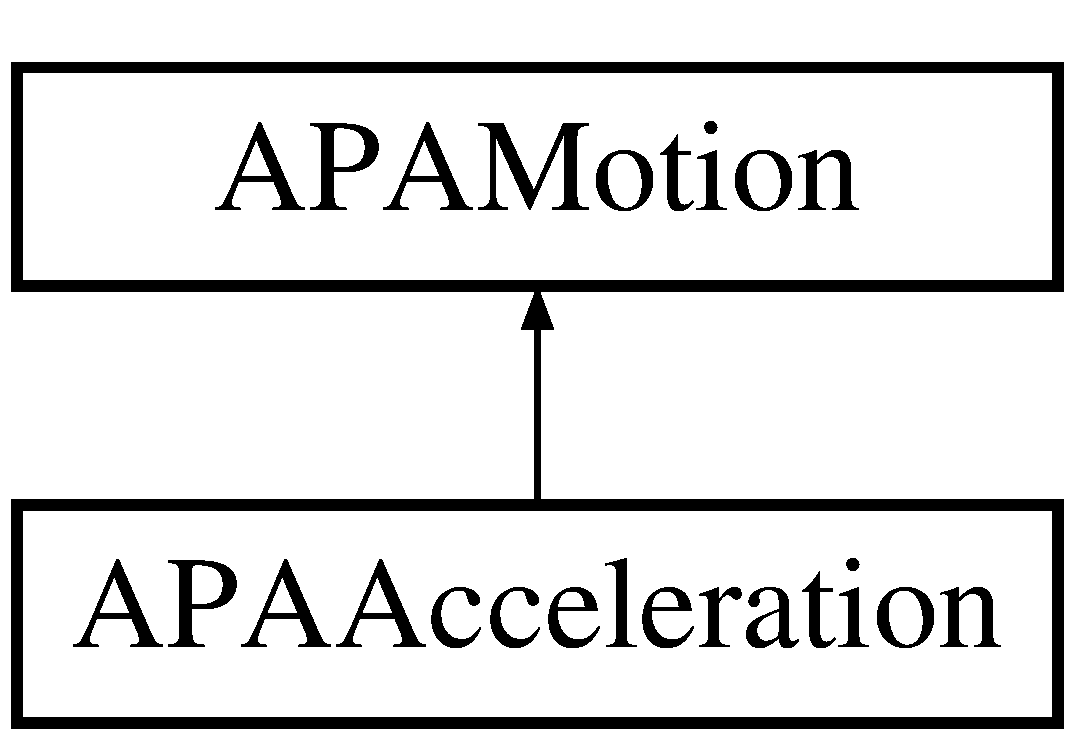
\includegraphics[height=2.000000cm]{class_a_p_a_motion}
\end{center}
\end{figure}
\subsection*{Public Member Functions}
\begin{DoxyCompactItemize}
\item 
\hyperlink{class_a_p_a_motion_a929c72a677d5543b0cf2a19707a9e163}{A\+P\+A\+Motion} ()
\item 
virtual \hyperlink{class_a_p_a_motion_ae074f8b140ce4fe8febbe695f07c015d}{$\sim$\+A\+P\+A\+Motion} ()
\item 
virtual void \hyperlink{class_a_p_a_motion_a6d6cd5ac438aabf7a60a080c1632dc10}{accelerometer\+Changed} (float x, float y, float z)=0
\item 
virtual void \hyperlink{class_a_p_a_motion_a79ca82357e31f95ed8de484a6e3e3882}{gyrometer\+Changed} (float x, float y, float z)=0
\end{DoxyCompactItemize}


\subsection{Constructor \& Destructor Documentation}
\hypertarget{class_a_p_a_motion_a929c72a677d5543b0cf2a19707a9e163}{\index{A\+P\+A\+Motion@{A\+P\+A\+Motion}!A\+P\+A\+Motion@{A\+P\+A\+Motion}}
\index{A\+P\+A\+Motion@{A\+P\+A\+Motion}!A\+P\+A\+Motion@{A\+P\+A\+Motion}}
\subsubsection[{A\+P\+A\+Motion}]{\setlength{\rightskip}{0pt plus 5cm}A\+P\+A\+Motion\+::\+A\+P\+A\+Motion (
\begin{DoxyParamCaption}
{}
\end{DoxyParamCaption}
)}}\label{class_a_p_a_motion_a929c72a677d5543b0cf2a19707a9e163}
\hypertarget{class_a_p_a_motion_ae074f8b140ce4fe8febbe695f07c015d}{\index{A\+P\+A\+Motion@{A\+P\+A\+Motion}!````~A\+P\+A\+Motion@{$\sim$\+A\+P\+A\+Motion}}
\index{````~A\+P\+A\+Motion@{$\sim$\+A\+P\+A\+Motion}!A\+P\+A\+Motion@{A\+P\+A\+Motion}}
\subsubsection[{$\sim$\+A\+P\+A\+Motion}]{\setlength{\rightskip}{0pt plus 5cm}virtual A\+P\+A\+Motion\+::$\sim$\+A\+P\+A\+Motion (
\begin{DoxyParamCaption}
{}
\end{DoxyParamCaption}
)\hspace{0.3cm}{\ttfamily [virtual]}}}\label{class_a_p_a_motion_ae074f8b140ce4fe8febbe695f07c015d}


\subsection{Member Function Documentation}
\hypertarget{class_a_p_a_motion_a6d6cd5ac438aabf7a60a080c1632dc10}{\index{A\+P\+A\+Motion@{A\+P\+A\+Motion}!accelerometer\+Changed@{accelerometer\+Changed}}
\index{accelerometer\+Changed@{accelerometer\+Changed}!A\+P\+A\+Motion@{A\+P\+A\+Motion}}
\subsubsection[{accelerometer\+Changed}]{\setlength{\rightskip}{0pt plus 5cm}virtual void A\+P\+A\+Motion\+::accelerometer\+Changed (
\begin{DoxyParamCaption}
\item[{float}]{x, }
\item[{float}]{y, }
\item[{float}]{z}
\end{DoxyParamCaption}
)\hspace{0.3cm}{\ttfamily [pure virtual]}}}\label{class_a_p_a_motion_a6d6cd5ac438aabf7a60a080c1632dc10}


Implemented in \hyperlink{class_a_p_a_acceleration_a02e69859d063f4c7c94fe429549da92e}{A\+P\+A\+Acceleration}.

\hypertarget{class_a_p_a_motion_a79ca82357e31f95ed8de484a6e3e3882}{\index{A\+P\+A\+Motion@{A\+P\+A\+Motion}!gyrometer\+Changed@{gyrometer\+Changed}}
\index{gyrometer\+Changed@{gyrometer\+Changed}!A\+P\+A\+Motion@{A\+P\+A\+Motion}}
\subsubsection[{gyrometer\+Changed}]{\setlength{\rightskip}{0pt plus 5cm}virtual void A\+P\+A\+Motion\+::gyrometer\+Changed (
\begin{DoxyParamCaption}
\item[{float}]{x, }
\item[{float}]{y, }
\item[{float}]{z}
\end{DoxyParamCaption}
)\hspace{0.3cm}{\ttfamily [pure virtual]}}}\label{class_a_p_a_motion_a79ca82357e31f95ed8de484a6e3e3882}


Implemented in \hyperlink{class_a_p_a_acceleration_a6b09386fa27a86904279e4c4715b3b08}{A\+P\+A\+Acceleration}.



The documentation for this class was generated from the following file\+:\begin{DoxyCompactItemize}
\item 
i\+O\+S\+Sensor\+Wrappers/\+Headers/\hyperlink{_motion_8h}{Motion.\+h}\end{DoxyCompactItemize}

\hypertarget{class_a_p_a_music_parser}{\section{A\+P\+A\+Music\+Parser Class Reference}
\label{class_a_p_a_music_parser}\index{A\+P\+A\+Music\+Parser@{A\+P\+A\+Music\+Parser}}
}


{\ttfamily \#include $<$A\+P\+A\+Music\+Parser.\+h$>$}

\subsection*{Public Member Functions}
\begin{DoxyCompactItemize}
\item 
\hyperlink{class_a_p_a_music_parser_a96224ba6553496fd6a9c3e189984e763}{A\+P\+A\+Music\+Parser} ()
\item 
\hyperlink{class_a_p_a_music_parser_a40dbb74982bbd0098125cf5810fa90f5}{$\sim$\+A\+P\+A\+Music\+Parser} ()
\item 
void \hyperlink{class_a_p_a_music_parser_a0ba4b420cc21f29a754bb8729c4d14b7}{load\+Music\+File} ()
\item 
void \hyperlink{class_a_p_a_music_parser_afb852353adf6e400f2a917ea72910099}{check\+For\+Events} ()
\end{DoxyCompactItemize}


\subsection{Constructor \& Destructor Documentation}
\hypertarget{class_a_p_a_music_parser_a96224ba6553496fd6a9c3e189984e763}{\index{A\+P\+A\+Music\+Parser@{A\+P\+A\+Music\+Parser}!A\+P\+A\+Music\+Parser@{A\+P\+A\+Music\+Parser}}
\index{A\+P\+A\+Music\+Parser@{A\+P\+A\+Music\+Parser}!A\+P\+A\+Music\+Parser@{A\+P\+A\+Music\+Parser}}
\subsubsection[{A\+P\+A\+Music\+Parser}]{\setlength{\rightskip}{0pt plus 5cm}A\+P\+A\+Music\+Parser\+::\+A\+P\+A\+Music\+Parser (
\begin{DoxyParamCaption}
{}
\end{DoxyParamCaption}
)}}\label{class_a_p_a_music_parser_a96224ba6553496fd6a9c3e189984e763}
\hypertarget{class_a_p_a_music_parser_a40dbb74982bbd0098125cf5810fa90f5}{\index{A\+P\+A\+Music\+Parser@{A\+P\+A\+Music\+Parser}!````~A\+P\+A\+Music\+Parser@{$\sim$\+A\+P\+A\+Music\+Parser}}
\index{````~A\+P\+A\+Music\+Parser@{$\sim$\+A\+P\+A\+Music\+Parser}!A\+P\+A\+Music\+Parser@{A\+P\+A\+Music\+Parser}}
\subsubsection[{$\sim$\+A\+P\+A\+Music\+Parser}]{\setlength{\rightskip}{0pt plus 5cm}A\+P\+A\+Music\+Parser\+::$\sim$\+A\+P\+A\+Music\+Parser (
\begin{DoxyParamCaption}
{}
\end{DoxyParamCaption}
)}}\label{class_a_p_a_music_parser_a40dbb74982bbd0098125cf5810fa90f5}


\subsection{Member Function Documentation}
\hypertarget{class_a_p_a_music_parser_afb852353adf6e400f2a917ea72910099}{\index{A\+P\+A\+Music\+Parser@{A\+P\+A\+Music\+Parser}!check\+For\+Events@{check\+For\+Events}}
\index{check\+For\+Events@{check\+For\+Events}!A\+P\+A\+Music\+Parser@{A\+P\+A\+Music\+Parser}}
\subsubsection[{check\+For\+Events}]{\setlength{\rightskip}{0pt plus 5cm}void A\+P\+A\+Music\+Parser\+::check\+For\+Events (
\begin{DoxyParamCaption}
{}
\end{DoxyParamCaption}
)}}\label{class_a_p_a_music_parser_afb852353adf6e400f2a917ea72910099}
\hypertarget{class_a_p_a_music_parser_a0ba4b420cc21f29a754bb8729c4d14b7}{\index{A\+P\+A\+Music\+Parser@{A\+P\+A\+Music\+Parser}!load\+Music\+File@{load\+Music\+File}}
\index{load\+Music\+File@{load\+Music\+File}!A\+P\+A\+Music\+Parser@{A\+P\+A\+Music\+Parser}}
\subsubsection[{load\+Music\+File}]{\setlength{\rightskip}{0pt plus 5cm}void A\+P\+A\+Music\+Parser\+::load\+Music\+File (
\begin{DoxyParamCaption}
{}
\end{DoxyParamCaption}
)}}\label{class_a_p_a_music_parser_a0ba4b420cc21f29a754bb8729c4d14b7}


The documentation for this class was generated from the following files\+:\begin{DoxyCompactItemize}
\item 
Music\+X\+M\+L Classes/\hyperlink{_a_p_a_music_parser_8h}{A\+P\+A\+Music\+Parser.\+h}\item 
Music\+X\+M\+L Classes/\hyperlink{_a_p_a_music_parser_8cpp}{A\+P\+A\+Music\+Parser.\+cpp}\end{DoxyCompactItemize}

\hypertarget{class_a_p_a_scheduler}{\section{A\+P\+A\+Scheduler Class Reference}
\label{class_a_p_a_scheduler}\index{A\+P\+A\+Scheduler@{A\+P\+A\+Scheduler}}
}


{\ttfamily \#include $<$A\+P\+A\+Scheduler.\+h$>$}

\subsection*{Public Types}
\begin{DoxyCompactItemize}
\item 
using \hyperlink{class_a_p_a_scheduler_a51416792b9612857bf15bd1452f822e5}{Event\+Funtion} = std\+::function$<$ void()$>$
\end{DoxyCompactItemize}
\subsection*{Public Member Functions}
\begin{DoxyCompactItemize}
\item 
\hyperlink{class_a_p_a_scheduler_a606aca3e9180d776ecd62cc3454c5c17}{A\+P\+A\+Scheduler} ()
\item 
\hyperlink{class_a_p_a_scheduler_ad9929c81e793d38ad0d55b34af6f6ba5}{$\sim$\+A\+P\+A\+Scheduler} ()
\item 
void \hyperlink{class_a_p_a_scheduler_a0553ca2cf524a6ad833568bbdb204558}{add\+Event} (unsigned long int time\+Stamp, \hyperlink{class_a_p_a_scheduler_a51416792b9612857bf15bd1452f822e5}{Event\+Funtion} function, bool repeat)
\item 
void \hyperlink{class_a_p_a_scheduler_afe745232bb05ab60f69a05c9e72f6f5b}{update} (unsigned long int time\+Stamp)
\item 
void \hyperlink{class_a_p_a_scheduler_a56a89836651d889fd91e4b8f4a84318b}{play} ()
\item 
void \hyperlink{class_a_p_a_scheduler_a568323cec2e3bf967648815ca39c130f}{stop} ()
\item 
unsigned long int \hyperlink{class_a_p_a_scheduler_a541c53fb4eb562029cb05a18de3fe9c2}{get\+Gurrent\+Time} ()
\end{DoxyCompactItemize}


\subsection{Member Typedef Documentation}
\hypertarget{class_a_p_a_scheduler_a51416792b9612857bf15bd1452f822e5}{\index{A\+P\+A\+Scheduler@{A\+P\+A\+Scheduler}!Event\+Funtion@{Event\+Funtion}}
\index{Event\+Funtion@{Event\+Funtion}!A\+P\+A\+Scheduler@{A\+P\+A\+Scheduler}}
\subsubsection[{Event\+Funtion}]{\setlength{\rightskip}{0pt plus 5cm}using {\bf A\+P\+A\+Scheduler\+::\+Event\+Funtion} =  std\+::function$<$void()$>$}}\label{class_a_p_a_scheduler_a51416792b9612857bf15bd1452f822e5}


\subsection{Constructor \& Destructor Documentation}
\hypertarget{class_a_p_a_scheduler_a606aca3e9180d776ecd62cc3454c5c17}{\index{A\+P\+A\+Scheduler@{A\+P\+A\+Scheduler}!A\+P\+A\+Scheduler@{A\+P\+A\+Scheduler}}
\index{A\+P\+A\+Scheduler@{A\+P\+A\+Scheduler}!A\+P\+A\+Scheduler@{A\+P\+A\+Scheduler}}
\subsubsection[{A\+P\+A\+Scheduler}]{\setlength{\rightskip}{0pt plus 5cm}A\+P\+A\+Scheduler\+::\+A\+P\+A\+Scheduler (
\begin{DoxyParamCaption}
{}
\end{DoxyParamCaption}
)}}\label{class_a_p_a_scheduler_a606aca3e9180d776ecd62cc3454c5c17}
\hypertarget{class_a_p_a_scheduler_ad9929c81e793d38ad0d55b34af6f6ba5}{\index{A\+P\+A\+Scheduler@{A\+P\+A\+Scheduler}!````~A\+P\+A\+Scheduler@{$\sim$\+A\+P\+A\+Scheduler}}
\index{````~A\+P\+A\+Scheduler@{$\sim$\+A\+P\+A\+Scheduler}!A\+P\+A\+Scheduler@{A\+P\+A\+Scheduler}}
\subsubsection[{$\sim$\+A\+P\+A\+Scheduler}]{\setlength{\rightskip}{0pt plus 5cm}A\+P\+A\+Scheduler\+::$\sim$\+A\+P\+A\+Scheduler (
\begin{DoxyParamCaption}
{}
\end{DoxyParamCaption}
)}}\label{class_a_p_a_scheduler_ad9929c81e793d38ad0d55b34af6f6ba5}


\subsection{Member Function Documentation}
\hypertarget{class_a_p_a_scheduler_a0553ca2cf524a6ad833568bbdb204558}{\index{A\+P\+A\+Scheduler@{A\+P\+A\+Scheduler}!add\+Event@{add\+Event}}
\index{add\+Event@{add\+Event}!A\+P\+A\+Scheduler@{A\+P\+A\+Scheduler}}
\subsubsection[{add\+Event}]{\setlength{\rightskip}{0pt plus 5cm}void A\+P\+A\+Scheduler\+::add\+Event (
\begin{DoxyParamCaption}
\item[{unsigned long int}]{time\+Stamp, }
\item[{{\bf Event\+Funtion}}]{function, }
\item[{bool}]{repeat}
\end{DoxyParamCaption}
)}}\label{class_a_p_a_scheduler_a0553ca2cf524a6ad833568bbdb204558}
\hypertarget{class_a_p_a_scheduler_a541c53fb4eb562029cb05a18de3fe9c2}{\index{A\+P\+A\+Scheduler@{A\+P\+A\+Scheduler}!get\+Gurrent\+Time@{get\+Gurrent\+Time}}
\index{get\+Gurrent\+Time@{get\+Gurrent\+Time}!A\+P\+A\+Scheduler@{A\+P\+A\+Scheduler}}
\subsubsection[{get\+Gurrent\+Time}]{\setlength{\rightskip}{0pt plus 5cm}unsigned long int A\+P\+A\+Scheduler\+::get\+Gurrent\+Time (
\begin{DoxyParamCaption}
{}
\end{DoxyParamCaption}
)\hspace{0.3cm}{\ttfamily [inline]}}}\label{class_a_p_a_scheduler_a541c53fb4eb562029cb05a18de3fe9c2}
\hypertarget{class_a_p_a_scheduler_a56a89836651d889fd91e4b8f4a84318b}{\index{A\+P\+A\+Scheduler@{A\+P\+A\+Scheduler}!play@{play}}
\index{play@{play}!A\+P\+A\+Scheduler@{A\+P\+A\+Scheduler}}
\subsubsection[{play}]{\setlength{\rightskip}{0pt plus 5cm}void A\+P\+A\+Scheduler\+::play (
\begin{DoxyParamCaption}
{}
\end{DoxyParamCaption}
)}}\label{class_a_p_a_scheduler_a56a89836651d889fd91e4b8f4a84318b}
\hypertarget{class_a_p_a_scheduler_a568323cec2e3bf967648815ca39c130f}{\index{A\+P\+A\+Scheduler@{A\+P\+A\+Scheduler}!stop@{stop}}
\index{stop@{stop}!A\+P\+A\+Scheduler@{A\+P\+A\+Scheduler}}
\subsubsection[{stop}]{\setlength{\rightskip}{0pt plus 5cm}void A\+P\+A\+Scheduler\+::stop (
\begin{DoxyParamCaption}
{}
\end{DoxyParamCaption}
)}}\label{class_a_p_a_scheduler_a568323cec2e3bf967648815ca39c130f}
\hypertarget{class_a_p_a_scheduler_afe745232bb05ab60f69a05c9e72f6f5b}{\index{A\+P\+A\+Scheduler@{A\+P\+A\+Scheduler}!update@{update}}
\index{update@{update}!A\+P\+A\+Scheduler@{A\+P\+A\+Scheduler}}
\subsubsection[{update}]{\setlength{\rightskip}{0pt plus 5cm}void A\+P\+A\+Scheduler\+::update (
\begin{DoxyParamCaption}
\item[{unsigned long int}]{time\+Stamp}
\end{DoxyParamCaption}
)}}\label{class_a_p_a_scheduler_afe745232bb05ab60f69a05c9e72f6f5b}


The documentation for this class was generated from the following files\+:\begin{DoxyCompactItemize}
\item 
Sequencer Classes/\+Headers/\hyperlink{_a_p_a_scheduler_8h}{A\+P\+A\+Scheduler.\+h}\item 
Sequencer Classes/\+Implementations/\hyperlink{_a_p_a_scheduler_8cpp}{A\+P\+A\+Scheduler.\+cpp}\end{DoxyCompactItemize}

\hypertarget{class_a_p_audio_analysis_menu}{\section{A\+P\+Audio\+Analysis\+Menu Class Reference}
\label{class_a_p_audio_analysis_menu}\index{A\+P\+Audio\+Analysis\+Menu@{A\+P\+Audio\+Analysis\+Menu}}
}


{\ttfamily \#include $<$A\+P\+Audio\+Analysis\+Menu.\+h$>$}

Inheritance diagram for A\+P\+Audio\+Analysis\+Menu\+:\begin{figure}[H]
\begin{center}
\leavevmode
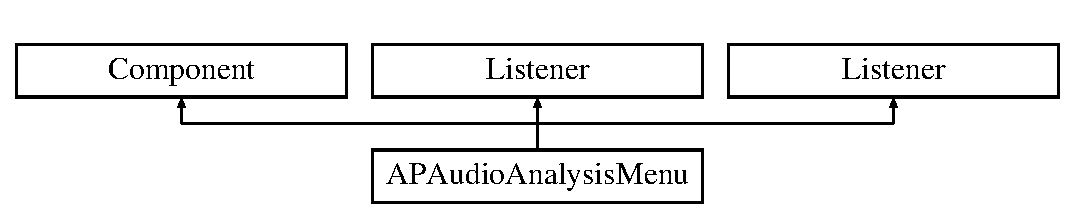
\includegraphics[height=2.000000cm]{class_a_p_audio_analysis_menu}
\end{center}
\end{figure}
\subsection*{Public Member Functions}
\begin{DoxyCompactItemize}
\item 
\hyperlink{class_a_p_audio_analysis_menu_a9480d205d954e579e923948456e69c46}{A\+P\+Audio\+Analysis\+Menu} (\hyperlink{class_a_p_audio_file_manager}{A\+P\+Audio\+File\+Manager} $\ast$file\+Manager, \hyperlink{class_a_p_audio_window_manager}{A\+P\+Audio\+Window\+Manager} $\ast$window\+Manager, \hyperlink{class_wave_form_component}{Wave\+Form\+Component} $\ast$waveform\+Component)
\item 
\hyperlink{class_a_p_audio_analysis_menu_aa1e4aec667d83a92538ba667b18186f2}{$\sim$\+A\+P\+Audio\+Analysis\+Menu} ()
\item 
void \hyperlink{class_a_p_audio_analysis_menu_a6d6edd5163984612f26da6edfd809306}{resized} () overridefinal
\item 
void \hyperlink{class_a_p_audio_analysis_menu_a6b5beba42dafb8645b1b30416c30fd04}{paint} (Graphics \&g) overridefinal
\item 
void \hyperlink{class_a_p_audio_analysis_menu_a4811c18104da88a1986d1e50a1796bb0}{button\+Clicked} (Button $\ast$button\+That\+Whas\+Clicked) overridefinal
\item 
void \hyperlink{class_a_p_audio_analysis_menu_a9f88e5c64f4e35cdb295c901b42682cb}{combo\+Box\+Changed} (Combo\+Box $\ast$combo\+Box\+That\+Has\+Changed) overridefinal
\end{DoxyCompactItemize}


\subsection{Constructor \& Destructor Documentation}
\hypertarget{class_a_p_audio_analysis_menu_a9480d205d954e579e923948456e69c46}{\index{A\+P\+Audio\+Analysis\+Menu@{A\+P\+Audio\+Analysis\+Menu}!A\+P\+Audio\+Analysis\+Menu@{A\+P\+Audio\+Analysis\+Menu}}
\index{A\+P\+Audio\+Analysis\+Menu@{A\+P\+Audio\+Analysis\+Menu}!A\+P\+Audio\+Analysis\+Menu@{A\+P\+Audio\+Analysis\+Menu}}
\subsubsection[{A\+P\+Audio\+Analysis\+Menu}]{\setlength{\rightskip}{0pt plus 5cm}A\+P\+Audio\+Analysis\+Menu\+::\+A\+P\+Audio\+Analysis\+Menu (
\begin{DoxyParamCaption}
\item[{{\bf A\+P\+Audio\+File\+Manager} $\ast$}]{file\+Manager, }
\item[{{\bf A\+P\+Audio\+Window\+Manager} $\ast$}]{window\+Manager, }
\item[{{\bf Wave\+Form\+Component} $\ast$}]{waveform\+Component}
\end{DoxyParamCaption}
)}}\label{class_a_p_audio_analysis_menu_a9480d205d954e579e923948456e69c46}
\hypertarget{class_a_p_audio_analysis_menu_aa1e4aec667d83a92538ba667b18186f2}{\index{A\+P\+Audio\+Analysis\+Menu@{A\+P\+Audio\+Analysis\+Menu}!````~A\+P\+Audio\+Analysis\+Menu@{$\sim$\+A\+P\+Audio\+Analysis\+Menu}}
\index{````~A\+P\+Audio\+Analysis\+Menu@{$\sim$\+A\+P\+Audio\+Analysis\+Menu}!A\+P\+Audio\+Analysis\+Menu@{A\+P\+Audio\+Analysis\+Menu}}
\subsubsection[{$\sim$\+A\+P\+Audio\+Analysis\+Menu}]{\setlength{\rightskip}{0pt plus 5cm}A\+P\+Audio\+Analysis\+Menu\+::$\sim$\+A\+P\+Audio\+Analysis\+Menu (
\begin{DoxyParamCaption}
{}
\end{DoxyParamCaption}
)}}\label{class_a_p_audio_analysis_menu_aa1e4aec667d83a92538ba667b18186f2}


\subsection{Member Function Documentation}
\hypertarget{class_a_p_audio_analysis_menu_a4811c18104da88a1986d1e50a1796bb0}{\index{A\+P\+Audio\+Analysis\+Menu@{A\+P\+Audio\+Analysis\+Menu}!button\+Clicked@{button\+Clicked}}
\index{button\+Clicked@{button\+Clicked}!A\+P\+Audio\+Analysis\+Menu@{A\+P\+Audio\+Analysis\+Menu}}
\subsubsection[{button\+Clicked}]{\setlength{\rightskip}{0pt plus 5cm}void A\+P\+Audio\+Analysis\+Menu\+::button\+Clicked (
\begin{DoxyParamCaption}
\item[{Button $\ast$}]{button\+That\+Whas\+Clicked}
\end{DoxyParamCaption}
)\hspace{0.3cm}{\ttfamily [final]}, {\ttfamily [override]}}}\label{class_a_p_audio_analysis_menu_a4811c18104da88a1986d1e50a1796bb0}
\hypertarget{class_a_p_audio_analysis_menu_a9f88e5c64f4e35cdb295c901b42682cb}{\index{A\+P\+Audio\+Analysis\+Menu@{A\+P\+Audio\+Analysis\+Menu}!combo\+Box\+Changed@{combo\+Box\+Changed}}
\index{combo\+Box\+Changed@{combo\+Box\+Changed}!A\+P\+Audio\+Analysis\+Menu@{A\+P\+Audio\+Analysis\+Menu}}
\subsubsection[{combo\+Box\+Changed}]{\setlength{\rightskip}{0pt plus 5cm}void A\+P\+Audio\+Analysis\+Menu\+::combo\+Box\+Changed (
\begin{DoxyParamCaption}
\item[{Combo\+Box $\ast$}]{combo\+Box\+That\+Has\+Changed}
\end{DoxyParamCaption}
)\hspace{0.3cm}{\ttfamily [final]}, {\ttfamily [override]}}}\label{class_a_p_audio_analysis_menu_a9f88e5c64f4e35cdb295c901b42682cb}
\hypertarget{class_a_p_audio_analysis_menu_a6b5beba42dafb8645b1b30416c30fd04}{\index{A\+P\+Audio\+Analysis\+Menu@{A\+P\+Audio\+Analysis\+Menu}!paint@{paint}}
\index{paint@{paint}!A\+P\+Audio\+Analysis\+Menu@{A\+P\+Audio\+Analysis\+Menu}}
\subsubsection[{paint}]{\setlength{\rightskip}{0pt plus 5cm}void A\+P\+Audio\+Analysis\+Menu\+::paint (
\begin{DoxyParamCaption}
\item[{Graphics \&}]{g}
\end{DoxyParamCaption}
)\hspace{0.3cm}{\ttfamily [final]}, {\ttfamily [override]}}}\label{class_a_p_audio_analysis_menu_a6b5beba42dafb8645b1b30416c30fd04}
\hypertarget{class_a_p_audio_analysis_menu_a6d6edd5163984612f26da6edfd809306}{\index{A\+P\+Audio\+Analysis\+Menu@{A\+P\+Audio\+Analysis\+Menu}!resized@{resized}}
\index{resized@{resized}!A\+P\+Audio\+Analysis\+Menu@{A\+P\+Audio\+Analysis\+Menu}}
\subsubsection[{resized}]{\setlength{\rightskip}{0pt plus 5cm}void A\+P\+Audio\+Analysis\+Menu\+::resized (
\begin{DoxyParamCaption}
{}
\end{DoxyParamCaption}
)\hspace{0.3cm}{\ttfamily [final]}, {\ttfamily [override]}}}\label{class_a_p_audio_analysis_menu_a6d6edd5163984612f26da6edfd809306}


The documentation for this class was generated from the following files\+:\begin{DoxyCompactItemize}
\item 
G\+U\+I Classes/\+Headers/\hyperlink{_a_p_audio_analysis_menu_8h}{A\+P\+Audio\+Analysis\+Menu.\+h}\item 
G\+U\+I Classes/\+Implementations/\hyperlink{_a_p_audio_analysis_menu_8cpp}{A\+P\+Audio\+Analysis\+Menu.\+cpp}\end{DoxyCompactItemize}

\hypertarget{class_a_p_audio_decimator_module}{\section{A\+P\+Audio\+Decimator\+Module Class Reference}
\label{class_a_p_audio_decimator_module}\index{A\+P\+Audio\+Decimator\+Module@{A\+P\+Audio\+Decimator\+Module}}
}


{\ttfamily \#include $<$A\+P\+Audio\+Decimator\+Module.\+h$>$}

Inheritance diagram for A\+P\+Audio\+Decimator\+Module\+:\begin{figure}[H]
\begin{center}
\leavevmode
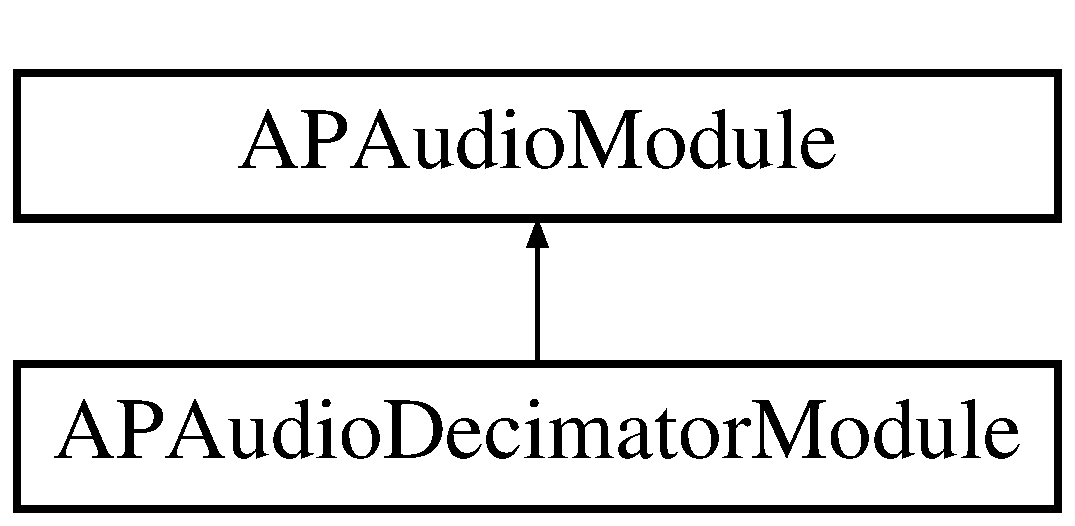
\includegraphics[height=2.000000cm]{class_a_p_audio_decimator_module}
\end{center}
\end{figure}
\subsection*{Public Member Functions}
\begin{DoxyCompactItemize}
\item 
\hyperlink{class_a_p_audio_decimator_module_a6fa88d486504734d4007bc89638f4254}{A\+P\+Audio\+Decimator\+Module} (\hyperlink{class_a_p_audio_main_frame}{A\+P\+Audio\+Main\+Frame} $\ast$mf)
\item 
void \hyperlink{class_a_p_audio_decimator_module_aeb5165253ed1286fd5a545150a016aae}{calculate\+Buffer} () overridefinal
\item 
void \hyperlink{class_a_p_audio_decimator_module_a1c9ff1ab4eceefa8dcee03db0e2fa109}{set\+Bit\+Rate} (\hyperlink{_a_p_audio_module_8h_a9cc0620fb2e91b51587c6936060d4161}{U\+Int} rate)
\item 
\hyperlink{_a_p_audio_module_8h_a9cc0620fb2e91b51587c6936060d4161}{U\+Int} \hyperlink{class_a_p_audio_decimator_module_a34201704335c3ba92524e024a9c6e7ee}{get\+Bit\+Rate} ()
\end{DoxyCompactItemize}
\subsection*{Additional Inherited Members}


\subsection{Constructor \& Destructor Documentation}
\hypertarget{class_a_p_audio_decimator_module_a6fa88d486504734d4007bc89638f4254}{\index{A\+P\+Audio\+Decimator\+Module@{A\+P\+Audio\+Decimator\+Module}!A\+P\+Audio\+Decimator\+Module@{A\+P\+Audio\+Decimator\+Module}}
\index{A\+P\+Audio\+Decimator\+Module@{A\+P\+Audio\+Decimator\+Module}!A\+P\+Audio\+Decimator\+Module@{A\+P\+Audio\+Decimator\+Module}}
\subsubsection[{A\+P\+Audio\+Decimator\+Module}]{\setlength{\rightskip}{0pt plus 5cm}A\+P\+Audio\+Decimator\+Module\+::\+A\+P\+Audio\+Decimator\+Module (
\begin{DoxyParamCaption}
\item[{{\bf A\+P\+Audio\+Main\+Frame} $\ast$}]{mf}
\end{DoxyParamCaption}
)}}\label{class_a_p_audio_decimator_module_a6fa88d486504734d4007bc89638f4254}


\subsection{Member Function Documentation}
\hypertarget{class_a_p_audio_decimator_module_aeb5165253ed1286fd5a545150a016aae}{\index{A\+P\+Audio\+Decimator\+Module@{A\+P\+Audio\+Decimator\+Module}!calculate\+Buffer@{calculate\+Buffer}}
\index{calculate\+Buffer@{calculate\+Buffer}!A\+P\+Audio\+Decimator\+Module@{A\+P\+Audio\+Decimator\+Module}}
\subsubsection[{calculate\+Buffer}]{\setlength{\rightskip}{0pt plus 5cm}void A\+P\+Audio\+Decimator\+Module\+::calculate\+Buffer (
\begin{DoxyParamCaption}
{}
\end{DoxyParamCaption}
)\hspace{0.3cm}{\ttfamily [final]}, {\ttfamily [override]}, {\ttfamily [virtual]}}}\label{class_a_p_audio_decimator_module_aeb5165253ed1286fd5a545150a016aae}


Reimplemented from \hyperlink{class_a_p_audio_module_a10c6d7f469b9d1626a80c4d745663a2a}{A\+P\+Audio\+Module}.

\hypertarget{class_a_p_audio_decimator_module_a34201704335c3ba92524e024a9c6e7ee}{\index{A\+P\+Audio\+Decimator\+Module@{A\+P\+Audio\+Decimator\+Module}!get\+Bit\+Rate@{get\+Bit\+Rate}}
\index{get\+Bit\+Rate@{get\+Bit\+Rate}!A\+P\+Audio\+Decimator\+Module@{A\+P\+Audio\+Decimator\+Module}}
\subsubsection[{get\+Bit\+Rate}]{\setlength{\rightskip}{0pt plus 5cm}{\bf U\+Int} A\+P\+Audio\+Decimator\+Module\+::get\+Bit\+Rate (
\begin{DoxyParamCaption}
{}
\end{DoxyParamCaption}
)\hspace{0.3cm}{\ttfamily [inline]}}}\label{class_a_p_audio_decimator_module_a34201704335c3ba92524e024a9c6e7ee}
\hypertarget{class_a_p_audio_decimator_module_a1c9ff1ab4eceefa8dcee03db0e2fa109}{\index{A\+P\+Audio\+Decimator\+Module@{A\+P\+Audio\+Decimator\+Module}!set\+Bit\+Rate@{set\+Bit\+Rate}}
\index{set\+Bit\+Rate@{set\+Bit\+Rate}!A\+P\+Audio\+Decimator\+Module@{A\+P\+Audio\+Decimator\+Module}}
\subsubsection[{set\+Bit\+Rate}]{\setlength{\rightskip}{0pt plus 5cm}void A\+P\+Audio\+Decimator\+Module\+::set\+Bit\+Rate (
\begin{DoxyParamCaption}
\item[{{\bf U\+Int}}]{rate}
\end{DoxyParamCaption}
)}}\label{class_a_p_audio_decimator_module_a1c9ff1ab4eceefa8dcee03db0e2fa109}


The documentation for this class was generated from the following files\+:\begin{DoxyCompactItemize}
\item 
Audio Classes/\+Headers/\hyperlink{_a_p_audio_decimator_module_8h}{A\+P\+Audio\+Decimator\+Module.\+h}\item 
Audio Classes/\+Implementations/\hyperlink{_a_p_audio_decimator_module_8cpp}{A\+P\+Audio\+Decimator\+Module.\+cpp}\end{DoxyCompactItemize}

\hypertarget{class_a_p_audio_envelope}{\section{A\+P\+Audio\+Envelope Class Reference}
\label{class_a_p_audio_envelope}\index{A\+P\+Audio\+Envelope@{A\+P\+Audio\+Envelope}}
}


{\ttfamily \#include $<$A\+P\+Audio\+Envelope.\+h$>$}

\subsection*{Public Types}
\begin{DoxyCompactItemize}
\item 
enum \hyperlink{class_a_p_audio_envelope_aed3a129a289360005327919f10ce02b9}{Envelope\+State} \{ \\*
\hyperlink{class_a_p_audio_envelope_aed3a129a289360005327919f10ce02b9a1d3e450a9f1f26eeffb3515b8b8bbeaf}{O\+F\+F}, 
\hyperlink{class_a_p_audio_envelope_aed3a129a289360005327919f10ce02b9a86b388b5455684cec6b24f2c27032071}{A\+T\+T\+A\+C\+K}, 
\hyperlink{class_a_p_audio_envelope_aed3a129a289360005327919f10ce02b9ac27b787b02a255670fe4a44efe61e912}{D\+E\+C\+A\+Y}, 
\hyperlink{class_a_p_audio_envelope_aed3a129a289360005327919f10ce02b9a64a32d0bacf8822b287b24f77ec2b68d}{S\+U\+S\+T\+A\+I\+N}, 
\\*
\hyperlink{class_a_p_audio_envelope_aed3a129a289360005327919f10ce02b9aa669da511b590c1315163fe4166f675b}{R\+E\+L\+E\+A\+S\+E}, 
\hyperlink{class_a_p_audio_envelope_aed3a129a289360005327919f10ce02b9a0607abcd44cb1aaad09f8a5f6503e403}{N\+U\+M\+S\+T\+A\+T\+E\+S}
 \}
\end{DoxyCompactItemize}
\subsection*{Public Member Functions}
\begin{DoxyCompactItemize}
\item 
\hyperlink{class_a_p_audio_envelope_a6e29c4b6f4d1e9e3344073fc5934487a}{A\+P\+Audio\+Envelope} ()
\item 
\hyperlink{_a_p_audio_module_8h_a9219378a2632ccf0389d00317ce8cdc4}{Control\+Value} \hyperlink{class_a_p_audio_envelope_a9d2da7832ecf1e6434420b6fbed1f9ce}{get\+Amplitude} ()
\item 
void \hyperlink{class_a_p_audio_envelope_af1267f79ac5b3e5524a1637f9746356d}{calculate\+Multiplier} (\hyperlink{_a_p_audio_module_8h_a9219378a2632ccf0389d00317ce8cdc4}{Control\+Value} start\+Level, \hyperlink{_a_p_audio_module_8h_a9219378a2632ccf0389d00317ce8cdc4}{Control\+Value} end\+Level, \hyperlink{_a_p_audio_module_8h_a7d836cc51adbed3f66d5c4c91ed72e94}{Timer\+Value} time)
\item 
void \hyperlink{class_a_p_audio_envelope_ae981e46fc12b69f92a19852b9fb99d1c}{enter\+Next\+Stage} (\hyperlink{class_a_p_audio_envelope_aed3a129a289360005327919f10ce02b9}{Envelope\+State} state)
\item 
\hyperlink{class_a_p_audio_envelope_aed3a129a289360005327919f10ce02b9}{Envelope\+State} \hyperlink{class_a_p_audio_envelope_af4e278663ff265641e0b155de35dedc8}{get\+Current\+State} () const 
\end{DoxyCompactItemize}


\subsection{Member Enumeration Documentation}
\hypertarget{class_a_p_audio_envelope_aed3a129a289360005327919f10ce02b9}{\index{A\+P\+Audio\+Envelope@{A\+P\+Audio\+Envelope}!Envelope\+State@{Envelope\+State}}
\index{Envelope\+State@{Envelope\+State}!A\+P\+Audio\+Envelope@{A\+P\+Audio\+Envelope}}
\subsubsection[{Envelope\+State}]{\setlength{\rightskip}{0pt plus 5cm}enum {\bf A\+P\+Audio\+Envelope\+::\+Envelope\+State}}}\label{class_a_p_audio_envelope_aed3a129a289360005327919f10ce02b9}
\begin{Desc}
\item[Enumerator]\par
\begin{description}
\index{O\+F\+F@{O\+F\+F}!A\+P\+Audio\+Envelope@{A\+P\+Audio\+Envelope}}\index{A\+P\+Audio\+Envelope@{A\+P\+Audio\+Envelope}!O\+F\+F@{O\+F\+F}}\item[{\em 
\hypertarget{class_a_p_audio_envelope_aed3a129a289360005327919f10ce02b9a1d3e450a9f1f26eeffb3515b8b8bbeaf}{O\+F\+F}\label{class_a_p_audio_envelope_aed3a129a289360005327919f10ce02b9a1d3e450a9f1f26eeffb3515b8b8bbeaf}
}]\index{A\+T\+T\+A\+C\+K@{A\+T\+T\+A\+C\+K}!A\+P\+Audio\+Envelope@{A\+P\+Audio\+Envelope}}\index{A\+P\+Audio\+Envelope@{A\+P\+Audio\+Envelope}!A\+T\+T\+A\+C\+K@{A\+T\+T\+A\+C\+K}}\item[{\em 
\hypertarget{class_a_p_audio_envelope_aed3a129a289360005327919f10ce02b9a86b388b5455684cec6b24f2c27032071}{A\+T\+T\+A\+C\+K}\label{class_a_p_audio_envelope_aed3a129a289360005327919f10ce02b9a86b388b5455684cec6b24f2c27032071}
}]\index{D\+E\+C\+A\+Y@{D\+E\+C\+A\+Y}!A\+P\+Audio\+Envelope@{A\+P\+Audio\+Envelope}}\index{A\+P\+Audio\+Envelope@{A\+P\+Audio\+Envelope}!D\+E\+C\+A\+Y@{D\+E\+C\+A\+Y}}\item[{\em 
\hypertarget{class_a_p_audio_envelope_aed3a129a289360005327919f10ce02b9ac27b787b02a255670fe4a44efe61e912}{D\+E\+C\+A\+Y}\label{class_a_p_audio_envelope_aed3a129a289360005327919f10ce02b9ac27b787b02a255670fe4a44efe61e912}
}]\index{S\+U\+S\+T\+A\+I\+N@{S\+U\+S\+T\+A\+I\+N}!A\+P\+Audio\+Envelope@{A\+P\+Audio\+Envelope}}\index{A\+P\+Audio\+Envelope@{A\+P\+Audio\+Envelope}!S\+U\+S\+T\+A\+I\+N@{S\+U\+S\+T\+A\+I\+N}}\item[{\em 
\hypertarget{class_a_p_audio_envelope_aed3a129a289360005327919f10ce02b9a64a32d0bacf8822b287b24f77ec2b68d}{S\+U\+S\+T\+A\+I\+N}\label{class_a_p_audio_envelope_aed3a129a289360005327919f10ce02b9a64a32d0bacf8822b287b24f77ec2b68d}
}]\index{R\+E\+L\+E\+A\+S\+E@{R\+E\+L\+E\+A\+S\+E}!A\+P\+Audio\+Envelope@{A\+P\+Audio\+Envelope}}\index{A\+P\+Audio\+Envelope@{A\+P\+Audio\+Envelope}!R\+E\+L\+E\+A\+S\+E@{R\+E\+L\+E\+A\+S\+E}}\item[{\em 
\hypertarget{class_a_p_audio_envelope_aed3a129a289360005327919f10ce02b9aa669da511b590c1315163fe4166f675b}{R\+E\+L\+E\+A\+S\+E}\label{class_a_p_audio_envelope_aed3a129a289360005327919f10ce02b9aa669da511b590c1315163fe4166f675b}
}]\index{N\+U\+M\+S\+T\+A\+T\+E\+S@{N\+U\+M\+S\+T\+A\+T\+E\+S}!A\+P\+Audio\+Envelope@{A\+P\+Audio\+Envelope}}\index{A\+P\+Audio\+Envelope@{A\+P\+Audio\+Envelope}!N\+U\+M\+S\+T\+A\+T\+E\+S@{N\+U\+M\+S\+T\+A\+T\+E\+S}}\item[{\em 
\hypertarget{class_a_p_audio_envelope_aed3a129a289360005327919f10ce02b9a0607abcd44cb1aaad09f8a5f6503e403}{N\+U\+M\+S\+T\+A\+T\+E\+S}\label{class_a_p_audio_envelope_aed3a129a289360005327919f10ce02b9a0607abcd44cb1aaad09f8a5f6503e403}
}]\end{description}
\end{Desc}


\subsection{Constructor \& Destructor Documentation}
\hypertarget{class_a_p_audio_envelope_a6e29c4b6f4d1e9e3344073fc5934487a}{\index{A\+P\+Audio\+Envelope@{A\+P\+Audio\+Envelope}!A\+P\+Audio\+Envelope@{A\+P\+Audio\+Envelope}}
\index{A\+P\+Audio\+Envelope@{A\+P\+Audio\+Envelope}!A\+P\+Audio\+Envelope@{A\+P\+Audio\+Envelope}}
\subsubsection[{A\+P\+Audio\+Envelope}]{\setlength{\rightskip}{0pt plus 5cm}A\+P\+Audio\+Envelope\+::\+A\+P\+Audio\+Envelope (
\begin{DoxyParamCaption}
{}
\end{DoxyParamCaption}
)}}\label{class_a_p_audio_envelope_a6e29c4b6f4d1e9e3344073fc5934487a}


\subsection{Member Function Documentation}
\hypertarget{class_a_p_audio_envelope_af1267f79ac5b3e5524a1637f9746356d}{\index{A\+P\+Audio\+Envelope@{A\+P\+Audio\+Envelope}!calculate\+Multiplier@{calculate\+Multiplier}}
\index{calculate\+Multiplier@{calculate\+Multiplier}!A\+P\+Audio\+Envelope@{A\+P\+Audio\+Envelope}}
\subsubsection[{calculate\+Multiplier}]{\setlength{\rightskip}{0pt plus 5cm}void A\+P\+Audio\+Envelope\+::calculate\+Multiplier (
\begin{DoxyParamCaption}
\item[{{\bf Control\+Value}}]{start\+Level, }
\item[{{\bf Control\+Value}}]{end\+Level, }
\item[{{\bf Timer\+Value}}]{time}
\end{DoxyParamCaption}
)}}\label{class_a_p_audio_envelope_af1267f79ac5b3e5524a1637f9746356d}
\hypertarget{class_a_p_audio_envelope_ae981e46fc12b69f92a19852b9fb99d1c}{\index{A\+P\+Audio\+Envelope@{A\+P\+Audio\+Envelope}!enter\+Next\+Stage@{enter\+Next\+Stage}}
\index{enter\+Next\+Stage@{enter\+Next\+Stage}!A\+P\+Audio\+Envelope@{A\+P\+Audio\+Envelope}}
\subsubsection[{enter\+Next\+Stage}]{\setlength{\rightskip}{0pt plus 5cm}void A\+P\+Audio\+Envelope\+::enter\+Next\+Stage (
\begin{DoxyParamCaption}
\item[{{\bf A\+P\+Audio\+Envelope\+::\+Envelope\+State}}]{state}
\end{DoxyParamCaption}
)}}\label{class_a_p_audio_envelope_ae981e46fc12b69f92a19852b9fb99d1c}
\hypertarget{class_a_p_audio_envelope_a9d2da7832ecf1e6434420b6fbed1f9ce}{\index{A\+P\+Audio\+Envelope@{A\+P\+Audio\+Envelope}!get\+Amplitude@{get\+Amplitude}}
\index{get\+Amplitude@{get\+Amplitude}!A\+P\+Audio\+Envelope@{A\+P\+Audio\+Envelope}}
\subsubsection[{get\+Amplitude}]{\setlength{\rightskip}{0pt plus 5cm}{\bf Control\+Value} A\+P\+Audio\+Envelope\+::get\+Amplitude (
\begin{DoxyParamCaption}
{}
\end{DoxyParamCaption}
)}}\label{class_a_p_audio_envelope_a9d2da7832ecf1e6434420b6fbed1f9ce}
\hypertarget{class_a_p_audio_envelope_af4e278663ff265641e0b155de35dedc8}{\index{A\+P\+Audio\+Envelope@{A\+P\+Audio\+Envelope}!get\+Current\+State@{get\+Current\+State}}
\index{get\+Current\+State@{get\+Current\+State}!A\+P\+Audio\+Envelope@{A\+P\+Audio\+Envelope}}
\subsubsection[{get\+Current\+State}]{\setlength{\rightskip}{0pt plus 5cm}{\bf Envelope\+State} A\+P\+Audio\+Envelope\+::get\+Current\+State (
\begin{DoxyParamCaption}
{}
\end{DoxyParamCaption}
) const\hspace{0.3cm}{\ttfamily [inline]}}}\label{class_a_p_audio_envelope_af4e278663ff265641e0b155de35dedc8}


The documentation for this class was generated from the following files\+:\begin{DoxyCompactItemize}
\item 
Audio Classes/\+Headers/\hyperlink{_a_p_audio_envelope_8h}{A\+P\+Audio\+Envelope.\+h}\item 
Audio Classes/\+Implementations/\hyperlink{_a_p_audio_envelope_8cpp}{A\+P\+Audio\+Envelope.\+cpp}\end{DoxyCompactItemize}

\hypertarget{class_a_p_audio_file}{\section{A\+P\+Audio\+File Class Reference}
\label{class_a_p_audio_file}\index{A\+P\+Audio\+File@{A\+P\+Audio\+File}}
}


{\ttfamily \#include $<$A\+P\+Audio\+File.\+h$>$}

\subsection*{Public Member Functions}
\begin{DoxyCompactItemize}
\item 
\hyperlink{class_a_p_audio_file_a1139a3105847950da22822fd9518a3b9}{$\sim$\+A\+P\+Audio\+File} ()
\item 
void \hyperlink{class_a_p_audio_file_a07d1b051ca1b498187bbf5a5d9439af3}{set\+Audio} (Audio\+Sample\+Buffer buffer)
\item 
void \hyperlink{class_a_p_audio_file_a453184afd4e48694e0bed36459fb7641}{set\+Num\+Channels} (int channels)
\item 
void \hyperlink{class_a_p_audio_file_abce32907787e6fb546861e9085aba9e2}{set\+Num\+Samples} (long int samples)
\item 
void \hyperlink{class_a_p_audio_file_a02940af3dd917491796347acd197aa30}{set\+File\+Name} (String name)
\item 
void \hyperlink{class_a_p_audio_file_a396c24cbfbe2b65db24d1f62e324202b}{set\+Samplerate} (int sample\+Rate)
\item 
String \hyperlink{class_a_p_audio_file_acb1dceb8d5ab6d5cf37f9fc880bcfbba}{get\+Name} ()
\item 
const float $\ast$ \hyperlink{class_a_p_audio_file_a648534146533efbab0f23138f9b9bd3c}{get\+Audio\+Channel} (int index)
\item 
int \hyperlink{class_a_p_audio_file_a6e81aaf02553821367017388f08ea603}{get\+Num\+Channels} ()
\item 
long int \hyperlink{class_a_p_audio_file_a7b29d23f6b306c75be3cda81c3f7b470}{get\+Num\+Samples} ()
\item 
int \hyperlink{class_a_p_audio_file_a14b346948198b6f99806e5e30c1a5839}{get\+Sample\+Rate} ()
\end{DoxyCompactItemize}


\subsection{Constructor \& Destructor Documentation}
\hypertarget{class_a_p_audio_file_a1139a3105847950da22822fd9518a3b9}{\index{A\+P\+Audio\+File@{A\+P\+Audio\+File}!````~A\+P\+Audio\+File@{$\sim$\+A\+P\+Audio\+File}}
\index{````~A\+P\+Audio\+File@{$\sim$\+A\+P\+Audio\+File}!A\+P\+Audio\+File@{A\+P\+Audio\+File}}
\subsubsection[{$\sim$\+A\+P\+Audio\+File}]{\setlength{\rightskip}{0pt plus 5cm}A\+P\+Audio\+File\+::$\sim$\+A\+P\+Audio\+File (
\begin{DoxyParamCaption}
{}
\end{DoxyParamCaption}
)}}\label{class_a_p_audio_file_a1139a3105847950da22822fd9518a3b9}


\subsection{Member Function Documentation}
\hypertarget{class_a_p_audio_file_a648534146533efbab0f23138f9b9bd3c}{\index{A\+P\+Audio\+File@{A\+P\+Audio\+File}!get\+Audio\+Channel@{get\+Audio\+Channel}}
\index{get\+Audio\+Channel@{get\+Audio\+Channel}!A\+P\+Audio\+File@{A\+P\+Audio\+File}}
\subsubsection[{get\+Audio\+Channel}]{\setlength{\rightskip}{0pt plus 5cm}const float $\ast$ A\+P\+Audio\+File\+::get\+Audio\+Channel (
\begin{DoxyParamCaption}
\item[{int}]{index}
\end{DoxyParamCaption}
)}}\label{class_a_p_audio_file_a648534146533efbab0f23138f9b9bd3c}
\hypertarget{class_a_p_audio_file_acb1dceb8d5ab6d5cf37f9fc880bcfbba}{\index{A\+P\+Audio\+File@{A\+P\+Audio\+File}!get\+Name@{get\+Name}}
\index{get\+Name@{get\+Name}!A\+P\+Audio\+File@{A\+P\+Audio\+File}}
\subsubsection[{get\+Name}]{\setlength{\rightskip}{0pt plus 5cm}String A\+P\+Audio\+File\+::get\+Name (
\begin{DoxyParamCaption}
{}
\end{DoxyParamCaption}
)}}\label{class_a_p_audio_file_acb1dceb8d5ab6d5cf37f9fc880bcfbba}
\hypertarget{class_a_p_audio_file_a6e81aaf02553821367017388f08ea603}{\index{A\+P\+Audio\+File@{A\+P\+Audio\+File}!get\+Num\+Channels@{get\+Num\+Channels}}
\index{get\+Num\+Channels@{get\+Num\+Channels}!A\+P\+Audio\+File@{A\+P\+Audio\+File}}
\subsubsection[{get\+Num\+Channels}]{\setlength{\rightskip}{0pt plus 5cm}int A\+P\+Audio\+File\+::get\+Num\+Channels (
\begin{DoxyParamCaption}
{}
\end{DoxyParamCaption}
)}}\label{class_a_p_audio_file_a6e81aaf02553821367017388f08ea603}
\hypertarget{class_a_p_audio_file_a7b29d23f6b306c75be3cda81c3f7b470}{\index{A\+P\+Audio\+File@{A\+P\+Audio\+File}!get\+Num\+Samples@{get\+Num\+Samples}}
\index{get\+Num\+Samples@{get\+Num\+Samples}!A\+P\+Audio\+File@{A\+P\+Audio\+File}}
\subsubsection[{get\+Num\+Samples}]{\setlength{\rightskip}{0pt plus 5cm}long int A\+P\+Audio\+File\+::get\+Num\+Samples (
\begin{DoxyParamCaption}
{}
\end{DoxyParamCaption}
)}}\label{class_a_p_audio_file_a7b29d23f6b306c75be3cda81c3f7b470}
\hypertarget{class_a_p_audio_file_a14b346948198b6f99806e5e30c1a5839}{\index{A\+P\+Audio\+File@{A\+P\+Audio\+File}!get\+Sample\+Rate@{get\+Sample\+Rate}}
\index{get\+Sample\+Rate@{get\+Sample\+Rate}!A\+P\+Audio\+File@{A\+P\+Audio\+File}}
\subsubsection[{get\+Sample\+Rate}]{\setlength{\rightskip}{0pt plus 5cm}int A\+P\+Audio\+File\+::get\+Sample\+Rate (
\begin{DoxyParamCaption}
{}
\end{DoxyParamCaption}
)}}\label{class_a_p_audio_file_a14b346948198b6f99806e5e30c1a5839}
\hypertarget{class_a_p_audio_file_a07d1b051ca1b498187bbf5a5d9439af3}{\index{A\+P\+Audio\+File@{A\+P\+Audio\+File}!set\+Audio@{set\+Audio}}
\index{set\+Audio@{set\+Audio}!A\+P\+Audio\+File@{A\+P\+Audio\+File}}
\subsubsection[{set\+Audio}]{\setlength{\rightskip}{0pt plus 5cm}void A\+P\+Audio\+File\+::set\+Audio (
\begin{DoxyParamCaption}
\item[{Audio\+Sample\+Buffer}]{buffer}
\end{DoxyParamCaption}
)}}\label{class_a_p_audio_file_a07d1b051ca1b498187bbf5a5d9439af3}
\hypertarget{class_a_p_audio_file_a02940af3dd917491796347acd197aa30}{\index{A\+P\+Audio\+File@{A\+P\+Audio\+File}!set\+File\+Name@{set\+File\+Name}}
\index{set\+File\+Name@{set\+File\+Name}!A\+P\+Audio\+File@{A\+P\+Audio\+File}}
\subsubsection[{set\+File\+Name}]{\setlength{\rightskip}{0pt plus 5cm}void A\+P\+Audio\+File\+::set\+File\+Name (
\begin{DoxyParamCaption}
\item[{String}]{name}
\end{DoxyParamCaption}
)}}\label{class_a_p_audio_file_a02940af3dd917491796347acd197aa30}
\hypertarget{class_a_p_audio_file_a453184afd4e48694e0bed36459fb7641}{\index{A\+P\+Audio\+File@{A\+P\+Audio\+File}!set\+Num\+Channels@{set\+Num\+Channels}}
\index{set\+Num\+Channels@{set\+Num\+Channels}!A\+P\+Audio\+File@{A\+P\+Audio\+File}}
\subsubsection[{set\+Num\+Channels}]{\setlength{\rightskip}{0pt plus 5cm}void A\+P\+Audio\+File\+::set\+Num\+Channels (
\begin{DoxyParamCaption}
\item[{int}]{channels}
\end{DoxyParamCaption}
)}}\label{class_a_p_audio_file_a453184afd4e48694e0bed36459fb7641}
\hypertarget{class_a_p_audio_file_abce32907787e6fb546861e9085aba9e2}{\index{A\+P\+Audio\+File@{A\+P\+Audio\+File}!set\+Num\+Samples@{set\+Num\+Samples}}
\index{set\+Num\+Samples@{set\+Num\+Samples}!A\+P\+Audio\+File@{A\+P\+Audio\+File}}
\subsubsection[{set\+Num\+Samples}]{\setlength{\rightskip}{0pt plus 5cm}void A\+P\+Audio\+File\+::set\+Num\+Samples (
\begin{DoxyParamCaption}
\item[{long int}]{samples}
\end{DoxyParamCaption}
)}}\label{class_a_p_audio_file_abce32907787e6fb546861e9085aba9e2}
\hypertarget{class_a_p_audio_file_a396c24cbfbe2b65db24d1f62e324202b}{\index{A\+P\+Audio\+File@{A\+P\+Audio\+File}!set\+Samplerate@{set\+Samplerate}}
\index{set\+Samplerate@{set\+Samplerate}!A\+P\+Audio\+File@{A\+P\+Audio\+File}}
\subsubsection[{set\+Samplerate}]{\setlength{\rightskip}{0pt plus 5cm}void A\+P\+Audio\+File\+::set\+Samplerate (
\begin{DoxyParamCaption}
\item[{int}]{sample\+Rate}
\end{DoxyParamCaption}
)}}\label{class_a_p_audio_file_a396c24cbfbe2b65db24d1f62e324202b}


The documentation for this class was generated from the following files\+:\begin{DoxyCompactItemize}
\item 
Audio Classes/\+Headers/\hyperlink{_a_p_audio_file_8h}{A\+P\+Audio\+File.\+h}\item 
Audio Classes/\+Implementations/\hyperlink{_a_p_audio_file_8cpp}{A\+P\+Audio\+File.\+cpp}\end{DoxyCompactItemize}

\hypertarget{class_a_p_audio_file_manager}{\section{A\+P\+Audio\+File\+Manager Class Reference}
\label{class_a_p_audio_file_manager}\index{A\+P\+Audio\+File\+Manager@{A\+P\+Audio\+File\+Manager}}
}


{\ttfamily \#include $<$A\+P\+Audio\+File\+Manager2.\+h$>$}

\subsection*{Public Member Functions}
\begin{DoxyCompactItemize}
\item 
\hyperlink{class_a_p_audio_file_manager_a3a0dd7cfb1e16412c66f898511d46b34}{A\+P\+Audio\+File\+Manager} ()
\item 
\hyperlink{class_a_p_audio_file_manager_a1a1bb07cf3c8710c695c77cb6cd9baef}{$\sim$\+A\+P\+Audio\+File\+Manager} ()
\item 
void \hyperlink{class_a_p_audio_file_manager_ac07981ccd2caa78533d0399473aac33d}{load\+File} (File file\+To\+Load)
\item 
void \hyperlink{class_a_p_audio_file_manager_ac08c787e5180479048b53e0a5788ae98}{load\+File} (std\+::string file\+To\+Load)
\item 
void \hyperlink{class_a_p_audio_file_manager_a9968679e6778a46b45db09496eaf34ec}{load\+Files} ()
\item 
\hyperlink{class_a_p_audio_file}{A\+P\+Audio\+File} $\ast$ \hyperlink{class_a_p_audio_file_manager_a93197d9a8c4fd221a508713b000d5a98}{get\+File} (String name)
\item 
\hyperlink{class_a_p_audio_file}{A\+P\+Audio\+File} $\ast$ \hyperlink{class_a_p_audio_file_manager_a5d1cfd0ef9052f5185c3d75ae389c869}{get\+File} (int index)
\item 
void \hyperlink{class_a_p_audio_file_manager_a31affbe18da5e74ae2f06c660b62b0dc}{clear\+Manager} ()
\item 
int \hyperlink{class_a_p_audio_file_manager_a29bb102b0dea509bfedb280b0b8b2dac}{get\+Number\+Of\+Files} ()
\item 
\hyperlink{class_a_p_audio_file_manager_a3a0dd7cfb1e16412c66f898511d46b34}{A\+P\+Audio\+File\+Manager} ()
\item 
O\+S\+Status \hyperlink{class_a_p_audio_file_manager_a6d214b9b918cfae6c5ffdbc2ae8d4100}{get\+Available\+Sound\+File\+Libraries} ()
\item 
O\+S\+Status \hyperlink{class_a_p_audio_file_manager_a26d042ceefccb1c736975fac512a5c72}{get\+File\+List\+For\+Sound\+File\+Library} (N\+S\+String $\ast$library\+Name)
\item 
O\+S\+Status \hyperlink{class_a_p_audio_file_manager_ac23bd578b59c7baeab62802a1a7f4e50}{load\+File} (N\+S\+String $\ast$file\+Name, N\+S\+String $\ast$library\+Name)
\item 
O\+S\+Status \hyperlink{class_a_p_audio_file_manager_a7981965b1aa9f06eeef67c349211fb53}{setup\+Mono\+Stream\+Format} ()
\item 
O\+S\+Status \hyperlink{class_a_p_audio_file_manager_a761a4bdfa40e0a6bebfddede172c0a72}{setup\+Stereo\+Stream\+Format} ()
\item 
\hyperlink{struct_audio_file}{Audio\+File} $\ast$ \hyperlink{class_a_p_audio_file_manager_ac51cd969fe764d494a262522c1cca067}{find\+File} (std\+::string file\+Name)
\end{DoxyCompactItemize}


\subsection{Constructor \& Destructor Documentation}
\hypertarget{class_a_p_audio_file_manager_a3a0dd7cfb1e16412c66f898511d46b34}{\index{A\+P\+Audio\+File\+Manager@{A\+P\+Audio\+File\+Manager}!A\+P\+Audio\+File\+Manager@{A\+P\+Audio\+File\+Manager}}
\index{A\+P\+Audio\+File\+Manager@{A\+P\+Audio\+File\+Manager}!A\+P\+Audio\+File\+Manager@{A\+P\+Audio\+File\+Manager}}
\subsubsection[{A\+P\+Audio\+File\+Manager}]{\setlength{\rightskip}{0pt plus 5cm}A\+P\+Audio\+File\+Manager\+::\+A\+P\+Audio\+File\+Manager (
\begin{DoxyParamCaption}
{}
\end{DoxyParamCaption}
)}}\label{class_a_p_audio_file_manager_a3a0dd7cfb1e16412c66f898511d46b34}
\hypertarget{class_a_p_audio_file_manager_a1a1bb07cf3c8710c695c77cb6cd9baef}{\index{A\+P\+Audio\+File\+Manager@{A\+P\+Audio\+File\+Manager}!````~A\+P\+Audio\+File\+Manager@{$\sim$\+A\+P\+Audio\+File\+Manager}}
\index{````~A\+P\+Audio\+File\+Manager@{$\sim$\+A\+P\+Audio\+File\+Manager}!A\+P\+Audio\+File\+Manager@{A\+P\+Audio\+File\+Manager}}
\subsubsection[{$\sim$\+A\+P\+Audio\+File\+Manager}]{\setlength{\rightskip}{0pt plus 5cm}A\+P\+Audio\+File\+Manager\+::$\sim$\+A\+P\+Audio\+File\+Manager (
\begin{DoxyParamCaption}
{}
\end{DoxyParamCaption}
)}}\label{class_a_p_audio_file_manager_a1a1bb07cf3c8710c695c77cb6cd9baef}
\hypertarget{class_a_p_audio_file_manager_a3a0dd7cfb1e16412c66f898511d46b34}{\index{A\+P\+Audio\+File\+Manager@{A\+P\+Audio\+File\+Manager}!A\+P\+Audio\+File\+Manager@{A\+P\+Audio\+File\+Manager}}
\index{A\+P\+Audio\+File\+Manager@{A\+P\+Audio\+File\+Manager}!A\+P\+Audio\+File\+Manager@{A\+P\+Audio\+File\+Manager}}
\subsubsection[{A\+P\+Audio\+File\+Manager}]{\setlength{\rightskip}{0pt plus 5cm}A\+P\+Audio\+File\+Manager\+::\+A\+P\+Audio\+File\+Manager (
\begin{DoxyParamCaption}
{}
\end{DoxyParamCaption}
)}}\label{class_a_p_audio_file_manager_a3a0dd7cfb1e16412c66f898511d46b34}


\subsection{Member Function Documentation}
\hypertarget{class_a_p_audio_file_manager_a31affbe18da5e74ae2f06c660b62b0dc}{\index{A\+P\+Audio\+File\+Manager@{A\+P\+Audio\+File\+Manager}!clear\+Manager@{clear\+Manager}}
\index{clear\+Manager@{clear\+Manager}!A\+P\+Audio\+File\+Manager@{A\+P\+Audio\+File\+Manager}}
\subsubsection[{clear\+Manager}]{\setlength{\rightskip}{0pt plus 5cm}void A\+P\+Audio\+File\+Manager\+::clear\+Manager (
\begin{DoxyParamCaption}
{}
\end{DoxyParamCaption}
)}}\label{class_a_p_audio_file_manager_a31affbe18da5e74ae2f06c660b62b0dc}
\hypertarget{class_a_p_audio_file_manager_ac51cd969fe764d494a262522c1cca067}{\index{A\+P\+Audio\+File\+Manager@{A\+P\+Audio\+File\+Manager}!find\+File@{find\+File}}
\index{find\+File@{find\+File}!A\+P\+Audio\+File\+Manager@{A\+P\+Audio\+File\+Manager}}
\subsubsection[{find\+File}]{\setlength{\rightskip}{0pt plus 5cm}{\bf Audio\+File} $\ast$ A\+P\+Audio\+File\+Manager\+::find\+File (
\begin{DoxyParamCaption}
\item[{std\+::string}]{file\+Name}
\end{DoxyParamCaption}
)}}\label{class_a_p_audio_file_manager_ac51cd969fe764d494a262522c1cca067}
\hypertarget{class_a_p_audio_file_manager_a6d214b9b918cfae6c5ffdbc2ae8d4100}{\index{A\+P\+Audio\+File\+Manager@{A\+P\+Audio\+File\+Manager}!get\+Available\+Sound\+File\+Libraries@{get\+Available\+Sound\+File\+Libraries}}
\index{get\+Available\+Sound\+File\+Libraries@{get\+Available\+Sound\+File\+Libraries}!A\+P\+Audio\+File\+Manager@{A\+P\+Audio\+File\+Manager}}
\subsubsection[{get\+Available\+Sound\+File\+Libraries}]{\setlength{\rightskip}{0pt plus 5cm}O\+S\+Status A\+P\+Audio\+File\+Manager\+::get\+Available\+Sound\+File\+Libraries (
\begin{DoxyParamCaption}
{}
\end{DoxyParamCaption}
)}}\label{class_a_p_audio_file_manager_a6d214b9b918cfae6c5ffdbc2ae8d4100}
\hypertarget{class_a_p_audio_file_manager_a93197d9a8c4fd221a508713b000d5a98}{\index{A\+P\+Audio\+File\+Manager@{A\+P\+Audio\+File\+Manager}!get\+File@{get\+File}}
\index{get\+File@{get\+File}!A\+P\+Audio\+File\+Manager@{A\+P\+Audio\+File\+Manager}}
\subsubsection[{get\+File}]{\setlength{\rightskip}{0pt plus 5cm}{\bf A\+P\+Audio\+File}$\ast$ A\+P\+Audio\+File\+Manager\+::get\+File (
\begin{DoxyParamCaption}
\item[{String}]{name}
\end{DoxyParamCaption}
)}}\label{class_a_p_audio_file_manager_a93197d9a8c4fd221a508713b000d5a98}
\hypertarget{class_a_p_audio_file_manager_a5d1cfd0ef9052f5185c3d75ae389c869}{\index{A\+P\+Audio\+File\+Manager@{A\+P\+Audio\+File\+Manager}!get\+File@{get\+File}}
\index{get\+File@{get\+File}!A\+P\+Audio\+File\+Manager@{A\+P\+Audio\+File\+Manager}}
\subsubsection[{get\+File}]{\setlength{\rightskip}{0pt plus 5cm}{\bf A\+P\+Audio\+File} $\ast$ A\+P\+Audio\+File\+Manager\+::get\+File (
\begin{DoxyParamCaption}
\item[{int}]{index}
\end{DoxyParamCaption}
)}}\label{class_a_p_audio_file_manager_a5d1cfd0ef9052f5185c3d75ae389c869}
\hypertarget{class_a_p_audio_file_manager_a26d042ceefccb1c736975fac512a5c72}{\index{A\+P\+Audio\+File\+Manager@{A\+P\+Audio\+File\+Manager}!get\+File\+List\+For\+Sound\+File\+Library@{get\+File\+List\+For\+Sound\+File\+Library}}
\index{get\+File\+List\+For\+Sound\+File\+Library@{get\+File\+List\+For\+Sound\+File\+Library}!A\+P\+Audio\+File\+Manager@{A\+P\+Audio\+File\+Manager}}
\subsubsection[{get\+File\+List\+For\+Sound\+File\+Library}]{\setlength{\rightskip}{0pt plus 5cm}O\+S\+Status A\+P\+Audio\+File\+Manager\+::get\+File\+List\+For\+Sound\+File\+Library (
\begin{DoxyParamCaption}
\item[{N\+S\+String $\ast$}]{library\+Name}
\end{DoxyParamCaption}
)}}\label{class_a_p_audio_file_manager_a26d042ceefccb1c736975fac512a5c72}
\hypertarget{class_a_p_audio_file_manager_a29bb102b0dea509bfedb280b0b8b2dac}{\index{A\+P\+Audio\+File\+Manager@{A\+P\+Audio\+File\+Manager}!get\+Number\+Of\+Files@{get\+Number\+Of\+Files}}
\index{get\+Number\+Of\+Files@{get\+Number\+Of\+Files}!A\+P\+Audio\+File\+Manager@{A\+P\+Audio\+File\+Manager}}
\subsubsection[{get\+Number\+Of\+Files}]{\setlength{\rightskip}{0pt plus 5cm}int A\+P\+Audio\+File\+Manager\+::get\+Number\+Of\+Files (
\begin{DoxyParamCaption}
{}
\end{DoxyParamCaption}
)}}\label{class_a_p_audio_file_manager_a29bb102b0dea509bfedb280b0b8b2dac}
\hypertarget{class_a_p_audio_file_manager_ac07981ccd2caa78533d0399473aac33d}{\index{A\+P\+Audio\+File\+Manager@{A\+P\+Audio\+File\+Manager}!load\+File@{load\+File}}
\index{load\+File@{load\+File}!A\+P\+Audio\+File\+Manager@{A\+P\+Audio\+File\+Manager}}
\subsubsection[{load\+File}]{\setlength{\rightskip}{0pt plus 5cm}void A\+P\+Audio\+File\+Manager\+::load\+File (
\begin{DoxyParamCaption}
\item[{File}]{file\+To\+Load}
\end{DoxyParamCaption}
)}}\label{class_a_p_audio_file_manager_ac07981ccd2caa78533d0399473aac33d}
\hypertarget{class_a_p_audio_file_manager_ac08c787e5180479048b53e0a5788ae98}{\index{A\+P\+Audio\+File\+Manager@{A\+P\+Audio\+File\+Manager}!load\+File@{load\+File}}
\index{load\+File@{load\+File}!A\+P\+Audio\+File\+Manager@{A\+P\+Audio\+File\+Manager}}
\subsubsection[{load\+File}]{\setlength{\rightskip}{0pt plus 5cm}void A\+P\+Audio\+File\+Manager\+::load\+File (
\begin{DoxyParamCaption}
\item[{std\+::string}]{file\+To\+Load}
\end{DoxyParamCaption}
)}}\label{class_a_p_audio_file_manager_ac08c787e5180479048b53e0a5788ae98}
\hypertarget{class_a_p_audio_file_manager_ac23bd578b59c7baeab62802a1a7f4e50}{\index{A\+P\+Audio\+File\+Manager@{A\+P\+Audio\+File\+Manager}!load\+File@{load\+File}}
\index{load\+File@{load\+File}!A\+P\+Audio\+File\+Manager@{A\+P\+Audio\+File\+Manager}}
\subsubsection[{load\+File}]{\setlength{\rightskip}{0pt plus 5cm}O\+S\+Status A\+P\+Audio\+File\+Manager\+::load\+File (
\begin{DoxyParamCaption}
\item[{N\+S\+String $\ast$}]{file\+Name, }
\item[{N\+S\+String $\ast$}]{library\+Name}
\end{DoxyParamCaption}
)}}\label{class_a_p_audio_file_manager_ac23bd578b59c7baeab62802a1a7f4e50}
\hypertarget{class_a_p_audio_file_manager_a9968679e6778a46b45db09496eaf34ec}{\index{A\+P\+Audio\+File\+Manager@{A\+P\+Audio\+File\+Manager}!load\+Files@{load\+Files}}
\index{load\+Files@{load\+Files}!A\+P\+Audio\+File\+Manager@{A\+P\+Audio\+File\+Manager}}
\subsubsection[{load\+Files}]{\setlength{\rightskip}{0pt plus 5cm}void A\+P\+Audio\+File\+Manager\+::load\+Files (
\begin{DoxyParamCaption}
{}
\end{DoxyParamCaption}
)}}\label{class_a_p_audio_file_manager_a9968679e6778a46b45db09496eaf34ec}
\hypertarget{class_a_p_audio_file_manager_a7981965b1aa9f06eeef67c349211fb53}{\index{A\+P\+Audio\+File\+Manager@{A\+P\+Audio\+File\+Manager}!setup\+Mono\+Stream\+Format@{setup\+Mono\+Stream\+Format}}
\index{setup\+Mono\+Stream\+Format@{setup\+Mono\+Stream\+Format}!A\+P\+Audio\+File\+Manager@{A\+P\+Audio\+File\+Manager}}
\subsubsection[{setup\+Mono\+Stream\+Format}]{\setlength{\rightskip}{0pt plus 5cm}O\+S\+Status A\+P\+Audio\+File\+Manager\+::setup\+Mono\+Stream\+Format (
\begin{DoxyParamCaption}
{}
\end{DoxyParamCaption}
)}}\label{class_a_p_audio_file_manager_a7981965b1aa9f06eeef67c349211fb53}
\hypertarget{class_a_p_audio_file_manager_a761a4bdfa40e0a6bebfddede172c0a72}{\index{A\+P\+Audio\+File\+Manager@{A\+P\+Audio\+File\+Manager}!setup\+Stereo\+Stream\+Format@{setup\+Stereo\+Stream\+Format}}
\index{setup\+Stereo\+Stream\+Format@{setup\+Stereo\+Stream\+Format}!A\+P\+Audio\+File\+Manager@{A\+P\+Audio\+File\+Manager}}
\subsubsection[{setup\+Stereo\+Stream\+Format}]{\setlength{\rightskip}{0pt plus 5cm}O\+S\+Status A\+P\+Audio\+File\+Manager\+::setup\+Stereo\+Stream\+Format (
\begin{DoxyParamCaption}
{}
\end{DoxyParamCaption}
)}}\label{class_a_p_audio_file_manager_a761a4bdfa40e0a6bebfddede172c0a72}


The documentation for this class was generated from the following files\+:\begin{DoxyCompactItemize}
\item 
Audio Classes/\+Headers/\hyperlink{_a_p_audio_file_manager2_8h}{A\+P\+Audio\+File\+Manager2.\+h}\item 
In Development (don't include)/\hyperlink{_a_p_audio_file_manager_8h}{A\+P\+Audio\+File\+Manager.\+h}\item 
Audio Classes/\+Implementations/\hyperlink{_a_p_audio_file_manager2_8cpp}{A\+P\+Audio\+File\+Manager2.\+cpp}\item 
In Development (don't include)/\hyperlink{_a_p_audio_file_manager_8cpp}{A\+P\+Audio\+File\+Manager.\+cpp}\end{DoxyCompactItemize}

\hypertarget{class_a_p_audio_file_player}{\section{A\+P\+Audio\+File\+Player Class Reference}
\label{class_a_p_audio_file_player}\index{A\+P\+Audio\+File\+Player@{A\+P\+Audio\+File\+Player}}
}


{\ttfamily \#include $<$A\+P\+Audio\+File\+Player.\+h$>$}

\subsection*{Public Member Functions}
\begin{DoxyCompactItemize}
\item 
\hyperlink{class_a_p_audio_file_player_a7c47829de31512e264a5c1d44fdacc84}{A\+P\+Audio\+File\+Player} ()
\item 
\hyperlink{class_a_p_audio_file_player_a857c8f5ff5ebaa44a42ca8fc628f3b5f}{$\sim$\+A\+P\+Audio\+File\+Player} ()
\item 
float \hyperlink{class_a_p_audio_file_player_a89d57d5db770722a04b24d54cfbcbb16}{play} (\hyperlink{class_a_p_audio_file}{A\+P\+Audio\+File} $\ast$file, int channel, float speed)
\end{DoxyCompactItemize}


\subsection{Constructor \& Destructor Documentation}
\hypertarget{class_a_p_audio_file_player_a7c47829de31512e264a5c1d44fdacc84}{\index{A\+P\+Audio\+File\+Player@{A\+P\+Audio\+File\+Player}!A\+P\+Audio\+File\+Player@{A\+P\+Audio\+File\+Player}}
\index{A\+P\+Audio\+File\+Player@{A\+P\+Audio\+File\+Player}!A\+P\+Audio\+File\+Player@{A\+P\+Audio\+File\+Player}}
\subsubsection[{A\+P\+Audio\+File\+Player}]{\setlength{\rightskip}{0pt plus 5cm}A\+P\+Audio\+File\+Player\+::\+A\+P\+Audio\+File\+Player (
\begin{DoxyParamCaption}
{}
\end{DoxyParamCaption}
)}}\label{class_a_p_audio_file_player_a7c47829de31512e264a5c1d44fdacc84}
\hypertarget{class_a_p_audio_file_player_a857c8f5ff5ebaa44a42ca8fc628f3b5f}{\index{A\+P\+Audio\+File\+Player@{A\+P\+Audio\+File\+Player}!````~A\+P\+Audio\+File\+Player@{$\sim$\+A\+P\+Audio\+File\+Player}}
\index{````~A\+P\+Audio\+File\+Player@{$\sim$\+A\+P\+Audio\+File\+Player}!A\+P\+Audio\+File\+Player@{A\+P\+Audio\+File\+Player}}
\subsubsection[{$\sim$\+A\+P\+Audio\+File\+Player}]{\setlength{\rightskip}{0pt plus 5cm}A\+P\+Audio\+File\+Player\+::$\sim$\+A\+P\+Audio\+File\+Player (
\begin{DoxyParamCaption}
{}
\end{DoxyParamCaption}
)}}\label{class_a_p_audio_file_player_a857c8f5ff5ebaa44a42ca8fc628f3b5f}


\subsection{Member Function Documentation}
\hypertarget{class_a_p_audio_file_player_a89d57d5db770722a04b24d54cfbcbb16}{\index{A\+P\+Audio\+File\+Player@{A\+P\+Audio\+File\+Player}!play@{play}}
\index{play@{play}!A\+P\+Audio\+File\+Player@{A\+P\+Audio\+File\+Player}}
\subsubsection[{play}]{\setlength{\rightskip}{0pt plus 5cm}float A\+P\+Audio\+File\+Player\+::play (
\begin{DoxyParamCaption}
\item[{{\bf A\+P\+Audio\+File} $\ast$}]{file, }
\item[{int}]{channel, }
\item[{float}]{speed}
\end{DoxyParamCaption}
)}}\label{class_a_p_audio_file_player_a89d57d5db770722a04b24d54cfbcbb16}


The documentation for this class was generated from the following files\+:\begin{DoxyCompactItemize}
\item 
Audio Classes/\+Headers/\hyperlink{_a_p_audio_file_player_8h}{A\+P\+Audio\+File\+Player.\+h}\item 
Audio Classes/\+Implementations/\hyperlink{_a_p_audio_file_player_8cpp}{A\+P\+Audio\+File\+Player.\+cpp}\end{DoxyCompactItemize}

\hypertarget{class_a_p_audio_main_frame}{\section{A\+P\+Audio\+Main\+Frame Class Reference}
\label{class_a_p_audio_main_frame}\index{A\+P\+Audio\+Main\+Frame@{A\+P\+Audio\+Main\+Frame}}
}


{\ttfamily \#include $<$A\+P\+Audio\+Module.\+h$>$}

\subsection*{Public Member Functions}
\begin{DoxyCompactItemize}
\item 
\hyperlink{class_a_p_audio_main_frame_a201c9afa0d970e290e5cc700e4e1f20d}{A\+P\+Audio\+Main\+Frame} (\hyperlink{_a_p_audio_module_8h_a4ee69c206c9c7015dc653f7e716c4fe8}{Sample} sr, \hyperlink{_a_p_audio_module_8h_a7d836cc51adbed3f66d5c4c91ed72e94}{Timer\+Value} bs)
\item 
virtual \hyperlink{class_a_p_audio_main_frame_afb3c6b4fcdb13ed5e383fd3d0553aef0}{$\sim$\+A\+P\+Audio\+Main\+Frame} ()
\item 
void \hyperlink{class_a_p_audio_main_frame_a70b019c4781c1e5b3a7e30404c34ba89}{add\+Module} (\hyperlink{class_a_p_audio_module}{A\+P\+Audio\+Module} $\ast$module)
\item 
\hyperlink{_a_p_audio_module_8h_a9219378a2632ccf0389d00317ce8cdc4}{Control\+Value} \hyperlink{class_a_p_audio_main_frame_ae6c04e9910c1a474917ff92a66ac65cf}{get\+Sample\+Rate} ()
\item 
\hyperlink{_a_p_audio_module_8h_a7d836cc51adbed3f66d5c4c91ed72e94}{Timer\+Value} \hyperlink{class_a_p_audio_main_frame_a44826483620db4fb024f2d7d15460448}{get\+Buffer\+Size} ()
\end{DoxyCompactItemize}


\subsection{Constructor \& Destructor Documentation}
\hypertarget{class_a_p_audio_main_frame_a201c9afa0d970e290e5cc700e4e1f20d}{\index{A\+P\+Audio\+Main\+Frame@{A\+P\+Audio\+Main\+Frame}!A\+P\+Audio\+Main\+Frame@{A\+P\+Audio\+Main\+Frame}}
\index{A\+P\+Audio\+Main\+Frame@{A\+P\+Audio\+Main\+Frame}!A\+P\+Audio\+Main\+Frame@{A\+P\+Audio\+Main\+Frame}}
\subsubsection[{A\+P\+Audio\+Main\+Frame}]{\setlength{\rightskip}{0pt plus 5cm}A\+P\+Audio\+Main\+Frame\+::\+A\+P\+Audio\+Main\+Frame (
\begin{DoxyParamCaption}
\item[{{\bf Sample}}]{sr, }
\item[{{\bf Timer\+Value}}]{bs}
\end{DoxyParamCaption}
)}}\label{class_a_p_audio_main_frame_a201c9afa0d970e290e5cc700e4e1f20d}
\hypertarget{class_a_p_audio_main_frame_afb3c6b4fcdb13ed5e383fd3d0553aef0}{\index{A\+P\+Audio\+Main\+Frame@{A\+P\+Audio\+Main\+Frame}!````~A\+P\+Audio\+Main\+Frame@{$\sim$\+A\+P\+Audio\+Main\+Frame}}
\index{````~A\+P\+Audio\+Main\+Frame@{$\sim$\+A\+P\+Audio\+Main\+Frame}!A\+P\+Audio\+Main\+Frame@{A\+P\+Audio\+Main\+Frame}}
\subsubsection[{$\sim$\+A\+P\+Audio\+Main\+Frame}]{\setlength{\rightskip}{0pt plus 5cm}A\+P\+Audio\+Main\+Frame\+::$\sim$\+A\+P\+Audio\+Main\+Frame (
\begin{DoxyParamCaption}
{}
\end{DoxyParamCaption}
)\hspace{0.3cm}{\ttfamily [virtual]}}}\label{class_a_p_audio_main_frame_afb3c6b4fcdb13ed5e383fd3d0553aef0}


\subsection{Member Function Documentation}
\hypertarget{class_a_p_audio_main_frame_a70b019c4781c1e5b3a7e30404c34ba89}{\index{A\+P\+Audio\+Main\+Frame@{A\+P\+Audio\+Main\+Frame}!add\+Module@{add\+Module}}
\index{add\+Module@{add\+Module}!A\+P\+Audio\+Main\+Frame@{A\+P\+Audio\+Main\+Frame}}
\subsubsection[{add\+Module}]{\setlength{\rightskip}{0pt plus 5cm}void A\+P\+Audio\+Main\+Frame\+::add\+Module (
\begin{DoxyParamCaption}
\item[{{\bf A\+P\+Audio\+Module} $\ast$}]{module}
\end{DoxyParamCaption}
)}}\label{class_a_p_audio_main_frame_a70b019c4781c1e5b3a7e30404c34ba89}
\hypertarget{class_a_p_audio_main_frame_a44826483620db4fb024f2d7d15460448}{\index{A\+P\+Audio\+Main\+Frame@{A\+P\+Audio\+Main\+Frame}!get\+Buffer\+Size@{get\+Buffer\+Size}}
\index{get\+Buffer\+Size@{get\+Buffer\+Size}!A\+P\+Audio\+Main\+Frame@{A\+P\+Audio\+Main\+Frame}}
\subsubsection[{get\+Buffer\+Size}]{\setlength{\rightskip}{0pt plus 5cm}{\bf Timer\+Value} A\+P\+Audio\+Main\+Frame\+::get\+Buffer\+Size (
\begin{DoxyParamCaption}
{}
\end{DoxyParamCaption}
)\hspace{0.3cm}{\ttfamily [inline]}}}\label{class_a_p_audio_main_frame_a44826483620db4fb024f2d7d15460448}
\hypertarget{class_a_p_audio_main_frame_ae6c04e9910c1a474917ff92a66ac65cf}{\index{A\+P\+Audio\+Main\+Frame@{A\+P\+Audio\+Main\+Frame}!get\+Sample\+Rate@{get\+Sample\+Rate}}
\index{get\+Sample\+Rate@{get\+Sample\+Rate}!A\+P\+Audio\+Main\+Frame@{A\+P\+Audio\+Main\+Frame}}
\subsubsection[{get\+Sample\+Rate}]{\setlength{\rightskip}{0pt plus 5cm}{\bf Control\+Value} A\+P\+Audio\+Main\+Frame\+::get\+Sample\+Rate (
\begin{DoxyParamCaption}
{}
\end{DoxyParamCaption}
)\hspace{0.3cm}{\ttfamily [inline]}}}\label{class_a_p_audio_main_frame_ae6c04e9910c1a474917ff92a66ac65cf}


The documentation for this class was generated from the following files\+:\begin{DoxyCompactItemize}
\item 
Audio Classes/\+Headers/\hyperlink{_a_p_audio_module_8h}{A\+P\+Audio\+Module.\+h}\item 
Audio Classes/\+Implementations/\hyperlink{_a_p_audio_module_8cpp}{A\+P\+Audio\+Module.\+cpp}\end{DoxyCompactItemize}

\hypertarget{class_a_p_audio_module}{\section{A\+P\+Audio\+Module Class Reference}
\label{class_a_p_audio_module}\index{A\+P\+Audio\+Module@{A\+P\+Audio\+Module}}
}


{\ttfamily \#include $<$A\+P\+Audio\+Module.\+h$>$}

Inheritance diagram for A\+P\+Audio\+Module\+:\begin{figure}[H]
\begin{center}
\leavevmode
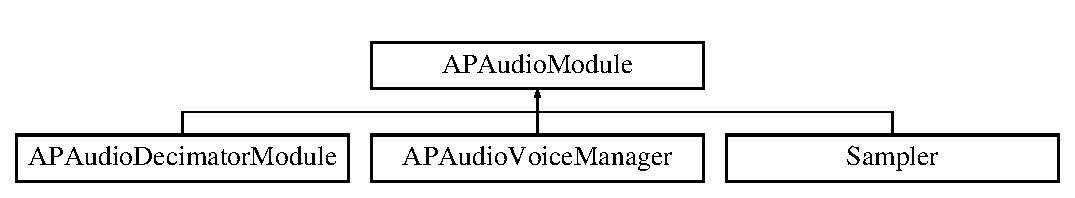
\includegraphics[height=2.000000cm]{class_a_p_audio_module}
\end{center}
\end{figure}
\subsection*{Public Member Functions}
\begin{DoxyCompactItemize}
\item 
\hyperlink{class_a_p_audio_module_ae539348edfb31d1ecaa0e1feb771f901}{A\+P\+Audio\+Module} (\hyperlink{class_a_p_audio_main_frame}{A\+P\+Audio\+Main\+Frame} $\ast$mf)
\item 
virtual \hyperlink{class_a_p_audio_module_af9f5e6f6ff795a4f8218addb0d17aa94}{$\sim$\+A\+P\+Audio\+Module} ()
\item 
virtual void \hyperlink{class_a_p_audio_module_a10c6d7f469b9d1626a80c4d745663a2a}{calculate\+Buffer} ()
\item 
void \hyperlink{class_a_p_audio_module_a2d53c525276aa2876b188b10eb42795f}{set\+I\+D} (juce\+::\+String I\+D)
\item 
juce\+::\+String \hyperlink{class_a_p_audio_module_a8fc7b1e3961d42e8b42a6025ad2181a0}{get\+I\+D} ()
\item 
\hyperlink{_a_p_audio_module_8h_a4ee69c206c9c7015dc653f7e716c4fe8}{Sample} \hyperlink{class_a_p_audio_module_ac4818c202ad9a769773fdad806187cd2}{return\+Output\+Sample} (\hyperlink{_a_p_audio_module_8h_a7d836cc51adbed3f66d5c4c91ed72e94}{Timer\+Value} index)
\item 
void \hyperlink{class_a_p_audio_module_a746277d94090c0d90d5993a3a9a4a533}{connect} (\hyperlink{class_a_p_audio_module}{A\+P\+Audio\+Module} $\ast$module)
\item 
\hyperlink{_a_p_audio_module_8h_a4ee69c206c9c7015dc653f7e716c4fe8}{Sample} \hyperlink{class_a_p_audio_module_af7d8f2e41de7b9cae9a74bba8ebb1fb0}{get\+Sample\+Rate} ()
\item 
\hyperlink{_a_p_audio_module_8h_a7d836cc51adbed3f66d5c4c91ed72e94}{Timer\+Value} \hyperlink{class_a_p_audio_module_a20c96272ef41b2f5b6cc026e58d0b655}{get\+Buffer\+Size} ()
\end{DoxyCompactItemize}
\subsection*{Public Attributes}
\begin{DoxyCompactItemize}
\item 
std\+::vector$<$ \hyperlink{_a_p_audio_module_8h_a4ee69c206c9c7015dc653f7e716c4fe8}{Sample} $>$ \hyperlink{class_a_p_audio_module_a0f04ade4003f1ba68bd1860306d64ffd}{output\+Buffer}
\item 
std\+::vector$<$ \hyperlink{class_a_p_audio_module}{A\+P\+Audio\+Module} $\ast$ $>$ \hyperlink{class_a_p_audio_module_ac702040bf8bdbd10a838e69e2e52845b}{input\+List}
\item 
std\+::vector$<$ \hyperlink{class_a_p_audio_parameter}{A\+P\+Audio\+Parameter} $\ast$ $>$ \hyperlink{class_a_p_audio_module_a87a79681a3f815fa989a03e1f72721a6}{parameters}
\end{DoxyCompactItemize}


\subsection{Constructor \& Destructor Documentation}
\hypertarget{class_a_p_audio_module_ae539348edfb31d1ecaa0e1feb771f901}{\index{A\+P\+Audio\+Module@{A\+P\+Audio\+Module}!A\+P\+Audio\+Module@{A\+P\+Audio\+Module}}
\index{A\+P\+Audio\+Module@{A\+P\+Audio\+Module}!A\+P\+Audio\+Module@{A\+P\+Audio\+Module}}
\subsubsection[{A\+P\+Audio\+Module}]{\setlength{\rightskip}{0pt plus 5cm}A\+P\+Audio\+Module\+::\+A\+P\+Audio\+Module (
\begin{DoxyParamCaption}
\item[{{\bf A\+P\+Audio\+Main\+Frame} $\ast$}]{mf}
\end{DoxyParamCaption}
)}}\label{class_a_p_audio_module_ae539348edfb31d1ecaa0e1feb771f901}
\hypertarget{class_a_p_audio_module_af9f5e6f6ff795a4f8218addb0d17aa94}{\index{A\+P\+Audio\+Module@{A\+P\+Audio\+Module}!````~A\+P\+Audio\+Module@{$\sim$\+A\+P\+Audio\+Module}}
\index{````~A\+P\+Audio\+Module@{$\sim$\+A\+P\+Audio\+Module}!A\+P\+Audio\+Module@{A\+P\+Audio\+Module}}
\subsubsection[{$\sim$\+A\+P\+Audio\+Module}]{\setlength{\rightskip}{0pt plus 5cm}A\+P\+Audio\+Module\+::$\sim$\+A\+P\+Audio\+Module (
\begin{DoxyParamCaption}
{}
\end{DoxyParamCaption}
)\hspace{0.3cm}{\ttfamily [virtual]}}}\label{class_a_p_audio_module_af9f5e6f6ff795a4f8218addb0d17aa94}


\subsection{Member Function Documentation}
\hypertarget{class_a_p_audio_module_a10c6d7f469b9d1626a80c4d745663a2a}{\index{A\+P\+Audio\+Module@{A\+P\+Audio\+Module}!calculate\+Buffer@{calculate\+Buffer}}
\index{calculate\+Buffer@{calculate\+Buffer}!A\+P\+Audio\+Module@{A\+P\+Audio\+Module}}
\subsubsection[{calculate\+Buffer}]{\setlength{\rightskip}{0pt plus 5cm}void A\+P\+Audio\+Module\+::calculate\+Buffer (
\begin{DoxyParamCaption}
{}
\end{DoxyParamCaption}
)\hspace{0.3cm}{\ttfamily [virtual]}}}\label{class_a_p_audio_module_a10c6d7f469b9d1626a80c4d745663a2a}


Reimplemented in \hyperlink{class_a_p_audio_voice_manager_a27033002e3ab86c55ec5d1e5150d1892}{A\+P\+Audio\+Voice\+Manager}, \hyperlink{class_sampler_a1229142ba0a49229553e2cf1a525274d}{Sampler}, and \hyperlink{class_a_p_audio_decimator_module_aeb5165253ed1286fd5a545150a016aae}{A\+P\+Audio\+Decimator\+Module}.

\hypertarget{class_a_p_audio_module_a746277d94090c0d90d5993a3a9a4a533}{\index{A\+P\+Audio\+Module@{A\+P\+Audio\+Module}!connect@{connect}}
\index{connect@{connect}!A\+P\+Audio\+Module@{A\+P\+Audio\+Module}}
\subsubsection[{connect}]{\setlength{\rightskip}{0pt plus 5cm}void A\+P\+Audio\+Module\+::connect (
\begin{DoxyParamCaption}
\item[{{\bf A\+P\+Audio\+Module} $\ast$}]{module}
\end{DoxyParamCaption}
)}}\label{class_a_p_audio_module_a746277d94090c0d90d5993a3a9a4a533}
\hypertarget{class_a_p_audio_module_a20c96272ef41b2f5b6cc026e58d0b655}{\index{A\+P\+Audio\+Module@{A\+P\+Audio\+Module}!get\+Buffer\+Size@{get\+Buffer\+Size}}
\index{get\+Buffer\+Size@{get\+Buffer\+Size}!A\+P\+Audio\+Module@{A\+P\+Audio\+Module}}
\subsubsection[{get\+Buffer\+Size}]{\setlength{\rightskip}{0pt plus 5cm}{\bf Timer\+Value} A\+P\+Audio\+Module\+::get\+Buffer\+Size (
\begin{DoxyParamCaption}
{}
\end{DoxyParamCaption}
)\hspace{0.3cm}{\ttfamily [inline]}}}\label{class_a_p_audio_module_a20c96272ef41b2f5b6cc026e58d0b655}
\hypertarget{class_a_p_audio_module_a8fc7b1e3961d42e8b42a6025ad2181a0}{\index{A\+P\+Audio\+Module@{A\+P\+Audio\+Module}!get\+I\+D@{get\+I\+D}}
\index{get\+I\+D@{get\+I\+D}!A\+P\+Audio\+Module@{A\+P\+Audio\+Module}}
\subsubsection[{get\+I\+D}]{\setlength{\rightskip}{0pt plus 5cm}juce\+::\+String A\+P\+Audio\+Module\+::get\+I\+D (
\begin{DoxyParamCaption}
{}
\end{DoxyParamCaption}
)\hspace{0.3cm}{\ttfamily [inline]}}}\label{class_a_p_audio_module_a8fc7b1e3961d42e8b42a6025ad2181a0}
\hypertarget{class_a_p_audio_module_af7d8f2e41de7b9cae9a74bba8ebb1fb0}{\index{A\+P\+Audio\+Module@{A\+P\+Audio\+Module}!get\+Sample\+Rate@{get\+Sample\+Rate}}
\index{get\+Sample\+Rate@{get\+Sample\+Rate}!A\+P\+Audio\+Module@{A\+P\+Audio\+Module}}
\subsubsection[{get\+Sample\+Rate}]{\setlength{\rightskip}{0pt plus 5cm}{\bf Sample} A\+P\+Audio\+Module\+::get\+Sample\+Rate (
\begin{DoxyParamCaption}
{}
\end{DoxyParamCaption}
)\hspace{0.3cm}{\ttfamily [inline]}}}\label{class_a_p_audio_module_af7d8f2e41de7b9cae9a74bba8ebb1fb0}
\hypertarget{class_a_p_audio_module_ac4818c202ad9a769773fdad806187cd2}{\index{A\+P\+Audio\+Module@{A\+P\+Audio\+Module}!return\+Output\+Sample@{return\+Output\+Sample}}
\index{return\+Output\+Sample@{return\+Output\+Sample}!A\+P\+Audio\+Module@{A\+P\+Audio\+Module}}
\subsubsection[{return\+Output\+Sample}]{\setlength{\rightskip}{0pt plus 5cm}{\bf Sample} A\+P\+Audio\+Module\+::return\+Output\+Sample (
\begin{DoxyParamCaption}
\item[{{\bf Timer\+Value}}]{index}
\end{DoxyParamCaption}
)}}\label{class_a_p_audio_module_ac4818c202ad9a769773fdad806187cd2}
\hypertarget{class_a_p_audio_module_a2d53c525276aa2876b188b10eb42795f}{\index{A\+P\+Audio\+Module@{A\+P\+Audio\+Module}!set\+I\+D@{set\+I\+D}}
\index{set\+I\+D@{set\+I\+D}!A\+P\+Audio\+Module@{A\+P\+Audio\+Module}}
\subsubsection[{set\+I\+D}]{\setlength{\rightskip}{0pt plus 5cm}void A\+P\+Audio\+Module\+::set\+I\+D (
\begin{DoxyParamCaption}
\item[{juce\+::\+String}]{I\+D}
\end{DoxyParamCaption}
)}}\label{class_a_p_audio_module_a2d53c525276aa2876b188b10eb42795f}


\subsection{Member Data Documentation}
\hypertarget{class_a_p_audio_module_ac702040bf8bdbd10a838e69e2e52845b}{\index{A\+P\+Audio\+Module@{A\+P\+Audio\+Module}!input\+List@{input\+List}}
\index{input\+List@{input\+List}!A\+P\+Audio\+Module@{A\+P\+Audio\+Module}}
\subsubsection[{input\+List}]{\setlength{\rightskip}{0pt plus 5cm}std\+::vector$<${\bf A\+P\+Audio\+Module}$\ast$$>$ A\+P\+Audio\+Module\+::input\+List}}\label{class_a_p_audio_module_ac702040bf8bdbd10a838e69e2e52845b}
\hypertarget{class_a_p_audio_module_a0f04ade4003f1ba68bd1860306d64ffd}{\index{A\+P\+Audio\+Module@{A\+P\+Audio\+Module}!output\+Buffer@{output\+Buffer}}
\index{output\+Buffer@{output\+Buffer}!A\+P\+Audio\+Module@{A\+P\+Audio\+Module}}
\subsubsection[{output\+Buffer}]{\setlength{\rightskip}{0pt plus 5cm}std\+::vector$<${\bf Sample}$>$ A\+P\+Audio\+Module\+::output\+Buffer}}\label{class_a_p_audio_module_a0f04ade4003f1ba68bd1860306d64ffd}
\hypertarget{class_a_p_audio_module_a87a79681a3f815fa989a03e1f72721a6}{\index{A\+P\+Audio\+Module@{A\+P\+Audio\+Module}!parameters@{parameters}}
\index{parameters@{parameters}!A\+P\+Audio\+Module@{A\+P\+Audio\+Module}}
\subsubsection[{parameters}]{\setlength{\rightskip}{0pt plus 5cm}std\+::vector$<${\bf A\+P\+Audio\+Parameter}$\ast$$>$ A\+P\+Audio\+Module\+::parameters}}\label{class_a_p_audio_module_a87a79681a3f815fa989a03e1f72721a6}


The documentation for this class was generated from the following files\+:\begin{DoxyCompactItemize}
\item 
Audio Classes/\+Headers/\hyperlink{_a_p_audio_module_8h}{A\+P\+Audio\+Module.\+h}\item 
Audio Classes/\+Implementations/\hyperlink{_a_p_audio_module_8cpp}{A\+P\+Audio\+Module.\+cpp}\end{DoxyCompactItemize}

\hypertarget{class_a_p_audio_parameter}{\section{A\+P\+Audio\+Parameter Class Reference}
\label{class_a_p_audio_parameter}\index{A\+P\+Audio\+Parameter@{A\+P\+Audio\+Parameter}}
}


{\ttfamily \#include $<$A\+P\+Audio\+Parameter.\+h$>$}

\subsection*{Public Member Functions}
\begin{DoxyCompactItemize}
\item 
\hyperlink{class_a_p_audio_parameter_a307626b492f446520333c717d06d1718}{A\+P\+Audio\+Parameter} (\hyperlink{_a_p_audio_module_8h_a9219378a2632ccf0389d00317ce8cdc4}{Control\+Value} min, \hyperlink{_a_p_audio_module_8h_a9219378a2632ccf0389d00317ce8cdc4}{Control\+Value} max, \hyperlink{_a_p_audio_module_8h_a9219378a2632ccf0389d00317ce8cdc4}{Control\+Value} start, juce\+::\+String identification)
\item 
void \hyperlink{class_a_p_audio_parameter_a86fcc968ae6bd3c7cea44e29b4e1ad77}{set\+Min\+Value} (\hyperlink{_a_p_audio_module_8h_a9219378a2632ccf0389d00317ce8cdc4}{Control\+Value} value)
\item 
void \hyperlink{class_a_p_audio_parameter_ac1d7f5d9c8fc15f2f7f793bf9be9e5af}{set\+Max\+Value} (\hyperlink{_a_p_audio_module_8h_a9219378a2632ccf0389d00317ce8cdc4}{Control\+Value} value)
\item 
void \hyperlink{class_a_p_audio_parameter_a40800bb5d6a0bca6cfa75e2dd384d5ea}{set\+Value} (\hyperlink{_a_p_audio_module_8h_a9219378a2632ccf0389d00317ce8cdc4}{Control\+Value} value)
\item 
\hyperlink{_a_p_audio_module_8h_a9219378a2632ccf0389d00317ce8cdc4}{Control\+Value} \hyperlink{class_a_p_audio_parameter_a1704b4d9b97a8d1183cec6bfd5f8c9ec}{get\+Min\+Value} ()
\item 
\hyperlink{_a_p_audio_module_8h_a9219378a2632ccf0389d00317ce8cdc4}{Control\+Value} \hyperlink{class_a_p_audio_parameter_a2a0caf7e8db83f46edb7d184c7c58c08}{get\+Max\+Value} ()
\item 
\hyperlink{_a_p_audio_module_8h_a9219378a2632ccf0389d00317ce8cdc4}{Control\+Value} \hyperlink{class_a_p_audio_parameter_ad017230322b9fe2affaabfe53e83f8c5}{get\+Value} ()
\item 
juce\+::\+String \hyperlink{class_a_p_audio_parameter_a8389ec91a1171892e63e6a9aebee2ace}{get\+I\+D} ()
\end{DoxyCompactItemize}


\subsection{Constructor \& Destructor Documentation}
\hypertarget{class_a_p_audio_parameter_a307626b492f446520333c717d06d1718}{\index{A\+P\+Audio\+Parameter@{A\+P\+Audio\+Parameter}!A\+P\+Audio\+Parameter@{A\+P\+Audio\+Parameter}}
\index{A\+P\+Audio\+Parameter@{A\+P\+Audio\+Parameter}!A\+P\+Audio\+Parameter@{A\+P\+Audio\+Parameter}}
\subsubsection[{A\+P\+Audio\+Parameter}]{\setlength{\rightskip}{0pt plus 5cm}A\+P\+Audio\+Parameter\+::\+A\+P\+Audio\+Parameter (
\begin{DoxyParamCaption}
\item[{{\bf Control\+Value}}]{min, }
\item[{{\bf Control\+Value}}]{max, }
\item[{{\bf Control\+Value}}]{start, }
\item[{juce\+::\+String}]{identification}
\end{DoxyParamCaption}
)}}\label{class_a_p_audio_parameter_a307626b492f446520333c717d06d1718}


\subsection{Member Function Documentation}
\hypertarget{class_a_p_audio_parameter_a8389ec91a1171892e63e6a9aebee2ace}{\index{A\+P\+Audio\+Parameter@{A\+P\+Audio\+Parameter}!get\+I\+D@{get\+I\+D}}
\index{get\+I\+D@{get\+I\+D}!A\+P\+Audio\+Parameter@{A\+P\+Audio\+Parameter}}
\subsubsection[{get\+I\+D}]{\setlength{\rightskip}{0pt plus 5cm}juce\+::\+String A\+P\+Audio\+Parameter\+::get\+I\+D (
\begin{DoxyParamCaption}
{}
\end{DoxyParamCaption}
)\hspace{0.3cm}{\ttfamily [inline]}}}\label{class_a_p_audio_parameter_a8389ec91a1171892e63e6a9aebee2ace}
\hypertarget{class_a_p_audio_parameter_a2a0caf7e8db83f46edb7d184c7c58c08}{\index{A\+P\+Audio\+Parameter@{A\+P\+Audio\+Parameter}!get\+Max\+Value@{get\+Max\+Value}}
\index{get\+Max\+Value@{get\+Max\+Value}!A\+P\+Audio\+Parameter@{A\+P\+Audio\+Parameter}}
\subsubsection[{get\+Max\+Value}]{\setlength{\rightskip}{0pt plus 5cm}{\bf Control\+Value} A\+P\+Audio\+Parameter\+::get\+Max\+Value (
\begin{DoxyParamCaption}
{}
\end{DoxyParamCaption}
)\hspace{0.3cm}{\ttfamily [inline]}}}\label{class_a_p_audio_parameter_a2a0caf7e8db83f46edb7d184c7c58c08}
\hypertarget{class_a_p_audio_parameter_a1704b4d9b97a8d1183cec6bfd5f8c9ec}{\index{A\+P\+Audio\+Parameter@{A\+P\+Audio\+Parameter}!get\+Min\+Value@{get\+Min\+Value}}
\index{get\+Min\+Value@{get\+Min\+Value}!A\+P\+Audio\+Parameter@{A\+P\+Audio\+Parameter}}
\subsubsection[{get\+Min\+Value}]{\setlength{\rightskip}{0pt plus 5cm}{\bf Control\+Value} A\+P\+Audio\+Parameter\+::get\+Min\+Value (
\begin{DoxyParamCaption}
{}
\end{DoxyParamCaption}
)\hspace{0.3cm}{\ttfamily [inline]}}}\label{class_a_p_audio_parameter_a1704b4d9b97a8d1183cec6bfd5f8c9ec}
\hypertarget{class_a_p_audio_parameter_ad017230322b9fe2affaabfe53e83f8c5}{\index{A\+P\+Audio\+Parameter@{A\+P\+Audio\+Parameter}!get\+Value@{get\+Value}}
\index{get\+Value@{get\+Value}!A\+P\+Audio\+Parameter@{A\+P\+Audio\+Parameter}}
\subsubsection[{get\+Value}]{\setlength{\rightskip}{0pt plus 5cm}{\bf Control\+Value} A\+P\+Audio\+Parameter\+::get\+Value (
\begin{DoxyParamCaption}
{}
\end{DoxyParamCaption}
)\hspace{0.3cm}{\ttfamily [inline]}}}\label{class_a_p_audio_parameter_ad017230322b9fe2affaabfe53e83f8c5}
\hypertarget{class_a_p_audio_parameter_ac1d7f5d9c8fc15f2f7f793bf9be9e5af}{\index{A\+P\+Audio\+Parameter@{A\+P\+Audio\+Parameter}!set\+Max\+Value@{set\+Max\+Value}}
\index{set\+Max\+Value@{set\+Max\+Value}!A\+P\+Audio\+Parameter@{A\+P\+Audio\+Parameter}}
\subsubsection[{set\+Max\+Value}]{\setlength{\rightskip}{0pt plus 5cm}void A\+P\+Audio\+Parameter\+::set\+Max\+Value (
\begin{DoxyParamCaption}
\item[{{\bf Control\+Value}}]{value}
\end{DoxyParamCaption}
)}}\label{class_a_p_audio_parameter_ac1d7f5d9c8fc15f2f7f793bf9be9e5af}
\hypertarget{class_a_p_audio_parameter_a86fcc968ae6bd3c7cea44e29b4e1ad77}{\index{A\+P\+Audio\+Parameter@{A\+P\+Audio\+Parameter}!set\+Min\+Value@{set\+Min\+Value}}
\index{set\+Min\+Value@{set\+Min\+Value}!A\+P\+Audio\+Parameter@{A\+P\+Audio\+Parameter}}
\subsubsection[{set\+Min\+Value}]{\setlength{\rightskip}{0pt plus 5cm}void A\+P\+Audio\+Parameter\+::set\+Min\+Value (
\begin{DoxyParamCaption}
\item[{{\bf Control\+Value}}]{value}
\end{DoxyParamCaption}
)}}\label{class_a_p_audio_parameter_a86fcc968ae6bd3c7cea44e29b4e1ad77}
\hypertarget{class_a_p_audio_parameter_a40800bb5d6a0bca6cfa75e2dd384d5ea}{\index{A\+P\+Audio\+Parameter@{A\+P\+Audio\+Parameter}!set\+Value@{set\+Value}}
\index{set\+Value@{set\+Value}!A\+P\+Audio\+Parameter@{A\+P\+Audio\+Parameter}}
\subsubsection[{set\+Value}]{\setlength{\rightskip}{0pt plus 5cm}void A\+P\+Audio\+Parameter\+::set\+Value (
\begin{DoxyParamCaption}
\item[{{\bf Control\+Value}}]{value}
\end{DoxyParamCaption}
)}}\label{class_a_p_audio_parameter_a40800bb5d6a0bca6cfa75e2dd384d5ea}


The documentation for this class was generated from the following files\+:\begin{DoxyCompactItemize}
\item 
Audio Classes/\+Headers/\hyperlink{_a_p_audio_parameter_8h}{A\+P\+Audio\+Parameter.\+h}\item 
Audio Classes/\+Implementations/\hyperlink{_a_p_audio_parameter_8cpp}{A\+P\+Audio\+Parameter.\+cpp}\end{DoxyCompactItemize}

\hypertarget{class_a_p_audio_processor_c_p_p}{\section{A\+P\+Audio\+Processor\+C\+P\+P Class Reference}
\label{class_a_p_audio_processor_c_p_p}\index{A\+P\+Audio\+Processor\+C\+P\+P@{A\+P\+Audio\+Processor\+C\+P\+P}}
}


{\ttfamily \#include $<$A\+P\+Audio\+Processor.\+h$>$}

\subsection*{Public Member Functions}
\begin{DoxyCompactItemize}
\item 
\hyperlink{class_a_p_audio_processor_c_p_p_ab8efea43137a2c221684e61cf68c9dd5}{A\+P\+Audio\+Processor\+C\+P\+P} ()
\item 
virtual void \hyperlink{class_a_p_audio_processor_c_p_p_a17957f60025f94b1abaaa4c9a532402c}{process} (U\+Int16 buffer\+Size, Audio\+Buffer\+List $\ast$buffers)=0
\item 
\hyperlink{_a_p_audio_module_8h_a9219378a2632ccf0389d00317ce8cdc4}{Control\+Value} \hyperlink{class_a_p_audio_processor_c_p_p_a5a3717f7717eeb59ad14f7e08e09438c}{get\+Sample\+Rate} ()
\item 
U\+Int32 \hyperlink{class_a_p_audio_processor_c_p_p_a37fbd4862b2466a69079229be15f1315}{get\+Buffer\+Size} ()
\item 
O\+S\+Status \hyperlink{class_a_p_audio_processor_c_p_p_a9d80b7cc8fe1a7201e6b7602db4022e2}{start\+Processor} ()
\end{DoxyCompactItemize}


\subsection{Constructor \& Destructor Documentation}
\hypertarget{class_a_p_audio_processor_c_p_p_ab8efea43137a2c221684e61cf68c9dd5}{\index{A\+P\+Audio\+Processor\+C\+P\+P@{A\+P\+Audio\+Processor\+C\+P\+P}!A\+P\+Audio\+Processor\+C\+P\+P@{A\+P\+Audio\+Processor\+C\+P\+P}}
\index{A\+P\+Audio\+Processor\+C\+P\+P@{A\+P\+Audio\+Processor\+C\+P\+P}!A\+P\+Audio\+Processor\+C\+P\+P@{A\+P\+Audio\+Processor\+C\+P\+P}}
\subsubsection[{A\+P\+Audio\+Processor\+C\+P\+P}]{\setlength{\rightskip}{0pt plus 5cm}A\+P\+Audio\+Processor\+C\+P\+P\+::\+A\+P\+Audio\+Processor\+C\+P\+P (
\begin{DoxyParamCaption}
{}
\end{DoxyParamCaption}
)}}\label{class_a_p_audio_processor_c_p_p_ab8efea43137a2c221684e61cf68c9dd5}


\subsection{Member Function Documentation}
\hypertarget{class_a_p_audio_processor_c_p_p_a37fbd4862b2466a69079229be15f1315}{\index{A\+P\+Audio\+Processor\+C\+P\+P@{A\+P\+Audio\+Processor\+C\+P\+P}!get\+Buffer\+Size@{get\+Buffer\+Size}}
\index{get\+Buffer\+Size@{get\+Buffer\+Size}!A\+P\+Audio\+Processor\+C\+P\+P@{A\+P\+Audio\+Processor\+C\+P\+P}}
\subsubsection[{get\+Buffer\+Size}]{\setlength{\rightskip}{0pt plus 5cm}U\+Int32 A\+P\+Audio\+Processor\+C\+P\+P\+::get\+Buffer\+Size (
\begin{DoxyParamCaption}
{}
\end{DoxyParamCaption}
)\hspace{0.3cm}{\ttfamily [inline]}}}\label{class_a_p_audio_processor_c_p_p_a37fbd4862b2466a69079229be15f1315}
\hypertarget{class_a_p_audio_processor_c_p_p_a5a3717f7717eeb59ad14f7e08e09438c}{\index{A\+P\+Audio\+Processor\+C\+P\+P@{A\+P\+Audio\+Processor\+C\+P\+P}!get\+Sample\+Rate@{get\+Sample\+Rate}}
\index{get\+Sample\+Rate@{get\+Sample\+Rate}!A\+P\+Audio\+Processor\+C\+P\+P@{A\+P\+Audio\+Processor\+C\+P\+P}}
\subsubsection[{get\+Sample\+Rate}]{\setlength{\rightskip}{0pt plus 5cm}{\bf Control\+Value} A\+P\+Audio\+Processor\+C\+P\+P\+::get\+Sample\+Rate (
\begin{DoxyParamCaption}
{}
\end{DoxyParamCaption}
)\hspace{0.3cm}{\ttfamily [inline]}}}\label{class_a_p_audio_processor_c_p_p_a5a3717f7717eeb59ad14f7e08e09438c}
\hypertarget{class_a_p_audio_processor_c_p_p_a17957f60025f94b1abaaa4c9a532402c}{\index{A\+P\+Audio\+Processor\+C\+P\+P@{A\+P\+Audio\+Processor\+C\+P\+P}!process@{process}}
\index{process@{process}!A\+P\+Audio\+Processor\+C\+P\+P@{A\+P\+Audio\+Processor\+C\+P\+P}}
\subsubsection[{process}]{\setlength{\rightskip}{0pt plus 5cm}virtual void A\+P\+Audio\+Processor\+C\+P\+P\+::process (
\begin{DoxyParamCaption}
\item[{U\+Int16}]{buffer\+Size, }
\item[{Audio\+Buffer\+List $\ast$}]{buffers}
\end{DoxyParamCaption}
)\hspace{0.3cm}{\ttfamily [pure virtual]}}}\label{class_a_p_audio_processor_c_p_p_a17957f60025f94b1abaaa4c9a532402c}
\hypertarget{class_a_p_audio_processor_c_p_p_a9d80b7cc8fe1a7201e6b7602db4022e2}{\index{A\+P\+Audio\+Processor\+C\+P\+P@{A\+P\+Audio\+Processor\+C\+P\+P}!start\+Processor@{start\+Processor}}
\index{start\+Processor@{start\+Processor}!A\+P\+Audio\+Processor\+C\+P\+P@{A\+P\+Audio\+Processor\+C\+P\+P}}
\subsubsection[{start\+Processor}]{\setlength{\rightskip}{0pt plus 5cm}O\+S\+Status A\+P\+Audio\+Processor\+C\+P\+P\+::start\+Processor (
\begin{DoxyParamCaption}
{}
\end{DoxyParamCaption}
)}}\label{class_a_p_audio_processor_c_p_p_a9d80b7cc8fe1a7201e6b7602db4022e2}


The documentation for this class was generated from the following files\+:\begin{DoxyCompactItemize}
\item 
In Development (don't include)/\hyperlink{_a_p_audio_processor_8h}{A\+P\+Audio\+Processor.\+h}\item 
In Development (don't include)/\hyperlink{_a_p_audio_processor_8cpp}{A\+P\+Audio\+Processor.\+cpp}\end{DoxyCompactItemize}

\hypertarget{class_a_p_audio_sampler_voice}{\section{A\+P\+Audio\+Sampler\+Voice Class Reference}
\label{class_a_p_audio_sampler_voice}\index{A\+P\+Audio\+Sampler\+Voice@{A\+P\+Audio\+Sampler\+Voice}}
}


{\ttfamily \#include $<$A\+P\+Audio\+Sampler\+Voice.\+h$>$}

Inheritance diagram for A\+P\+Audio\+Sampler\+Voice\+:\begin{figure}[H]
\begin{center}
\leavevmode
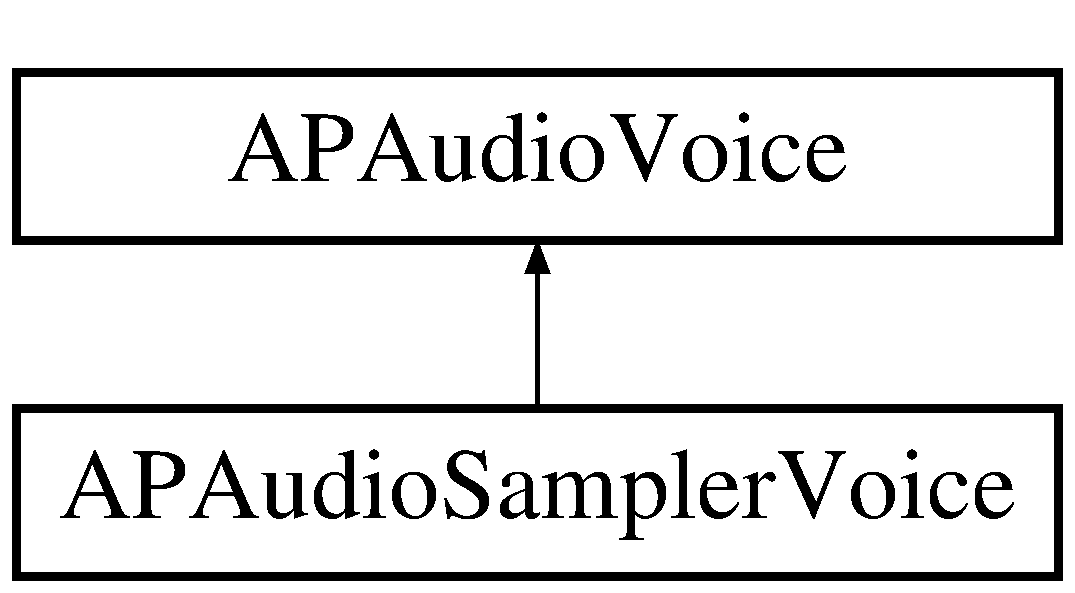
\includegraphics[height=2.000000cm]{class_a_p_audio_sampler_voice}
\end{center}
\end{figure}
\subsection*{Public Member Functions}
\begin{DoxyCompactItemize}
\item 
\hyperlink{class_a_p_audio_sampler_voice_a6ac63a6c78e0e581b5a5b7ab5aa8dc6c}{A\+P\+Audio\+Sampler\+Voice} ()
\item 
void \hyperlink{class_a_p_audio_sampler_voice_ac0a8118282d9e2edf695c6c3c683eac0}{play} (bool repeat)
\item 
bool \hyperlink{class_a_p_audio_sampler_voice_a8f0b92e13673db88b65411d03368f5a6}{is\+Playing} ()
\item 
float \hyperlink{class_a_p_audio_sampler_voice_a54a619f1d79b8ec8026a59865736100c}{tick} ()
\item 
void \hyperlink{class_a_p_audio_sampler_voice_a20cb748c04da47d05810393c8cc7af27}{set\+File\+To\+Play} (\hyperlink{class_a_p_audio_file}{A\+P\+Audio\+File} $\ast$file\+To\+Play)
\item 
void \hyperlink{class_a_p_audio_sampler_voice_a77f7d566474366f142f1782305e1df60}{set\+Speed} (float speed)
\item 
void \hyperlink{class_a_p_audio_sampler_voice_a6d56d1517396372a76a06efc98c81095}{set\+Amplitude} (float amp)
\item 
void \hyperlink{class_a_p_audio_sampler_voice_a9cca9818b0ed91df459e3ac6fdbe4ba3}{set\+Note} (int note)
\item 
int \hyperlink{class_a_p_audio_sampler_voice_ae596fdf1bd14a35a18cd3d61761301c3}{get\+Note} ()
\item 
\hyperlink{class_a_p_audio_sampler_voice_a6ac63a6c78e0e581b5a5b7ab5aa8dc6c}{A\+P\+Audio\+Sampler\+Voice} ()
\item 
void \hyperlink{class_a_p_audio_sampler_voice_a2771cb306e331a458cea4283048c374c}{render\+Next\+Block} (\hyperlink{_a_p_audio_module_8h_a2c2f997fdc6b0e88b3723fb20dc502f0}{Sample\+Buffer} output\+Buffer, int start\+Sample, int num\+Samples, \hyperlink{_a_p_audio_module_8h_a9cc0620fb2e91b51587c6936060d4161}{U\+Int} channel) override
\item 
void \hyperlink{class_a_p_audio_sampler_voice_af251bd2529b4472729db61d54753cc56}{stop\+Voice} () override
\item 
bool \hyperlink{class_a_p_audio_sampler_voice_af9959b4be2689341d32e697b5cef7ab5}{can\+Play\+Sound} (\hyperlink{class_a_p_audio_sound_description}{A\+P\+Audio\+Sound\+Description} $\ast$sound) override
\item 
void \hyperlink{class_a_p_audio_sampler_voice_acc47dbbd5d5835092c4806d245c53188}{reset} () override
\end{DoxyCompactItemize}


\subsection{Constructor \& Destructor Documentation}
\hypertarget{class_a_p_audio_sampler_voice_a6ac63a6c78e0e581b5a5b7ab5aa8dc6c}{\index{A\+P\+Audio\+Sampler\+Voice@{A\+P\+Audio\+Sampler\+Voice}!A\+P\+Audio\+Sampler\+Voice@{A\+P\+Audio\+Sampler\+Voice}}
\index{A\+P\+Audio\+Sampler\+Voice@{A\+P\+Audio\+Sampler\+Voice}!A\+P\+Audio\+Sampler\+Voice@{A\+P\+Audio\+Sampler\+Voice}}
\subsubsection[{A\+P\+Audio\+Sampler\+Voice}]{\setlength{\rightskip}{0pt plus 5cm}A\+P\+Audio\+Sampler\+Voice\+::\+A\+P\+Audio\+Sampler\+Voice (
\begin{DoxyParamCaption}
{}
\end{DoxyParamCaption}
)}}\label{class_a_p_audio_sampler_voice_a6ac63a6c78e0e581b5a5b7ab5aa8dc6c}
\hypertarget{class_a_p_audio_sampler_voice_a6ac63a6c78e0e581b5a5b7ab5aa8dc6c}{\index{A\+P\+Audio\+Sampler\+Voice@{A\+P\+Audio\+Sampler\+Voice}!A\+P\+Audio\+Sampler\+Voice@{A\+P\+Audio\+Sampler\+Voice}}
\index{A\+P\+Audio\+Sampler\+Voice@{A\+P\+Audio\+Sampler\+Voice}!A\+P\+Audio\+Sampler\+Voice@{A\+P\+Audio\+Sampler\+Voice}}
\subsubsection[{A\+P\+Audio\+Sampler\+Voice}]{\setlength{\rightskip}{0pt plus 5cm}A\+P\+Audio\+Sampler\+Voice\+::\+A\+P\+Audio\+Sampler\+Voice (
\begin{DoxyParamCaption}
{}
\end{DoxyParamCaption}
)}}\label{class_a_p_audio_sampler_voice_a6ac63a6c78e0e581b5a5b7ab5aa8dc6c}


\subsection{Member Function Documentation}
\hypertarget{class_a_p_audio_sampler_voice_af9959b4be2689341d32e697b5cef7ab5}{\index{A\+P\+Audio\+Sampler\+Voice@{A\+P\+Audio\+Sampler\+Voice}!can\+Play\+Sound@{can\+Play\+Sound}}
\index{can\+Play\+Sound@{can\+Play\+Sound}!A\+P\+Audio\+Sampler\+Voice@{A\+P\+Audio\+Sampler\+Voice}}
\subsubsection[{can\+Play\+Sound}]{\setlength{\rightskip}{0pt plus 5cm}bool A\+P\+Audio\+Sampler\+Voice\+::can\+Play\+Sound (
\begin{DoxyParamCaption}
\item[{{\bf A\+P\+Audio\+Sound\+Description} $\ast$}]{sound}
\end{DoxyParamCaption}
)\hspace{0.3cm}{\ttfamily [override]}, {\ttfamily [virtual]}}}\label{class_a_p_audio_sampler_voice_af9959b4be2689341d32e697b5cef7ab5}


Implements \hyperlink{class_a_p_audio_voice_a4c534683ad441b5ff7e14ed528e058a4}{A\+P\+Audio\+Voice}.

\hypertarget{class_a_p_audio_sampler_voice_ae596fdf1bd14a35a18cd3d61761301c3}{\index{A\+P\+Audio\+Sampler\+Voice@{A\+P\+Audio\+Sampler\+Voice}!get\+Note@{get\+Note}}
\index{get\+Note@{get\+Note}!A\+P\+Audio\+Sampler\+Voice@{A\+P\+Audio\+Sampler\+Voice}}
\subsubsection[{get\+Note}]{\setlength{\rightskip}{0pt plus 5cm}int A\+P\+Audio\+Sampler\+Voice\+::get\+Note (
\begin{DoxyParamCaption}
{}
\end{DoxyParamCaption}
)}}\label{class_a_p_audio_sampler_voice_ae596fdf1bd14a35a18cd3d61761301c3}
\hypertarget{class_a_p_audio_sampler_voice_a8f0b92e13673db88b65411d03368f5a6}{\index{A\+P\+Audio\+Sampler\+Voice@{A\+P\+Audio\+Sampler\+Voice}!is\+Playing@{is\+Playing}}
\index{is\+Playing@{is\+Playing}!A\+P\+Audio\+Sampler\+Voice@{A\+P\+Audio\+Sampler\+Voice}}
\subsubsection[{is\+Playing}]{\setlength{\rightskip}{0pt plus 5cm}bool A\+P\+Audio\+Sampler\+Voice\+::is\+Playing (
\begin{DoxyParamCaption}
{}
\end{DoxyParamCaption}
)}}\label{class_a_p_audio_sampler_voice_a8f0b92e13673db88b65411d03368f5a6}
\hypertarget{class_a_p_audio_sampler_voice_ac0a8118282d9e2edf695c6c3c683eac0}{\index{A\+P\+Audio\+Sampler\+Voice@{A\+P\+Audio\+Sampler\+Voice}!play@{play}}
\index{play@{play}!A\+P\+Audio\+Sampler\+Voice@{A\+P\+Audio\+Sampler\+Voice}}
\subsubsection[{play}]{\setlength{\rightskip}{0pt plus 5cm}void A\+P\+Audio\+Sampler\+Voice\+::play (
\begin{DoxyParamCaption}
\item[{bool}]{repeat}
\end{DoxyParamCaption}
)}}\label{class_a_p_audio_sampler_voice_ac0a8118282d9e2edf695c6c3c683eac0}
\hypertarget{class_a_p_audio_sampler_voice_a2771cb306e331a458cea4283048c374c}{\index{A\+P\+Audio\+Sampler\+Voice@{A\+P\+Audio\+Sampler\+Voice}!render\+Next\+Block@{render\+Next\+Block}}
\index{render\+Next\+Block@{render\+Next\+Block}!A\+P\+Audio\+Sampler\+Voice@{A\+P\+Audio\+Sampler\+Voice}}
\subsubsection[{render\+Next\+Block}]{\setlength{\rightskip}{0pt plus 5cm}void A\+P\+Audio\+Sampler\+Voice\+::render\+Next\+Block (
\begin{DoxyParamCaption}
\item[{{\bf Sample\+Buffer}}]{output\+Buffer, }
\item[{int}]{start\+Sample, }
\item[{int}]{num\+Samples, }
\item[{{\bf U\+Int}}]{channel}
\end{DoxyParamCaption}
)\hspace{0.3cm}{\ttfamily [override]}, {\ttfamily [virtual]}}}\label{class_a_p_audio_sampler_voice_a2771cb306e331a458cea4283048c374c}


Implements \hyperlink{class_a_p_audio_voice_a151ae804092f9c6b9925f450565e3df4}{A\+P\+Audio\+Voice}.

\hypertarget{class_a_p_audio_sampler_voice_acc47dbbd5d5835092c4806d245c53188}{\index{A\+P\+Audio\+Sampler\+Voice@{A\+P\+Audio\+Sampler\+Voice}!reset@{reset}}
\index{reset@{reset}!A\+P\+Audio\+Sampler\+Voice@{A\+P\+Audio\+Sampler\+Voice}}
\subsubsection[{reset}]{\setlength{\rightskip}{0pt plus 5cm}void A\+P\+Audio\+Sampler\+Voice\+::reset (
\begin{DoxyParamCaption}
{}
\end{DoxyParamCaption}
)\hspace{0.3cm}{\ttfamily [override]}, {\ttfamily [virtual]}}}\label{class_a_p_audio_sampler_voice_acc47dbbd5d5835092c4806d245c53188}


Implements \hyperlink{class_a_p_audio_voice_a9d8807cb399e9d5fb5ce207ab9f89416}{A\+P\+Audio\+Voice}.

\hypertarget{class_a_p_audio_sampler_voice_a6d56d1517396372a76a06efc98c81095}{\index{A\+P\+Audio\+Sampler\+Voice@{A\+P\+Audio\+Sampler\+Voice}!set\+Amplitude@{set\+Amplitude}}
\index{set\+Amplitude@{set\+Amplitude}!A\+P\+Audio\+Sampler\+Voice@{A\+P\+Audio\+Sampler\+Voice}}
\subsubsection[{set\+Amplitude}]{\setlength{\rightskip}{0pt plus 5cm}void A\+P\+Audio\+Sampler\+Voice\+::set\+Amplitude (
\begin{DoxyParamCaption}
\item[{float}]{amp}
\end{DoxyParamCaption}
)}}\label{class_a_p_audio_sampler_voice_a6d56d1517396372a76a06efc98c81095}
\hypertarget{class_a_p_audio_sampler_voice_a20cb748c04da47d05810393c8cc7af27}{\index{A\+P\+Audio\+Sampler\+Voice@{A\+P\+Audio\+Sampler\+Voice}!set\+File\+To\+Play@{set\+File\+To\+Play}}
\index{set\+File\+To\+Play@{set\+File\+To\+Play}!A\+P\+Audio\+Sampler\+Voice@{A\+P\+Audio\+Sampler\+Voice}}
\subsubsection[{set\+File\+To\+Play}]{\setlength{\rightskip}{0pt plus 5cm}void A\+P\+Audio\+Sampler\+Voice\+::set\+File\+To\+Play (
\begin{DoxyParamCaption}
\item[{{\bf A\+P\+Audio\+File} $\ast$}]{file\+To\+Play}
\end{DoxyParamCaption}
)}}\label{class_a_p_audio_sampler_voice_a20cb748c04da47d05810393c8cc7af27}
\hypertarget{class_a_p_audio_sampler_voice_a9cca9818b0ed91df459e3ac6fdbe4ba3}{\index{A\+P\+Audio\+Sampler\+Voice@{A\+P\+Audio\+Sampler\+Voice}!set\+Note@{set\+Note}}
\index{set\+Note@{set\+Note}!A\+P\+Audio\+Sampler\+Voice@{A\+P\+Audio\+Sampler\+Voice}}
\subsubsection[{set\+Note}]{\setlength{\rightskip}{0pt plus 5cm}void A\+P\+Audio\+Sampler\+Voice\+::set\+Note (
\begin{DoxyParamCaption}
\item[{int}]{note}
\end{DoxyParamCaption}
)}}\label{class_a_p_audio_sampler_voice_a9cca9818b0ed91df459e3ac6fdbe4ba3}
\hypertarget{class_a_p_audio_sampler_voice_a77f7d566474366f142f1782305e1df60}{\index{A\+P\+Audio\+Sampler\+Voice@{A\+P\+Audio\+Sampler\+Voice}!set\+Speed@{set\+Speed}}
\index{set\+Speed@{set\+Speed}!A\+P\+Audio\+Sampler\+Voice@{A\+P\+Audio\+Sampler\+Voice}}
\subsubsection[{set\+Speed}]{\setlength{\rightskip}{0pt plus 5cm}void A\+P\+Audio\+Sampler\+Voice\+::set\+Speed (
\begin{DoxyParamCaption}
\item[{float}]{speed}
\end{DoxyParamCaption}
)}}\label{class_a_p_audio_sampler_voice_a77f7d566474366f142f1782305e1df60}
\hypertarget{class_a_p_audio_sampler_voice_af251bd2529b4472729db61d54753cc56}{\index{A\+P\+Audio\+Sampler\+Voice@{A\+P\+Audio\+Sampler\+Voice}!stop\+Voice@{stop\+Voice}}
\index{stop\+Voice@{stop\+Voice}!A\+P\+Audio\+Sampler\+Voice@{A\+P\+Audio\+Sampler\+Voice}}
\subsubsection[{stop\+Voice}]{\setlength{\rightskip}{0pt plus 5cm}void A\+P\+Audio\+Sampler\+Voice\+::stop\+Voice (
\begin{DoxyParamCaption}
{}
\end{DoxyParamCaption}
)\hspace{0.3cm}{\ttfamily [override]}, {\ttfamily [virtual]}}}\label{class_a_p_audio_sampler_voice_af251bd2529b4472729db61d54753cc56}


Implements \hyperlink{class_a_p_audio_voice_a25b0e54f49472f05ccafb38c782faae8}{A\+P\+Audio\+Voice}.

\hypertarget{class_a_p_audio_sampler_voice_a54a619f1d79b8ec8026a59865736100c}{\index{A\+P\+Audio\+Sampler\+Voice@{A\+P\+Audio\+Sampler\+Voice}!tick@{tick}}
\index{tick@{tick}!A\+P\+Audio\+Sampler\+Voice@{A\+P\+Audio\+Sampler\+Voice}}
\subsubsection[{tick}]{\setlength{\rightskip}{0pt plus 5cm}float A\+P\+Audio\+Sampler\+Voice\+::tick (
\begin{DoxyParamCaption}
{}
\end{DoxyParamCaption}
)}}\label{class_a_p_audio_sampler_voice_a54a619f1d79b8ec8026a59865736100c}


The documentation for this class was generated from the following files\+:\begin{DoxyCompactItemize}
\item 
Audio Classes/\+Headers/\hyperlink{_audio_01_classes_2_headers_2_a_p_audio_sampler_voice_8h}{A\+P\+Audio\+Sampler\+Voice.\+h}\item 
Audio Classes/\+Implementations/\hyperlink{_audio_01_classes_2_implementations_2_a_p_audio_sampler_voice_8cpp}{A\+P\+Audio\+Sampler\+Voice.\+cpp}\end{DoxyCompactItemize}

\hypertarget{class_a_p_audio_sample_sound}{\section{A\+P\+Audio\+Sample\+Sound Class Reference}
\label{class_a_p_audio_sample_sound}\index{A\+P\+Audio\+Sample\+Sound@{A\+P\+Audio\+Sample\+Sound}}
}


{\ttfamily \#include $<$A\+P\+Audio\+Sample\+Sound.\+h$>$}

Inheritance diagram for A\+P\+Audio\+Sample\+Sound\+:\begin{figure}[H]
\begin{center}
\leavevmode
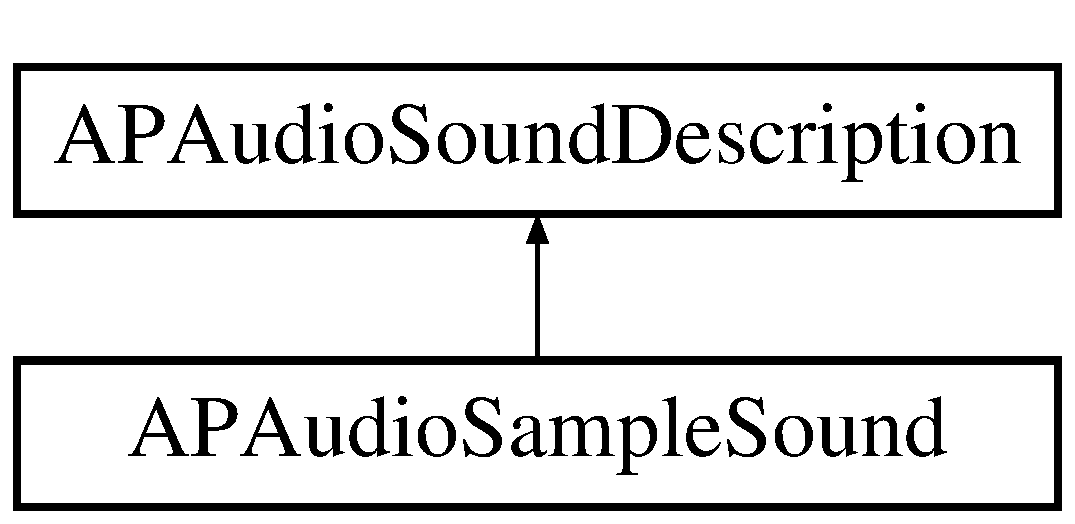
\includegraphics[height=2.000000cm]{class_a_p_audio_sample_sound}
\end{center}
\end{figure}
\subsection*{Public Member Functions}
\begin{DoxyCompactItemize}
\item 
\hyperlink{class_a_p_audio_sample_sound_a2e67be5d19815f8ad292a1622deb522e}{A\+P\+Audio\+Sample\+Sound} ()
\item 
virtual \hyperlink{class_a_p_audio_sample_sound_ad791ba969a5f25573252e893d9bcbdcc}{$\sim$\+A\+P\+Audio\+Sample\+Sound} ()
\item 
bool \hyperlink{class_a_p_audio_sample_sound_a08d23ea13830a9251d638c77b5426e0d}{listens\+To\+Note} (\hyperlink{_a_p_audio_module_8h_a9219378a2632ccf0389d00317ce8cdc4}{Control\+Value} note) override
\item 
bool \hyperlink{class_a_p_audio_sample_sound_a7498818340851d93745bc0d4946532f3}{listens\+To\+Channel} (\hyperlink{_a_p_audio_module_8h_a9219378a2632ccf0389d00317ce8cdc4}{Control\+Value} channel) override
\end{DoxyCompactItemize}


\subsection{Constructor \& Destructor Documentation}
\hypertarget{class_a_p_audio_sample_sound_a2e67be5d19815f8ad292a1622deb522e}{\index{A\+P\+Audio\+Sample\+Sound@{A\+P\+Audio\+Sample\+Sound}!A\+P\+Audio\+Sample\+Sound@{A\+P\+Audio\+Sample\+Sound}}
\index{A\+P\+Audio\+Sample\+Sound@{A\+P\+Audio\+Sample\+Sound}!A\+P\+Audio\+Sample\+Sound@{A\+P\+Audio\+Sample\+Sound}}
\subsubsection[{A\+P\+Audio\+Sample\+Sound}]{\setlength{\rightskip}{0pt plus 5cm}A\+P\+Audio\+Sample\+Sound\+::\+A\+P\+Audio\+Sample\+Sound (
\begin{DoxyParamCaption}
{}
\end{DoxyParamCaption}
)}}\label{class_a_p_audio_sample_sound_a2e67be5d19815f8ad292a1622deb522e}
\hypertarget{class_a_p_audio_sample_sound_ad791ba969a5f25573252e893d9bcbdcc}{\index{A\+P\+Audio\+Sample\+Sound@{A\+P\+Audio\+Sample\+Sound}!````~A\+P\+Audio\+Sample\+Sound@{$\sim$\+A\+P\+Audio\+Sample\+Sound}}
\index{````~A\+P\+Audio\+Sample\+Sound@{$\sim$\+A\+P\+Audio\+Sample\+Sound}!A\+P\+Audio\+Sample\+Sound@{A\+P\+Audio\+Sample\+Sound}}
\subsubsection[{$\sim$\+A\+P\+Audio\+Sample\+Sound}]{\setlength{\rightskip}{0pt plus 5cm}A\+P\+Audio\+Sample\+Sound\+::$\sim$\+A\+P\+Audio\+Sample\+Sound (
\begin{DoxyParamCaption}
{}
\end{DoxyParamCaption}
)\hspace{0.3cm}{\ttfamily [virtual]}}}\label{class_a_p_audio_sample_sound_ad791ba969a5f25573252e893d9bcbdcc}


\subsection{Member Function Documentation}
\hypertarget{class_a_p_audio_sample_sound_a7498818340851d93745bc0d4946532f3}{\index{A\+P\+Audio\+Sample\+Sound@{A\+P\+Audio\+Sample\+Sound}!listens\+To\+Channel@{listens\+To\+Channel}}
\index{listens\+To\+Channel@{listens\+To\+Channel}!A\+P\+Audio\+Sample\+Sound@{A\+P\+Audio\+Sample\+Sound}}
\subsubsection[{listens\+To\+Channel}]{\setlength{\rightskip}{0pt plus 5cm}bool A\+P\+Audio\+Sample\+Sound\+::listens\+To\+Channel (
\begin{DoxyParamCaption}
\item[{{\bf Control\+Value}}]{channel}
\end{DoxyParamCaption}
)\hspace{0.3cm}{\ttfamily [override]}, {\ttfamily [virtual]}}}\label{class_a_p_audio_sample_sound_a7498818340851d93745bc0d4946532f3}


Implements \hyperlink{class_a_p_audio_sound_description_aa4ab161259b35de895c07eb718629b98}{A\+P\+Audio\+Sound\+Description}.

\hypertarget{class_a_p_audio_sample_sound_a08d23ea13830a9251d638c77b5426e0d}{\index{A\+P\+Audio\+Sample\+Sound@{A\+P\+Audio\+Sample\+Sound}!listens\+To\+Note@{listens\+To\+Note}}
\index{listens\+To\+Note@{listens\+To\+Note}!A\+P\+Audio\+Sample\+Sound@{A\+P\+Audio\+Sample\+Sound}}
\subsubsection[{listens\+To\+Note}]{\setlength{\rightskip}{0pt plus 5cm}bool A\+P\+Audio\+Sample\+Sound\+::listens\+To\+Note (
\begin{DoxyParamCaption}
\item[{{\bf Control\+Value}}]{note}
\end{DoxyParamCaption}
)\hspace{0.3cm}{\ttfamily [override]}, {\ttfamily [virtual]}}}\label{class_a_p_audio_sample_sound_a08d23ea13830a9251d638c77b5426e0d}


Implements \hyperlink{class_a_p_audio_sound_description_af0e31cf64b1726fb97c9d027d2bc4c74}{A\+P\+Audio\+Sound\+Description}.



The documentation for this class was generated from the following files\+:\begin{DoxyCompactItemize}
\item 
In Development (don't include)/\hyperlink{_a_p_audio_sample_sound_8h}{A\+P\+Audio\+Sample\+Sound.\+h}\item 
In Development (don't include)/\hyperlink{_a_p_audio_sample_sound_8cpp}{A\+P\+Audio\+Sample\+Sound.\+cpp}\end{DoxyCompactItemize}

\hypertarget{class_a_p_audio_scale_component}{\section{A\+P\+Audio\+Scale\+Component Class Reference}
\label{class_a_p_audio_scale_component}\index{A\+P\+Audio\+Scale\+Component@{A\+P\+Audio\+Scale\+Component}}
}


{\ttfamily \#include $<$A\+P\+Audio\+Scale\+Component.\+h$>$}

Inheritance diagram for A\+P\+Audio\+Scale\+Component\+:\begin{figure}[H]
\begin{center}
\leavevmode
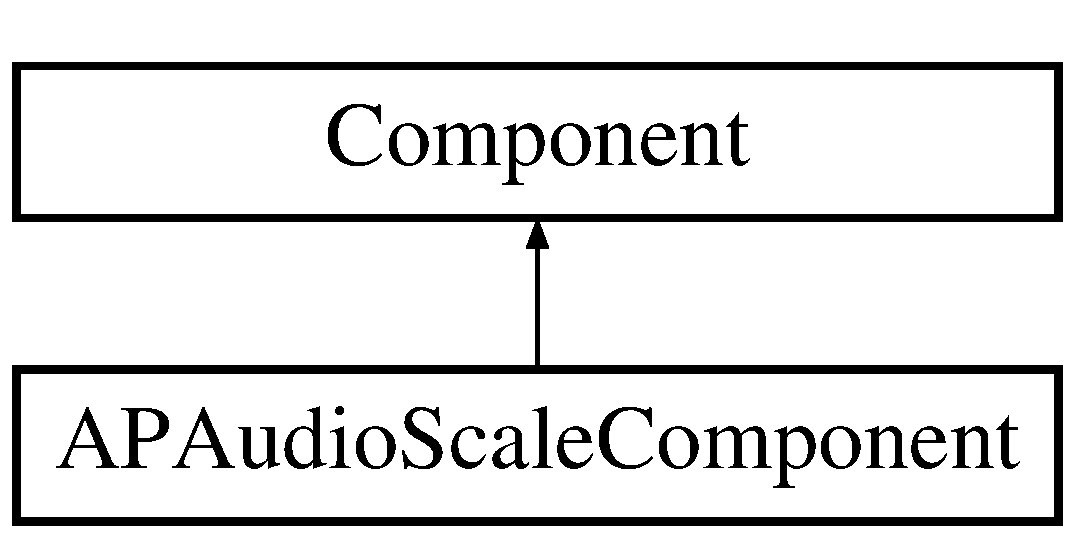
\includegraphics[height=2.000000cm]{class_a_p_audio_scale_component}
\end{center}
\end{figure}
\subsection*{Public Member Functions}
\begin{DoxyCompactItemize}
\item 
\hyperlink{class_a_p_audio_scale_component_ae560d2178f7e2138808dffa9d63a3edc}{A\+P\+Audio\+Scale\+Component} ()
\item 
\hyperlink{class_a_p_audio_scale_component_a84665bd00fef45607e730654d16c2eb1}{$\sim$\+A\+P\+Audio\+Scale\+Component} ()
\item 
void \hyperlink{class_a_p_audio_scale_component_a6ccd9a808d1696121f95920f382247ca}{resized} () overridefinal
\item 
void \hyperlink{class_a_p_audio_scale_component_af4cdde89aad8ed3c4942fafeda46e03c}{paint} (Graphics \&g) overridefinal
\item 
void \hyperlink{class_a_p_audio_scale_component_af252d75f40171dd94349566cc047764d}{set\+Values} (int max, int sample\+Rate)
\item 
void \hyperlink{class_a_p_audio_scale_component_aefe34b461dcf16fb5ddd9307c7f2dcb5}{set\+Zoom} (int zoom)
\end{DoxyCompactItemize}


\subsection{Constructor \& Destructor Documentation}
\hypertarget{class_a_p_audio_scale_component_ae560d2178f7e2138808dffa9d63a3edc}{\index{A\+P\+Audio\+Scale\+Component@{A\+P\+Audio\+Scale\+Component}!A\+P\+Audio\+Scale\+Component@{A\+P\+Audio\+Scale\+Component}}
\index{A\+P\+Audio\+Scale\+Component@{A\+P\+Audio\+Scale\+Component}!A\+P\+Audio\+Scale\+Component@{A\+P\+Audio\+Scale\+Component}}
\subsubsection[{A\+P\+Audio\+Scale\+Component}]{\setlength{\rightskip}{0pt plus 5cm}A\+P\+Audio\+Scale\+Component\+::\+A\+P\+Audio\+Scale\+Component (
\begin{DoxyParamCaption}
{}
\end{DoxyParamCaption}
)}}\label{class_a_p_audio_scale_component_ae560d2178f7e2138808dffa9d63a3edc}
\hypertarget{class_a_p_audio_scale_component_a84665bd00fef45607e730654d16c2eb1}{\index{A\+P\+Audio\+Scale\+Component@{A\+P\+Audio\+Scale\+Component}!````~A\+P\+Audio\+Scale\+Component@{$\sim$\+A\+P\+Audio\+Scale\+Component}}
\index{````~A\+P\+Audio\+Scale\+Component@{$\sim$\+A\+P\+Audio\+Scale\+Component}!A\+P\+Audio\+Scale\+Component@{A\+P\+Audio\+Scale\+Component}}
\subsubsection[{$\sim$\+A\+P\+Audio\+Scale\+Component}]{\setlength{\rightskip}{0pt plus 5cm}A\+P\+Audio\+Scale\+Component\+::$\sim$\+A\+P\+Audio\+Scale\+Component (
\begin{DoxyParamCaption}
{}
\end{DoxyParamCaption}
)}}\label{class_a_p_audio_scale_component_a84665bd00fef45607e730654d16c2eb1}


\subsection{Member Function Documentation}
\hypertarget{class_a_p_audio_scale_component_af4cdde89aad8ed3c4942fafeda46e03c}{\index{A\+P\+Audio\+Scale\+Component@{A\+P\+Audio\+Scale\+Component}!paint@{paint}}
\index{paint@{paint}!A\+P\+Audio\+Scale\+Component@{A\+P\+Audio\+Scale\+Component}}
\subsubsection[{paint}]{\setlength{\rightskip}{0pt plus 5cm}void A\+P\+Audio\+Scale\+Component\+::paint (
\begin{DoxyParamCaption}
\item[{Graphics \&}]{g}
\end{DoxyParamCaption}
)\hspace{0.3cm}{\ttfamily [final]}, {\ttfamily [override]}}}\label{class_a_p_audio_scale_component_af4cdde89aad8ed3c4942fafeda46e03c}
\hypertarget{class_a_p_audio_scale_component_a6ccd9a808d1696121f95920f382247ca}{\index{A\+P\+Audio\+Scale\+Component@{A\+P\+Audio\+Scale\+Component}!resized@{resized}}
\index{resized@{resized}!A\+P\+Audio\+Scale\+Component@{A\+P\+Audio\+Scale\+Component}}
\subsubsection[{resized}]{\setlength{\rightskip}{0pt plus 5cm}void A\+P\+Audio\+Scale\+Component\+::resized (
\begin{DoxyParamCaption}
{}
\end{DoxyParamCaption}
)\hspace{0.3cm}{\ttfamily [final]}, {\ttfamily [override]}}}\label{class_a_p_audio_scale_component_a6ccd9a808d1696121f95920f382247ca}
\hypertarget{class_a_p_audio_scale_component_af252d75f40171dd94349566cc047764d}{\index{A\+P\+Audio\+Scale\+Component@{A\+P\+Audio\+Scale\+Component}!set\+Values@{set\+Values}}
\index{set\+Values@{set\+Values}!A\+P\+Audio\+Scale\+Component@{A\+P\+Audio\+Scale\+Component}}
\subsubsection[{set\+Values}]{\setlength{\rightskip}{0pt plus 5cm}void A\+P\+Audio\+Scale\+Component\+::set\+Values (
\begin{DoxyParamCaption}
\item[{int}]{max, }
\item[{int}]{sample\+Rate}
\end{DoxyParamCaption}
)}}\label{class_a_p_audio_scale_component_af252d75f40171dd94349566cc047764d}
\hypertarget{class_a_p_audio_scale_component_aefe34b461dcf16fb5ddd9307c7f2dcb5}{\index{A\+P\+Audio\+Scale\+Component@{A\+P\+Audio\+Scale\+Component}!set\+Zoom@{set\+Zoom}}
\index{set\+Zoom@{set\+Zoom}!A\+P\+Audio\+Scale\+Component@{A\+P\+Audio\+Scale\+Component}}
\subsubsection[{set\+Zoom}]{\setlength{\rightskip}{0pt plus 5cm}void A\+P\+Audio\+Scale\+Component\+::set\+Zoom (
\begin{DoxyParamCaption}
\item[{int}]{zoom}
\end{DoxyParamCaption}
)}}\label{class_a_p_audio_scale_component_aefe34b461dcf16fb5ddd9307c7f2dcb5}


The documentation for this class was generated from the following files\+:\begin{DoxyCompactItemize}
\item 
G\+U\+I Classes/\hyperlink{_a_p_audio_scale_component_8h}{A\+P\+Audio\+Scale\+Component.\+h}\item 
G\+U\+I Classes/\hyperlink{_a_p_audio_scale_component_8cpp}{A\+P\+Audio\+Scale\+Component.\+cpp}\end{DoxyCompactItemize}

\hypertarget{class_a_p_audio_sensor_processor}{\section{A\+P\+Audio\+Sensor\+Processor Class Reference}
\label{class_a_p_audio_sensor_processor}\index{A\+P\+Audio\+Sensor\+Processor@{A\+P\+Audio\+Sensor\+Processor}}
}


{\ttfamily \#include $<$A\+P\+Audio\+Sensor\+Processor.\+h$>$}

\subsection*{Public Member Functions}
\begin{DoxyCompactItemize}
\item 
\hyperlink{class_a_p_audio_sensor_processor_a1f99c785d5ecc871ffe5ce40c68af77f}{A\+P\+Audio\+Sensor\+Processor} ()
\item 
\hyperlink{class_a_p_audio_sensor_processor_abe7707e46534a4257147d2917bfb0ec3}{$\sim$\+A\+P\+Audio\+Sensor\+Processor} ()
\item 
std\+::vector$<$ float $>$ \hyperlink{class_a_p_audio_sensor_processor_a7714b413ffaa62aac39c9f19e1ad2bfe}{get\+Angle} ()
\item 
float \hyperlink{class_a_p_audio_sensor_processor_af1f016dee1b395af7499b1a07169a1c0}{get\+Acceleration} ()
\item 
float \hyperlink{class_a_p_audio_sensor_processor_ab41051eac54068b3502910a8d4b72a84}{rotation\+Per\+Second} ()
\end{DoxyCompactItemize}


\subsection{Constructor \& Destructor Documentation}
\hypertarget{class_a_p_audio_sensor_processor_a1f99c785d5ecc871ffe5ce40c68af77f}{\index{A\+P\+Audio\+Sensor\+Processor@{A\+P\+Audio\+Sensor\+Processor}!A\+P\+Audio\+Sensor\+Processor@{A\+P\+Audio\+Sensor\+Processor}}
\index{A\+P\+Audio\+Sensor\+Processor@{A\+P\+Audio\+Sensor\+Processor}!A\+P\+Audio\+Sensor\+Processor@{A\+P\+Audio\+Sensor\+Processor}}
\subsubsection[{A\+P\+Audio\+Sensor\+Processor}]{\setlength{\rightskip}{0pt plus 5cm}A\+P\+Audio\+Sensor\+Processor\+::\+A\+P\+Audio\+Sensor\+Processor (
\begin{DoxyParamCaption}
{}
\end{DoxyParamCaption}
)}}\label{class_a_p_audio_sensor_processor_a1f99c785d5ecc871ffe5ce40c68af77f}
\hypertarget{class_a_p_audio_sensor_processor_abe7707e46534a4257147d2917bfb0ec3}{\index{A\+P\+Audio\+Sensor\+Processor@{A\+P\+Audio\+Sensor\+Processor}!````~A\+P\+Audio\+Sensor\+Processor@{$\sim$\+A\+P\+Audio\+Sensor\+Processor}}
\index{````~A\+P\+Audio\+Sensor\+Processor@{$\sim$\+A\+P\+Audio\+Sensor\+Processor}!A\+P\+Audio\+Sensor\+Processor@{A\+P\+Audio\+Sensor\+Processor}}
\subsubsection[{$\sim$\+A\+P\+Audio\+Sensor\+Processor}]{\setlength{\rightskip}{0pt plus 5cm}A\+P\+Audio\+Sensor\+Processor\+::$\sim$\+A\+P\+Audio\+Sensor\+Processor (
\begin{DoxyParamCaption}
{}
\end{DoxyParamCaption}
)}}\label{class_a_p_audio_sensor_processor_abe7707e46534a4257147d2917bfb0ec3}


\subsection{Member Function Documentation}
\hypertarget{class_a_p_audio_sensor_processor_af1f016dee1b395af7499b1a07169a1c0}{\index{A\+P\+Audio\+Sensor\+Processor@{A\+P\+Audio\+Sensor\+Processor}!get\+Acceleration@{get\+Acceleration}}
\index{get\+Acceleration@{get\+Acceleration}!A\+P\+Audio\+Sensor\+Processor@{A\+P\+Audio\+Sensor\+Processor}}
\subsubsection[{get\+Acceleration}]{\setlength{\rightskip}{0pt plus 5cm}float A\+P\+Audio\+Sensor\+Processor\+::get\+Acceleration (
\begin{DoxyParamCaption}
{}
\end{DoxyParamCaption}
)}}\label{class_a_p_audio_sensor_processor_af1f016dee1b395af7499b1a07169a1c0}
\hypertarget{class_a_p_audio_sensor_processor_a7714b413ffaa62aac39c9f19e1ad2bfe}{\index{A\+P\+Audio\+Sensor\+Processor@{A\+P\+Audio\+Sensor\+Processor}!get\+Angle@{get\+Angle}}
\index{get\+Angle@{get\+Angle}!A\+P\+Audio\+Sensor\+Processor@{A\+P\+Audio\+Sensor\+Processor}}
\subsubsection[{get\+Angle}]{\setlength{\rightskip}{0pt plus 5cm}std\+::vector$<$ float $>$ A\+P\+Audio\+Sensor\+Processor\+::get\+Angle (
\begin{DoxyParamCaption}
{}
\end{DoxyParamCaption}
)}}\label{class_a_p_audio_sensor_processor_a7714b413ffaa62aac39c9f19e1ad2bfe}
\hypertarget{class_a_p_audio_sensor_processor_ab41051eac54068b3502910a8d4b72a84}{\index{A\+P\+Audio\+Sensor\+Processor@{A\+P\+Audio\+Sensor\+Processor}!rotation\+Per\+Second@{rotation\+Per\+Second}}
\index{rotation\+Per\+Second@{rotation\+Per\+Second}!A\+P\+Audio\+Sensor\+Processor@{A\+P\+Audio\+Sensor\+Processor}}
\subsubsection[{rotation\+Per\+Second}]{\setlength{\rightskip}{0pt plus 5cm}float A\+P\+Audio\+Sensor\+Processor\+::rotation\+Per\+Second (
\begin{DoxyParamCaption}
{}
\end{DoxyParamCaption}
)}}\label{class_a_p_audio_sensor_processor_ab41051eac54068b3502910a8d4b72a84}


The documentation for this class was generated from the following files\+:\begin{DoxyCompactItemize}
\item 
i\+O\+S\+Sensor\+Wrappers/\hyperlink{_a_p_audio_sensor_processor_8h}{A\+P\+Audio\+Sensor\+Processor.\+h}\item 
i\+O\+S\+Sensor\+Wrappers/\hyperlink{_a_p_audio_sensor_processor_8cpp}{A\+P\+Audio\+Sensor\+Processor.\+cpp}\end{DoxyCompactItemize}

\hypertarget{class_a_p_audio_sequencer}{\section{A\+P\+Audio\+Sequencer Class Reference}
\label{class_a_p_audio_sequencer}\index{A\+P\+Audio\+Sequencer@{A\+P\+Audio\+Sequencer}}
}


{\ttfamily \#include $<$A\+P\+Audio\+Sequencer.\+h$>$}

\subsection*{Public Types}
\begin{DoxyCompactItemize}
\item 
using \hyperlink{class_a_p_audio_sequencer_a4f96204d50dc06c979b8e0c09b046a2b}{Event\+Funtion} = std\+::function$<$ void()$>$
\end{DoxyCompactItemize}
\subsection*{Public Member Functions}
\begin{DoxyCompactItemize}
\item 
\hyperlink{class_a_p_audio_sequencer_ae1e53ad1a0808ff7c942e79ef819736c}{A\+P\+Audio\+Sequencer} (\hyperlink{class_a_p_a_scheduler}{A\+P\+A\+Scheduler} $\ast$scheduler)
\item 
virtual \hyperlink{class_a_p_audio_sequencer_a4cc53d52ae6bb80d40a3ec68a45771b1}{$\sim$\+A\+P\+Audio\+Sequencer} ()=0
\item 
void \hyperlink{class_a_p_audio_sequencer_a24306de5cdb11b5ed0a39ba4302656be}{play} ()
\item 
void \hyperlink{class_a_p_audio_sequencer_a3594430fcc5c1eeb6ea4089b6a80fcac}{stop} ()
\item 
void \hyperlink{class_a_p_audio_sequencer_a997cee9c25c4674a2613229a084b0b53}{pause} ()
\item 
void \hyperlink{class_a_p_audio_sequencer_ae674b378535e41603b35d3eebd13c54c}{update} (unsigned int time)
\item 
void \hyperlink{class_a_p_audio_sequencer_ae81718f3568600e54e5cc42e96adc42b}{add\+Event} (unsigned long int time\+Stamp, \hyperlink{class_a_p_audio_sequencer_a4f96204d50dc06c979b8e0c09b046a2b}{Event\+Funtion} function)
\end{DoxyCompactItemize}


\subsection{Member Typedef Documentation}
\hypertarget{class_a_p_audio_sequencer_a4f96204d50dc06c979b8e0c09b046a2b}{\index{A\+P\+Audio\+Sequencer@{A\+P\+Audio\+Sequencer}!Event\+Funtion@{Event\+Funtion}}
\index{Event\+Funtion@{Event\+Funtion}!A\+P\+Audio\+Sequencer@{A\+P\+Audio\+Sequencer}}
\subsubsection[{Event\+Funtion}]{\setlength{\rightskip}{0pt plus 5cm}using {\bf A\+P\+Audio\+Sequencer\+::\+Event\+Funtion} =  std\+::function$<$void()$>$}}\label{class_a_p_audio_sequencer_a4f96204d50dc06c979b8e0c09b046a2b}


\subsection{Constructor \& Destructor Documentation}
\hypertarget{class_a_p_audio_sequencer_ae1e53ad1a0808ff7c942e79ef819736c}{\index{A\+P\+Audio\+Sequencer@{A\+P\+Audio\+Sequencer}!A\+P\+Audio\+Sequencer@{A\+P\+Audio\+Sequencer}}
\index{A\+P\+Audio\+Sequencer@{A\+P\+Audio\+Sequencer}!A\+P\+Audio\+Sequencer@{A\+P\+Audio\+Sequencer}}
\subsubsection[{A\+P\+Audio\+Sequencer}]{\setlength{\rightskip}{0pt plus 5cm}A\+P\+Audio\+Sequencer\+::\+A\+P\+Audio\+Sequencer (
\begin{DoxyParamCaption}
\item[{{\bf A\+P\+A\+Scheduler} $\ast$}]{scheduler}
\end{DoxyParamCaption}
)}}\label{class_a_p_audio_sequencer_ae1e53ad1a0808ff7c942e79ef819736c}
\hypertarget{class_a_p_audio_sequencer_a4cc53d52ae6bb80d40a3ec68a45771b1}{\index{A\+P\+Audio\+Sequencer@{A\+P\+Audio\+Sequencer}!````~A\+P\+Audio\+Sequencer@{$\sim$\+A\+P\+Audio\+Sequencer}}
\index{````~A\+P\+Audio\+Sequencer@{$\sim$\+A\+P\+Audio\+Sequencer}!A\+P\+Audio\+Sequencer@{A\+P\+Audio\+Sequencer}}
\subsubsection[{$\sim$\+A\+P\+Audio\+Sequencer}]{\setlength{\rightskip}{0pt plus 5cm}virtual A\+P\+Audio\+Sequencer\+::$\sim$\+A\+P\+Audio\+Sequencer (
\begin{DoxyParamCaption}
{}
\end{DoxyParamCaption}
)\hspace{0.3cm}{\ttfamily [pure virtual]}}}\label{class_a_p_audio_sequencer_a4cc53d52ae6bb80d40a3ec68a45771b1}


\subsection{Member Function Documentation}
\hypertarget{class_a_p_audio_sequencer_ae81718f3568600e54e5cc42e96adc42b}{\index{A\+P\+Audio\+Sequencer@{A\+P\+Audio\+Sequencer}!add\+Event@{add\+Event}}
\index{add\+Event@{add\+Event}!A\+P\+Audio\+Sequencer@{A\+P\+Audio\+Sequencer}}
\subsubsection[{add\+Event}]{\setlength{\rightskip}{0pt plus 5cm}void A\+P\+Audio\+Sequencer\+::add\+Event (
\begin{DoxyParamCaption}
\item[{unsigned long int}]{time\+Stamp, }
\item[{{\bf Event\+Funtion}}]{function}
\end{DoxyParamCaption}
)}}\label{class_a_p_audio_sequencer_ae81718f3568600e54e5cc42e96adc42b}
\hypertarget{class_a_p_audio_sequencer_a997cee9c25c4674a2613229a084b0b53}{\index{A\+P\+Audio\+Sequencer@{A\+P\+Audio\+Sequencer}!pause@{pause}}
\index{pause@{pause}!A\+P\+Audio\+Sequencer@{A\+P\+Audio\+Sequencer}}
\subsubsection[{pause}]{\setlength{\rightskip}{0pt plus 5cm}void A\+P\+Audio\+Sequencer\+::pause (
\begin{DoxyParamCaption}
{}
\end{DoxyParamCaption}
)}}\label{class_a_p_audio_sequencer_a997cee9c25c4674a2613229a084b0b53}
\hypertarget{class_a_p_audio_sequencer_a24306de5cdb11b5ed0a39ba4302656be}{\index{A\+P\+Audio\+Sequencer@{A\+P\+Audio\+Sequencer}!play@{play}}
\index{play@{play}!A\+P\+Audio\+Sequencer@{A\+P\+Audio\+Sequencer}}
\subsubsection[{play}]{\setlength{\rightskip}{0pt plus 5cm}void A\+P\+Audio\+Sequencer\+::play (
\begin{DoxyParamCaption}
{}
\end{DoxyParamCaption}
)}}\label{class_a_p_audio_sequencer_a24306de5cdb11b5ed0a39ba4302656be}
\hypertarget{class_a_p_audio_sequencer_a3594430fcc5c1eeb6ea4089b6a80fcac}{\index{A\+P\+Audio\+Sequencer@{A\+P\+Audio\+Sequencer}!stop@{stop}}
\index{stop@{stop}!A\+P\+Audio\+Sequencer@{A\+P\+Audio\+Sequencer}}
\subsubsection[{stop}]{\setlength{\rightskip}{0pt plus 5cm}void A\+P\+Audio\+Sequencer\+::stop (
\begin{DoxyParamCaption}
{}
\end{DoxyParamCaption}
)}}\label{class_a_p_audio_sequencer_a3594430fcc5c1eeb6ea4089b6a80fcac}
\hypertarget{class_a_p_audio_sequencer_ae674b378535e41603b35d3eebd13c54c}{\index{A\+P\+Audio\+Sequencer@{A\+P\+Audio\+Sequencer}!update@{update}}
\index{update@{update}!A\+P\+Audio\+Sequencer@{A\+P\+Audio\+Sequencer}}
\subsubsection[{update}]{\setlength{\rightskip}{0pt plus 5cm}void A\+P\+Audio\+Sequencer\+::update (
\begin{DoxyParamCaption}
\item[{unsigned int}]{time}
\end{DoxyParamCaption}
)}}\label{class_a_p_audio_sequencer_ae674b378535e41603b35d3eebd13c54c}


The documentation for this class was generated from the following files\+:\begin{DoxyCompactItemize}
\item 
In Development (don't include)/\hyperlink{_a_p_audio_sequencer_8h}{A\+P\+Audio\+Sequencer.\+h}\item 
In Development (don't include)/\hyperlink{_a_p_audio_sequencer_8cpp}{A\+P\+Audio\+Sequencer.\+cpp}\end{DoxyCompactItemize}

\hypertarget{class_a_p_audio_sound_description}{\section{A\+P\+Audio\+Sound\+Description Class Reference}
\label{class_a_p_audio_sound_description}\index{A\+P\+Audio\+Sound\+Description@{A\+P\+Audio\+Sound\+Description}}
}


{\ttfamily \#include $<$A\+P\+Audio\+Sound\+Description.\+h$>$}

Inheritance diagram for A\+P\+Audio\+Sound\+Description\+:\begin{figure}[H]
\begin{center}
\leavevmode
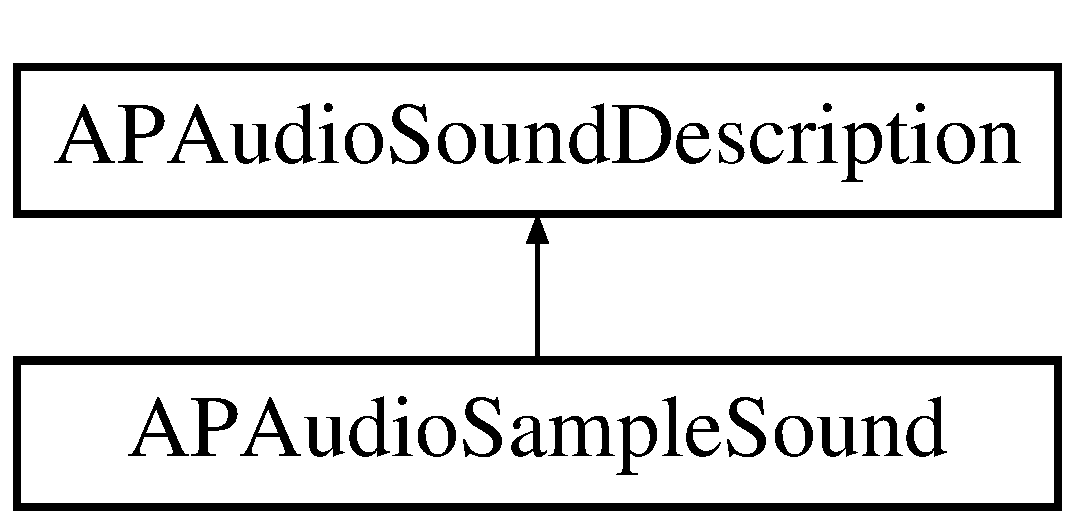
\includegraphics[height=2.000000cm]{class_a_p_audio_sound_description}
\end{center}
\end{figure}
\subsection*{Public Member Functions}
\begin{DoxyCompactItemize}
\item 
\hyperlink{class_a_p_audio_sound_description_a76cf64adbccf5889ed68d85d55ee84c2}{A\+P\+Audio\+Sound\+Description} ()
\item 
bool \hyperlink{class_a_p_audio_sound_description_ae70d06dfd589349677637944eb5c5749}{listens\+To\+Note} (int note)
\item 
bool \hyperlink{class_a_p_audio_sound_description_a3b885791067a1c7a395d8e4bf94cfba5}{listens\+To\+Channel} (int channel)
\item 
std\+::string \hyperlink{class_a_p_audio_sound_description_af619f3b304e36dbce36d40368daac12c}{get\+I\+D} ()
\item 
void \hyperlink{class_a_p_audio_sound_description_a4bb63a0cddd57b4351a8c81d29c9c425}{set\+Note\+To\+Listen\+To} (int note)
\item 
void \hyperlink{class_a_p_audio_sound_description_a410e761e9eeb1fb3ba8f4a8eb2435c48}{set\+Channel\+To\+Listen\+To} (int channel)
\item 
void \hyperlink{class_a_p_audio_sound_description_aecc9f38d3b4f0c459a7d230385afe281}{set\+I\+D} (std\+::string I\+D)
\item 
\hyperlink{class_a_p_audio_sound_description_a76cf64adbccf5889ed68d85d55ee84c2}{A\+P\+Audio\+Sound\+Description} ()
\item 
virtual \hyperlink{class_a_p_audio_sound_description_ab9e7c944d289ef31f6d71b246254bd95}{$\sim$\+A\+P\+Audio\+Sound\+Description} ()
\item 
virtual bool \hyperlink{class_a_p_audio_sound_description_af0e31cf64b1726fb97c9d027d2bc4c74}{listens\+To\+Note} (\hyperlink{_a_p_audio_module_8h_a9219378a2632ccf0389d00317ce8cdc4}{Control\+Value} note)=0
\item 
virtual bool \hyperlink{class_a_p_audio_sound_description_aa4ab161259b35de895c07eb718629b98}{listens\+To\+Channel} (\hyperlink{_a_p_audio_module_8h_a9219378a2632ccf0389d00317ce8cdc4}{Control\+Value} channel)=0
\item 
void \hyperlink{class_a_p_audio_sound_description_a3f6a4f1c923ef861586637429c87331d}{set\+I\+D} (String I\+D)
\item 
void \hyperlink{class_a_p_audio_sound_description_a07442fa084810f983751c383f7813c09}{set\+Range} (\hyperlink{_a_p_audio_module_8h_a9219378a2632ccf0389d00317ce8cdc4}{Control\+Value} min, \hyperlink{_a_p_audio_module_8h_a9219378a2632ccf0389d00317ce8cdc4}{Control\+Value} max)
\item 
void \hyperlink{class_a_p_audio_sound_description_a56d03478d380d97bdb15f0b11108b2ee}{set\+Length} (unsigned int length)
\item 
\hyperlink{_a_p_audio_module_8h_a9219378a2632ccf0389d00317ce8cdc4}{Control\+Value} \hyperlink{class_a_p_audio_sound_description_a3d3e50bef1d5036ba012da2b16e57010}{get\+Min\+Note} ()
\item 
\hyperlink{_a_p_audio_module_8h_a9219378a2632ccf0389d00317ce8cdc4}{Control\+Value} \hyperlink{class_a_p_audio_sound_description_a1c295a865cfb91ede4d872679e78802f}{get\+Max\+Note} ()
\item 
\hyperlink{_a_p_audio_module_8h_a9219378a2632ccf0389d00317ce8cdc4}{Control\+Value} \hyperlink{class_a_p_audio_sound_description_ad9c7933ebec95be118df2c6c50ea9082}{get\+Channel} ()
\end{DoxyCompactItemize}


\subsection{Constructor \& Destructor Documentation}
\hypertarget{class_a_p_audio_sound_description_a76cf64adbccf5889ed68d85d55ee84c2}{\index{A\+P\+Audio\+Sound\+Description@{A\+P\+Audio\+Sound\+Description}!A\+P\+Audio\+Sound\+Description@{A\+P\+Audio\+Sound\+Description}}
\index{A\+P\+Audio\+Sound\+Description@{A\+P\+Audio\+Sound\+Description}!A\+P\+Audio\+Sound\+Description@{A\+P\+Audio\+Sound\+Description}}
\subsubsection[{A\+P\+Audio\+Sound\+Description}]{\setlength{\rightskip}{0pt plus 5cm}A\+P\+Audio\+Sound\+Description\+::\+A\+P\+Audio\+Sound\+Description (
\begin{DoxyParamCaption}
{}
\end{DoxyParamCaption}
)}}\label{class_a_p_audio_sound_description_a76cf64adbccf5889ed68d85d55ee84c2}
\hypertarget{class_a_p_audio_sound_description_a76cf64adbccf5889ed68d85d55ee84c2}{\index{A\+P\+Audio\+Sound\+Description@{A\+P\+Audio\+Sound\+Description}!A\+P\+Audio\+Sound\+Description@{A\+P\+Audio\+Sound\+Description}}
\index{A\+P\+Audio\+Sound\+Description@{A\+P\+Audio\+Sound\+Description}!A\+P\+Audio\+Sound\+Description@{A\+P\+Audio\+Sound\+Description}}
\subsubsection[{A\+P\+Audio\+Sound\+Description}]{\setlength{\rightskip}{0pt plus 5cm}A\+P\+Audio\+Sound\+Description\+::\+A\+P\+Audio\+Sound\+Description (
\begin{DoxyParamCaption}
{}
\end{DoxyParamCaption}
)}}\label{class_a_p_audio_sound_description_a76cf64adbccf5889ed68d85d55ee84c2}
\hypertarget{class_a_p_audio_sound_description_ab9e7c944d289ef31f6d71b246254bd95}{\index{A\+P\+Audio\+Sound\+Description@{A\+P\+Audio\+Sound\+Description}!````~A\+P\+Audio\+Sound\+Description@{$\sim$\+A\+P\+Audio\+Sound\+Description}}
\index{````~A\+P\+Audio\+Sound\+Description@{$\sim$\+A\+P\+Audio\+Sound\+Description}!A\+P\+Audio\+Sound\+Description@{A\+P\+Audio\+Sound\+Description}}
\subsubsection[{$\sim$\+A\+P\+Audio\+Sound\+Description}]{\setlength{\rightskip}{0pt plus 5cm}A\+P\+Audio\+Sound\+Description\+::$\sim$\+A\+P\+Audio\+Sound\+Description (
\begin{DoxyParamCaption}
{}
\end{DoxyParamCaption}
)\hspace{0.3cm}{\ttfamily [virtual]}}}\label{class_a_p_audio_sound_description_ab9e7c944d289ef31f6d71b246254bd95}


\subsection{Member Function Documentation}
\hypertarget{class_a_p_audio_sound_description_ad9c7933ebec95be118df2c6c50ea9082}{\index{A\+P\+Audio\+Sound\+Description@{A\+P\+Audio\+Sound\+Description}!get\+Channel@{get\+Channel}}
\index{get\+Channel@{get\+Channel}!A\+P\+Audio\+Sound\+Description@{A\+P\+Audio\+Sound\+Description}}
\subsubsection[{get\+Channel}]{\setlength{\rightskip}{0pt plus 5cm}{\bf Control\+Value} A\+P\+Audio\+Sound\+Description\+::get\+Channel (
\begin{DoxyParamCaption}
{}
\end{DoxyParamCaption}
)\hspace{0.3cm}{\ttfamily [inline]}}}\label{class_a_p_audio_sound_description_ad9c7933ebec95be118df2c6c50ea9082}
\hypertarget{class_a_p_audio_sound_description_af619f3b304e36dbce36d40368daac12c}{\index{A\+P\+Audio\+Sound\+Description@{A\+P\+Audio\+Sound\+Description}!get\+I\+D@{get\+I\+D}}
\index{get\+I\+D@{get\+I\+D}!A\+P\+Audio\+Sound\+Description@{A\+P\+Audio\+Sound\+Description}}
\subsubsection[{get\+I\+D}]{\setlength{\rightskip}{0pt plus 5cm}std\+::string A\+P\+Audio\+Sound\+Description\+::get\+I\+D (
\begin{DoxyParamCaption}
{}
\end{DoxyParamCaption}
)}}\label{class_a_p_audio_sound_description_af619f3b304e36dbce36d40368daac12c}
\hypertarget{class_a_p_audio_sound_description_a1c295a865cfb91ede4d872679e78802f}{\index{A\+P\+Audio\+Sound\+Description@{A\+P\+Audio\+Sound\+Description}!get\+Max\+Note@{get\+Max\+Note}}
\index{get\+Max\+Note@{get\+Max\+Note}!A\+P\+Audio\+Sound\+Description@{A\+P\+Audio\+Sound\+Description}}
\subsubsection[{get\+Max\+Note}]{\setlength{\rightskip}{0pt plus 5cm}{\bf Control\+Value} A\+P\+Audio\+Sound\+Description\+::get\+Max\+Note (
\begin{DoxyParamCaption}
{}
\end{DoxyParamCaption}
)\hspace{0.3cm}{\ttfamily [inline]}}}\label{class_a_p_audio_sound_description_a1c295a865cfb91ede4d872679e78802f}
\hypertarget{class_a_p_audio_sound_description_a3d3e50bef1d5036ba012da2b16e57010}{\index{A\+P\+Audio\+Sound\+Description@{A\+P\+Audio\+Sound\+Description}!get\+Min\+Note@{get\+Min\+Note}}
\index{get\+Min\+Note@{get\+Min\+Note}!A\+P\+Audio\+Sound\+Description@{A\+P\+Audio\+Sound\+Description}}
\subsubsection[{get\+Min\+Note}]{\setlength{\rightskip}{0pt plus 5cm}{\bf Control\+Value} A\+P\+Audio\+Sound\+Description\+::get\+Min\+Note (
\begin{DoxyParamCaption}
{}
\end{DoxyParamCaption}
)\hspace{0.3cm}{\ttfamily [inline]}}}\label{class_a_p_audio_sound_description_a3d3e50bef1d5036ba012da2b16e57010}
\hypertarget{class_a_p_audio_sound_description_a3b885791067a1c7a395d8e4bf94cfba5}{\index{A\+P\+Audio\+Sound\+Description@{A\+P\+Audio\+Sound\+Description}!listens\+To\+Channel@{listens\+To\+Channel}}
\index{listens\+To\+Channel@{listens\+To\+Channel}!A\+P\+Audio\+Sound\+Description@{A\+P\+Audio\+Sound\+Description}}
\subsubsection[{listens\+To\+Channel}]{\setlength{\rightskip}{0pt plus 5cm}bool A\+P\+Audio\+Sound\+Description\+::listens\+To\+Channel (
\begin{DoxyParamCaption}
\item[{int}]{channel}
\end{DoxyParamCaption}
)}}\label{class_a_p_audio_sound_description_a3b885791067a1c7a395d8e4bf94cfba5}
\hypertarget{class_a_p_audio_sound_description_aa4ab161259b35de895c07eb718629b98}{\index{A\+P\+Audio\+Sound\+Description@{A\+P\+Audio\+Sound\+Description}!listens\+To\+Channel@{listens\+To\+Channel}}
\index{listens\+To\+Channel@{listens\+To\+Channel}!A\+P\+Audio\+Sound\+Description@{A\+P\+Audio\+Sound\+Description}}
\subsubsection[{listens\+To\+Channel}]{\setlength{\rightskip}{0pt plus 5cm}virtual bool A\+P\+Audio\+Sound\+Description\+::listens\+To\+Channel (
\begin{DoxyParamCaption}
\item[{{\bf Control\+Value}}]{channel}
\end{DoxyParamCaption}
)\hspace{0.3cm}{\ttfamily [pure virtual]}}}\label{class_a_p_audio_sound_description_aa4ab161259b35de895c07eb718629b98}


Implemented in \hyperlink{class_a_p_audio_sample_sound_a7498818340851d93745bc0d4946532f3}{A\+P\+Audio\+Sample\+Sound}.

\hypertarget{class_a_p_audio_sound_description_ae70d06dfd589349677637944eb5c5749}{\index{A\+P\+Audio\+Sound\+Description@{A\+P\+Audio\+Sound\+Description}!listens\+To\+Note@{listens\+To\+Note}}
\index{listens\+To\+Note@{listens\+To\+Note}!A\+P\+Audio\+Sound\+Description@{A\+P\+Audio\+Sound\+Description}}
\subsubsection[{listens\+To\+Note}]{\setlength{\rightskip}{0pt plus 5cm}bool A\+P\+Audio\+Sound\+Description\+::listens\+To\+Note (
\begin{DoxyParamCaption}
\item[{int}]{note}
\end{DoxyParamCaption}
)}}\label{class_a_p_audio_sound_description_ae70d06dfd589349677637944eb5c5749}
\hypertarget{class_a_p_audio_sound_description_af0e31cf64b1726fb97c9d027d2bc4c74}{\index{A\+P\+Audio\+Sound\+Description@{A\+P\+Audio\+Sound\+Description}!listens\+To\+Note@{listens\+To\+Note}}
\index{listens\+To\+Note@{listens\+To\+Note}!A\+P\+Audio\+Sound\+Description@{A\+P\+Audio\+Sound\+Description}}
\subsubsection[{listens\+To\+Note}]{\setlength{\rightskip}{0pt plus 5cm}virtual bool A\+P\+Audio\+Sound\+Description\+::listens\+To\+Note (
\begin{DoxyParamCaption}
\item[{{\bf Control\+Value}}]{note}
\end{DoxyParamCaption}
)\hspace{0.3cm}{\ttfamily [pure virtual]}}}\label{class_a_p_audio_sound_description_af0e31cf64b1726fb97c9d027d2bc4c74}


Implemented in \hyperlink{class_a_p_audio_sample_sound_a08d23ea13830a9251d638c77b5426e0d}{A\+P\+Audio\+Sample\+Sound}.

\hypertarget{class_a_p_audio_sound_description_a410e761e9eeb1fb3ba8f4a8eb2435c48}{\index{A\+P\+Audio\+Sound\+Description@{A\+P\+Audio\+Sound\+Description}!set\+Channel\+To\+Listen\+To@{set\+Channel\+To\+Listen\+To}}
\index{set\+Channel\+To\+Listen\+To@{set\+Channel\+To\+Listen\+To}!A\+P\+Audio\+Sound\+Description@{A\+P\+Audio\+Sound\+Description}}
\subsubsection[{set\+Channel\+To\+Listen\+To}]{\setlength{\rightskip}{0pt plus 5cm}void A\+P\+Audio\+Sound\+Description\+::set\+Channel\+To\+Listen\+To (
\begin{DoxyParamCaption}
\item[{int}]{channel}
\end{DoxyParamCaption}
)}}\label{class_a_p_audio_sound_description_a410e761e9eeb1fb3ba8f4a8eb2435c48}
\hypertarget{class_a_p_audio_sound_description_a3f6a4f1c923ef861586637429c87331d}{\index{A\+P\+Audio\+Sound\+Description@{A\+P\+Audio\+Sound\+Description}!set\+I\+D@{set\+I\+D}}
\index{set\+I\+D@{set\+I\+D}!A\+P\+Audio\+Sound\+Description@{A\+P\+Audio\+Sound\+Description}}
\subsubsection[{set\+I\+D}]{\setlength{\rightskip}{0pt plus 5cm}void A\+P\+Audio\+Sound\+Description\+::set\+I\+D (
\begin{DoxyParamCaption}
\item[{String}]{I\+D}
\end{DoxyParamCaption}
)}}\label{class_a_p_audio_sound_description_a3f6a4f1c923ef861586637429c87331d}
\hypertarget{class_a_p_audio_sound_description_aecc9f38d3b4f0c459a7d230385afe281}{\index{A\+P\+Audio\+Sound\+Description@{A\+P\+Audio\+Sound\+Description}!set\+I\+D@{set\+I\+D}}
\index{set\+I\+D@{set\+I\+D}!A\+P\+Audio\+Sound\+Description@{A\+P\+Audio\+Sound\+Description}}
\subsubsection[{set\+I\+D}]{\setlength{\rightskip}{0pt plus 5cm}void A\+P\+Audio\+Sound\+Description\+::set\+I\+D (
\begin{DoxyParamCaption}
\item[{std\+::string}]{I\+D}
\end{DoxyParamCaption}
)}}\label{class_a_p_audio_sound_description_aecc9f38d3b4f0c459a7d230385afe281}
\hypertarget{class_a_p_audio_sound_description_a56d03478d380d97bdb15f0b11108b2ee}{\index{A\+P\+Audio\+Sound\+Description@{A\+P\+Audio\+Sound\+Description}!set\+Length@{set\+Length}}
\index{set\+Length@{set\+Length}!A\+P\+Audio\+Sound\+Description@{A\+P\+Audio\+Sound\+Description}}
\subsubsection[{set\+Length}]{\setlength{\rightskip}{0pt plus 5cm}void A\+P\+Audio\+Sound\+Description\+::set\+Length (
\begin{DoxyParamCaption}
\item[{unsigned int}]{length}
\end{DoxyParamCaption}
)}}\label{class_a_p_audio_sound_description_a56d03478d380d97bdb15f0b11108b2ee}
\hypertarget{class_a_p_audio_sound_description_a4bb63a0cddd57b4351a8c81d29c9c425}{\index{A\+P\+Audio\+Sound\+Description@{A\+P\+Audio\+Sound\+Description}!set\+Note\+To\+Listen\+To@{set\+Note\+To\+Listen\+To}}
\index{set\+Note\+To\+Listen\+To@{set\+Note\+To\+Listen\+To}!A\+P\+Audio\+Sound\+Description@{A\+P\+Audio\+Sound\+Description}}
\subsubsection[{set\+Note\+To\+Listen\+To}]{\setlength{\rightskip}{0pt plus 5cm}void A\+P\+Audio\+Sound\+Description\+::set\+Note\+To\+Listen\+To (
\begin{DoxyParamCaption}
\item[{int}]{note}
\end{DoxyParamCaption}
)}}\label{class_a_p_audio_sound_description_a4bb63a0cddd57b4351a8c81d29c9c425}
\hypertarget{class_a_p_audio_sound_description_a07442fa084810f983751c383f7813c09}{\index{A\+P\+Audio\+Sound\+Description@{A\+P\+Audio\+Sound\+Description}!set\+Range@{set\+Range}}
\index{set\+Range@{set\+Range}!A\+P\+Audio\+Sound\+Description@{A\+P\+Audio\+Sound\+Description}}
\subsubsection[{set\+Range}]{\setlength{\rightskip}{0pt plus 5cm}void A\+P\+Audio\+Sound\+Description\+::set\+Range (
\begin{DoxyParamCaption}
\item[{{\bf Control\+Value}}]{min, }
\item[{{\bf Control\+Value}}]{max}
\end{DoxyParamCaption}
)}}\label{class_a_p_audio_sound_description_a07442fa084810f983751c383f7813c09}


The documentation for this class was generated from the following files\+:\begin{DoxyCompactItemize}
\item 
Audio Classes/\+Headers/\hyperlink{_audio_01_classes_2_headers_2_a_p_audio_sound_description_8h}{A\+P\+Audio\+Sound\+Description.\+h}\item 
Audio Classes/\+Implementations/\hyperlink{_audio_01_classes_2_implementations_2_a_p_audio_sound_description_8cpp}{A\+P\+Audio\+Sound\+Description.\+cpp}\end{DoxyCompactItemize}

\hypertarget{class_a_p_audio_source_manager}{\section{A\+P\+Audio\+Source\+Manager Class Reference}
\label{class_a_p_audio_source_manager}\index{A\+P\+Audio\+Source\+Manager@{A\+P\+Audio\+Source\+Manager}}
}


{\ttfamily \#include $<$A\+P\+Audio\+Source\+Manager.\+h$>$}

\subsection*{Public Member Functions}
\begin{DoxyCompactItemize}
\item 
\hyperlink{class_a_p_audio_source_manager_a5ebf363c61ac312788b03ed3d9b28ebd}{A\+P\+Audio\+Source\+Manager} ()
\item 
\hyperlink{class_a_p_audio_source_manager_aaebf9a9f1464c65a83b2536b9da195f7}{$\sim$\+A\+P\+Audio\+Source\+Manager} ()
\item 
\hyperlink{class_a_p_audio_sound_description}{A\+P\+Audio\+Sound\+Description} $\ast$ \hyperlink{class_a_p_audio_source_manager_a61a36d6d8f687d2774a896f0612d8d98}{load\+File} ()
\end{DoxyCompactItemize}


\subsection{Constructor \& Destructor Documentation}
\hypertarget{class_a_p_audio_source_manager_a5ebf363c61ac312788b03ed3d9b28ebd}{\index{A\+P\+Audio\+Source\+Manager@{A\+P\+Audio\+Source\+Manager}!A\+P\+Audio\+Source\+Manager@{A\+P\+Audio\+Source\+Manager}}
\index{A\+P\+Audio\+Source\+Manager@{A\+P\+Audio\+Source\+Manager}!A\+P\+Audio\+Source\+Manager@{A\+P\+Audio\+Source\+Manager}}
\subsubsection[{A\+P\+Audio\+Source\+Manager}]{\setlength{\rightskip}{0pt plus 5cm}A\+P\+Audio\+Source\+Manager\+::\+A\+P\+Audio\+Source\+Manager (
\begin{DoxyParamCaption}
{}
\end{DoxyParamCaption}
)}}\label{class_a_p_audio_source_manager_a5ebf363c61ac312788b03ed3d9b28ebd}
\hypertarget{class_a_p_audio_source_manager_aaebf9a9f1464c65a83b2536b9da195f7}{\index{A\+P\+Audio\+Source\+Manager@{A\+P\+Audio\+Source\+Manager}!````~A\+P\+Audio\+Source\+Manager@{$\sim$\+A\+P\+Audio\+Source\+Manager}}
\index{````~A\+P\+Audio\+Source\+Manager@{$\sim$\+A\+P\+Audio\+Source\+Manager}!A\+P\+Audio\+Source\+Manager@{A\+P\+Audio\+Source\+Manager}}
\subsubsection[{$\sim$\+A\+P\+Audio\+Source\+Manager}]{\setlength{\rightskip}{0pt plus 5cm}A\+P\+Audio\+Source\+Manager\+::$\sim$\+A\+P\+Audio\+Source\+Manager (
\begin{DoxyParamCaption}
{}
\end{DoxyParamCaption}
)}}\label{class_a_p_audio_source_manager_aaebf9a9f1464c65a83b2536b9da195f7}


\subsection{Member Function Documentation}
\hypertarget{class_a_p_audio_source_manager_a61a36d6d8f687d2774a896f0612d8d98}{\index{A\+P\+Audio\+Source\+Manager@{A\+P\+Audio\+Source\+Manager}!load\+File@{load\+File}}
\index{load\+File@{load\+File}!A\+P\+Audio\+Source\+Manager@{A\+P\+Audio\+Source\+Manager}}
\subsubsection[{load\+File}]{\setlength{\rightskip}{0pt plus 5cm}{\bf A\+P\+Audio\+Sound\+Description} $\ast$ A\+P\+Audio\+Source\+Manager\+::load\+File (
\begin{DoxyParamCaption}
{}
\end{DoxyParamCaption}
)}}\label{class_a_p_audio_source_manager_a61a36d6d8f687d2774a896f0612d8d98}


The documentation for this class was generated from the following files\+:\begin{DoxyCompactItemize}
\item 
In Development (don't include)/\hyperlink{_a_p_audio_source_manager_8h}{A\+P\+Audio\+Source\+Manager.\+h}\item 
In Development (don't include)/\hyperlink{_a_p_audio_source_manager_8cpp}{A\+P\+Audio\+Source\+Manager.\+cpp}\end{DoxyCompactItemize}

\hypertarget{class_a_p_audio_transport}{\section{A\+P\+Audio\+Transport Class Reference}
\label{class_a_p_audio_transport}\index{A\+P\+Audio\+Transport@{A\+P\+Audio\+Transport}}
}


{\ttfamily \#include $<$A\+P\+Audio\+Transport.\+h$>$}

\subsection*{Public Member Functions}
\begin{DoxyCompactItemize}
\item 
\hyperlink{class_a_p_audio_transport_aa1230745b38685c585ca1503e9fed59d}{A\+P\+Audio\+Transport} ()
\item 
void \hyperlink{class_a_p_audio_transport_a927b8d328f6eadab531b4b5a520f6d36}{update} (unsigned int time)
\item 
void \hyperlink{class_a_p_audio_transport_a0144ea9eb954e11bf7b1bdf948f2e0b8}{add\+Track} (\hyperlink{class_a_p_audio_sequencer}{A\+P\+Audio\+Sequencer} track)
\item 
void \hyperlink{class_a_p_audio_transport_acb41e3c57807cf1ab5db060e89ffb604}{play} ()
\item 
void \hyperlink{class_a_p_audio_transport_a5a0ea52ab96c056aea94e8924417ad08}{pause} ()
\item 
void \hyperlink{class_a_p_audio_transport_aa0647d0f7baabf9735c83d75308278f7}{stop} ()
\end{DoxyCompactItemize}


\subsection{Constructor \& Destructor Documentation}
\hypertarget{class_a_p_audio_transport_aa1230745b38685c585ca1503e9fed59d}{\index{A\+P\+Audio\+Transport@{A\+P\+Audio\+Transport}!A\+P\+Audio\+Transport@{A\+P\+Audio\+Transport}}
\index{A\+P\+Audio\+Transport@{A\+P\+Audio\+Transport}!A\+P\+Audio\+Transport@{A\+P\+Audio\+Transport}}
\subsubsection[{A\+P\+Audio\+Transport}]{\setlength{\rightskip}{0pt plus 5cm}A\+P\+Audio\+Transport\+::\+A\+P\+Audio\+Transport (
\begin{DoxyParamCaption}
{}
\end{DoxyParamCaption}
)}}\label{class_a_p_audio_transport_aa1230745b38685c585ca1503e9fed59d}


\subsection{Member Function Documentation}
\hypertarget{class_a_p_audio_transport_a0144ea9eb954e11bf7b1bdf948f2e0b8}{\index{A\+P\+Audio\+Transport@{A\+P\+Audio\+Transport}!add\+Track@{add\+Track}}
\index{add\+Track@{add\+Track}!A\+P\+Audio\+Transport@{A\+P\+Audio\+Transport}}
\subsubsection[{add\+Track}]{\setlength{\rightskip}{0pt plus 5cm}void A\+P\+Audio\+Transport\+::add\+Track (
\begin{DoxyParamCaption}
\item[{{\bf A\+P\+Audio\+Sequencer}}]{track}
\end{DoxyParamCaption}
)}}\label{class_a_p_audio_transport_a0144ea9eb954e11bf7b1bdf948f2e0b8}
\hypertarget{class_a_p_audio_transport_a5a0ea52ab96c056aea94e8924417ad08}{\index{A\+P\+Audio\+Transport@{A\+P\+Audio\+Transport}!pause@{pause}}
\index{pause@{pause}!A\+P\+Audio\+Transport@{A\+P\+Audio\+Transport}}
\subsubsection[{pause}]{\setlength{\rightskip}{0pt plus 5cm}void A\+P\+Audio\+Transport\+::pause (
\begin{DoxyParamCaption}
{}
\end{DoxyParamCaption}
)}}\label{class_a_p_audio_transport_a5a0ea52ab96c056aea94e8924417ad08}
\hypertarget{class_a_p_audio_transport_acb41e3c57807cf1ab5db060e89ffb604}{\index{A\+P\+Audio\+Transport@{A\+P\+Audio\+Transport}!play@{play}}
\index{play@{play}!A\+P\+Audio\+Transport@{A\+P\+Audio\+Transport}}
\subsubsection[{play}]{\setlength{\rightskip}{0pt plus 5cm}void A\+P\+Audio\+Transport\+::play (
\begin{DoxyParamCaption}
{}
\end{DoxyParamCaption}
)}}\label{class_a_p_audio_transport_acb41e3c57807cf1ab5db060e89ffb604}
\hypertarget{class_a_p_audio_transport_aa0647d0f7baabf9735c83d75308278f7}{\index{A\+P\+Audio\+Transport@{A\+P\+Audio\+Transport}!stop@{stop}}
\index{stop@{stop}!A\+P\+Audio\+Transport@{A\+P\+Audio\+Transport}}
\subsubsection[{stop}]{\setlength{\rightskip}{0pt plus 5cm}void A\+P\+Audio\+Transport\+::stop (
\begin{DoxyParamCaption}
{}
\end{DoxyParamCaption}
)}}\label{class_a_p_audio_transport_aa0647d0f7baabf9735c83d75308278f7}
\hypertarget{class_a_p_audio_transport_a927b8d328f6eadab531b4b5a520f6d36}{\index{A\+P\+Audio\+Transport@{A\+P\+Audio\+Transport}!update@{update}}
\index{update@{update}!A\+P\+Audio\+Transport@{A\+P\+Audio\+Transport}}
\subsubsection[{update}]{\setlength{\rightskip}{0pt plus 5cm}void A\+P\+Audio\+Transport\+::update (
\begin{DoxyParamCaption}
\item[{unsigned int}]{time}
\end{DoxyParamCaption}
)}}\label{class_a_p_audio_transport_a927b8d328f6eadab531b4b5a520f6d36}


The documentation for this class was generated from the following files\+:\begin{DoxyCompactItemize}
\item 
In Development (don't include)/\hyperlink{_a_p_audio_transport_8h}{A\+P\+Audio\+Transport.\+h}\item 
In Development (don't include)/\hyperlink{_a_p_audio_transport_8cpp}{A\+P\+Audio\+Transport.\+cpp}\end{DoxyCompactItemize}

\hypertarget{class_a_p_audio_voice}{\section{A\+P\+Audio\+Voice Class Reference}
\label{class_a_p_audio_voice}\index{A\+P\+Audio\+Voice@{A\+P\+Audio\+Voice}}
}


{\ttfamily \#include $<$A\+P\+Audio\+Voice.\+h$>$}

Inheritance diagram for A\+P\+Audio\+Voice\+:\begin{figure}[H]
\begin{center}
\leavevmode
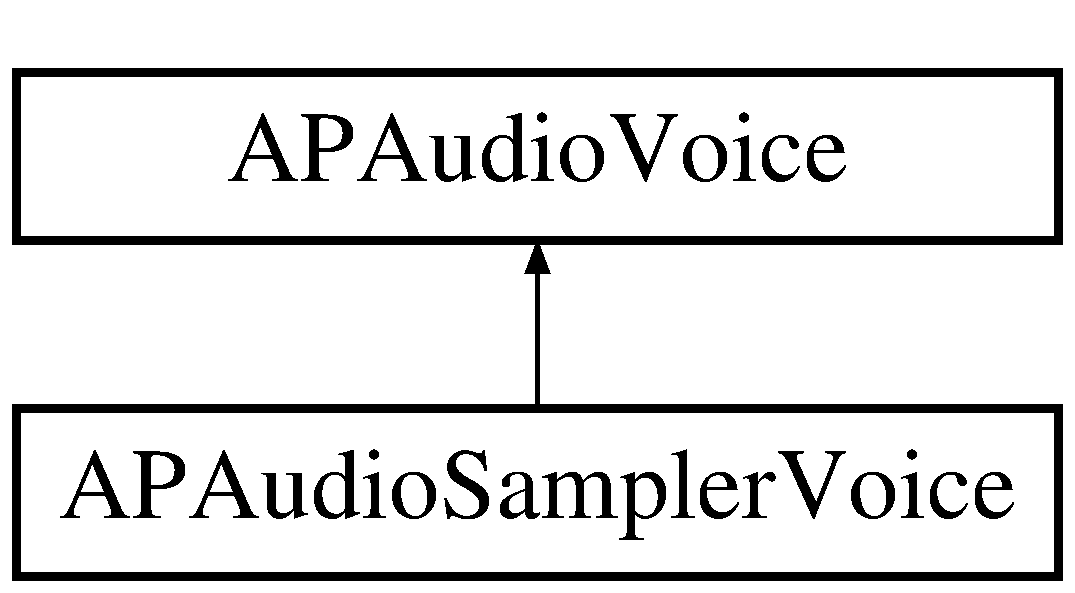
\includegraphics[height=2.000000cm]{class_a_p_audio_voice}
\end{center}
\end{figure}
\subsection*{Public Member Functions}
\begin{DoxyCompactItemize}
\item 
\hyperlink{class_a_p_audio_voice_a59098dc9b3c7b3f8cb369fef98c96506}{A\+P\+Audio\+Voice} ()
\item 
virtual \hyperlink{class_a_p_audio_voice_a7961e8c9c214303de643a6a30e232d47}{$\sim$\+A\+P\+Audio\+Voice} ()
\item 
virtual void \hyperlink{class_a_p_audio_voice_a151ae804092f9c6b9925f450565e3df4}{render\+Next\+Block} (\hyperlink{_a_p_audio_module_8h_a2c2f997fdc6b0e88b3723fb20dc502f0}{Sample\+Buffer} output\+Buffer, int start\+Sample, int num\+Samples, \hyperlink{_a_p_audio_module_8h_a9cc0620fb2e91b51587c6936060d4161}{U\+Int} channel)=0
\item 
virtual void \hyperlink{class_a_p_audio_voice_a25b0e54f49472f05ccafb38c782faae8}{stop\+Voice} ()=0
\item 
virtual bool \hyperlink{class_a_p_audio_voice_a4c534683ad441b5ff7e14ed528e058a4}{can\+Play\+Sound} (\hyperlink{class_a_p_audio_sound_description}{A\+P\+Audio\+Sound\+Description} $\ast$sound)=0
\item 
void \hyperlink{class_a_p_audio_voice_a5bf36c5ec20444b19e6f02c8a1a0ef7d}{set\+Sound} (\hyperlink{class_a_p_audio_sound_description}{A\+P\+Audio\+Sound\+Description} $\ast$sound)
\item 
void \hyperlink{class_a_p_audio_voice_ae14f422e9e88b3be33c2c75ac0876113}{release\+Voice} ()
\item 
void \hyperlink{class_a_p_audio_voice_aff7b4b5bbcc39b3f5f052ad9f5f1c883}{set\+Is\+Playing} (bool playing)
\item 
void \hyperlink{class_a_p_audio_voice_abec08aad18d389152591a381ae1932aa}{set\+Pitch} (\hyperlink{_a_p_audio_module_8h_a9219378a2632ccf0389d00317ce8cdc4}{Control\+Value} pitch)
\item 
void \hyperlink{class_a_p_audio_voice_ab77f46e9e96eed6a2ecf34d295c162b6}{set\+I\+D} (\hyperlink{_a_p_audio_module_8h_a9cc0620fb2e91b51587c6936060d4161}{U\+Int} I\+D)
\item 
\hyperlink{_a_p_audio_module_8h_a9cc0620fb2e91b51587c6936060d4161}{U\+Int} \hyperlink{class_a_p_audio_voice_a7a4588bb43f5c2618da0d0bd405296cc}{get\+I\+D} ()
\item 
bool \hyperlink{class_a_p_audio_voice_ade02900fae46f947b66bfb5148cd282d}{get\+Is\+Playing} ()
\item 
\hyperlink{_a_p_audio_module_8h_a9219378a2632ccf0389d00317ce8cdc4}{Control\+Value} \hyperlink{class_a_p_audio_voice_a505816cfb3fddbbf8fe23a8391142f5c}{get\+Pitch} ()
\item 
\hyperlink{class_a_p_audio_sound_description}{A\+P\+Audio\+Sound\+Description} $\ast$ \hyperlink{class_a_p_audio_voice_a6e4872c0f74fee2796bf402e51fc28a3}{get\+Sound} ()
\item 
\hyperlink{class_a_p_audio_envelope}{A\+P\+Audio\+Envelope} $\ast$ \hyperlink{class_a_p_audio_voice_a8b28ea28b7372dd8cc17039c303dbdd3}{get\+Envelope} () const 
\item 
virtual void \hyperlink{class_a_p_audio_voice_a9d8807cb399e9d5fb5ce207ab9f89416}{reset} ()=0
\end{DoxyCompactItemize}
\subsection*{Friends}
\begin{DoxyCompactItemize}
\item 
class \hyperlink{class_a_p_audio_voice_ab3756667a3eeab1aa8d1398d2cfce2eb}{A\+P\+Audio\+Voice\+Manager}
\end{DoxyCompactItemize}


\subsection{Constructor \& Destructor Documentation}
\hypertarget{class_a_p_audio_voice_a59098dc9b3c7b3f8cb369fef98c96506}{\index{A\+P\+Audio\+Voice@{A\+P\+Audio\+Voice}!A\+P\+Audio\+Voice@{A\+P\+Audio\+Voice}}
\index{A\+P\+Audio\+Voice@{A\+P\+Audio\+Voice}!A\+P\+Audio\+Voice@{A\+P\+Audio\+Voice}}
\subsubsection[{A\+P\+Audio\+Voice}]{\setlength{\rightskip}{0pt plus 5cm}A\+P\+Audio\+Voice\+::\+A\+P\+Audio\+Voice (
\begin{DoxyParamCaption}
{}
\end{DoxyParamCaption}
)}}\label{class_a_p_audio_voice_a59098dc9b3c7b3f8cb369fef98c96506}
\hypertarget{class_a_p_audio_voice_a7961e8c9c214303de643a6a30e232d47}{\index{A\+P\+Audio\+Voice@{A\+P\+Audio\+Voice}!````~A\+P\+Audio\+Voice@{$\sim$\+A\+P\+Audio\+Voice}}
\index{````~A\+P\+Audio\+Voice@{$\sim$\+A\+P\+Audio\+Voice}!A\+P\+Audio\+Voice@{A\+P\+Audio\+Voice}}
\subsubsection[{$\sim$\+A\+P\+Audio\+Voice}]{\setlength{\rightskip}{0pt plus 5cm}A\+P\+Audio\+Voice\+::$\sim$\+A\+P\+Audio\+Voice (
\begin{DoxyParamCaption}
{}
\end{DoxyParamCaption}
)\hspace{0.3cm}{\ttfamily [virtual]}}}\label{class_a_p_audio_voice_a7961e8c9c214303de643a6a30e232d47}


\subsection{Member Function Documentation}
\hypertarget{class_a_p_audio_voice_a4c534683ad441b5ff7e14ed528e058a4}{\index{A\+P\+Audio\+Voice@{A\+P\+Audio\+Voice}!can\+Play\+Sound@{can\+Play\+Sound}}
\index{can\+Play\+Sound@{can\+Play\+Sound}!A\+P\+Audio\+Voice@{A\+P\+Audio\+Voice}}
\subsubsection[{can\+Play\+Sound}]{\setlength{\rightskip}{0pt plus 5cm}virtual bool A\+P\+Audio\+Voice\+::can\+Play\+Sound (
\begin{DoxyParamCaption}
\item[{{\bf A\+P\+Audio\+Sound\+Description} $\ast$}]{sound}
\end{DoxyParamCaption}
)\hspace{0.3cm}{\ttfamily [pure virtual]}}}\label{class_a_p_audio_voice_a4c534683ad441b5ff7e14ed528e058a4}


Implemented in \hyperlink{class_a_p_audio_sampler_voice_af9959b4be2689341d32e697b5cef7ab5}{A\+P\+Audio\+Sampler\+Voice}.

\hypertarget{class_a_p_audio_voice_a8b28ea28b7372dd8cc17039c303dbdd3}{\index{A\+P\+Audio\+Voice@{A\+P\+Audio\+Voice}!get\+Envelope@{get\+Envelope}}
\index{get\+Envelope@{get\+Envelope}!A\+P\+Audio\+Voice@{A\+P\+Audio\+Voice}}
\subsubsection[{get\+Envelope}]{\setlength{\rightskip}{0pt plus 5cm}{\bf A\+P\+Audio\+Envelope}$\ast$ A\+P\+Audio\+Voice\+::get\+Envelope (
\begin{DoxyParamCaption}
{}
\end{DoxyParamCaption}
) const\hspace{0.3cm}{\ttfamily [inline]}}}\label{class_a_p_audio_voice_a8b28ea28b7372dd8cc17039c303dbdd3}
\hypertarget{class_a_p_audio_voice_a7a4588bb43f5c2618da0d0bd405296cc}{\index{A\+P\+Audio\+Voice@{A\+P\+Audio\+Voice}!get\+I\+D@{get\+I\+D}}
\index{get\+I\+D@{get\+I\+D}!A\+P\+Audio\+Voice@{A\+P\+Audio\+Voice}}
\subsubsection[{get\+I\+D}]{\setlength{\rightskip}{0pt plus 5cm}{\bf U\+Int} A\+P\+Audio\+Voice\+::get\+I\+D (
\begin{DoxyParamCaption}
{}
\end{DoxyParamCaption}
)\hspace{0.3cm}{\ttfamily [inline]}}}\label{class_a_p_audio_voice_a7a4588bb43f5c2618da0d0bd405296cc}
\hypertarget{class_a_p_audio_voice_ade02900fae46f947b66bfb5148cd282d}{\index{A\+P\+Audio\+Voice@{A\+P\+Audio\+Voice}!get\+Is\+Playing@{get\+Is\+Playing}}
\index{get\+Is\+Playing@{get\+Is\+Playing}!A\+P\+Audio\+Voice@{A\+P\+Audio\+Voice}}
\subsubsection[{get\+Is\+Playing}]{\setlength{\rightskip}{0pt plus 5cm}bool A\+P\+Audio\+Voice\+::get\+Is\+Playing (
\begin{DoxyParamCaption}
{}
\end{DoxyParamCaption}
)\hspace{0.3cm}{\ttfamily [inline]}}}\label{class_a_p_audio_voice_ade02900fae46f947b66bfb5148cd282d}
\hypertarget{class_a_p_audio_voice_a505816cfb3fddbbf8fe23a8391142f5c}{\index{A\+P\+Audio\+Voice@{A\+P\+Audio\+Voice}!get\+Pitch@{get\+Pitch}}
\index{get\+Pitch@{get\+Pitch}!A\+P\+Audio\+Voice@{A\+P\+Audio\+Voice}}
\subsubsection[{get\+Pitch}]{\setlength{\rightskip}{0pt plus 5cm}{\bf Control\+Value} A\+P\+Audio\+Voice\+::get\+Pitch (
\begin{DoxyParamCaption}
{}
\end{DoxyParamCaption}
)\hspace{0.3cm}{\ttfamily [inline]}}}\label{class_a_p_audio_voice_a505816cfb3fddbbf8fe23a8391142f5c}
\hypertarget{class_a_p_audio_voice_a6e4872c0f74fee2796bf402e51fc28a3}{\index{A\+P\+Audio\+Voice@{A\+P\+Audio\+Voice}!get\+Sound@{get\+Sound}}
\index{get\+Sound@{get\+Sound}!A\+P\+Audio\+Voice@{A\+P\+Audio\+Voice}}
\subsubsection[{get\+Sound}]{\setlength{\rightskip}{0pt plus 5cm}{\bf A\+P\+Audio\+Sound\+Description}$\ast$ A\+P\+Audio\+Voice\+::get\+Sound (
\begin{DoxyParamCaption}
{}
\end{DoxyParamCaption}
)\hspace{0.3cm}{\ttfamily [inline]}}}\label{class_a_p_audio_voice_a6e4872c0f74fee2796bf402e51fc28a3}
\hypertarget{class_a_p_audio_voice_ae14f422e9e88b3be33c2c75ac0876113}{\index{A\+P\+Audio\+Voice@{A\+P\+Audio\+Voice}!release\+Voice@{release\+Voice}}
\index{release\+Voice@{release\+Voice}!A\+P\+Audio\+Voice@{A\+P\+Audio\+Voice}}
\subsubsection[{release\+Voice}]{\setlength{\rightskip}{0pt plus 5cm}void A\+P\+Audio\+Voice\+::release\+Voice (
\begin{DoxyParamCaption}
{}
\end{DoxyParamCaption}
)}}\label{class_a_p_audio_voice_ae14f422e9e88b3be33c2c75ac0876113}
\hypertarget{class_a_p_audio_voice_a151ae804092f9c6b9925f450565e3df4}{\index{A\+P\+Audio\+Voice@{A\+P\+Audio\+Voice}!render\+Next\+Block@{render\+Next\+Block}}
\index{render\+Next\+Block@{render\+Next\+Block}!A\+P\+Audio\+Voice@{A\+P\+Audio\+Voice}}
\subsubsection[{render\+Next\+Block}]{\setlength{\rightskip}{0pt plus 5cm}virtual void A\+P\+Audio\+Voice\+::render\+Next\+Block (
\begin{DoxyParamCaption}
\item[{{\bf Sample\+Buffer}}]{output\+Buffer, }
\item[{int}]{start\+Sample, }
\item[{int}]{num\+Samples, }
\item[{{\bf U\+Int}}]{channel}
\end{DoxyParamCaption}
)\hspace{0.3cm}{\ttfamily [pure virtual]}}}\label{class_a_p_audio_voice_a151ae804092f9c6b9925f450565e3df4}


Implemented in \hyperlink{class_a_p_audio_sampler_voice_a2771cb306e331a458cea4283048c374c}{A\+P\+Audio\+Sampler\+Voice}.

\hypertarget{class_a_p_audio_voice_a9d8807cb399e9d5fb5ce207ab9f89416}{\index{A\+P\+Audio\+Voice@{A\+P\+Audio\+Voice}!reset@{reset}}
\index{reset@{reset}!A\+P\+Audio\+Voice@{A\+P\+Audio\+Voice}}
\subsubsection[{reset}]{\setlength{\rightskip}{0pt plus 5cm}virtual void A\+P\+Audio\+Voice\+::reset (
\begin{DoxyParamCaption}
{}
\end{DoxyParamCaption}
)\hspace{0.3cm}{\ttfamily [pure virtual]}}}\label{class_a_p_audio_voice_a9d8807cb399e9d5fb5ce207ab9f89416}


Implemented in \hyperlink{class_a_p_audio_sampler_voice_acc47dbbd5d5835092c4806d245c53188}{A\+P\+Audio\+Sampler\+Voice}.

\hypertarget{class_a_p_audio_voice_ab77f46e9e96eed6a2ecf34d295c162b6}{\index{A\+P\+Audio\+Voice@{A\+P\+Audio\+Voice}!set\+I\+D@{set\+I\+D}}
\index{set\+I\+D@{set\+I\+D}!A\+P\+Audio\+Voice@{A\+P\+Audio\+Voice}}
\subsubsection[{set\+I\+D}]{\setlength{\rightskip}{0pt plus 5cm}void A\+P\+Audio\+Voice\+::set\+I\+D (
\begin{DoxyParamCaption}
\item[{{\bf U\+Int}}]{I\+D}
\end{DoxyParamCaption}
)}}\label{class_a_p_audio_voice_ab77f46e9e96eed6a2ecf34d295c162b6}
\hypertarget{class_a_p_audio_voice_aff7b4b5bbcc39b3f5f052ad9f5f1c883}{\index{A\+P\+Audio\+Voice@{A\+P\+Audio\+Voice}!set\+Is\+Playing@{set\+Is\+Playing}}
\index{set\+Is\+Playing@{set\+Is\+Playing}!A\+P\+Audio\+Voice@{A\+P\+Audio\+Voice}}
\subsubsection[{set\+Is\+Playing}]{\setlength{\rightskip}{0pt plus 5cm}void A\+P\+Audio\+Voice\+::set\+Is\+Playing (
\begin{DoxyParamCaption}
\item[{bool}]{playing}
\end{DoxyParamCaption}
)}}\label{class_a_p_audio_voice_aff7b4b5bbcc39b3f5f052ad9f5f1c883}
\hypertarget{class_a_p_audio_voice_abec08aad18d389152591a381ae1932aa}{\index{A\+P\+Audio\+Voice@{A\+P\+Audio\+Voice}!set\+Pitch@{set\+Pitch}}
\index{set\+Pitch@{set\+Pitch}!A\+P\+Audio\+Voice@{A\+P\+Audio\+Voice}}
\subsubsection[{set\+Pitch}]{\setlength{\rightskip}{0pt plus 5cm}void A\+P\+Audio\+Voice\+::set\+Pitch (
\begin{DoxyParamCaption}
\item[{{\bf Control\+Value}}]{pitch}
\end{DoxyParamCaption}
)}}\label{class_a_p_audio_voice_abec08aad18d389152591a381ae1932aa}
\hypertarget{class_a_p_audio_voice_a5bf36c5ec20444b19e6f02c8a1a0ef7d}{\index{A\+P\+Audio\+Voice@{A\+P\+Audio\+Voice}!set\+Sound@{set\+Sound}}
\index{set\+Sound@{set\+Sound}!A\+P\+Audio\+Voice@{A\+P\+Audio\+Voice}}
\subsubsection[{set\+Sound}]{\setlength{\rightskip}{0pt plus 5cm}void A\+P\+Audio\+Voice\+::set\+Sound (
\begin{DoxyParamCaption}
\item[{{\bf A\+P\+Audio\+Sound\+Description} $\ast$}]{sound}
\end{DoxyParamCaption}
)}}\label{class_a_p_audio_voice_a5bf36c5ec20444b19e6f02c8a1a0ef7d}
\hypertarget{class_a_p_audio_voice_a25b0e54f49472f05ccafb38c782faae8}{\index{A\+P\+Audio\+Voice@{A\+P\+Audio\+Voice}!stop\+Voice@{stop\+Voice}}
\index{stop\+Voice@{stop\+Voice}!A\+P\+Audio\+Voice@{A\+P\+Audio\+Voice}}
\subsubsection[{stop\+Voice}]{\setlength{\rightskip}{0pt plus 5cm}virtual void A\+P\+Audio\+Voice\+::stop\+Voice (
\begin{DoxyParamCaption}
{}
\end{DoxyParamCaption}
)\hspace{0.3cm}{\ttfamily [pure virtual]}}}\label{class_a_p_audio_voice_a25b0e54f49472f05ccafb38c782faae8}


Implemented in \hyperlink{class_a_p_audio_sampler_voice_af251bd2529b4472729db61d54753cc56}{A\+P\+Audio\+Sampler\+Voice}.



\subsection{Friends And Related Function Documentation}
\hypertarget{class_a_p_audio_voice_ab3756667a3eeab1aa8d1398d2cfce2eb}{\index{A\+P\+Audio\+Voice@{A\+P\+Audio\+Voice}!A\+P\+Audio\+Voice\+Manager@{A\+P\+Audio\+Voice\+Manager}}
\index{A\+P\+Audio\+Voice\+Manager@{A\+P\+Audio\+Voice\+Manager}!A\+P\+Audio\+Voice@{A\+P\+Audio\+Voice}}
\subsubsection[{A\+P\+Audio\+Voice\+Manager}]{\setlength{\rightskip}{0pt plus 5cm}friend class {\bf A\+P\+Audio\+Voice\+Manager}\hspace{0.3cm}{\ttfamily [friend]}}}\label{class_a_p_audio_voice_ab3756667a3eeab1aa8d1398d2cfce2eb}


The documentation for this class was generated from the following files\+:\begin{DoxyCompactItemize}
\item 
In Development (don't include)/\hyperlink{_a_p_audio_voice_8h}{A\+P\+Audio\+Voice.\+h}\item 
In Development (don't include)/\hyperlink{_a_p_audio_voice_8cpp}{A\+P\+Audio\+Voice.\+cpp}\end{DoxyCompactItemize}

\hypertarget{class_a_p_audio_voice_manager}{\section{A\+P\+Audio\+Voice\+Manager Class Reference}
\label{class_a_p_audio_voice_manager}\index{A\+P\+Audio\+Voice\+Manager@{A\+P\+Audio\+Voice\+Manager}}
}


{\ttfamily \#include $<$A\+P\+Audio\+Voice\+Manager.\+h$>$}

Inheritance diagram for A\+P\+Audio\+Voice\+Manager\+:\begin{figure}[H]
\begin{center}
\leavevmode
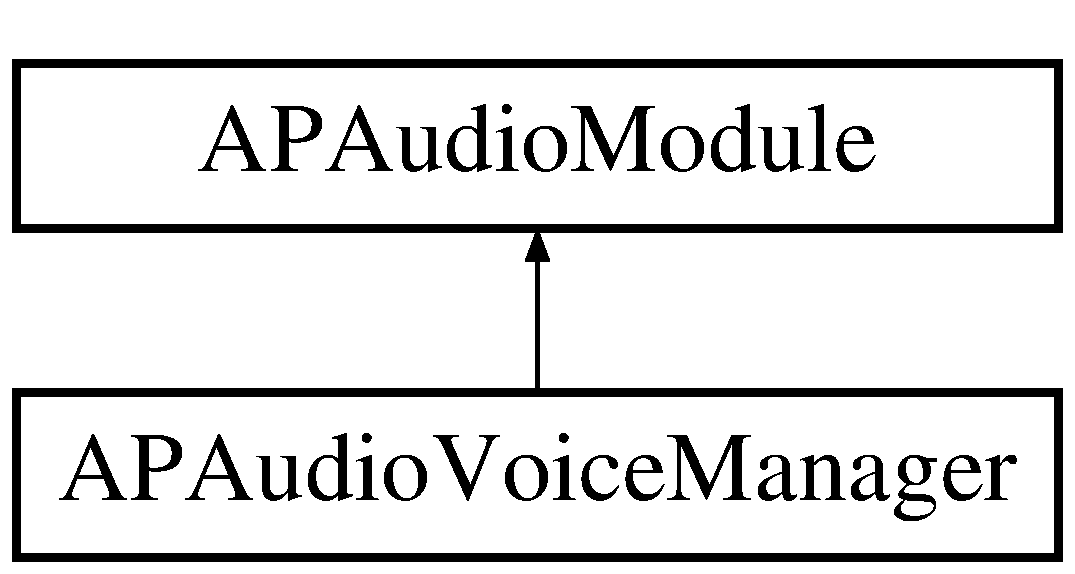
\includegraphics[height=2.000000cm]{class_a_p_audio_voice_manager}
\end{center}
\end{figure}
\subsection*{Public Member Functions}
\begin{DoxyCompactItemize}
\item 
\hyperlink{class_a_p_audio_voice_manager_ae34297343b744525fea2d52a0453b94a}{A\+P\+Audio\+Voice\+Manager} (\hyperlink{class_a_p_audio_main_frame}{A\+P\+Audio\+Main\+Frame} $\ast$mf, \hyperlink{_a_p_audio_module_8h_a9cc0620fb2e91b51587c6936060d4161}{U\+Int} channel)
\item 
\hyperlink{class_a_p_audio_voice}{A\+P\+Audio\+Voice} $\ast$ \hyperlink{class_a_p_audio_voice_manager_a481b2d864153250f25ef94721937b1b4}{find\+Free\+Voice} (\hyperlink{class_a_p_audio_sound_description}{A\+P\+Audio\+Sound\+Description} $\ast$sound\+Description, \hyperlink{_a_p_audio_module_8h_a9219378a2632ccf0389d00317ce8cdc4}{Control\+Value} pitch)
\item 
void \hyperlink{class_a_p_audio_voice_manager_a6ba625401b9c6c3ce347e5fb66c88a0b}{note\+On} (\hyperlink{_a_p_audio_module_8h_a9219378a2632ccf0389d00317ce8cdc4}{Control\+Value} pitch, \hyperlink{_a_p_audio_module_8h_a9219378a2632ccf0389d00317ce8cdc4}{Control\+Value} I\+D)
\item 
void \hyperlink{class_a_p_audio_voice_manager_a38206c6acb123bb6687103de073e2cdf}{note\+Off} (\hyperlink{_a_p_audio_module_8h_a9cc0620fb2e91b51587c6936060d4161}{U\+Int} I\+D)
\item 
void \hyperlink{class_a_p_audio_voice_manager_a54341a861884214078d658253cc104b7}{update\+Pitch} (\hyperlink{_a_p_audio_module_8h_a9219378a2632ccf0389d00317ce8cdc4}{Control\+Value} pitch, \hyperlink{_a_p_audio_module_8h_a9219378a2632ccf0389d00317ce8cdc4}{Control\+Value} I\+D)
\item 
void \hyperlink{class_a_p_audio_voice_manager_a3c2c148baa9205a99abc3036d801694e}{add\+Sound} (\hyperlink{class_a_p_audio_sound_description}{A\+P\+Audio\+Sound\+Description} $\ast$s)
\item 
void \hyperlink{class_a_p_audio_voice_manager_ac06498da7a38c87d4cc72fd44ce4b2ef}{start\+Voice} (\hyperlink{class_a_p_audio_voice}{A\+P\+Audio\+Voice} $\ast$voice, \hyperlink{class_a_p_audio_sound_description}{A\+P\+Audio\+Sound\+Description} $\ast$sound, \hyperlink{_a_p_audio_module_8h_a9219378a2632ccf0389d00317ce8cdc4}{Control\+Value} pitch, \hyperlink{_a_p_audio_module_8h_a9219378a2632ccf0389d00317ce8cdc4}{Control\+Value} velocity)
\item 
void \hyperlink{class_a_p_audio_voice_manager_aa57022af78e9b348b20159e27ae15320}{add\+Sampler\+Voice} ()
\item 
void \hyperlink{class_a_p_audio_voice_manager_a199d3d41d181ac4fc983f25ae5a30b94}{destroy\+All\+Voices} ()
\item 
void \hyperlink{class_a_p_audio_voice_manager_a27033002e3ab86c55ec5d1e5150d1892}{calculate\+Buffer} () override
\item 
\hyperlink{_a_p_audio_module_8h_a9cc0620fb2e91b51587c6936060d4161}{U\+Int} \hyperlink{class_a_p_audio_voice_manager_a9cbeb96228989601bede52821b8c829a}{get\+Active\+Voices} ()
\end{DoxyCompactItemize}
\subsection*{Public Attributes}
\begin{DoxyCompactItemize}
\item 
std\+::vector$<$ \hyperlink{class_a_p_audio_voice}{A\+P\+Audio\+Voice} $\ast$ $>$ \hyperlink{class_a_p_audio_voice_manager_a475d91a65b916d5247db02a1862b13f8}{voices}
\item 
std\+::vector\\*
$<$ \hyperlink{class_a_p_audio_sound_description}{A\+P\+Audio\+Sound\+Description} $\ast$ $>$ \hyperlink{class_a_p_audio_voice_manager_a8f0573dd9da39ac48fef87e31315939e}{sounds}
\end{DoxyCompactItemize}


\subsection{Constructor \& Destructor Documentation}
\hypertarget{class_a_p_audio_voice_manager_ae34297343b744525fea2d52a0453b94a}{\index{A\+P\+Audio\+Voice\+Manager@{A\+P\+Audio\+Voice\+Manager}!A\+P\+Audio\+Voice\+Manager@{A\+P\+Audio\+Voice\+Manager}}
\index{A\+P\+Audio\+Voice\+Manager@{A\+P\+Audio\+Voice\+Manager}!A\+P\+Audio\+Voice\+Manager@{A\+P\+Audio\+Voice\+Manager}}
\subsubsection[{A\+P\+Audio\+Voice\+Manager}]{\setlength{\rightskip}{0pt plus 5cm}A\+P\+Audio\+Voice\+Manager\+::\+A\+P\+Audio\+Voice\+Manager (
\begin{DoxyParamCaption}
\item[{{\bf A\+P\+Audio\+Main\+Frame} $\ast$}]{mf, }
\item[{{\bf U\+Int}}]{channel}
\end{DoxyParamCaption}
)}}\label{class_a_p_audio_voice_manager_ae34297343b744525fea2d52a0453b94a}


\subsection{Member Function Documentation}
\hypertarget{class_a_p_audio_voice_manager_aa57022af78e9b348b20159e27ae15320}{\index{A\+P\+Audio\+Voice\+Manager@{A\+P\+Audio\+Voice\+Manager}!add\+Sampler\+Voice@{add\+Sampler\+Voice}}
\index{add\+Sampler\+Voice@{add\+Sampler\+Voice}!A\+P\+Audio\+Voice\+Manager@{A\+P\+Audio\+Voice\+Manager}}
\subsubsection[{add\+Sampler\+Voice}]{\setlength{\rightskip}{0pt plus 5cm}void A\+P\+Audio\+Voice\+Manager\+::add\+Sampler\+Voice (
\begin{DoxyParamCaption}
{}
\end{DoxyParamCaption}
)}}\label{class_a_p_audio_voice_manager_aa57022af78e9b348b20159e27ae15320}
\hypertarget{class_a_p_audio_voice_manager_a3c2c148baa9205a99abc3036d801694e}{\index{A\+P\+Audio\+Voice\+Manager@{A\+P\+Audio\+Voice\+Manager}!add\+Sound@{add\+Sound}}
\index{add\+Sound@{add\+Sound}!A\+P\+Audio\+Voice\+Manager@{A\+P\+Audio\+Voice\+Manager}}
\subsubsection[{add\+Sound}]{\setlength{\rightskip}{0pt plus 5cm}void A\+P\+Audio\+Voice\+Manager\+::add\+Sound (
\begin{DoxyParamCaption}
\item[{{\bf A\+P\+Audio\+Sound\+Description} $\ast$}]{s}
\end{DoxyParamCaption}
)}}\label{class_a_p_audio_voice_manager_a3c2c148baa9205a99abc3036d801694e}
\hypertarget{class_a_p_audio_voice_manager_a27033002e3ab86c55ec5d1e5150d1892}{\index{A\+P\+Audio\+Voice\+Manager@{A\+P\+Audio\+Voice\+Manager}!calculate\+Buffer@{calculate\+Buffer}}
\index{calculate\+Buffer@{calculate\+Buffer}!A\+P\+Audio\+Voice\+Manager@{A\+P\+Audio\+Voice\+Manager}}
\subsubsection[{calculate\+Buffer}]{\setlength{\rightskip}{0pt plus 5cm}void A\+P\+Audio\+Voice\+Manager\+::calculate\+Buffer (
\begin{DoxyParamCaption}
{}
\end{DoxyParamCaption}
)\hspace{0.3cm}{\ttfamily [override]}, {\ttfamily [virtual]}}}\label{class_a_p_audio_voice_manager_a27033002e3ab86c55ec5d1e5150d1892}


Reimplemented from \hyperlink{class_a_p_audio_module_a10c6d7f469b9d1626a80c4d745663a2a}{A\+P\+Audio\+Module}.

\hypertarget{class_a_p_audio_voice_manager_a199d3d41d181ac4fc983f25ae5a30b94}{\index{A\+P\+Audio\+Voice\+Manager@{A\+P\+Audio\+Voice\+Manager}!destroy\+All\+Voices@{destroy\+All\+Voices}}
\index{destroy\+All\+Voices@{destroy\+All\+Voices}!A\+P\+Audio\+Voice\+Manager@{A\+P\+Audio\+Voice\+Manager}}
\subsubsection[{destroy\+All\+Voices}]{\setlength{\rightskip}{0pt plus 5cm}void A\+P\+Audio\+Voice\+Manager\+::destroy\+All\+Voices (
\begin{DoxyParamCaption}
{}
\end{DoxyParamCaption}
)}}\label{class_a_p_audio_voice_manager_a199d3d41d181ac4fc983f25ae5a30b94}
\hypertarget{class_a_p_audio_voice_manager_a481b2d864153250f25ef94721937b1b4}{\index{A\+P\+Audio\+Voice\+Manager@{A\+P\+Audio\+Voice\+Manager}!find\+Free\+Voice@{find\+Free\+Voice}}
\index{find\+Free\+Voice@{find\+Free\+Voice}!A\+P\+Audio\+Voice\+Manager@{A\+P\+Audio\+Voice\+Manager}}
\subsubsection[{find\+Free\+Voice}]{\setlength{\rightskip}{0pt plus 5cm}{\bf A\+P\+Audio\+Voice} $\ast$ A\+P\+Audio\+Voice\+Manager\+::find\+Free\+Voice (
\begin{DoxyParamCaption}
\item[{{\bf A\+P\+Audio\+Sound\+Description} $\ast$}]{sound\+Description, }
\item[{{\bf Control\+Value}}]{pitch}
\end{DoxyParamCaption}
)}}\label{class_a_p_audio_voice_manager_a481b2d864153250f25ef94721937b1b4}
\hypertarget{class_a_p_audio_voice_manager_a9cbeb96228989601bede52821b8c829a}{\index{A\+P\+Audio\+Voice\+Manager@{A\+P\+Audio\+Voice\+Manager}!get\+Active\+Voices@{get\+Active\+Voices}}
\index{get\+Active\+Voices@{get\+Active\+Voices}!A\+P\+Audio\+Voice\+Manager@{A\+P\+Audio\+Voice\+Manager}}
\subsubsection[{get\+Active\+Voices}]{\setlength{\rightskip}{0pt plus 5cm}{\bf U\+Int} A\+P\+Audio\+Voice\+Manager\+::get\+Active\+Voices (
\begin{DoxyParamCaption}
{}
\end{DoxyParamCaption}
)}}\label{class_a_p_audio_voice_manager_a9cbeb96228989601bede52821b8c829a}
\hypertarget{class_a_p_audio_voice_manager_a38206c6acb123bb6687103de073e2cdf}{\index{A\+P\+Audio\+Voice\+Manager@{A\+P\+Audio\+Voice\+Manager}!note\+Off@{note\+Off}}
\index{note\+Off@{note\+Off}!A\+P\+Audio\+Voice\+Manager@{A\+P\+Audio\+Voice\+Manager}}
\subsubsection[{note\+Off}]{\setlength{\rightskip}{0pt plus 5cm}void A\+P\+Audio\+Voice\+Manager\+::note\+Off (
\begin{DoxyParamCaption}
\item[{{\bf U\+Int}}]{I\+D}
\end{DoxyParamCaption}
)}}\label{class_a_p_audio_voice_manager_a38206c6acb123bb6687103de073e2cdf}
\hypertarget{class_a_p_audio_voice_manager_a6ba625401b9c6c3ce347e5fb66c88a0b}{\index{A\+P\+Audio\+Voice\+Manager@{A\+P\+Audio\+Voice\+Manager}!note\+On@{note\+On}}
\index{note\+On@{note\+On}!A\+P\+Audio\+Voice\+Manager@{A\+P\+Audio\+Voice\+Manager}}
\subsubsection[{note\+On}]{\setlength{\rightskip}{0pt plus 5cm}void A\+P\+Audio\+Voice\+Manager\+::note\+On (
\begin{DoxyParamCaption}
\item[{{\bf Control\+Value}}]{pitch, }
\item[{{\bf Control\+Value}}]{I\+D}
\end{DoxyParamCaption}
)}}\label{class_a_p_audio_voice_manager_a6ba625401b9c6c3ce347e5fb66c88a0b}
\hypertarget{class_a_p_audio_voice_manager_ac06498da7a38c87d4cc72fd44ce4b2ef}{\index{A\+P\+Audio\+Voice\+Manager@{A\+P\+Audio\+Voice\+Manager}!start\+Voice@{start\+Voice}}
\index{start\+Voice@{start\+Voice}!A\+P\+Audio\+Voice\+Manager@{A\+P\+Audio\+Voice\+Manager}}
\subsubsection[{start\+Voice}]{\setlength{\rightskip}{0pt plus 5cm}void A\+P\+Audio\+Voice\+Manager\+::start\+Voice (
\begin{DoxyParamCaption}
\item[{{\bf A\+P\+Audio\+Voice} $\ast$}]{voice, }
\item[{{\bf A\+P\+Audio\+Sound\+Description} $\ast$}]{sound, }
\item[{{\bf Control\+Value}}]{pitch, }
\item[{{\bf Control\+Value}}]{velocity}
\end{DoxyParamCaption}
)}}\label{class_a_p_audio_voice_manager_ac06498da7a38c87d4cc72fd44ce4b2ef}
\hypertarget{class_a_p_audio_voice_manager_a54341a861884214078d658253cc104b7}{\index{A\+P\+Audio\+Voice\+Manager@{A\+P\+Audio\+Voice\+Manager}!update\+Pitch@{update\+Pitch}}
\index{update\+Pitch@{update\+Pitch}!A\+P\+Audio\+Voice\+Manager@{A\+P\+Audio\+Voice\+Manager}}
\subsubsection[{update\+Pitch}]{\setlength{\rightskip}{0pt plus 5cm}void A\+P\+Audio\+Voice\+Manager\+::update\+Pitch (
\begin{DoxyParamCaption}
\item[{{\bf Control\+Value}}]{pitch, }
\item[{{\bf Control\+Value}}]{I\+D}
\end{DoxyParamCaption}
)}}\label{class_a_p_audio_voice_manager_a54341a861884214078d658253cc104b7}


\subsection{Member Data Documentation}
\hypertarget{class_a_p_audio_voice_manager_a8f0573dd9da39ac48fef87e31315939e}{\index{A\+P\+Audio\+Voice\+Manager@{A\+P\+Audio\+Voice\+Manager}!sounds@{sounds}}
\index{sounds@{sounds}!A\+P\+Audio\+Voice\+Manager@{A\+P\+Audio\+Voice\+Manager}}
\subsubsection[{sounds}]{\setlength{\rightskip}{0pt plus 5cm}std\+::vector$<${\bf A\+P\+Audio\+Sound\+Description}$\ast$$>$ A\+P\+Audio\+Voice\+Manager\+::sounds}}\label{class_a_p_audio_voice_manager_a8f0573dd9da39ac48fef87e31315939e}
\hypertarget{class_a_p_audio_voice_manager_a475d91a65b916d5247db02a1862b13f8}{\index{A\+P\+Audio\+Voice\+Manager@{A\+P\+Audio\+Voice\+Manager}!voices@{voices}}
\index{voices@{voices}!A\+P\+Audio\+Voice\+Manager@{A\+P\+Audio\+Voice\+Manager}}
\subsubsection[{voices}]{\setlength{\rightskip}{0pt plus 5cm}std\+::vector$<${\bf A\+P\+Audio\+Voice}$\ast$$>$ A\+P\+Audio\+Voice\+Manager\+::voices}}\label{class_a_p_audio_voice_manager_a475d91a65b916d5247db02a1862b13f8}


The documentation for this class was generated from the following files\+:\begin{DoxyCompactItemize}
\item 
In Development (don't include)/\hyperlink{_a_p_audio_voice_manager_8h}{A\+P\+Audio\+Voice\+Manager.\+h}\item 
In Development (don't include)/\hyperlink{_a_p_audio_voice_manager_8cpp}{A\+P\+Audio\+Voice\+Manager.\+cpp}\end{DoxyCompactItemize}

\hypertarget{class_a_p_audio_window_manager}{\section{A\+P\+Audio\+Window\+Manager Class Reference}
\label{class_a_p_audio_window_manager}\index{A\+P\+Audio\+Window\+Manager@{A\+P\+Audio\+Window\+Manager}}
}


{\ttfamily \#include $<$A\+P\+Audio\+Window\+Manager.\+h$>$}

\subsection*{Public Member Functions}
\begin{DoxyCompactItemize}
\item 
\hyperlink{class_a_p_audio_window_manager_a981bd8f80f360b0afaa525286cf5946e}{A\+P\+Audio\+Window\+Manager} (\hyperlink{class_a_p_audio_file_manager}{A\+P\+Audio\+File\+Manager} $\ast$manager)
\item 
\hyperlink{class_a_p_audio_window_manager_a6b504cebfd83ff5471fac66859017e0a}{$\sim$\+A\+P\+Audio\+Window\+Manager} ()
\item 
Component $\ast$ \hyperlink{class_a_p_audio_window_manager_a34d41420edbde5a1d997d33a944e7f7a}{get\+Window} (int index)
\end{DoxyCompactItemize}


\subsection{Constructor \& Destructor Documentation}
\hypertarget{class_a_p_audio_window_manager_a981bd8f80f360b0afaa525286cf5946e}{\index{A\+P\+Audio\+Window\+Manager@{A\+P\+Audio\+Window\+Manager}!A\+P\+Audio\+Window\+Manager@{A\+P\+Audio\+Window\+Manager}}
\index{A\+P\+Audio\+Window\+Manager@{A\+P\+Audio\+Window\+Manager}!A\+P\+Audio\+Window\+Manager@{A\+P\+Audio\+Window\+Manager}}
\subsubsection[{A\+P\+Audio\+Window\+Manager}]{\setlength{\rightskip}{0pt plus 5cm}A\+P\+Audio\+Window\+Manager\+::\+A\+P\+Audio\+Window\+Manager (
\begin{DoxyParamCaption}
\item[{{\bf A\+P\+Audio\+File\+Manager} $\ast$}]{manager}
\end{DoxyParamCaption}
)}}\label{class_a_p_audio_window_manager_a981bd8f80f360b0afaa525286cf5946e}
\hypertarget{class_a_p_audio_window_manager_a6b504cebfd83ff5471fac66859017e0a}{\index{A\+P\+Audio\+Window\+Manager@{A\+P\+Audio\+Window\+Manager}!````~A\+P\+Audio\+Window\+Manager@{$\sim$\+A\+P\+Audio\+Window\+Manager}}
\index{````~A\+P\+Audio\+Window\+Manager@{$\sim$\+A\+P\+Audio\+Window\+Manager}!A\+P\+Audio\+Window\+Manager@{A\+P\+Audio\+Window\+Manager}}
\subsubsection[{$\sim$\+A\+P\+Audio\+Window\+Manager}]{\setlength{\rightskip}{0pt plus 5cm}A\+P\+Audio\+Window\+Manager\+::$\sim$\+A\+P\+Audio\+Window\+Manager (
\begin{DoxyParamCaption}
{}
\end{DoxyParamCaption}
)}}\label{class_a_p_audio_window_manager_a6b504cebfd83ff5471fac66859017e0a}


\subsection{Member Function Documentation}
\hypertarget{class_a_p_audio_window_manager_a34d41420edbde5a1d997d33a944e7f7a}{\index{A\+P\+Audio\+Window\+Manager@{A\+P\+Audio\+Window\+Manager}!get\+Window@{get\+Window}}
\index{get\+Window@{get\+Window}!A\+P\+Audio\+Window\+Manager@{A\+P\+Audio\+Window\+Manager}}
\subsubsection[{get\+Window}]{\setlength{\rightskip}{0pt plus 5cm}Component $\ast$ A\+P\+Audio\+Window\+Manager\+::get\+Window (
\begin{DoxyParamCaption}
\item[{int}]{index}
\end{DoxyParamCaption}
)}}\label{class_a_p_audio_window_manager_a34d41420edbde5a1d997d33a944e7f7a}


The documentation for this class was generated from the following files\+:\begin{DoxyCompactItemize}
\item 
G\+U\+I Classes/\+Headers/\hyperlink{_a_p_audio_window_manager_8h}{A\+P\+Audio\+Window\+Manager.\+h}\item 
G\+U\+I Classes/\+Implementations/\hyperlink{_a_p_audio_window_manager_8cpp}{A\+P\+Audio\+Window\+Manager.\+cpp}\end{DoxyCompactItemize}

\hypertarget{struct_audio_file}{\section{Audio\+File Struct Reference}
\label{struct_audio_file}\index{Audio\+File@{Audio\+File}}
}


{\ttfamily \#include $<$A\+P\+Audio\+File\+Manager.\+h$>$}

\subsection*{Public Attributes}
\begin{DoxyCompactItemize}
\item 
\hyperlink{_a_p_audio_module_8h_a2c2f997fdc6b0e88b3723fb20dc502f0}{Sample\+Buffer} \hyperlink{struct_audio_file_a51aaf4be88a23cadc1fb07a03ea5f2b6}{left\+Data}
\item 
\hyperlink{_a_p_audio_module_8h_a2c2f997fdc6b0e88b3723fb20dc502f0}{Sample\+Buffer} \hyperlink{struct_audio_file_a15e6b7e17c2d9fddcf8b8256101b09ea}{right\+Data}
\item 
U\+Int64 \hyperlink{struct_audio_file_aa97443ea32087a1bf8274be526525236}{num\+Frames}
\item 
bool \hyperlink{struct_audio_file_a311b31a57c859cc21a1f68aff6e51ba9}{is\+Stereo}
\item 
std\+::string \hyperlink{struct_audio_file_a16db0e4afba089b08ffe10d1c0acbb60}{name}
\end{DoxyCompactItemize}


\subsection{Member Data Documentation}
\hypertarget{struct_audio_file_a311b31a57c859cc21a1f68aff6e51ba9}{\index{Audio\+File@{Audio\+File}!is\+Stereo@{is\+Stereo}}
\index{is\+Stereo@{is\+Stereo}!Audio\+File@{Audio\+File}}
\subsubsection[{is\+Stereo}]{\setlength{\rightskip}{0pt plus 5cm}bool Audio\+File\+::is\+Stereo}}\label{struct_audio_file_a311b31a57c859cc21a1f68aff6e51ba9}
\hypertarget{struct_audio_file_a51aaf4be88a23cadc1fb07a03ea5f2b6}{\index{Audio\+File@{Audio\+File}!left\+Data@{left\+Data}}
\index{left\+Data@{left\+Data}!Audio\+File@{Audio\+File}}
\subsubsection[{left\+Data}]{\setlength{\rightskip}{0pt plus 5cm}{\bf Sample\+Buffer} Audio\+File\+::left\+Data}}\label{struct_audio_file_a51aaf4be88a23cadc1fb07a03ea5f2b6}
\hypertarget{struct_audio_file_a16db0e4afba089b08ffe10d1c0acbb60}{\index{Audio\+File@{Audio\+File}!name@{name}}
\index{name@{name}!Audio\+File@{Audio\+File}}
\subsubsection[{name}]{\setlength{\rightskip}{0pt plus 5cm}std\+::string Audio\+File\+::name}}\label{struct_audio_file_a16db0e4afba089b08ffe10d1c0acbb60}
\hypertarget{struct_audio_file_aa97443ea32087a1bf8274be526525236}{\index{Audio\+File@{Audio\+File}!num\+Frames@{num\+Frames}}
\index{num\+Frames@{num\+Frames}!Audio\+File@{Audio\+File}}
\subsubsection[{num\+Frames}]{\setlength{\rightskip}{0pt plus 5cm}U\+Int64 Audio\+File\+::num\+Frames}}\label{struct_audio_file_aa97443ea32087a1bf8274be526525236}
\hypertarget{struct_audio_file_a15e6b7e17c2d9fddcf8b8256101b09ea}{\index{Audio\+File@{Audio\+File}!right\+Data@{right\+Data}}
\index{right\+Data@{right\+Data}!Audio\+File@{Audio\+File}}
\subsubsection[{right\+Data}]{\setlength{\rightskip}{0pt plus 5cm}{\bf Sample\+Buffer} Audio\+File\+::right\+Data}}\label{struct_audio_file_a15e6b7e17c2d9fddcf8b8256101b09ea}


The documentation for this struct was generated from the following file\+:\begin{DoxyCompactItemize}
\item 
In Development (don't include)/\hyperlink{_a_p_audio_file_manager_8h}{A\+P\+Audio\+File\+Manager.\+h}\end{DoxyCompactItemize}

\hypertarget{class_d_f_t}{\section{D\+F\+T Class Reference}
\label{class_d_f_t}\index{D\+F\+T@{D\+F\+T}}
}


{\ttfamily \#include $<$D\+F\+T.\+h$>$}

\subsection*{Public Member Functions}
\begin{DoxyCompactItemize}
\item 
\hyperlink{class_d_f_t_a0c6490b91246e9c94e4982d775cad57c}{D\+F\+T} ()
\item 
\hyperlink{class_d_f_t_a6ffdbff309d9fe1745b53057b17656a7}{$\sim$\+D\+F\+T} ()
\item 
unsigned int \hyperlink{class_d_f_t_aedcb31a5850bd234b364f9e5a4b6054f}{get\+Size} ()
\item 
std\+::vector$<$ std\+::complex\\*
$<$ float $>$ $>$ \hyperlink{class_d_f_t_a6a230c0976ee6e3107e5a887d5635996}{get\+Result} ()
\item 
void \hyperlink{class_d_f_t_a77f1255df4c6d081b128c0f564711c46}{init} (int N, int overlap, int window\+Size, \hyperlink{_utility_8h_a476342970f954b62d70552bcbb5ee509}{Window\+Type} t)
\item 
void \hyperlink{class_d_f_t_a221c4f7a7c461114902742bdb233c9eb}{calculate\+D\+F\+T} (float $\ast$input)
\item 
void \hyperlink{class_d_f_t_a961c44e0f89faaaca94bd1bec3a7d98e}{calculate\+I\+D\+F\+T} (float $\ast$input)
\item 
void \hyperlink{class_d_f_t_a99ddac59f175fdc4e807c5c8d57251e3}{create\+Window} (\hyperlink{_utility_8h_a476342970f954b62d70552bcbb5ee509}{Window\+Type} t)
\end{DoxyCompactItemize}


\subsection{Constructor \& Destructor Documentation}
\hypertarget{class_d_f_t_a0c6490b91246e9c94e4982d775cad57c}{\index{D\+F\+T@{D\+F\+T}!D\+F\+T@{D\+F\+T}}
\index{D\+F\+T@{D\+F\+T}!D\+F\+T@{D\+F\+T}}
\subsubsection[{D\+F\+T}]{\setlength{\rightskip}{0pt plus 5cm}D\+F\+T\+::\+D\+F\+T (
\begin{DoxyParamCaption}
{}
\end{DoxyParamCaption}
)}}\label{class_d_f_t_a0c6490b91246e9c94e4982d775cad57c}
\hypertarget{class_d_f_t_a6ffdbff309d9fe1745b53057b17656a7}{\index{D\+F\+T@{D\+F\+T}!````~D\+F\+T@{$\sim$\+D\+F\+T}}
\index{````~D\+F\+T@{$\sim$\+D\+F\+T}!D\+F\+T@{D\+F\+T}}
\subsubsection[{$\sim$\+D\+F\+T}]{\setlength{\rightskip}{0pt plus 5cm}D\+F\+T\+::$\sim$\+D\+F\+T (
\begin{DoxyParamCaption}
{}
\end{DoxyParamCaption}
)}}\label{class_d_f_t_a6ffdbff309d9fe1745b53057b17656a7}


\subsection{Member Function Documentation}
\hypertarget{class_d_f_t_a221c4f7a7c461114902742bdb233c9eb}{\index{D\+F\+T@{D\+F\+T}!calculate\+D\+F\+T@{calculate\+D\+F\+T}}
\index{calculate\+D\+F\+T@{calculate\+D\+F\+T}!D\+F\+T@{D\+F\+T}}
\subsubsection[{calculate\+D\+F\+T}]{\setlength{\rightskip}{0pt plus 5cm}void D\+F\+T\+::calculate\+D\+F\+T (
\begin{DoxyParamCaption}
\item[{float $\ast$}]{input}
\end{DoxyParamCaption}
)}}\label{class_d_f_t_a221c4f7a7c461114902742bdb233c9eb}
\hypertarget{class_d_f_t_a961c44e0f89faaaca94bd1bec3a7d98e}{\index{D\+F\+T@{D\+F\+T}!calculate\+I\+D\+F\+T@{calculate\+I\+D\+F\+T}}
\index{calculate\+I\+D\+F\+T@{calculate\+I\+D\+F\+T}!D\+F\+T@{D\+F\+T}}
\subsubsection[{calculate\+I\+D\+F\+T}]{\setlength{\rightskip}{0pt plus 5cm}void D\+F\+T\+::calculate\+I\+D\+F\+T (
\begin{DoxyParamCaption}
\item[{float $\ast$}]{input}
\end{DoxyParamCaption}
)}}\label{class_d_f_t_a961c44e0f89faaaca94bd1bec3a7d98e}
\hypertarget{class_d_f_t_a99ddac59f175fdc4e807c5c8d57251e3}{\index{D\+F\+T@{D\+F\+T}!create\+Window@{create\+Window}}
\index{create\+Window@{create\+Window}!D\+F\+T@{D\+F\+T}}
\subsubsection[{create\+Window}]{\setlength{\rightskip}{0pt plus 5cm}void D\+F\+T\+::create\+Window (
\begin{DoxyParamCaption}
\item[{{\bf Window\+Type}}]{t}
\end{DoxyParamCaption}
)}}\label{class_d_f_t_a99ddac59f175fdc4e807c5c8d57251e3}
\hypertarget{class_d_f_t_a6a230c0976ee6e3107e5a887d5635996}{\index{D\+F\+T@{D\+F\+T}!get\+Result@{get\+Result}}
\index{get\+Result@{get\+Result}!D\+F\+T@{D\+F\+T}}
\subsubsection[{get\+Result}]{\setlength{\rightskip}{0pt plus 5cm}std\+::vector$<$std\+::complex$<$float$>$ $>$ D\+F\+T\+::get\+Result (
\begin{DoxyParamCaption}
{}
\end{DoxyParamCaption}
)\hspace{0.3cm}{\ttfamily [inline]}}}\label{class_d_f_t_a6a230c0976ee6e3107e5a887d5635996}
\hypertarget{class_d_f_t_aedcb31a5850bd234b364f9e5a4b6054f}{\index{D\+F\+T@{D\+F\+T}!get\+Size@{get\+Size}}
\index{get\+Size@{get\+Size}!D\+F\+T@{D\+F\+T}}
\subsubsection[{get\+Size}]{\setlength{\rightskip}{0pt plus 5cm}unsigned int D\+F\+T\+::get\+Size (
\begin{DoxyParamCaption}
{}
\end{DoxyParamCaption}
)\hspace{0.3cm}{\ttfamily [inline]}}}\label{class_d_f_t_aedcb31a5850bd234b364f9e5a4b6054f}
\hypertarget{class_d_f_t_a77f1255df4c6d081b128c0f564711c46}{\index{D\+F\+T@{D\+F\+T}!init@{init}}
\index{init@{init}!D\+F\+T@{D\+F\+T}}
\subsubsection[{init}]{\setlength{\rightskip}{0pt plus 5cm}void D\+F\+T\+::init (
\begin{DoxyParamCaption}
\item[{int}]{N, }
\item[{int}]{overlap, }
\item[{int}]{window\+Size, }
\item[{{\bf Window\+Type}}]{t}
\end{DoxyParamCaption}
)}}\label{class_d_f_t_a77f1255df4c6d081b128c0f564711c46}


The documentation for this class was generated from the following files\+:\begin{DoxyCompactItemize}
\item 
Analysis Classes/\+Headers/\hyperlink{_d_f_t_8h}{D\+F\+T.\+h}\item 
Analysis Classes/\+Implementations/\hyperlink{_d_f_t_8cpp}{D\+F\+T.\+cpp}\end{DoxyCompactItemize}

\hypertarget{class_d_f_t_analyzer}{\section{D\+F\+T\+Analyzer Class Reference}
\label{class_d_f_t_analyzer}\index{D\+F\+T\+Analyzer@{D\+F\+T\+Analyzer}}
}


{\ttfamily \#include $<$D\+F\+T\+Analyzer.\+h$>$}

Inheritance diagram for D\+F\+T\+Analyzer\+:\begin{figure}[H]
\begin{center}
\leavevmode
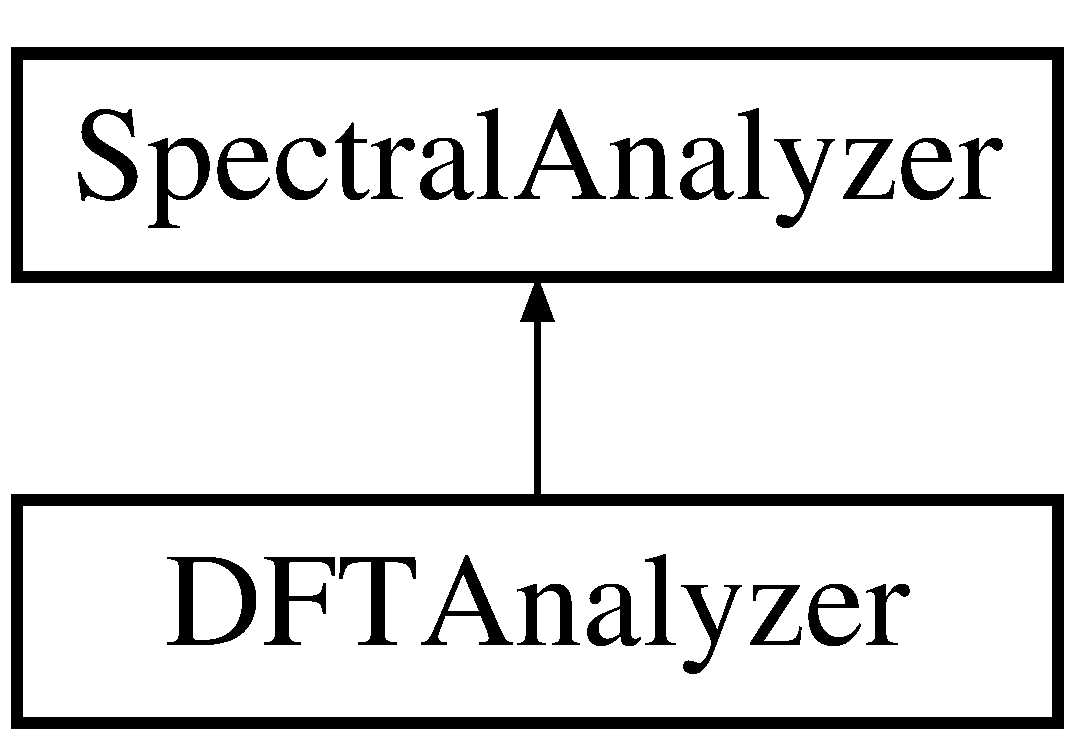
\includegraphics[height=2.000000cm]{class_d_f_t_analyzer}
\end{center}
\end{figure}
\subsection*{Public Member Functions}
\begin{DoxyCompactItemize}
\item 
\hyperlink{class_d_f_t_analyzer_a743ddb6bd928abc015f53eff23ce2c25}{D\+F\+T\+Analyzer} ()
\item 
\hyperlink{class_d_f_t_analyzer_ae7dec6c4824431056d2d171d8edf8cb6}{$\sim$\+D\+F\+T\+Analyzer} ()
\item 
void \hyperlink{class_d_f_t_analyzer_ad777180fdef8e09e0f2246ffd254fc14}{init} (unsigned int N, unsigned int overlap, \hyperlink{_utility_8h_a476342970f954b62d70552bcbb5ee509}{Window\+Type} t)
\item 
void \hyperlink{class_d_f_t_analyzer_a770f6798a76d08c346238c4f1d6e653a}{read\+And\+Analyse} (const float $\ast$input, long number\+Of\+Samples) override
\item 
void \hyperlink{class_d_f_t_analyzer_aa1882d12d45eea36098449bcf460c1de}{calculate\+Amplitudes} () override
\item 
void \hyperlink{class_d_f_t_analyzer_a92edf947d0ea4b4182d95510fabaeaaf}{calculate\+Phases} () override
\item 
void \hyperlink{class_d_f_t_analyzer_a4ccfe430f6137293c2b83a6954805959}{calculate\+Instant\+Frequencies} () override
\item 
void \hyperlink{class_d_f_t_analyzer_aa3faf80a26cab80412da95ffd482a266}{calculate\+Spectral\+Flux} ()
\item 
void \hyperlink{class_d_f_t_analyzer_ad497c408116b7e4b8650f45deaf25d58}{calculate\+Log\+Spectrum} ()
\item 
std\+::vector$<$ std\+::vector$<$ float $>$ $>$ \hyperlink{class_d_f_t_analyzer_a5b583b5c2c785e6cc76b6248f2efdd72}{get\+Amplitudes} ()
\item 
std\+::vector$<$ std\+::vector$<$ float $>$ $>$ \hyperlink{class_d_f_t_analyzer_ab24cf7ea52ffaf283395461569d9437e}{get\+Phases} ()
\item 
std\+::vector$<$ std\+::vector$<$ float $>$ $>$ \hyperlink{class_d_f_t_analyzer_a29d51cf796bb9a763f067ff913799f24}{get\+Frequenies} ()
\item 
std\+::vector$<$ float $>$ \hyperlink{class_d_f_t_analyzer_a18e4a463ee3b28f14c5c511243d8a551}{get\+Spectral\+Flux} ()
\end{DoxyCompactItemize}


\subsection{Constructor \& Destructor Documentation}
\hypertarget{class_d_f_t_analyzer_a743ddb6bd928abc015f53eff23ce2c25}{\index{D\+F\+T\+Analyzer@{D\+F\+T\+Analyzer}!D\+F\+T\+Analyzer@{D\+F\+T\+Analyzer}}
\index{D\+F\+T\+Analyzer@{D\+F\+T\+Analyzer}!D\+F\+T\+Analyzer@{D\+F\+T\+Analyzer}}
\subsubsection[{D\+F\+T\+Analyzer}]{\setlength{\rightskip}{0pt plus 5cm}D\+F\+T\+Analyzer\+::\+D\+F\+T\+Analyzer (
\begin{DoxyParamCaption}
{}
\end{DoxyParamCaption}
)}}\label{class_d_f_t_analyzer_a743ddb6bd928abc015f53eff23ce2c25}
\hypertarget{class_d_f_t_analyzer_ae7dec6c4824431056d2d171d8edf8cb6}{\index{D\+F\+T\+Analyzer@{D\+F\+T\+Analyzer}!````~D\+F\+T\+Analyzer@{$\sim$\+D\+F\+T\+Analyzer}}
\index{````~D\+F\+T\+Analyzer@{$\sim$\+D\+F\+T\+Analyzer}!D\+F\+T\+Analyzer@{D\+F\+T\+Analyzer}}
\subsubsection[{$\sim$\+D\+F\+T\+Analyzer}]{\setlength{\rightskip}{0pt plus 5cm}D\+F\+T\+Analyzer\+::$\sim$\+D\+F\+T\+Analyzer (
\begin{DoxyParamCaption}
{}
\end{DoxyParamCaption}
)}}\label{class_d_f_t_analyzer_ae7dec6c4824431056d2d171d8edf8cb6}


\subsection{Member Function Documentation}
\hypertarget{class_d_f_t_analyzer_aa1882d12d45eea36098449bcf460c1de}{\index{D\+F\+T\+Analyzer@{D\+F\+T\+Analyzer}!calculate\+Amplitudes@{calculate\+Amplitudes}}
\index{calculate\+Amplitudes@{calculate\+Amplitudes}!D\+F\+T\+Analyzer@{D\+F\+T\+Analyzer}}
\subsubsection[{calculate\+Amplitudes}]{\setlength{\rightskip}{0pt plus 5cm}void D\+F\+T\+Analyzer\+::calculate\+Amplitudes (
\begin{DoxyParamCaption}
{}
\end{DoxyParamCaption}
)\hspace{0.3cm}{\ttfamily [override]}, {\ttfamily [virtual]}}}\label{class_d_f_t_analyzer_aa1882d12d45eea36098449bcf460c1de}


Implements \hyperlink{class_spectral_analyzer_a78c2e37bef122ee6463023532abd0613}{Spectral\+Analyzer}.

\hypertarget{class_d_f_t_analyzer_a4ccfe430f6137293c2b83a6954805959}{\index{D\+F\+T\+Analyzer@{D\+F\+T\+Analyzer}!calculate\+Instant\+Frequencies@{calculate\+Instant\+Frequencies}}
\index{calculate\+Instant\+Frequencies@{calculate\+Instant\+Frequencies}!D\+F\+T\+Analyzer@{D\+F\+T\+Analyzer}}
\subsubsection[{calculate\+Instant\+Frequencies}]{\setlength{\rightskip}{0pt plus 5cm}void D\+F\+T\+Analyzer\+::calculate\+Instant\+Frequencies (
\begin{DoxyParamCaption}
{}
\end{DoxyParamCaption}
)\hspace{0.3cm}{\ttfamily [override]}, {\ttfamily [virtual]}}}\label{class_d_f_t_analyzer_a4ccfe430f6137293c2b83a6954805959}


Implements \hyperlink{class_spectral_analyzer_a0d3a2251d76a4083aec38b64af82b07e}{Spectral\+Analyzer}.

\hypertarget{class_d_f_t_analyzer_ad497c408116b7e4b8650f45deaf25d58}{\index{D\+F\+T\+Analyzer@{D\+F\+T\+Analyzer}!calculate\+Log\+Spectrum@{calculate\+Log\+Spectrum}}
\index{calculate\+Log\+Spectrum@{calculate\+Log\+Spectrum}!D\+F\+T\+Analyzer@{D\+F\+T\+Analyzer}}
\subsubsection[{calculate\+Log\+Spectrum}]{\setlength{\rightskip}{0pt plus 5cm}void D\+F\+T\+Analyzer\+::calculate\+Log\+Spectrum (
\begin{DoxyParamCaption}
{}
\end{DoxyParamCaption}
)}}\label{class_d_f_t_analyzer_ad497c408116b7e4b8650f45deaf25d58}
\hypertarget{class_d_f_t_analyzer_a92edf947d0ea4b4182d95510fabaeaaf}{\index{D\+F\+T\+Analyzer@{D\+F\+T\+Analyzer}!calculate\+Phases@{calculate\+Phases}}
\index{calculate\+Phases@{calculate\+Phases}!D\+F\+T\+Analyzer@{D\+F\+T\+Analyzer}}
\subsubsection[{calculate\+Phases}]{\setlength{\rightskip}{0pt plus 5cm}void D\+F\+T\+Analyzer\+::calculate\+Phases (
\begin{DoxyParamCaption}
{}
\end{DoxyParamCaption}
)\hspace{0.3cm}{\ttfamily [override]}, {\ttfamily [virtual]}}}\label{class_d_f_t_analyzer_a92edf947d0ea4b4182d95510fabaeaaf}


Implements \hyperlink{class_spectral_analyzer_a78d1748783b9597e6d1a3389db35c88f}{Spectral\+Analyzer}.

\hypertarget{class_d_f_t_analyzer_aa3faf80a26cab80412da95ffd482a266}{\index{D\+F\+T\+Analyzer@{D\+F\+T\+Analyzer}!calculate\+Spectral\+Flux@{calculate\+Spectral\+Flux}}
\index{calculate\+Spectral\+Flux@{calculate\+Spectral\+Flux}!D\+F\+T\+Analyzer@{D\+F\+T\+Analyzer}}
\subsubsection[{calculate\+Spectral\+Flux}]{\setlength{\rightskip}{0pt plus 5cm}void D\+F\+T\+Analyzer\+::calculate\+Spectral\+Flux (
\begin{DoxyParamCaption}
{}
\end{DoxyParamCaption}
)}}\label{class_d_f_t_analyzer_aa3faf80a26cab80412da95ffd482a266}
\hypertarget{class_d_f_t_analyzer_a5b583b5c2c785e6cc76b6248f2efdd72}{\index{D\+F\+T\+Analyzer@{D\+F\+T\+Analyzer}!get\+Amplitudes@{get\+Amplitudes}}
\index{get\+Amplitudes@{get\+Amplitudes}!D\+F\+T\+Analyzer@{D\+F\+T\+Analyzer}}
\subsubsection[{get\+Amplitudes}]{\setlength{\rightskip}{0pt plus 5cm}std\+::vector$<$std\+::vector$<$float$>$ $>$ D\+F\+T\+Analyzer\+::get\+Amplitudes (
\begin{DoxyParamCaption}
{}
\end{DoxyParamCaption}
)\hspace{0.3cm}{\ttfamily [inline]}}}\label{class_d_f_t_analyzer_a5b583b5c2c785e6cc76b6248f2efdd72}
\hypertarget{class_d_f_t_analyzer_a29d51cf796bb9a763f067ff913799f24}{\index{D\+F\+T\+Analyzer@{D\+F\+T\+Analyzer}!get\+Frequenies@{get\+Frequenies}}
\index{get\+Frequenies@{get\+Frequenies}!D\+F\+T\+Analyzer@{D\+F\+T\+Analyzer}}
\subsubsection[{get\+Frequenies}]{\setlength{\rightskip}{0pt plus 5cm}std\+::vector$<$std\+::vector$<$float$>$ $>$ D\+F\+T\+Analyzer\+::get\+Frequenies (
\begin{DoxyParamCaption}
{}
\end{DoxyParamCaption}
)\hspace{0.3cm}{\ttfamily [inline]}}}\label{class_d_f_t_analyzer_a29d51cf796bb9a763f067ff913799f24}
\hypertarget{class_d_f_t_analyzer_ab24cf7ea52ffaf283395461569d9437e}{\index{D\+F\+T\+Analyzer@{D\+F\+T\+Analyzer}!get\+Phases@{get\+Phases}}
\index{get\+Phases@{get\+Phases}!D\+F\+T\+Analyzer@{D\+F\+T\+Analyzer}}
\subsubsection[{get\+Phases}]{\setlength{\rightskip}{0pt plus 5cm}std\+::vector$<$std\+::vector$<$float$>$ $>$ D\+F\+T\+Analyzer\+::get\+Phases (
\begin{DoxyParamCaption}
{}
\end{DoxyParamCaption}
)\hspace{0.3cm}{\ttfamily [inline]}}}\label{class_d_f_t_analyzer_ab24cf7ea52ffaf283395461569d9437e}
\hypertarget{class_d_f_t_analyzer_a18e4a463ee3b28f14c5c511243d8a551}{\index{D\+F\+T\+Analyzer@{D\+F\+T\+Analyzer}!get\+Spectral\+Flux@{get\+Spectral\+Flux}}
\index{get\+Spectral\+Flux@{get\+Spectral\+Flux}!D\+F\+T\+Analyzer@{D\+F\+T\+Analyzer}}
\subsubsection[{get\+Spectral\+Flux}]{\setlength{\rightskip}{0pt plus 5cm}std\+::vector$<$float$>$ D\+F\+T\+Analyzer\+::get\+Spectral\+Flux (
\begin{DoxyParamCaption}
{}
\end{DoxyParamCaption}
)\hspace{0.3cm}{\ttfamily [inline]}}}\label{class_d_f_t_analyzer_a18e4a463ee3b28f14c5c511243d8a551}
\hypertarget{class_d_f_t_analyzer_ad777180fdef8e09e0f2246ffd254fc14}{\index{D\+F\+T\+Analyzer@{D\+F\+T\+Analyzer}!init@{init}}
\index{init@{init}!D\+F\+T\+Analyzer@{D\+F\+T\+Analyzer}}
\subsubsection[{init}]{\setlength{\rightskip}{0pt plus 5cm}void D\+F\+T\+Analyzer\+::init (
\begin{DoxyParamCaption}
\item[{unsigned int}]{N, }
\item[{unsigned int}]{overlap, }
\item[{{\bf Window\+Type}}]{t}
\end{DoxyParamCaption}
)}}\label{class_d_f_t_analyzer_ad777180fdef8e09e0f2246ffd254fc14}
\hypertarget{class_d_f_t_analyzer_a770f6798a76d08c346238c4f1d6e653a}{\index{D\+F\+T\+Analyzer@{D\+F\+T\+Analyzer}!read\+And\+Analyse@{read\+And\+Analyse}}
\index{read\+And\+Analyse@{read\+And\+Analyse}!D\+F\+T\+Analyzer@{D\+F\+T\+Analyzer}}
\subsubsection[{read\+And\+Analyse}]{\setlength{\rightskip}{0pt plus 5cm}void D\+F\+T\+Analyzer\+::read\+And\+Analyse (
\begin{DoxyParamCaption}
\item[{const float $\ast$}]{input, }
\item[{long}]{number\+Of\+Samples}
\end{DoxyParamCaption}
)\hspace{0.3cm}{\ttfamily [override]}, {\ttfamily [virtual]}}}\label{class_d_f_t_analyzer_a770f6798a76d08c346238c4f1d6e653a}


Implements \hyperlink{class_spectral_analyzer_a9d3c04321ce7c2066acfe03f5e172e4d}{Spectral\+Analyzer}.



The documentation for this class was generated from the following files\+:\begin{DoxyCompactItemize}
\item 
Analysis Classes/\+Headers/\hyperlink{_d_f_t_analyzer_8h}{D\+F\+T\+Analyzer.\+h}\item 
Analysis Classes/\+Implementations/\hyperlink{_d_f_t_analyzer_8cpp}{D\+F\+T\+Analyzer.\+cpp}\end{DoxyCompactItemize}

\hypertarget{class_d_f_t_spectogram}{\section{D\+F\+T\+Spectogram Class Reference}
\label{class_d_f_t_spectogram}\index{D\+F\+T\+Spectogram@{D\+F\+T\+Spectogram}}
}


{\ttfamily \#include $<$D\+F\+T\+Spectogram.\+h$>$}

Inheritance diagram for D\+F\+T\+Spectogram\+:\begin{figure}[H]
\begin{center}
\leavevmode
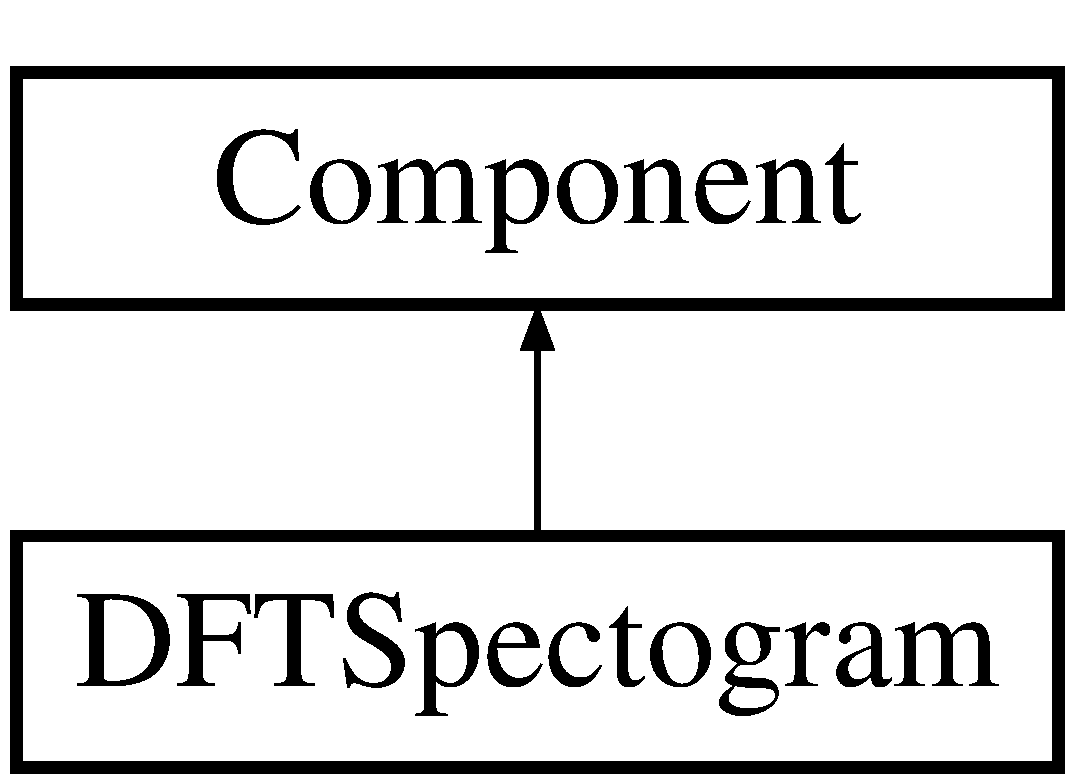
\includegraphics[height=2.000000cm]{class_d_f_t_spectogram}
\end{center}
\end{figure}
\subsection*{Public Member Functions}
\begin{DoxyCompactItemize}
\item 
\hyperlink{class_d_f_t_spectogram_aa5a17ff80308637394bbdd456382c6cf}{D\+F\+T\+Spectogram} (\hyperlink{class_a_p_audio_file_manager}{A\+P\+Audio\+File\+Manager} $\ast$file\+Manager, \hyperlink{class_d_f_t_analyzer}{D\+F\+T\+Analyzer} $\ast$analyzer)
\item 
\hyperlink{class_d_f_t_spectogram_a9bdf31e7f8d1a84b751a14f55e8b42db}{D\+F\+T\+Spectogram} ()
\item 
void \hyperlink{class_d_f_t_spectogram_a5bde5298e19b4396b07774a144935c12}{resized} () overridefinal
\item 
void \hyperlink{class_d_f_t_spectogram_a81348bfcec217526a83852865a374881}{paint} (Graphics \&g) overridefinal
\item 
void \hyperlink{class_d_f_t_spectogram_ae07e85a512f188d1127d37b2da39f535}{get\+Draw\+Data} (\hyperlink{class_a_p_audio_file}{A\+P\+Audio\+File} $\ast$audio\+File, int N, int window\+Size, int overlap)
\item 
void \hyperlink{class_d_f_t_spectogram_a033a0af0eec78479c480b72e96fed742}{mouse\+Up} (const Mouse\+Event \&event) overridefinal
\item 
void \hyperlink{class_d_f_t_spectogram_aeea5f226288e6005534f36b30835dd3e}{mouse\+Down} (const Mouse\+Event \&event) overridefinal
\end{DoxyCompactItemize}


\subsection{Constructor \& Destructor Documentation}
\hypertarget{class_d_f_t_spectogram_aa5a17ff80308637394bbdd456382c6cf}{\index{D\+F\+T\+Spectogram@{D\+F\+T\+Spectogram}!D\+F\+T\+Spectogram@{D\+F\+T\+Spectogram}}
\index{D\+F\+T\+Spectogram@{D\+F\+T\+Spectogram}!D\+F\+T\+Spectogram@{D\+F\+T\+Spectogram}}
\subsubsection[{D\+F\+T\+Spectogram}]{\setlength{\rightskip}{0pt plus 5cm}D\+F\+T\+Spectogram\+::\+D\+F\+T\+Spectogram (
\begin{DoxyParamCaption}
\item[{{\bf A\+P\+Audio\+File\+Manager} $\ast$}]{file\+Manager, }
\item[{{\bf D\+F\+T\+Analyzer} $\ast$}]{analyzer}
\end{DoxyParamCaption}
)}}\label{class_d_f_t_spectogram_aa5a17ff80308637394bbdd456382c6cf}
\hypertarget{class_d_f_t_spectogram_a9bdf31e7f8d1a84b751a14f55e8b42db}{\index{D\+F\+T\+Spectogram@{D\+F\+T\+Spectogram}!D\+F\+T\+Spectogram@{D\+F\+T\+Spectogram}}
\index{D\+F\+T\+Spectogram@{D\+F\+T\+Spectogram}!D\+F\+T\+Spectogram@{D\+F\+T\+Spectogram}}
\subsubsection[{D\+F\+T\+Spectogram}]{\setlength{\rightskip}{0pt plus 5cm}D\+F\+T\+Spectogram\+::\+D\+F\+T\+Spectogram (
\begin{DoxyParamCaption}
{}
\end{DoxyParamCaption}
)}}\label{class_d_f_t_spectogram_a9bdf31e7f8d1a84b751a14f55e8b42db}


\subsection{Member Function Documentation}
\hypertarget{class_d_f_t_spectogram_ae07e85a512f188d1127d37b2da39f535}{\index{D\+F\+T\+Spectogram@{D\+F\+T\+Spectogram}!get\+Draw\+Data@{get\+Draw\+Data}}
\index{get\+Draw\+Data@{get\+Draw\+Data}!D\+F\+T\+Spectogram@{D\+F\+T\+Spectogram}}
\subsubsection[{get\+Draw\+Data}]{\setlength{\rightskip}{0pt plus 5cm}void D\+F\+T\+Spectogram\+::get\+Draw\+Data (
\begin{DoxyParamCaption}
\item[{{\bf A\+P\+Audio\+File} $\ast$}]{audio\+File, }
\item[{int}]{N, }
\item[{int}]{window\+Size, }
\item[{int}]{overlap}
\end{DoxyParamCaption}
)}}\label{class_d_f_t_spectogram_ae07e85a512f188d1127d37b2da39f535}
\hypertarget{class_d_f_t_spectogram_aeea5f226288e6005534f36b30835dd3e}{\index{D\+F\+T\+Spectogram@{D\+F\+T\+Spectogram}!mouse\+Down@{mouse\+Down}}
\index{mouse\+Down@{mouse\+Down}!D\+F\+T\+Spectogram@{D\+F\+T\+Spectogram}}
\subsubsection[{mouse\+Down}]{\setlength{\rightskip}{0pt plus 5cm}void D\+F\+T\+Spectogram\+::mouse\+Down (
\begin{DoxyParamCaption}
\item[{const Mouse\+Event \&}]{event}
\end{DoxyParamCaption}
)\hspace{0.3cm}{\ttfamily [final]}, {\ttfamily [override]}}}\label{class_d_f_t_spectogram_aeea5f226288e6005534f36b30835dd3e}
\hypertarget{class_d_f_t_spectogram_a033a0af0eec78479c480b72e96fed742}{\index{D\+F\+T\+Spectogram@{D\+F\+T\+Spectogram}!mouse\+Up@{mouse\+Up}}
\index{mouse\+Up@{mouse\+Up}!D\+F\+T\+Spectogram@{D\+F\+T\+Spectogram}}
\subsubsection[{mouse\+Up}]{\setlength{\rightskip}{0pt plus 5cm}void D\+F\+T\+Spectogram\+::mouse\+Up (
\begin{DoxyParamCaption}
\item[{const Mouse\+Event \&}]{event}
\end{DoxyParamCaption}
)\hspace{0.3cm}{\ttfamily [final]}, {\ttfamily [override]}}}\label{class_d_f_t_spectogram_a033a0af0eec78479c480b72e96fed742}
\hypertarget{class_d_f_t_spectogram_a81348bfcec217526a83852865a374881}{\index{D\+F\+T\+Spectogram@{D\+F\+T\+Spectogram}!paint@{paint}}
\index{paint@{paint}!D\+F\+T\+Spectogram@{D\+F\+T\+Spectogram}}
\subsubsection[{paint}]{\setlength{\rightskip}{0pt plus 5cm}void D\+F\+T\+Spectogram\+::paint (
\begin{DoxyParamCaption}
\item[{Graphics \&}]{g}
\end{DoxyParamCaption}
)\hspace{0.3cm}{\ttfamily [final]}, {\ttfamily [override]}}}\label{class_d_f_t_spectogram_a81348bfcec217526a83852865a374881}
\hypertarget{class_d_f_t_spectogram_a5bde5298e19b4396b07774a144935c12}{\index{D\+F\+T\+Spectogram@{D\+F\+T\+Spectogram}!resized@{resized}}
\index{resized@{resized}!D\+F\+T\+Spectogram@{D\+F\+T\+Spectogram}}
\subsubsection[{resized}]{\setlength{\rightskip}{0pt plus 5cm}void D\+F\+T\+Spectogram\+::resized (
\begin{DoxyParamCaption}
{}
\end{DoxyParamCaption}
)\hspace{0.3cm}{\ttfamily [final]}, {\ttfamily [override]}}}\label{class_d_f_t_spectogram_a5bde5298e19b4396b07774a144935c12}


The documentation for this class was generated from the following files\+:\begin{DoxyCompactItemize}
\item 
G\+U\+I Classes/\+Headers/\hyperlink{_d_f_t_spectogram_8h}{D\+F\+T\+Spectogram.\+h}\item 
G\+U\+I Classes/\+Implementations/\hyperlink{_d_f_t_spectogram_8cpp}{D\+F\+T\+Spectogram.\+cpp}\end{DoxyCompactItemize}

\hypertarget{class_fast_wavelet}{\section{Fast\+Wavelet Class Reference}
\label{class_fast_wavelet}\index{Fast\+Wavelet@{Fast\+Wavelet}}
}


{\ttfamily \#include $<$Fast\+Wavelet.\+h$>$}

\subsection*{Public Member Functions}
\begin{DoxyCompactItemize}
\item 
\hyperlink{class_fast_wavelet_abaf95595befd9514c356965b031ee4a1}{Fast\+Wavelet} ()
\item 
void \hyperlink{class_fast_wavelet_a46714dff2b93deae50ba0bbf93abdeb6}{process} (float $\ast$input, unsigned int N, int direction)
\end{DoxyCompactItemize}


\subsection{Constructor \& Destructor Documentation}
\hypertarget{class_fast_wavelet_abaf95595befd9514c356965b031ee4a1}{\index{Fast\+Wavelet@{Fast\+Wavelet}!Fast\+Wavelet@{Fast\+Wavelet}}
\index{Fast\+Wavelet@{Fast\+Wavelet}!Fast\+Wavelet@{Fast\+Wavelet}}
\subsubsection[{Fast\+Wavelet}]{\setlength{\rightskip}{0pt plus 5cm}Fast\+Wavelet\+::\+Fast\+Wavelet (
\begin{DoxyParamCaption}
{}
\end{DoxyParamCaption}
)}}\label{class_fast_wavelet_abaf95595befd9514c356965b031ee4a1}


\subsection{Member Function Documentation}
\hypertarget{class_fast_wavelet_a46714dff2b93deae50ba0bbf93abdeb6}{\index{Fast\+Wavelet@{Fast\+Wavelet}!process@{process}}
\index{process@{process}!Fast\+Wavelet@{Fast\+Wavelet}}
\subsubsection[{process}]{\setlength{\rightskip}{0pt plus 5cm}void Fast\+Wavelet\+::process (
\begin{DoxyParamCaption}
\item[{float $\ast$}]{input, }
\item[{unsigned int}]{N, }
\item[{int}]{direction}
\end{DoxyParamCaption}
)}}\label{class_fast_wavelet_a46714dff2b93deae50ba0bbf93abdeb6}


The documentation for this class was generated from the following files\+:\begin{DoxyCompactItemize}
\item 
Analysis Classes/\+Headers/\hyperlink{_fast_wavelet_8h}{Fast\+Wavelet.\+h}\item 
Analysis Classes/\+Implementations/\hyperlink{_fast_wavelet_8cpp}{Fast\+Wavelet.\+cpp}\end{DoxyCompactItemize}

\hypertarget{class_fast_wavelet_analyzer}{\section{Fast\+Wavelet\+Analyzer Class Reference}
\label{class_fast_wavelet_analyzer}\index{Fast\+Wavelet\+Analyzer@{Fast\+Wavelet\+Analyzer}}
}


{\ttfamily \#include $<$Fast\+Wavelet\+Analyzer.\+h$>$}

Inheritance diagram for Fast\+Wavelet\+Analyzer\+:\begin{figure}[H]
\begin{center}
\leavevmode
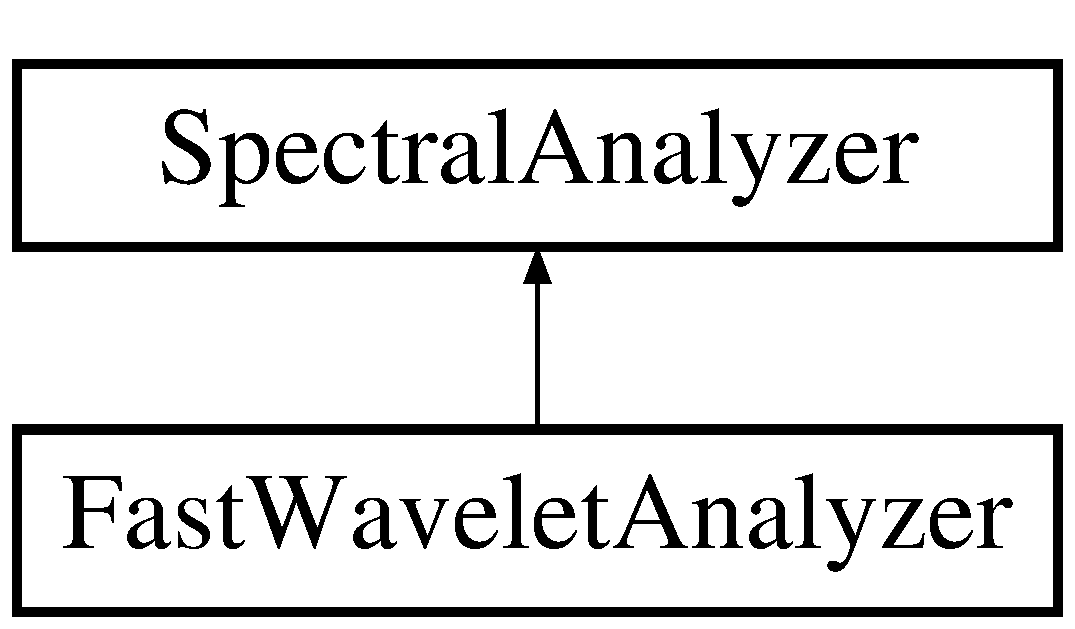
\includegraphics[height=2.000000cm]{class_fast_wavelet_analyzer}
\end{center}
\end{figure}
\subsection*{Public Member Functions}
\begin{DoxyCompactItemize}
\item 
\hyperlink{class_fast_wavelet_analyzer_ab7883d282ec0866f3c1660f475eea767}{Fast\+Wavelet\+Analyzer} (unsigned int N, unsigned int overlap)
\item 
\hyperlink{class_fast_wavelet_analyzer_ac24b3e5df3fcb69212211bc0d70a067d}{$\sim$\+Fast\+Wavelet\+Analyzer} ()
\end{DoxyCompactItemize}


\subsection{Constructor \& Destructor Documentation}
\hypertarget{class_fast_wavelet_analyzer_ab7883d282ec0866f3c1660f475eea767}{\index{Fast\+Wavelet\+Analyzer@{Fast\+Wavelet\+Analyzer}!Fast\+Wavelet\+Analyzer@{Fast\+Wavelet\+Analyzer}}
\index{Fast\+Wavelet\+Analyzer@{Fast\+Wavelet\+Analyzer}!Fast\+Wavelet\+Analyzer@{Fast\+Wavelet\+Analyzer}}
\subsubsection[{Fast\+Wavelet\+Analyzer}]{\setlength{\rightskip}{0pt plus 5cm}Fast\+Wavelet\+Analyzer\+::\+Fast\+Wavelet\+Analyzer (
\begin{DoxyParamCaption}
\item[{unsigned int}]{N, }
\item[{unsigned int}]{overlap}
\end{DoxyParamCaption}
)}}\label{class_fast_wavelet_analyzer_ab7883d282ec0866f3c1660f475eea767}
\hypertarget{class_fast_wavelet_analyzer_ac24b3e5df3fcb69212211bc0d70a067d}{\index{Fast\+Wavelet\+Analyzer@{Fast\+Wavelet\+Analyzer}!````~Fast\+Wavelet\+Analyzer@{$\sim$\+Fast\+Wavelet\+Analyzer}}
\index{````~Fast\+Wavelet\+Analyzer@{$\sim$\+Fast\+Wavelet\+Analyzer}!Fast\+Wavelet\+Analyzer@{Fast\+Wavelet\+Analyzer}}
\subsubsection[{$\sim$\+Fast\+Wavelet\+Analyzer}]{\setlength{\rightskip}{0pt plus 5cm}Fast\+Wavelet\+Analyzer\+::$\sim$\+Fast\+Wavelet\+Analyzer (
\begin{DoxyParamCaption}
{}
\end{DoxyParamCaption}
)}}\label{class_fast_wavelet_analyzer_ac24b3e5df3fcb69212211bc0d70a067d}


The documentation for this class was generated from the following files\+:\begin{DoxyCompactItemize}
\item 
Analysis Classes/\+Headers/\hyperlink{_fast_wavelet_analyzer_8h}{Fast\+Wavelet\+Analyzer.\+h}\item 
Analysis Classes/\+Implementations/\hyperlink{_fast_wavelet_analyzer_8cpp}{Fast\+Wavelet\+Analyzer.\+cpp}\end{DoxyCompactItemize}

\hypertarget{class_frequency_analyzer}{\section{Frequency\+Analyzer Class Reference}
\label{class_frequency_analyzer}\index{Frequency\+Analyzer@{Frequency\+Analyzer}}
}


{\ttfamily \#include $<$Frequency\+Analyzer.\+h$>$}

\subsection*{Public Member Functions}
\begin{DoxyCompactItemize}
\item 
\hyperlink{class_frequency_analyzer_ac4599ecb88556d2b219d60c363cb35c8}{Frequency\+Analyzer} (int N)
\item 
void \hyperlink{class_frequency_analyzer_ac84c6aa195c7c5ad0e132bf48d0999ff}{read\+And\+Analyse} (const float $\ast$input, long int number\+Of\+Samples)
\item 
std\+::vector$<$ float $>$ \hyperlink{class_frequency_analyzer_a5273f7ab3c5da77375a05e82f04dc91d}{get\+Result} ()
\end{DoxyCompactItemize}


\subsection{Constructor \& Destructor Documentation}
\hypertarget{class_frequency_analyzer_ac4599ecb88556d2b219d60c363cb35c8}{\index{Frequency\+Analyzer@{Frequency\+Analyzer}!Frequency\+Analyzer@{Frequency\+Analyzer}}
\index{Frequency\+Analyzer@{Frequency\+Analyzer}!Frequency\+Analyzer@{Frequency\+Analyzer}}
\subsubsection[{Frequency\+Analyzer}]{\setlength{\rightskip}{0pt plus 5cm}Frequency\+Analyzer\+::\+Frequency\+Analyzer (
\begin{DoxyParamCaption}
\item[{int}]{N}
\end{DoxyParamCaption}
)}}\label{class_frequency_analyzer_ac4599ecb88556d2b219d60c363cb35c8}


\subsection{Member Function Documentation}
\hypertarget{class_frequency_analyzer_a5273f7ab3c5da77375a05e82f04dc91d}{\index{Frequency\+Analyzer@{Frequency\+Analyzer}!get\+Result@{get\+Result}}
\index{get\+Result@{get\+Result}!Frequency\+Analyzer@{Frequency\+Analyzer}}
\subsubsection[{get\+Result}]{\setlength{\rightskip}{0pt plus 5cm}std\+::vector$<$float$>$ Frequency\+Analyzer\+::get\+Result (
\begin{DoxyParamCaption}
{}
\end{DoxyParamCaption}
)\hspace{0.3cm}{\ttfamily [inline]}}}\label{class_frequency_analyzer_a5273f7ab3c5da77375a05e82f04dc91d}
\hypertarget{class_frequency_analyzer_ac84c6aa195c7c5ad0e132bf48d0999ff}{\index{Frequency\+Analyzer@{Frequency\+Analyzer}!read\+And\+Analyse@{read\+And\+Analyse}}
\index{read\+And\+Analyse@{read\+And\+Analyse}!Frequency\+Analyzer@{Frequency\+Analyzer}}
\subsubsection[{read\+And\+Analyse}]{\setlength{\rightskip}{0pt plus 5cm}void Frequency\+Analyzer\+::read\+And\+Analyse (
\begin{DoxyParamCaption}
\item[{const float $\ast$}]{input, }
\item[{long int}]{number\+Of\+Samples}
\end{DoxyParamCaption}
)}}\label{class_frequency_analyzer_ac84c6aa195c7c5ad0e132bf48d0999ff}


The documentation for this class was generated from the following files\+:\begin{DoxyCompactItemize}
\item 
Analysis Classes/\+Headers/\hyperlink{_frequency_analyzer_8h}{Frequency\+Analyzer.\+h}\item 
Analysis Classes/\+Implementations/\hyperlink{_frequency_analyzer_8cpp}{Frequency\+Analyzer.\+cpp}\end{DoxyCompactItemize}

\hypertarget{struct_gyrometer_data}{\section{Gyrometer\+Data Struct Reference}
\label{struct_gyrometer_data}\index{Gyrometer\+Data@{Gyrometer\+Data}}
}


{\ttfamily \#include $<$Acceleration.\+h$>$}

\subsection*{Public Attributes}
\begin{DoxyCompactItemize}
\item 
float \hyperlink{struct_gyrometer_data_aa41d623b1e9547c10ee44159a6d5db1f}{x}
\item 
float \hyperlink{struct_gyrometer_data_a8bfd159a6f023fd90396425f23acb52d}{y}
\item 
float \hyperlink{struct_gyrometer_data_aef98320fd8b42a60a7bb8b424bea6f62}{z}
\end{DoxyCompactItemize}


\subsection{Member Data Documentation}
\hypertarget{struct_gyrometer_data_aa41d623b1e9547c10ee44159a6d5db1f}{\index{Gyrometer\+Data@{Gyrometer\+Data}!x@{x}}
\index{x@{x}!Gyrometer\+Data@{Gyrometer\+Data}}
\subsubsection[{x}]{\setlength{\rightskip}{0pt plus 5cm}float Gyrometer\+Data\+::x}}\label{struct_gyrometer_data_aa41d623b1e9547c10ee44159a6d5db1f}
\hypertarget{struct_gyrometer_data_a8bfd159a6f023fd90396425f23acb52d}{\index{Gyrometer\+Data@{Gyrometer\+Data}!y@{y}}
\index{y@{y}!Gyrometer\+Data@{Gyrometer\+Data}}
\subsubsection[{y}]{\setlength{\rightskip}{0pt plus 5cm}float Gyrometer\+Data\+::y}}\label{struct_gyrometer_data_a8bfd159a6f023fd90396425f23acb52d}
\hypertarget{struct_gyrometer_data_aef98320fd8b42a60a7bb8b424bea6f62}{\index{Gyrometer\+Data@{Gyrometer\+Data}!z@{z}}
\index{z@{z}!Gyrometer\+Data@{Gyrometer\+Data}}
\subsubsection[{z}]{\setlength{\rightskip}{0pt plus 5cm}float Gyrometer\+Data\+::z}}\label{struct_gyrometer_data_aef98320fd8b42a60a7bb8b424bea6f62}


The documentation for this struct was generated from the following file\+:\begin{DoxyCompactItemize}
\item 
i\+O\+S\+Sensor\+Wrappers/\+Headers/\hyperlink{_acceleration_8h}{Acceleration.\+h}\end{DoxyCompactItemize}

\hypertarget{class_multi_resolution_transform}{\section{Multi\+Resolution\+Transform Class Reference}
\label{class_multi_resolution_transform}\index{Multi\+Resolution\+Transform@{Multi\+Resolution\+Transform}}
}


{\ttfamily \#include $<$Multi\+Resolution\+Transform.\+h$>$}

Inheritance diagram for Multi\+Resolution\+Transform\+:\begin{figure}[H]
\begin{center}
\leavevmode
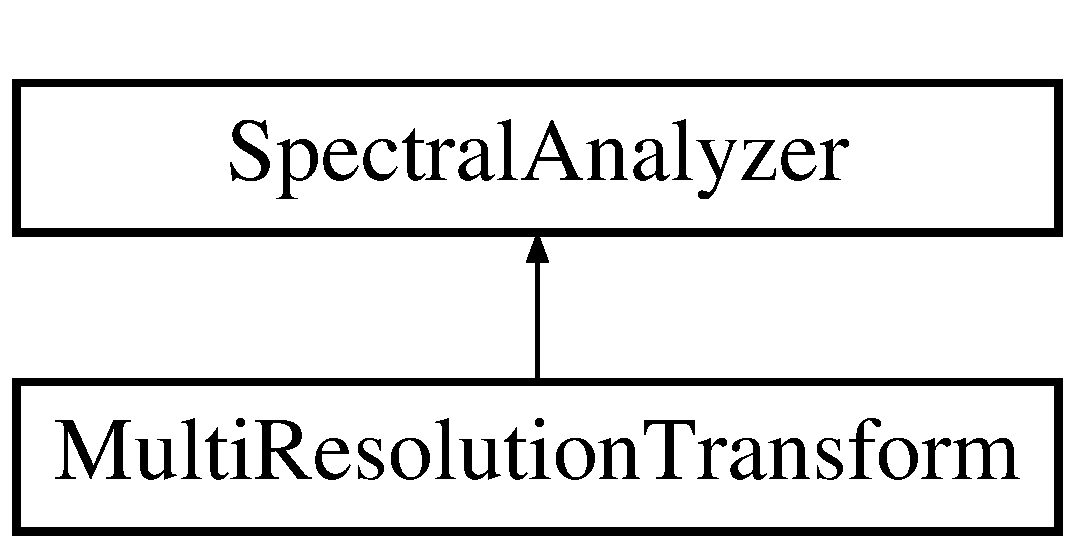
\includegraphics[height=2.000000cm]{class_multi_resolution_transform}
\end{center}
\end{figure}
\subsection*{Public Member Functions}
\begin{DoxyCompactItemize}
\item 
\hyperlink{class_multi_resolution_transform_a1b187ef11930f35eb94eb1e0eca2ba2c}{Multi\+Resolution\+Transform} (unsigned int N, unsigned int overlap)
\item 
\hyperlink{class_multi_resolution_transform_a995b7dbca27bbcde4a7e4a7436ab2469}{$\sim$\+Multi\+Resolution\+Transform} ()
\end{DoxyCompactItemize}


\subsection{Constructor \& Destructor Documentation}
\hypertarget{class_multi_resolution_transform_a1b187ef11930f35eb94eb1e0eca2ba2c}{\index{Multi\+Resolution\+Transform@{Multi\+Resolution\+Transform}!Multi\+Resolution\+Transform@{Multi\+Resolution\+Transform}}
\index{Multi\+Resolution\+Transform@{Multi\+Resolution\+Transform}!Multi\+Resolution\+Transform@{Multi\+Resolution\+Transform}}
\subsubsection[{Multi\+Resolution\+Transform}]{\setlength{\rightskip}{0pt plus 5cm}Multi\+Resolution\+Transform\+::\+Multi\+Resolution\+Transform (
\begin{DoxyParamCaption}
\item[{unsigned int}]{N, }
\item[{unsigned int}]{overlap}
\end{DoxyParamCaption}
)}}\label{class_multi_resolution_transform_a1b187ef11930f35eb94eb1e0eca2ba2c}
\hypertarget{class_multi_resolution_transform_a995b7dbca27bbcde4a7e4a7436ab2469}{\index{Multi\+Resolution\+Transform@{Multi\+Resolution\+Transform}!````~Multi\+Resolution\+Transform@{$\sim$\+Multi\+Resolution\+Transform}}
\index{````~Multi\+Resolution\+Transform@{$\sim$\+Multi\+Resolution\+Transform}!Multi\+Resolution\+Transform@{Multi\+Resolution\+Transform}}
\subsubsection[{$\sim$\+Multi\+Resolution\+Transform}]{\setlength{\rightskip}{0pt plus 5cm}Multi\+Resolution\+Transform\+::$\sim$\+Multi\+Resolution\+Transform (
\begin{DoxyParamCaption}
{}
\end{DoxyParamCaption}
)}}\label{class_multi_resolution_transform_a995b7dbca27bbcde4a7e4a7436ab2469}


The documentation for this class was generated from the following files\+:\begin{DoxyCompactItemize}
\item 
Analysis Classes/\+Headers/\hyperlink{_multi_resolution_transform_8h}{Multi\+Resolution\+Transform.\+h}\item 
Analysis Classes/\+Implementations/\hyperlink{_multi_resolution_transform_8cpp}{Multi\+Resolution\+Transform.\+cpp}\end{DoxyCompactItemize}

\hypertarget{class_sampler}{\section{Sampler Class Reference}
\label{class_sampler}\index{Sampler@{Sampler}}
}


{\ttfamily \#include $<$A\+P\+Audio\+Sampler.\+h$>$}

Inheritance diagram for Sampler\+:\begin{figure}[H]
\begin{center}
\leavevmode
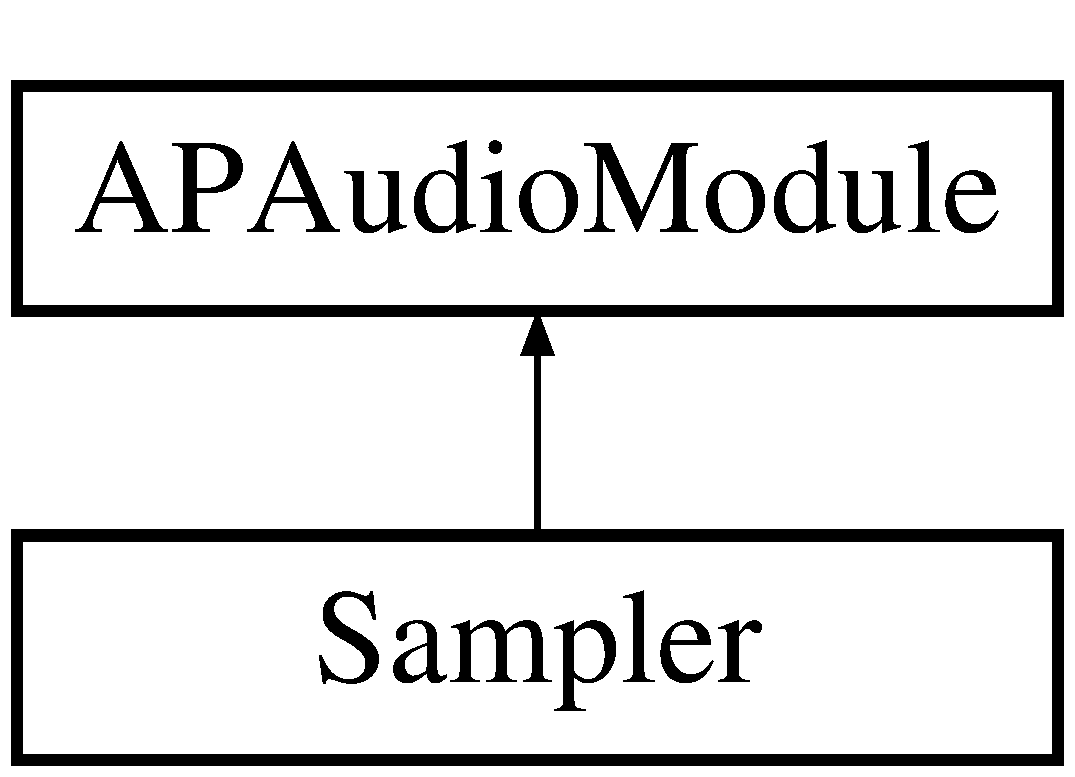
\includegraphics[height=2.000000cm]{class_sampler}
\end{center}
\end{figure}
\subsection*{Public Member Functions}
\begin{DoxyCompactItemize}
\item 
\hyperlink{class_sampler_a4b1dae034b5a62d1111755ad575d520c}{Sampler} (\hyperlink{class_a_p_audio_main_frame}{A\+P\+Audio\+Main\+Frame} $\ast$main\+Frame, \hyperlink{class_a_p_audio_file_manager}{A\+P\+Audio\+File\+Manager} $\ast$file\+Manager)
\item 
\hyperlink{class_sampler_afbbbd238b78dd3024686c852b69fa64e}{$\sim$\+Sampler} ()
\item 
void \hyperlink{class_sampler_a59179aef89faa7fecccfed899a813a39}{on\+Note\+On} (int note\+On, float velocity, int channel, bool repeat)
\item 
\hyperlink{class_a_p_audio_sampler_voice}{A\+P\+Audio\+Sampler\+Voice} $\ast$ \hyperlink{class_sampler_af1cdbecc6b56d2f66f210919b70b4e9d}{find\+Free\+Voice} ()
\item 
void \hyperlink{class_sampler_a8eccc70de85144edcbae1d07ec148f25}{render\+Block} (\hyperlink{_a_p_audio_module_8h_a2c2f997fdc6b0e88b3723fb20dc502f0}{Sample\+Buffer} output)
\item 
void \hyperlink{class_sampler_a7cfe609d13791602b08426f639d47c70}{load\+File} (std\+::string file\+To\+Load, int note\+To\+Listen\+To, int channel\+To\+Listen\+To)
\item 
void \hyperlink{class_sampler_a1229142ba0a49229553e2cf1a525274d}{calculate\+Buffer} () override
\item 
void \hyperlink{class_sampler_afa02ace7d8c1c8e1890cb91f705a4579}{set\+Speed} (float speed)
\item 
void \hyperlink{class_sampler_a5f746f60864163e805bd8c8f198b1a29}{set\+Voice\+Amplitude} (int voice, float amp)
\end{DoxyCompactItemize}
\subsection*{Additional Inherited Members}


\subsection{Constructor \& Destructor Documentation}
\hypertarget{class_sampler_a4b1dae034b5a62d1111755ad575d520c}{\index{Sampler@{Sampler}!Sampler@{Sampler}}
\index{Sampler@{Sampler}!Sampler@{Sampler}}
\subsubsection[{Sampler}]{\setlength{\rightskip}{0pt plus 5cm}Sampler\+::\+Sampler (
\begin{DoxyParamCaption}
\item[{{\bf A\+P\+Audio\+Main\+Frame} $\ast$}]{main\+Frame, }
\item[{{\bf A\+P\+Audio\+File\+Manager} $\ast$}]{file\+Manager}
\end{DoxyParamCaption}
)}}\label{class_sampler_a4b1dae034b5a62d1111755ad575d520c}
\hypertarget{class_sampler_afbbbd238b78dd3024686c852b69fa64e}{\index{Sampler@{Sampler}!````~Sampler@{$\sim$\+Sampler}}
\index{````~Sampler@{$\sim$\+Sampler}!Sampler@{Sampler}}
\subsubsection[{$\sim$\+Sampler}]{\setlength{\rightskip}{0pt plus 5cm}Sampler\+::$\sim$\+Sampler (
\begin{DoxyParamCaption}
{}
\end{DoxyParamCaption}
)}}\label{class_sampler_afbbbd238b78dd3024686c852b69fa64e}


\subsection{Member Function Documentation}
\hypertarget{class_sampler_a1229142ba0a49229553e2cf1a525274d}{\index{Sampler@{Sampler}!calculate\+Buffer@{calculate\+Buffer}}
\index{calculate\+Buffer@{calculate\+Buffer}!Sampler@{Sampler}}
\subsubsection[{calculate\+Buffer}]{\setlength{\rightskip}{0pt plus 5cm}void Sampler\+::calculate\+Buffer (
\begin{DoxyParamCaption}
{}
\end{DoxyParamCaption}
)\hspace{0.3cm}{\ttfamily [override]}, {\ttfamily [virtual]}}}\label{class_sampler_a1229142ba0a49229553e2cf1a525274d}


Reimplemented from \hyperlink{class_a_p_audio_module_a10c6d7f469b9d1626a80c4d745663a2a}{A\+P\+Audio\+Module}.

\hypertarget{class_sampler_af1cdbecc6b56d2f66f210919b70b4e9d}{\index{Sampler@{Sampler}!find\+Free\+Voice@{find\+Free\+Voice}}
\index{find\+Free\+Voice@{find\+Free\+Voice}!Sampler@{Sampler}}
\subsubsection[{find\+Free\+Voice}]{\setlength{\rightskip}{0pt plus 5cm}{\bf A\+P\+Audio\+Sampler\+Voice} $\ast$ Sampler\+::find\+Free\+Voice (
\begin{DoxyParamCaption}
{}
\end{DoxyParamCaption}
)}}\label{class_sampler_af1cdbecc6b56d2f66f210919b70b4e9d}
\hypertarget{class_sampler_a7cfe609d13791602b08426f639d47c70}{\index{Sampler@{Sampler}!load\+File@{load\+File}}
\index{load\+File@{load\+File}!Sampler@{Sampler}}
\subsubsection[{load\+File}]{\setlength{\rightskip}{0pt plus 5cm}void Sampler\+::load\+File (
\begin{DoxyParamCaption}
\item[{std\+::string}]{file\+To\+Load, }
\item[{int}]{note\+To\+Listen\+To, }
\item[{int}]{channel\+To\+Listen\+To}
\end{DoxyParamCaption}
)}}\label{class_sampler_a7cfe609d13791602b08426f639d47c70}
\hypertarget{class_sampler_a59179aef89faa7fecccfed899a813a39}{\index{Sampler@{Sampler}!on\+Note\+On@{on\+Note\+On}}
\index{on\+Note\+On@{on\+Note\+On}!Sampler@{Sampler}}
\subsubsection[{on\+Note\+On}]{\setlength{\rightskip}{0pt plus 5cm}void Sampler\+::on\+Note\+On (
\begin{DoxyParamCaption}
\item[{int}]{note\+On, }
\item[{float}]{velocity, }
\item[{int}]{channel, }
\item[{bool}]{repeat}
\end{DoxyParamCaption}
)}}\label{class_sampler_a59179aef89faa7fecccfed899a813a39}
\hypertarget{class_sampler_a8eccc70de85144edcbae1d07ec148f25}{\index{Sampler@{Sampler}!render\+Block@{render\+Block}}
\index{render\+Block@{render\+Block}!Sampler@{Sampler}}
\subsubsection[{render\+Block}]{\setlength{\rightskip}{0pt plus 5cm}void Sampler\+::render\+Block (
\begin{DoxyParamCaption}
\item[{{\bf Sample\+Buffer}}]{output}
\end{DoxyParamCaption}
)}}\label{class_sampler_a8eccc70de85144edcbae1d07ec148f25}
\hypertarget{class_sampler_afa02ace7d8c1c8e1890cb91f705a4579}{\index{Sampler@{Sampler}!set\+Speed@{set\+Speed}}
\index{set\+Speed@{set\+Speed}!Sampler@{Sampler}}
\subsubsection[{set\+Speed}]{\setlength{\rightskip}{0pt plus 5cm}void Sampler\+::set\+Speed (
\begin{DoxyParamCaption}
\item[{float}]{speed}
\end{DoxyParamCaption}
)}}\label{class_sampler_afa02ace7d8c1c8e1890cb91f705a4579}
\hypertarget{class_sampler_a5f746f60864163e805bd8c8f198b1a29}{\index{Sampler@{Sampler}!set\+Voice\+Amplitude@{set\+Voice\+Amplitude}}
\index{set\+Voice\+Amplitude@{set\+Voice\+Amplitude}!Sampler@{Sampler}}
\subsubsection[{set\+Voice\+Amplitude}]{\setlength{\rightskip}{0pt plus 5cm}void Sampler\+::set\+Voice\+Amplitude (
\begin{DoxyParamCaption}
\item[{int}]{voice, }
\item[{float}]{amp}
\end{DoxyParamCaption}
)}}\label{class_sampler_a5f746f60864163e805bd8c8f198b1a29}


The documentation for this class was generated from the following files\+:\begin{DoxyCompactItemize}
\item 
Audio Classes/\+Headers/\hyperlink{_a_p_audio_sampler_8h}{A\+P\+Audio\+Sampler.\+h}\item 
Audio Classes/\+Implementations/\hyperlink{_a_p_audio_sampler_8cpp}{A\+P\+Audio\+Sampler.\+cpp}\end{DoxyCompactItemize}

\hypertarget{class_spectral_analyzer}{\section{Spectral\+Analyzer Class Reference}
\label{class_spectral_analyzer}\index{Spectral\+Analyzer@{Spectral\+Analyzer}}
}


{\ttfamily \#include $<$Spectral\+Analyzer.\+h$>$}

Inheritance diagram for Spectral\+Analyzer\+:\begin{figure}[H]
\begin{center}
\leavevmode
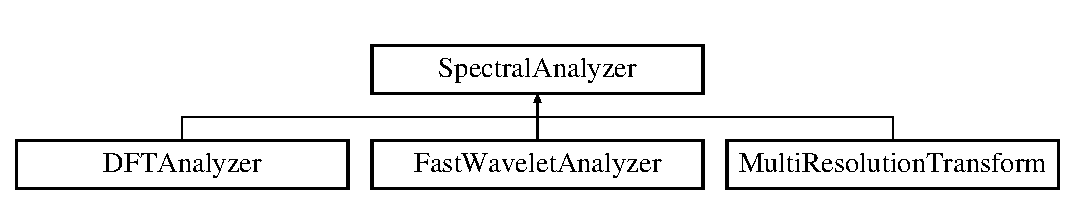
\includegraphics[height=2.000000cm]{class_spectral_analyzer}
\end{center}
\end{figure}
\subsection*{Public Member Functions}
\begin{DoxyCompactItemize}
\item 
\hyperlink{class_spectral_analyzer_a4f1f8101066e641d76af29dbafe2ffc4}{Spectral\+Analyzer} ()
\item 
virtual \hyperlink{class_spectral_analyzer_af15c01ed65303bf3dfd736384fcf6c2b}{$\sim$\+Spectral\+Analyzer} ()=0
\item 
virtual void \hyperlink{class_spectral_analyzer_a9d3c04321ce7c2066acfe03f5e172e4d}{read\+And\+Analyse} (const float $\ast$input, long number\+Of\+Samples)=0
\item 
virtual void \hyperlink{class_spectral_analyzer_a78d1748783b9597e6d1a3389db35c88f}{calculate\+Phases} ()=0
\item 
virtual void \hyperlink{class_spectral_analyzer_a78c2e37bef122ee6463023532abd0613}{calculate\+Amplitudes} ()=0
\item 
virtual void \hyperlink{class_spectral_analyzer_a0d3a2251d76a4083aec38b64af82b07e}{calculate\+Instant\+Frequencies} ()=0
\item 
void \hyperlink{class_spectral_analyzer_a23db8cab6892758fabc4cb779a315b96}{set\+Hopsize} (int hop\+Size)
\item 
void \hyperlink{class_spectral_analyzer_a4009ad3b900d4bc4539f76fa4dff088e}{set\+N} (int N)
\item 
void \hyperlink{class_spectral_analyzer_aa2bedb0e6e0370c2492b8d225f020b10}{set\+Overlap} (int N)
\item 
int \hyperlink{class_spectral_analyzer_afc9cfa190b98ddc1176d8ace6158c490}{get\+Hopsize} ()
\item 
int \hyperlink{class_spectral_analyzer_a87075bcd7cf8cc4c0a4729f8ed3f86c0}{get\+Window\+Size} ()
\item 
int \hyperlink{class_spectral_analyzer_a205d6ff6464ccf510afd9a7c3429276f}{get\+Overlap} ()
\end{DoxyCompactItemize}


\subsection{Constructor \& Destructor Documentation}
\hypertarget{class_spectral_analyzer_a4f1f8101066e641d76af29dbafe2ffc4}{\index{Spectral\+Analyzer@{Spectral\+Analyzer}!Spectral\+Analyzer@{Spectral\+Analyzer}}
\index{Spectral\+Analyzer@{Spectral\+Analyzer}!Spectral\+Analyzer@{Spectral\+Analyzer}}
\subsubsection[{Spectral\+Analyzer}]{\setlength{\rightskip}{0pt plus 5cm}Spectral\+Analyzer\+::\+Spectral\+Analyzer (
\begin{DoxyParamCaption}
{}
\end{DoxyParamCaption}
)}}\label{class_spectral_analyzer_a4f1f8101066e641d76af29dbafe2ffc4}
\hypertarget{class_spectral_analyzer_af15c01ed65303bf3dfd736384fcf6c2b}{\index{Spectral\+Analyzer@{Spectral\+Analyzer}!````~Spectral\+Analyzer@{$\sim$\+Spectral\+Analyzer}}
\index{````~Spectral\+Analyzer@{$\sim$\+Spectral\+Analyzer}!Spectral\+Analyzer@{Spectral\+Analyzer}}
\subsubsection[{$\sim$\+Spectral\+Analyzer}]{\setlength{\rightskip}{0pt plus 5cm}Spectral\+Analyzer\+::$\sim$\+Spectral\+Analyzer (
\begin{DoxyParamCaption}
{}
\end{DoxyParamCaption}
)\hspace{0.3cm}{\ttfamily [pure virtual]}}}\label{class_spectral_analyzer_af15c01ed65303bf3dfd736384fcf6c2b}


\subsection{Member Function Documentation}
\hypertarget{class_spectral_analyzer_a78c2e37bef122ee6463023532abd0613}{\index{Spectral\+Analyzer@{Spectral\+Analyzer}!calculate\+Amplitudes@{calculate\+Amplitudes}}
\index{calculate\+Amplitudes@{calculate\+Amplitudes}!Spectral\+Analyzer@{Spectral\+Analyzer}}
\subsubsection[{calculate\+Amplitudes}]{\setlength{\rightskip}{0pt plus 5cm}virtual void Spectral\+Analyzer\+::calculate\+Amplitudes (
\begin{DoxyParamCaption}
{}
\end{DoxyParamCaption}
)\hspace{0.3cm}{\ttfamily [pure virtual]}}}\label{class_spectral_analyzer_a78c2e37bef122ee6463023532abd0613}


Implemented in \hyperlink{class_d_f_t_analyzer_aa1882d12d45eea36098449bcf460c1de}{D\+F\+T\+Analyzer}.

\hypertarget{class_spectral_analyzer_a0d3a2251d76a4083aec38b64af82b07e}{\index{Spectral\+Analyzer@{Spectral\+Analyzer}!calculate\+Instant\+Frequencies@{calculate\+Instant\+Frequencies}}
\index{calculate\+Instant\+Frequencies@{calculate\+Instant\+Frequencies}!Spectral\+Analyzer@{Spectral\+Analyzer}}
\subsubsection[{calculate\+Instant\+Frequencies}]{\setlength{\rightskip}{0pt plus 5cm}virtual void Spectral\+Analyzer\+::calculate\+Instant\+Frequencies (
\begin{DoxyParamCaption}
{}
\end{DoxyParamCaption}
)\hspace{0.3cm}{\ttfamily [pure virtual]}}}\label{class_spectral_analyzer_a0d3a2251d76a4083aec38b64af82b07e}


Implemented in \hyperlink{class_d_f_t_analyzer_a4ccfe430f6137293c2b83a6954805959}{D\+F\+T\+Analyzer}.

\hypertarget{class_spectral_analyzer_a78d1748783b9597e6d1a3389db35c88f}{\index{Spectral\+Analyzer@{Spectral\+Analyzer}!calculate\+Phases@{calculate\+Phases}}
\index{calculate\+Phases@{calculate\+Phases}!Spectral\+Analyzer@{Spectral\+Analyzer}}
\subsubsection[{calculate\+Phases}]{\setlength{\rightskip}{0pt plus 5cm}virtual void Spectral\+Analyzer\+::calculate\+Phases (
\begin{DoxyParamCaption}
{}
\end{DoxyParamCaption}
)\hspace{0.3cm}{\ttfamily [pure virtual]}}}\label{class_spectral_analyzer_a78d1748783b9597e6d1a3389db35c88f}


Implemented in \hyperlink{class_d_f_t_analyzer_a92edf947d0ea4b4182d95510fabaeaaf}{D\+F\+T\+Analyzer}.

\hypertarget{class_spectral_analyzer_afc9cfa190b98ddc1176d8ace6158c490}{\index{Spectral\+Analyzer@{Spectral\+Analyzer}!get\+Hopsize@{get\+Hopsize}}
\index{get\+Hopsize@{get\+Hopsize}!Spectral\+Analyzer@{Spectral\+Analyzer}}
\subsubsection[{get\+Hopsize}]{\setlength{\rightskip}{0pt plus 5cm}int Spectral\+Analyzer\+::get\+Hopsize (
\begin{DoxyParamCaption}
{}
\end{DoxyParamCaption}
)\hspace{0.3cm}{\ttfamily [inline]}}}\label{class_spectral_analyzer_afc9cfa190b98ddc1176d8ace6158c490}
\hypertarget{class_spectral_analyzer_a205d6ff6464ccf510afd9a7c3429276f}{\index{Spectral\+Analyzer@{Spectral\+Analyzer}!get\+Overlap@{get\+Overlap}}
\index{get\+Overlap@{get\+Overlap}!Spectral\+Analyzer@{Spectral\+Analyzer}}
\subsubsection[{get\+Overlap}]{\setlength{\rightskip}{0pt plus 5cm}int Spectral\+Analyzer\+::get\+Overlap (
\begin{DoxyParamCaption}
{}
\end{DoxyParamCaption}
)\hspace{0.3cm}{\ttfamily [inline]}}}\label{class_spectral_analyzer_a205d6ff6464ccf510afd9a7c3429276f}
\hypertarget{class_spectral_analyzer_a87075bcd7cf8cc4c0a4729f8ed3f86c0}{\index{Spectral\+Analyzer@{Spectral\+Analyzer}!get\+Window\+Size@{get\+Window\+Size}}
\index{get\+Window\+Size@{get\+Window\+Size}!Spectral\+Analyzer@{Spectral\+Analyzer}}
\subsubsection[{get\+Window\+Size}]{\setlength{\rightskip}{0pt plus 5cm}int Spectral\+Analyzer\+::get\+Window\+Size (
\begin{DoxyParamCaption}
{}
\end{DoxyParamCaption}
)\hspace{0.3cm}{\ttfamily [inline]}}}\label{class_spectral_analyzer_a87075bcd7cf8cc4c0a4729f8ed3f86c0}
\hypertarget{class_spectral_analyzer_a9d3c04321ce7c2066acfe03f5e172e4d}{\index{Spectral\+Analyzer@{Spectral\+Analyzer}!read\+And\+Analyse@{read\+And\+Analyse}}
\index{read\+And\+Analyse@{read\+And\+Analyse}!Spectral\+Analyzer@{Spectral\+Analyzer}}
\subsubsection[{read\+And\+Analyse}]{\setlength{\rightskip}{0pt plus 5cm}virtual void Spectral\+Analyzer\+::read\+And\+Analyse (
\begin{DoxyParamCaption}
\item[{const float $\ast$}]{input, }
\item[{long}]{number\+Of\+Samples}
\end{DoxyParamCaption}
)\hspace{0.3cm}{\ttfamily [pure virtual]}}}\label{class_spectral_analyzer_a9d3c04321ce7c2066acfe03f5e172e4d}


Implemented in \hyperlink{class_d_f_t_analyzer_a770f6798a76d08c346238c4f1d6e653a}{D\+F\+T\+Analyzer}.

\hypertarget{class_spectral_analyzer_a23db8cab6892758fabc4cb779a315b96}{\index{Spectral\+Analyzer@{Spectral\+Analyzer}!set\+Hopsize@{set\+Hopsize}}
\index{set\+Hopsize@{set\+Hopsize}!Spectral\+Analyzer@{Spectral\+Analyzer}}
\subsubsection[{set\+Hopsize}]{\setlength{\rightskip}{0pt plus 5cm}void Spectral\+Analyzer\+::set\+Hopsize (
\begin{DoxyParamCaption}
\item[{int}]{hop\+Size}
\end{DoxyParamCaption}
)}}\label{class_spectral_analyzer_a23db8cab6892758fabc4cb779a315b96}
\hypertarget{class_spectral_analyzer_a4009ad3b900d4bc4539f76fa4dff088e}{\index{Spectral\+Analyzer@{Spectral\+Analyzer}!set\+N@{set\+N}}
\index{set\+N@{set\+N}!Spectral\+Analyzer@{Spectral\+Analyzer}}
\subsubsection[{set\+N}]{\setlength{\rightskip}{0pt plus 5cm}void Spectral\+Analyzer\+::set\+N (
\begin{DoxyParamCaption}
\item[{int}]{N}
\end{DoxyParamCaption}
)}}\label{class_spectral_analyzer_a4009ad3b900d4bc4539f76fa4dff088e}
\hypertarget{class_spectral_analyzer_aa2bedb0e6e0370c2492b8d225f020b10}{\index{Spectral\+Analyzer@{Spectral\+Analyzer}!set\+Overlap@{set\+Overlap}}
\index{set\+Overlap@{set\+Overlap}!Spectral\+Analyzer@{Spectral\+Analyzer}}
\subsubsection[{set\+Overlap}]{\setlength{\rightskip}{0pt plus 5cm}void Spectral\+Analyzer\+::set\+Overlap (
\begin{DoxyParamCaption}
\item[{int}]{N}
\end{DoxyParamCaption}
)}}\label{class_spectral_analyzer_aa2bedb0e6e0370c2492b8d225f020b10}


The documentation for this class was generated from the following files\+:\begin{DoxyCompactItemize}
\item 
Analysis Classes/\+Headers/\hyperlink{_spectral_analyzer_8h}{Spectral\+Analyzer.\+h}\item 
Analysis Classes/\+Implementations/\hyperlink{_spectral_analyzer_8cpp}{Spectral\+Analyzer.\+cpp}\end{DoxyCompactItemize}

\hypertarget{class_spectral_processor}{\section{Spectral\+Processor Class Reference}
\label{class_spectral_processor}\index{Spectral\+Processor@{Spectral\+Processor}}
}


{\ttfamily \#include $<$Spectral\+Processor.\+h$>$}

Inheritance diagram for Spectral\+Processor\+:\begin{figure}[H]
\begin{center}
\leavevmode
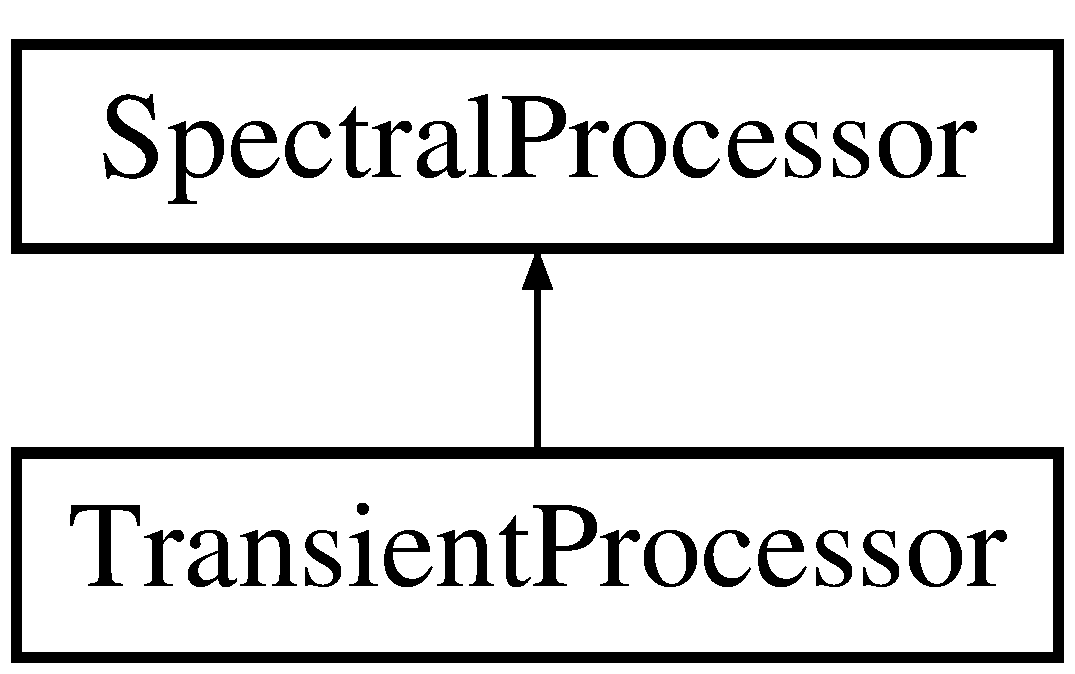
\includegraphics[height=2.000000cm]{class_spectral_processor}
\end{center}
\end{figure}
\subsection*{Public Member Functions}
\begin{DoxyCompactItemize}
\item 
virtual \hyperlink{class_spectral_processor_af63c533720981d19b64a1775b54b97f2}{$\sim$\+Spectral\+Processor} ()=0
\item 
virtual void \hyperlink{class_spectral_processor_a8e565ea203e58611f44f88c0dd2efecd}{process\+Transients} (\hyperlink{class_spectral_analyzer}{Spectral\+Analyzer} $\ast$analyzer, \hyperlink{_spectral_processor_8h_a7d90861a140b3b6cf1087c5662cf4223}{Analysis\+Type} t)=0
\end{DoxyCompactItemize}


\subsection{Constructor \& Destructor Documentation}
\hypertarget{class_spectral_processor_af63c533720981d19b64a1775b54b97f2}{\index{Spectral\+Processor@{Spectral\+Processor}!````~Spectral\+Processor@{$\sim$\+Spectral\+Processor}}
\index{````~Spectral\+Processor@{$\sim$\+Spectral\+Processor}!Spectral\+Processor@{Spectral\+Processor}}
\subsubsection[{$\sim$\+Spectral\+Processor}]{\setlength{\rightskip}{0pt plus 5cm}Spectral\+Processor\+::$\sim$\+Spectral\+Processor (
\begin{DoxyParamCaption}
{}
\end{DoxyParamCaption}
)\hspace{0.3cm}{\ttfamily [pure virtual]}}}\label{class_spectral_processor_af63c533720981d19b64a1775b54b97f2}


\subsection{Member Function Documentation}
\hypertarget{class_spectral_processor_a8e565ea203e58611f44f88c0dd2efecd}{\index{Spectral\+Processor@{Spectral\+Processor}!process\+Transients@{process\+Transients}}
\index{process\+Transients@{process\+Transients}!Spectral\+Processor@{Spectral\+Processor}}
\subsubsection[{process\+Transients}]{\setlength{\rightskip}{0pt plus 5cm}virtual void Spectral\+Processor\+::process\+Transients (
\begin{DoxyParamCaption}
\item[{{\bf Spectral\+Analyzer} $\ast$}]{analyzer, }
\item[{{\bf Analysis\+Type}}]{t}
\end{DoxyParamCaption}
)\hspace{0.3cm}{\ttfamily [pure virtual]}}}\label{class_spectral_processor_a8e565ea203e58611f44f88c0dd2efecd}


Implemented in \hyperlink{class_transient_processor_a66838cd9eb05f0e88360b2afce765dcf}{Transient\+Processor}.



The documentation for this class was generated from the following files\+:\begin{DoxyCompactItemize}
\item 
Analysis Classes/\+Headers/\hyperlink{_spectral_processor_8h}{Spectral\+Processor.\+h}\item 
Analysis Classes/\+Implementations/\hyperlink{_spectral_processor_8cpp}{Spectral\+Processor.\+cpp}\end{DoxyCompactItemize}

\hypertarget{class_transient_processor}{\section{Transient\+Processor Class Reference}
\label{class_transient_processor}\index{Transient\+Processor@{Transient\+Processor}}
}


{\ttfamily \#include $<$Transient\+Processor.\+h$>$}

Inheritance diagram for Transient\+Processor\+:\begin{figure}[H]
\begin{center}
\leavevmode
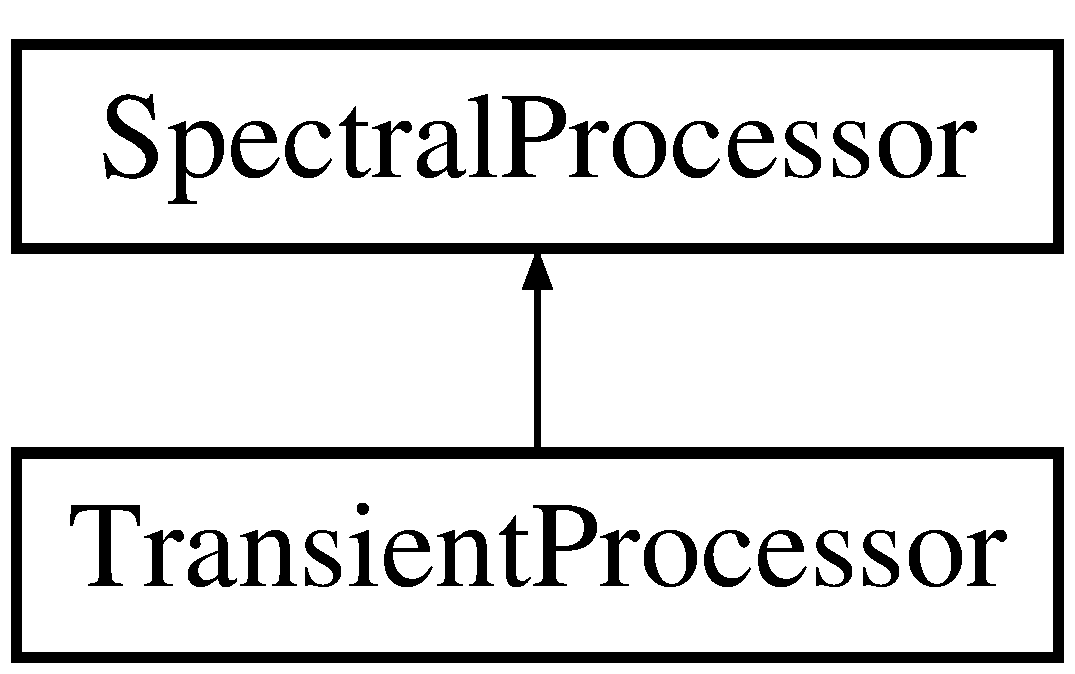
\includegraphics[height=2.000000cm]{class_transient_processor}
\end{center}
\end{figure}
\subsection*{Public Member Functions}
\begin{DoxyCompactItemize}
\item 
void \hyperlink{class_transient_processor_a66838cd9eb05f0e88360b2afce765dcf}{process\+Transients} (\hyperlink{class_spectral_analyzer}{Spectral\+Analyzer} $\ast$analyser, \hyperlink{_spectral_processor_8h_a7d90861a140b3b6cf1087c5662cf4223}{Analysis\+Type} t) override
\item 
std\+::vector$<$ float $>$ \hyperlink{class_transient_processor_ad51561a7e591bc06f669d19fcf5d02e7}{get\+Result} ()
\end{DoxyCompactItemize}


\subsection{Member Function Documentation}
\hypertarget{class_transient_processor_ad51561a7e591bc06f669d19fcf5d02e7}{\index{Transient\+Processor@{Transient\+Processor}!get\+Result@{get\+Result}}
\index{get\+Result@{get\+Result}!Transient\+Processor@{Transient\+Processor}}
\subsubsection[{get\+Result}]{\setlength{\rightskip}{0pt plus 5cm}std\+::vector$<$float$>$ Transient\+Processor\+::get\+Result (
\begin{DoxyParamCaption}
{}
\end{DoxyParamCaption}
)\hspace{0.3cm}{\ttfamily [inline]}}}\label{class_transient_processor_ad51561a7e591bc06f669d19fcf5d02e7}
\hypertarget{class_transient_processor_a66838cd9eb05f0e88360b2afce765dcf}{\index{Transient\+Processor@{Transient\+Processor}!process\+Transients@{process\+Transients}}
\index{process\+Transients@{process\+Transients}!Transient\+Processor@{Transient\+Processor}}
\subsubsection[{process\+Transients}]{\setlength{\rightskip}{0pt plus 5cm}void Transient\+Processor\+::process\+Transients (
\begin{DoxyParamCaption}
\item[{{\bf Spectral\+Analyzer} $\ast$}]{analyser, }
\item[{{\bf Analysis\+Type}}]{t}
\end{DoxyParamCaption}
)\hspace{0.3cm}{\ttfamily [override]}, {\ttfamily [virtual]}}}\label{class_transient_processor_a66838cd9eb05f0e88360b2afce765dcf}


Implements \hyperlink{class_spectral_processor_a8e565ea203e58611f44f88c0dd2efecd}{Spectral\+Processor}.



The documentation for this class was generated from the following files\+:\begin{DoxyCompactItemize}
\item 
Analysis Classes/\+Headers/\hyperlink{_transient_processor_8h}{Transient\+Processor.\+h}\item 
Analysis Classes/\+Implementations/\hyperlink{_transient_processor_8cpp}{Transient\+Processor.\+cpp}\end{DoxyCompactItemize}

\hypertarget{class_wave_form_component}{\section{Wave\+Form\+Component Class Reference}
\label{class_wave_form_component}\index{Wave\+Form\+Component@{Wave\+Form\+Component}}
}


{\ttfamily \#include $<$Wave\+Form\+Component.\+h$>$}

Inheritance diagram for Wave\+Form\+Component\+:\begin{figure}[H]
\begin{center}
\leavevmode
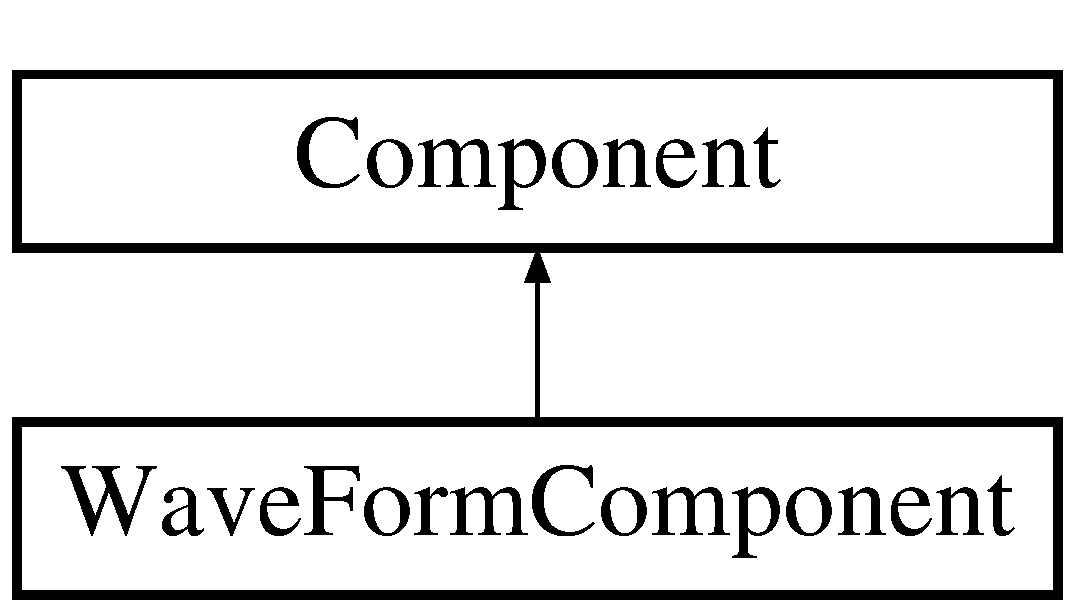
\includegraphics[height=2.000000cm]{class_wave_form_component}
\end{center}
\end{figure}
\subsection*{Public Member Functions}
\begin{DoxyCompactItemize}
\item 
\hyperlink{class_wave_form_component_a82a7cc74bc5355a0a287019b7306ecb2}{Wave\+Form\+Component} (\hyperlink{class_a_p_audio_file_manager}{A\+P\+Audio\+File\+Manager} $\ast$manager)
\item 
\hyperlink{class_wave_form_component_af8b2d3204b7e518e8738f974db60240e}{$\sim$\+Wave\+Form\+Component} ()
\item 
void \hyperlink{class_wave_form_component_aeb89cdc66b68aa25b33a61573a795a0c}{resized} () override
\item 
void \hyperlink{class_wave_form_component_a5f6f4f882beed2521df679ae576404ba}{paint} (Graphics \&g) override
\item 
void \hyperlink{class_wave_form_component_a13a99b881a8062850441e60f819181d0}{mouse\+Up} (const Mouse\+Event \&event) override
\item 
void \hyperlink{class_wave_form_component_affa835711f93fa3f10298befa5c9d9bc}{mouse\+Down} (const Mouse\+Event \&event) override
\item 
void \hyperlink{class_wave_form_component_a67bdb7a7900e21224684e154c123bcce}{load\+Data} (\hyperlink{class_a_p_audio_file}{A\+P\+Audio\+File} $\ast$file)
\item 
void \hyperlink{class_wave_form_component_af1878b5bf08aff80f1ef0d8220d97081}{fill\+Path} ()
\end{DoxyCompactItemize}


\subsection{Constructor \& Destructor Documentation}
\hypertarget{class_wave_form_component_a82a7cc74bc5355a0a287019b7306ecb2}{\index{Wave\+Form\+Component@{Wave\+Form\+Component}!Wave\+Form\+Component@{Wave\+Form\+Component}}
\index{Wave\+Form\+Component@{Wave\+Form\+Component}!Wave\+Form\+Component@{Wave\+Form\+Component}}
\subsubsection[{Wave\+Form\+Component}]{\setlength{\rightskip}{0pt plus 5cm}Wave\+Form\+Component\+::\+Wave\+Form\+Component (
\begin{DoxyParamCaption}
\item[{{\bf A\+P\+Audio\+File\+Manager} $\ast$}]{manager}
\end{DoxyParamCaption}
)}}\label{class_wave_form_component_a82a7cc74bc5355a0a287019b7306ecb2}
\hypertarget{class_wave_form_component_af8b2d3204b7e518e8738f974db60240e}{\index{Wave\+Form\+Component@{Wave\+Form\+Component}!````~Wave\+Form\+Component@{$\sim$\+Wave\+Form\+Component}}
\index{````~Wave\+Form\+Component@{$\sim$\+Wave\+Form\+Component}!Wave\+Form\+Component@{Wave\+Form\+Component}}
\subsubsection[{$\sim$\+Wave\+Form\+Component}]{\setlength{\rightskip}{0pt plus 5cm}Wave\+Form\+Component\+::$\sim$\+Wave\+Form\+Component (
\begin{DoxyParamCaption}
{}
\end{DoxyParamCaption}
)}}\label{class_wave_form_component_af8b2d3204b7e518e8738f974db60240e}


\subsection{Member Function Documentation}
\hypertarget{class_wave_form_component_af1878b5bf08aff80f1ef0d8220d97081}{\index{Wave\+Form\+Component@{Wave\+Form\+Component}!fill\+Path@{fill\+Path}}
\index{fill\+Path@{fill\+Path}!Wave\+Form\+Component@{Wave\+Form\+Component}}
\subsubsection[{fill\+Path}]{\setlength{\rightskip}{0pt plus 5cm}void Wave\+Form\+Component\+::fill\+Path (
\begin{DoxyParamCaption}
{}
\end{DoxyParamCaption}
)}}\label{class_wave_form_component_af1878b5bf08aff80f1ef0d8220d97081}
\hypertarget{class_wave_form_component_a67bdb7a7900e21224684e154c123bcce}{\index{Wave\+Form\+Component@{Wave\+Form\+Component}!load\+Data@{load\+Data}}
\index{load\+Data@{load\+Data}!Wave\+Form\+Component@{Wave\+Form\+Component}}
\subsubsection[{load\+Data}]{\setlength{\rightskip}{0pt plus 5cm}void Wave\+Form\+Component\+::load\+Data (
\begin{DoxyParamCaption}
\item[{{\bf A\+P\+Audio\+File} $\ast$}]{file}
\end{DoxyParamCaption}
)}}\label{class_wave_form_component_a67bdb7a7900e21224684e154c123bcce}
\hypertarget{class_wave_form_component_affa835711f93fa3f10298befa5c9d9bc}{\index{Wave\+Form\+Component@{Wave\+Form\+Component}!mouse\+Down@{mouse\+Down}}
\index{mouse\+Down@{mouse\+Down}!Wave\+Form\+Component@{Wave\+Form\+Component}}
\subsubsection[{mouse\+Down}]{\setlength{\rightskip}{0pt plus 5cm}void Wave\+Form\+Component\+::mouse\+Down (
\begin{DoxyParamCaption}
\item[{const Mouse\+Event \&}]{event}
\end{DoxyParamCaption}
)\hspace{0.3cm}{\ttfamily [override]}}}\label{class_wave_form_component_affa835711f93fa3f10298befa5c9d9bc}
\hypertarget{class_wave_form_component_a13a99b881a8062850441e60f819181d0}{\index{Wave\+Form\+Component@{Wave\+Form\+Component}!mouse\+Up@{mouse\+Up}}
\index{mouse\+Up@{mouse\+Up}!Wave\+Form\+Component@{Wave\+Form\+Component}}
\subsubsection[{mouse\+Up}]{\setlength{\rightskip}{0pt plus 5cm}void Wave\+Form\+Component\+::mouse\+Up (
\begin{DoxyParamCaption}
\item[{const Mouse\+Event \&}]{event}
\end{DoxyParamCaption}
)\hspace{0.3cm}{\ttfamily [override]}}}\label{class_wave_form_component_a13a99b881a8062850441e60f819181d0}
\hypertarget{class_wave_form_component_a5f6f4f882beed2521df679ae576404ba}{\index{Wave\+Form\+Component@{Wave\+Form\+Component}!paint@{paint}}
\index{paint@{paint}!Wave\+Form\+Component@{Wave\+Form\+Component}}
\subsubsection[{paint}]{\setlength{\rightskip}{0pt plus 5cm}void Wave\+Form\+Component\+::paint (
\begin{DoxyParamCaption}
\item[{Graphics \&}]{g}
\end{DoxyParamCaption}
)\hspace{0.3cm}{\ttfamily [override]}}}\label{class_wave_form_component_a5f6f4f882beed2521df679ae576404ba}
\hypertarget{class_wave_form_component_aeb89cdc66b68aa25b33a61573a795a0c}{\index{Wave\+Form\+Component@{Wave\+Form\+Component}!resized@{resized}}
\index{resized@{resized}!Wave\+Form\+Component@{Wave\+Form\+Component}}
\subsubsection[{resized}]{\setlength{\rightskip}{0pt plus 5cm}void Wave\+Form\+Component\+::resized (
\begin{DoxyParamCaption}
{}
\end{DoxyParamCaption}
)\hspace{0.3cm}{\ttfamily [override]}}}\label{class_wave_form_component_aeb89cdc66b68aa25b33a61573a795a0c}


The documentation for this class was generated from the following files\+:\begin{DoxyCompactItemize}
\item 
G\+U\+I Classes/\+Headers/\hyperlink{_wave_form_component_8h}{Wave\+Form\+Component.\+h}\item 
G\+U\+I Classes/\+Implementations/\hyperlink{_wave_form_component_8cpp}{Wave\+Form\+Component.\+cpp}\end{DoxyCompactItemize}

\hypertarget{class_wavelet_transform}{\section{Wavelet\+Transform Class Reference}
\label{class_wavelet_transform}\index{Wavelet\+Transform@{Wavelet\+Transform}}
}


{\ttfamily \#include $<$Wavelet\+Transform.\+h$>$}

\subsection*{Public Member Functions}
\begin{DoxyCompactItemize}
\item 
\hyperlink{class_wavelet_transform_a572cd14ad2377c0abf42b9992e485fee}{Wavelet\+Transform} ()
\item 
\hyperlink{class_wavelet_transform_ad334443b08026e7e78ed81f1ee269a1b}{$\sim$\+Wavelet\+Transform} ()
\item 
void \hyperlink{class_wavelet_transform_a95746d726b6e1a725e65116f18b59acb}{init} (int N)
\item 
void \hyperlink{class_wavelet_transform_a1f4688ce60f8ccc88919417451f21f44}{process} (float $\ast$input, int i)
\end{DoxyCompactItemize}


\subsection{Constructor \& Destructor Documentation}
\hypertarget{class_wavelet_transform_a572cd14ad2377c0abf42b9992e485fee}{\index{Wavelet\+Transform@{Wavelet\+Transform}!Wavelet\+Transform@{Wavelet\+Transform}}
\index{Wavelet\+Transform@{Wavelet\+Transform}!Wavelet\+Transform@{Wavelet\+Transform}}
\subsubsection[{Wavelet\+Transform}]{\setlength{\rightskip}{0pt plus 5cm}Wavelet\+Transform\+::\+Wavelet\+Transform (
\begin{DoxyParamCaption}
{}
\end{DoxyParamCaption}
)}}\label{class_wavelet_transform_a572cd14ad2377c0abf42b9992e485fee}
\hypertarget{class_wavelet_transform_ad334443b08026e7e78ed81f1ee269a1b}{\index{Wavelet\+Transform@{Wavelet\+Transform}!````~Wavelet\+Transform@{$\sim$\+Wavelet\+Transform}}
\index{````~Wavelet\+Transform@{$\sim$\+Wavelet\+Transform}!Wavelet\+Transform@{Wavelet\+Transform}}
\subsubsection[{$\sim$\+Wavelet\+Transform}]{\setlength{\rightskip}{0pt plus 5cm}Wavelet\+Transform\+::$\sim$\+Wavelet\+Transform (
\begin{DoxyParamCaption}
{}
\end{DoxyParamCaption}
)}}\label{class_wavelet_transform_ad334443b08026e7e78ed81f1ee269a1b}


\subsection{Member Function Documentation}
\hypertarget{class_wavelet_transform_a95746d726b6e1a725e65116f18b59acb}{\index{Wavelet\+Transform@{Wavelet\+Transform}!init@{init}}
\index{init@{init}!Wavelet\+Transform@{Wavelet\+Transform}}
\subsubsection[{init}]{\setlength{\rightskip}{0pt plus 5cm}void Wavelet\+Transform\+::init (
\begin{DoxyParamCaption}
\item[{int}]{N}
\end{DoxyParamCaption}
)}}\label{class_wavelet_transform_a95746d726b6e1a725e65116f18b59acb}
\hypertarget{class_wavelet_transform_a1f4688ce60f8ccc88919417451f21f44}{\index{Wavelet\+Transform@{Wavelet\+Transform}!process@{process}}
\index{process@{process}!Wavelet\+Transform@{Wavelet\+Transform}}
\subsubsection[{process}]{\setlength{\rightskip}{0pt plus 5cm}void Wavelet\+Transform\+::process (
\begin{DoxyParamCaption}
\item[{float $\ast$}]{input, }
\item[{int}]{i}
\end{DoxyParamCaption}
)}}\label{class_wavelet_transform_a1f4688ce60f8ccc88919417451f21f44}


The documentation for this class was generated from the following files\+:\begin{DoxyCompactItemize}
\item 
Analysis Classes/\+Headers/\hyperlink{_wavelet_transform_8h}{Wavelet\+Transform.\+h}\item 
Analysis Classes/\+Implementations/\hyperlink{_wavelet_transform_8cpp}{Wavelet\+Transform.\+cpp}\end{DoxyCompactItemize}

\hypertarget{class_y_i_n_analyzer}{\section{Y\+I\+N\+Analyzer Class Reference}
\label{class_y_i_n_analyzer}\index{Y\+I\+N\+Analyzer@{Y\+I\+N\+Analyzer}}
}


{\ttfamily \#include $<$Y\+I\+N\+Analyzer.\+h$>$}

\subsection*{Public Member Functions}
\begin{DoxyCompactItemize}
\item 
\hyperlink{class_y_i_n_analyzer_a2494dda10214a9c34a38b25896eaff7a}{Y\+I\+N\+Analyzer} ()
\item 
\hyperlink{class_y_i_n_analyzer_aa541be0da744d8b728a2319457463484}{$\sim$\+Y\+I\+N\+Analyzer} ()
\item 
void \hyperlink{class_y_i_n_analyzer_a663d8257e63802b77ad28ff6a429afe3}{init} (int N)
\item 
void \hyperlink{class_y_i_n_analyzer_a80223841c6c660bed5dd96d5b1ef9a01}{process} (float $\ast$audio\+Data, int num\+Samples)
\item 
float \hyperlink{class_y_i_n_analyzer_a5a4f6b977ef54b6e471ac240cedc2d10}{analyze} (float $\ast$input)
\end{DoxyCompactItemize}


\subsection{Constructor \& Destructor Documentation}
\hypertarget{class_y_i_n_analyzer_a2494dda10214a9c34a38b25896eaff7a}{\index{Y\+I\+N\+Analyzer@{Y\+I\+N\+Analyzer}!Y\+I\+N\+Analyzer@{Y\+I\+N\+Analyzer}}
\index{Y\+I\+N\+Analyzer@{Y\+I\+N\+Analyzer}!Y\+I\+N\+Analyzer@{Y\+I\+N\+Analyzer}}
\subsubsection[{Y\+I\+N\+Analyzer}]{\setlength{\rightskip}{0pt plus 5cm}Y\+I\+N\+Analyzer\+::\+Y\+I\+N\+Analyzer (
\begin{DoxyParamCaption}
{}
\end{DoxyParamCaption}
)}}\label{class_y_i_n_analyzer_a2494dda10214a9c34a38b25896eaff7a}
\hypertarget{class_y_i_n_analyzer_aa541be0da744d8b728a2319457463484}{\index{Y\+I\+N\+Analyzer@{Y\+I\+N\+Analyzer}!````~Y\+I\+N\+Analyzer@{$\sim$\+Y\+I\+N\+Analyzer}}
\index{````~Y\+I\+N\+Analyzer@{$\sim$\+Y\+I\+N\+Analyzer}!Y\+I\+N\+Analyzer@{Y\+I\+N\+Analyzer}}
\subsubsection[{$\sim$\+Y\+I\+N\+Analyzer}]{\setlength{\rightskip}{0pt plus 5cm}Y\+I\+N\+Analyzer\+::$\sim$\+Y\+I\+N\+Analyzer (
\begin{DoxyParamCaption}
{}
\end{DoxyParamCaption}
)}}\label{class_y_i_n_analyzer_aa541be0da744d8b728a2319457463484}


\subsection{Member Function Documentation}
\hypertarget{class_y_i_n_analyzer_a5a4f6b977ef54b6e471ac240cedc2d10}{\index{Y\+I\+N\+Analyzer@{Y\+I\+N\+Analyzer}!analyze@{analyze}}
\index{analyze@{analyze}!Y\+I\+N\+Analyzer@{Y\+I\+N\+Analyzer}}
\subsubsection[{analyze}]{\setlength{\rightskip}{0pt plus 5cm}float Y\+I\+N\+Analyzer\+::analyze (
\begin{DoxyParamCaption}
\item[{float $\ast$}]{input}
\end{DoxyParamCaption}
)}}\label{class_y_i_n_analyzer_a5a4f6b977ef54b6e471ac240cedc2d10}
\hypertarget{class_y_i_n_analyzer_a663d8257e63802b77ad28ff6a429afe3}{\index{Y\+I\+N\+Analyzer@{Y\+I\+N\+Analyzer}!init@{init}}
\index{init@{init}!Y\+I\+N\+Analyzer@{Y\+I\+N\+Analyzer}}
\subsubsection[{init}]{\setlength{\rightskip}{0pt plus 5cm}void Y\+I\+N\+Analyzer\+::init (
\begin{DoxyParamCaption}
\item[{int}]{N}
\end{DoxyParamCaption}
)}}\label{class_y_i_n_analyzer_a663d8257e63802b77ad28ff6a429afe3}
\hypertarget{class_y_i_n_analyzer_a80223841c6c660bed5dd96d5b1ef9a01}{\index{Y\+I\+N\+Analyzer@{Y\+I\+N\+Analyzer}!process@{process}}
\index{process@{process}!Y\+I\+N\+Analyzer@{Y\+I\+N\+Analyzer}}
\subsubsection[{process}]{\setlength{\rightskip}{0pt plus 5cm}void Y\+I\+N\+Analyzer\+::process (
\begin{DoxyParamCaption}
\item[{float $\ast$}]{audio\+Data, }
\item[{int}]{num\+Samples}
\end{DoxyParamCaption}
)}}\label{class_y_i_n_analyzer_a80223841c6c660bed5dd96d5b1ef9a01}


The documentation for this class was generated from the following files\+:\begin{DoxyCompactItemize}
\item 
Analysis Classes/\+Headers/\hyperlink{_y_i_n_analyzer_8h}{Y\+I\+N\+Analyzer.\+h}\item 
Analysis Classes/\+Implementations/\hyperlink{_y_i_n_analyzer_8cpp}{Y\+I\+N\+Analyzer.\+cpp}\end{DoxyCompactItemize}

\hypertarget{class_y_i_n_pitch_graph}{\section{Y\+I\+N\+Pitch\+Graph Class Reference}
\label{class_y_i_n_pitch_graph}\index{Y\+I\+N\+Pitch\+Graph@{Y\+I\+N\+Pitch\+Graph}}
}


{\ttfamily \#include $<$Y\+I\+N\+Pitch\+Graph.\+h$>$}

Inheritance diagram for Y\+I\+N\+Pitch\+Graph\+:\begin{figure}[H]
\begin{center}
\leavevmode
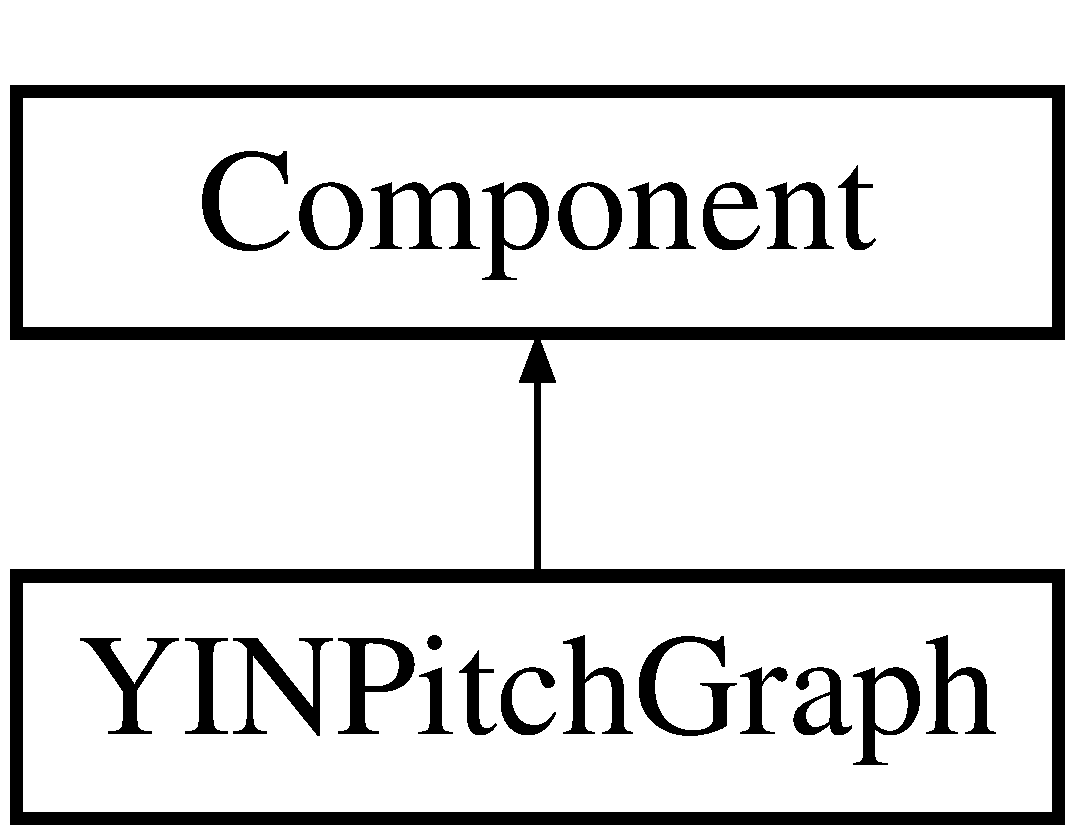
\includegraphics[height=2.000000cm]{class_y_i_n_pitch_graph}
\end{center}
\end{figure}
\subsection*{Public Member Functions}
\begin{DoxyCompactItemize}
\item 
\hyperlink{class_y_i_n_pitch_graph_a7d4889a077f978a552c98f4961367db7}{Y\+I\+N\+Pitch\+Graph} (\hyperlink{class_a_p_audio_file_manager}{A\+P\+Audio\+File\+Manager} $\ast$file\+Manager, \hyperlink{class_y_i_n_analyzer}{Y\+I\+N\+Analyzer} $\ast$analyzer)
\item 
\hyperlink{class_y_i_n_pitch_graph_a55d8c0a35265cc9adbf4cd3ee909ba51}{Y\+I\+N\+Pitch\+Graph} ()
\item 
void \hyperlink{class_y_i_n_pitch_graph_a0fcd725ef86ecbd35c498cc98dd91c4f}{resized} () overridefinal
\item 
void \hyperlink{class_y_i_n_pitch_graph_a7388ed6a8b4c3b579a73c78e0effdb59}{paint} (Graphics \&g) overridefinal
\end{DoxyCompactItemize}


\subsection{Constructor \& Destructor Documentation}
\hypertarget{class_y_i_n_pitch_graph_a7d4889a077f978a552c98f4961367db7}{\index{Y\+I\+N\+Pitch\+Graph@{Y\+I\+N\+Pitch\+Graph}!Y\+I\+N\+Pitch\+Graph@{Y\+I\+N\+Pitch\+Graph}}
\index{Y\+I\+N\+Pitch\+Graph@{Y\+I\+N\+Pitch\+Graph}!Y\+I\+N\+Pitch\+Graph@{Y\+I\+N\+Pitch\+Graph}}
\subsubsection[{Y\+I\+N\+Pitch\+Graph}]{\setlength{\rightskip}{0pt plus 5cm}Y\+I\+N\+Pitch\+Graph\+::\+Y\+I\+N\+Pitch\+Graph (
\begin{DoxyParamCaption}
\item[{{\bf A\+P\+Audio\+File\+Manager} $\ast$}]{file\+Manager, }
\item[{{\bf Y\+I\+N\+Analyzer} $\ast$}]{analyzer}
\end{DoxyParamCaption}
)}}\label{class_y_i_n_pitch_graph_a7d4889a077f978a552c98f4961367db7}
\hypertarget{class_y_i_n_pitch_graph_a55d8c0a35265cc9adbf4cd3ee909ba51}{\index{Y\+I\+N\+Pitch\+Graph@{Y\+I\+N\+Pitch\+Graph}!Y\+I\+N\+Pitch\+Graph@{Y\+I\+N\+Pitch\+Graph}}
\index{Y\+I\+N\+Pitch\+Graph@{Y\+I\+N\+Pitch\+Graph}!Y\+I\+N\+Pitch\+Graph@{Y\+I\+N\+Pitch\+Graph}}
\subsubsection[{Y\+I\+N\+Pitch\+Graph}]{\setlength{\rightskip}{0pt plus 5cm}Y\+I\+N\+Pitch\+Graph\+::\+Y\+I\+N\+Pitch\+Graph (
\begin{DoxyParamCaption}
{}
\end{DoxyParamCaption}
)}}\label{class_y_i_n_pitch_graph_a55d8c0a35265cc9adbf4cd3ee909ba51}


\subsection{Member Function Documentation}
\hypertarget{class_y_i_n_pitch_graph_a7388ed6a8b4c3b579a73c78e0effdb59}{\index{Y\+I\+N\+Pitch\+Graph@{Y\+I\+N\+Pitch\+Graph}!paint@{paint}}
\index{paint@{paint}!Y\+I\+N\+Pitch\+Graph@{Y\+I\+N\+Pitch\+Graph}}
\subsubsection[{paint}]{\setlength{\rightskip}{0pt plus 5cm}void Y\+I\+N\+Pitch\+Graph\+::paint (
\begin{DoxyParamCaption}
\item[{Graphics \&}]{g}
\end{DoxyParamCaption}
)\hspace{0.3cm}{\ttfamily [final]}, {\ttfamily [override]}}}\label{class_y_i_n_pitch_graph_a7388ed6a8b4c3b579a73c78e0effdb59}
\hypertarget{class_y_i_n_pitch_graph_a0fcd725ef86ecbd35c498cc98dd91c4f}{\index{Y\+I\+N\+Pitch\+Graph@{Y\+I\+N\+Pitch\+Graph}!resized@{resized}}
\index{resized@{resized}!Y\+I\+N\+Pitch\+Graph@{Y\+I\+N\+Pitch\+Graph}}
\subsubsection[{resized}]{\setlength{\rightskip}{0pt plus 5cm}void Y\+I\+N\+Pitch\+Graph\+::resized (
\begin{DoxyParamCaption}
{}
\end{DoxyParamCaption}
)\hspace{0.3cm}{\ttfamily [final]}, {\ttfamily [override]}}}\label{class_y_i_n_pitch_graph_a0fcd725ef86ecbd35c498cc98dd91c4f}


The documentation for this class was generated from the following file\+:\begin{DoxyCompactItemize}
\item 
G\+U\+I Classes/\hyperlink{_y_i_n_pitch_graph_8h}{Y\+I\+N\+Pitch\+Graph.\+h}\end{DoxyCompactItemize}

\chapter{File Documentation}
\hypertarget{_d_f_t_8h}{\section{Analysis Classes/\+Headers/\+D\+F\+T.h File Reference}
\label{_d_f_t_8h}\index{Analysis Classes/\+Headers/\+D\+F\+T.\+h@{Analysis Classes/\+Headers/\+D\+F\+T.\+h}}
}
{\ttfamily \#include $<$vector$>$}\\*
{\ttfamily \#include $<$complex$>$}\\*
{\ttfamily \#include \char`\"{}Utility.\+h\char`\"{}}\\*
\subsection*{Classes}
\begin{DoxyCompactItemize}
\item 
class \hyperlink{class_d_f_t}{D\+F\+T}
\end{DoxyCompactItemize}

\hypertarget{_d_f_t_analyzer_8h}{\section{Analysis Classes/\+Headers/\+D\+F\+T\+Analyzer.h File Reference}
\label{_d_f_t_analyzer_8h}\index{Analysis Classes/\+Headers/\+D\+F\+T\+Analyzer.\+h@{Analysis Classes/\+Headers/\+D\+F\+T\+Analyzer.\+h}}
}
{\ttfamily \#include \char`\"{}Spectral\+Analyzer.\+h\char`\"{}}\\*
{\ttfamily \#include \char`\"{}D\+F\+T.\+h\char`\"{}}\\*
\subsection*{Classes}
\begin{DoxyCompactItemize}
\item 
class \hyperlink{class_d_f_t_analyzer}{D\+F\+T\+Analyzer}
\end{DoxyCompactItemize}

\hypertarget{_fast_wavelet_8h}{\section{Analysis Classes/\+Headers/\+Fast\+Wavelet.h File Reference}
\label{_fast_wavelet_8h}\index{Analysis Classes/\+Headers/\+Fast\+Wavelet.\+h@{Analysis Classes/\+Headers/\+Fast\+Wavelet.\+h}}
}
{\ttfamily \#include $<$math.\+h$>$}\\*
{\ttfamily \#include $<$vector$>$}\\*
\subsection*{Classes}
\begin{DoxyCompactItemize}
\item 
class \hyperlink{class_fast_wavelet}{Fast\+Wavelet}
\end{DoxyCompactItemize}

\hypertarget{_fast_wavelet_analyzer_8h}{\section{Analysis Classes/\+Headers/\+Fast\+Wavelet\+Analyzer.h File Reference}
\label{_fast_wavelet_analyzer_8h}\index{Analysis Classes/\+Headers/\+Fast\+Wavelet\+Analyzer.\+h@{Analysis Classes/\+Headers/\+Fast\+Wavelet\+Analyzer.\+h}}
}
{\ttfamily \#include \char`\"{}Fast\+Wavelet.\+h\char`\"{}}\\*
{\ttfamily \#include \char`\"{}Spectral\+Analyzer.\+h\char`\"{}}\\*
\subsection*{Classes}
\begin{DoxyCompactItemize}
\item 
class \hyperlink{class_fast_wavelet_analyzer}{Fast\+Wavelet\+Analyzer}
\end{DoxyCompactItemize}

\hypertarget{_frequency_analyzer_8h}{\section{Analysis Classes/\+Headers/\+Frequency\+Analyzer.h File Reference}
\label{_frequency_analyzer_8h}\index{Analysis Classes/\+Headers/\+Frequency\+Analyzer.\+h@{Analysis Classes/\+Headers/\+Frequency\+Analyzer.\+h}}
}
{\ttfamily \#include \char`\"{}Y\+I\+N\+Analyzer.\+h\char`\"{}}\\*
{\ttfamily \#include \char`\"{}A\+P\+Audio\+File\+Manager2.\+h\char`\"{}}\\*
\subsection*{Classes}
\begin{DoxyCompactItemize}
\item 
class \hyperlink{class_frequency_analyzer}{Frequency\+Analyzer}
\end{DoxyCompactItemize}

\hypertarget{_multi_resolution_transform_8h}{\section{Analysis Classes/\+Headers/\+Multi\+Resolution\+Transform.h File Reference}
\label{_multi_resolution_transform_8h}\index{Analysis Classes/\+Headers/\+Multi\+Resolution\+Transform.\+h@{Analysis Classes/\+Headers/\+Multi\+Resolution\+Transform.\+h}}
}
{\ttfamily \#include \char`\"{}Wavelet\+Transform.\+h\char`\"{}}\\*
{\ttfamily \#include \char`\"{}Spectral\+Analyzer.\+h\char`\"{}}\\*
\subsection*{Classes}
\begin{DoxyCompactItemize}
\item 
class \hyperlink{class_multi_resolution_transform}{Multi\+Resolution\+Transform}
\end{DoxyCompactItemize}

\hypertarget{_spectral_analyzer_8h}{\section{Analysis Classes/\+Headers/\+Spectral\+Analyzer.h File Reference}
\label{_spectral_analyzer_8h}\index{Analysis Classes/\+Headers/\+Spectral\+Analyzer.\+h@{Analysis Classes/\+Headers/\+Spectral\+Analyzer.\+h}}
}
{\ttfamily \#include $<$math.\+h$>$}\\*
\subsection*{Classes}
\begin{DoxyCompactItemize}
\item 
class \hyperlink{class_spectral_analyzer}{Spectral\+Analyzer}
\end{DoxyCompactItemize}

\hypertarget{_spectral_processor_8h}{\section{Analysis Classes/\+Headers/\+Spectral\+Processor.h File Reference}
\label{_spectral_processor_8h}\index{Analysis Classes/\+Headers/\+Spectral\+Processor.\+h@{Analysis Classes/\+Headers/\+Spectral\+Processor.\+h}}
}
{\ttfamily \#include \char`\"{}Spectral\+Analyzer.\+h\char`\"{}}\\*
{\ttfamily \#include $<$vector$>$}\\*
\subsection*{Classes}
\begin{DoxyCompactItemize}
\item 
class \hyperlink{class_spectral_processor}{Spectral\+Processor}
\end{DoxyCompactItemize}
\subsection*{Enumerations}
\begin{DoxyCompactItemize}
\item 
enum \hyperlink{_spectral_processor_8h_a7d90861a140b3b6cf1087c5662cf4223}{Analysis\+Type} \{ \hyperlink{_spectral_processor_8h_a7d90861a140b3b6cf1087c5662cf4223ac97a499554efa6ba8803085f3dd04888}{D\+F\+T}
 \}
\end{DoxyCompactItemize}


\subsection{Enumeration Type Documentation}
\hypertarget{_spectral_processor_8h_a7d90861a140b3b6cf1087c5662cf4223}{\index{Spectral\+Processor.\+h@{Spectral\+Processor.\+h}!Analysis\+Type@{Analysis\+Type}}
\index{Analysis\+Type@{Analysis\+Type}!Spectral\+Processor.\+h@{Spectral\+Processor.\+h}}
\subsubsection[{Analysis\+Type}]{\setlength{\rightskip}{0pt plus 5cm}enum {\bf Analysis\+Type}}}\label{_spectral_processor_8h_a7d90861a140b3b6cf1087c5662cf4223}
\begin{Desc}
\item[Enumerator]\par
\begin{description}
\index{D\+F\+T@{D\+F\+T}!Spectral\+Processor.\+h@{Spectral\+Processor.\+h}}\index{Spectral\+Processor.\+h@{Spectral\+Processor.\+h}!D\+F\+T@{D\+F\+T}}\item[{\em 
\hypertarget{_spectral_processor_8h_a7d90861a140b3b6cf1087c5662cf4223ac97a499554efa6ba8803085f3dd04888}{D\+F\+T}\label{_spectral_processor_8h_a7d90861a140b3b6cf1087c5662cf4223ac97a499554efa6ba8803085f3dd04888}
}]\end{description}
\end{Desc}

\hypertarget{_transient_processor_8h}{\section{Analysis Classes/\+Headers/\+Transient\+Processor.h File Reference}
\label{_transient_processor_8h}\index{Analysis Classes/\+Headers/\+Transient\+Processor.\+h@{Analysis Classes/\+Headers/\+Transient\+Processor.\+h}}
}
{\ttfamily \#include \char`\"{}Spectral\+Processor.\+h\char`\"{}}\\*
{\ttfamily \#include \char`\"{}D\+F\+T\+Analyzer.\+h\char`\"{}}\\*
{\ttfamily \#include $<$iostream$>$}\\*
\subsection*{Classes}
\begin{DoxyCompactItemize}
\item 
class \hyperlink{class_transient_processor}{Transient\+Processor}
\end{DoxyCompactItemize}

\hypertarget{_wavelet_transform_8h}{\section{Analysis Classes/\+Headers/\+Wavelet\+Transform.h File Reference}
\label{_wavelet_transform_8h}\index{Analysis Classes/\+Headers/\+Wavelet\+Transform.\+h@{Analysis Classes/\+Headers/\+Wavelet\+Transform.\+h}}
}
{\ttfamily \#include \char`\"{}Utility.\+h\char`\"{}}\\*
{\ttfamily \#include $<$complex$>$}\\*
{\ttfamily \#include $<$vector$>$}\\*
{\ttfamily \#include $<$iostream$>$}\\*
\subsection*{Classes}
\begin{DoxyCompactItemize}
\item 
class \hyperlink{class_wavelet_transform}{Wavelet\+Transform}
\end{DoxyCompactItemize}

\hypertarget{_y_i_n_analyzer_8h}{\section{Analysis Classes/\+Headers/\+Y\+I\+N\+Analyzer.h File Reference}
\label{_y_i_n_analyzer_8h}\index{Analysis Classes/\+Headers/\+Y\+I\+N\+Analyzer.\+h@{Analysis Classes/\+Headers/\+Y\+I\+N\+Analyzer.\+h}}
}
{\ttfamily \#include $<$vector$>$}\\*
{\ttfamily \#include \char`\"{}Utility.\+h\char`\"{}}\\*
{\ttfamily \#include $<$iostream$>$}\\*
\subsection*{Classes}
\begin{DoxyCompactItemize}
\item 
class \hyperlink{class_y_i_n_analyzer}{Y\+I\+N\+Analyzer}
\end{DoxyCompactItemize}

\hypertarget{_d_f_t_8cpp}{\section{Analysis Classes/\+Implementations/\+D\+F\+T.cpp File Reference}
\label{_d_f_t_8cpp}\index{Analysis Classes/\+Implementations/\+D\+F\+T.\+cpp@{Analysis Classes/\+Implementations/\+D\+F\+T.\+cpp}}
}
{\ttfamily \#include \char`\"{}D\+F\+T.\+h\char`\"{}}\\*

\hypertarget{_d_f_t_analyzer_8cpp}{\section{Analysis Classes/\+Implementations/\+D\+F\+T\+Analyzer.cpp File Reference}
\label{_d_f_t_analyzer_8cpp}\index{Analysis Classes/\+Implementations/\+D\+F\+T\+Analyzer.\+cpp@{Analysis Classes/\+Implementations/\+D\+F\+T\+Analyzer.\+cpp}}
}
{\ttfamily \#include \char`\"{}D\+F\+T\+Analyzer.\+h\char`\"{}}\\*
{\ttfamily \#include \char`\"{}Y\+I\+N\+Analyzer.\+h\char`\"{}}\\*

\hypertarget{_fast_wavelet_8cpp}{\section{Analysis Classes/\+Implementations/\+Fast\+Wavelet.cpp File Reference}
\label{_fast_wavelet_8cpp}\index{Analysis Classes/\+Implementations/\+Fast\+Wavelet.\+cpp@{Analysis Classes/\+Implementations/\+Fast\+Wavelet.\+cpp}}
}
{\ttfamily \#include \char`\"{}Fast\+Wavelet.\+h\char`\"{}}\\*

\hypertarget{_fast_wavelet_analyzer_8cpp}{\section{Analysis Classes/\+Implementations/\+Fast\+Wavelet\+Analyzer.cpp File Reference}
\label{_fast_wavelet_analyzer_8cpp}\index{Analysis Classes/\+Implementations/\+Fast\+Wavelet\+Analyzer.\+cpp@{Analysis Classes/\+Implementations/\+Fast\+Wavelet\+Analyzer.\+cpp}}
}
{\ttfamily \#include \char`\"{}Fast\+Wavelet\+Analyzer.\+h\char`\"{}}\\*

\hypertarget{_frequency_analyzer_8cpp}{\section{Analysis Classes/\+Implementations/\+Frequency\+Analyzer.cpp File Reference}
\label{_frequency_analyzer_8cpp}\index{Analysis Classes/\+Implementations/\+Frequency\+Analyzer.\+cpp@{Analysis Classes/\+Implementations/\+Frequency\+Analyzer.\+cpp}}
}
{\ttfamily \#include \char`\"{}Frequency\+Analyzer.\+h\char`\"{}}\\*

\hypertarget{_multi_resolution_transform_8cpp}{\section{Analysis Classes/\+Implementations/\+Multi\+Resolution\+Transform.cpp File Reference}
\label{_multi_resolution_transform_8cpp}\index{Analysis Classes/\+Implementations/\+Multi\+Resolution\+Transform.\+cpp@{Analysis Classes/\+Implementations/\+Multi\+Resolution\+Transform.\+cpp}}
}
{\ttfamily \#include \char`\"{}Multi\+Resolution\+Transform.\+h\char`\"{}}\\*

\hypertarget{_spectral_analyzer_8cpp}{\section{Analysis Classes/\+Implementations/\+Spectral\+Analyzer.cpp File Reference}
\label{_spectral_analyzer_8cpp}\index{Analysis Classes/\+Implementations/\+Spectral\+Analyzer.\+cpp@{Analysis Classes/\+Implementations/\+Spectral\+Analyzer.\+cpp}}
}
{\ttfamily \#include \char`\"{}Spectral\+Analyzer.\+h\char`\"{}}\\*

\hypertarget{_spectral_processor_8cpp}{\section{Analysis Classes/\+Implementations/\+Spectral\+Processor.cpp File Reference}
\label{_spectral_processor_8cpp}\index{Analysis Classes/\+Implementations/\+Spectral\+Processor.\+cpp@{Analysis Classes/\+Implementations/\+Spectral\+Processor.\+cpp}}
}
{\ttfamily \#include \char`\"{}Spectral\+Processor.\+h\char`\"{}}\\*

\hypertarget{_transient_processor_8cpp}{\section{Analysis Classes/\+Implementations/\+Transient\+Processor.cpp File Reference}
\label{_transient_processor_8cpp}\index{Analysis Classes/\+Implementations/\+Transient\+Processor.\+cpp@{Analysis Classes/\+Implementations/\+Transient\+Processor.\+cpp}}
}
{\ttfamily \#include \char`\"{}Transient\+Processor.\+h\char`\"{}}\\*

\hypertarget{_utility_8h}{\section{Analysis Classes/\+Implementations/\+Utility.h File Reference}
\label{_utility_8h}\index{Analysis Classes/\+Implementations/\+Utility.\+h@{Analysis Classes/\+Implementations/\+Utility.\+h}}
}
{\ttfamily \#include $<$math.\+h$>$}\\*
{\ttfamily \#include $<$algorithm$>$}\\*
\subsection*{Enumerations}
\begin{DoxyCompactItemize}
\item 
enum \hyperlink{_utility_8h_a476342970f954b62d70552bcbb5ee509}{Window\+Type} \{ \hyperlink{_utility_8h_a476342970f954b62d70552bcbb5ee509a1a1594aa252fb4958a0f79394592129d}{H\+A\+N\+N\+I\+N\+G}, 
\hyperlink{_utility_8h_a476342970f954b62d70552bcbb5ee509ace0d8d5669106f95e034b2ad3bc8659b}{H\+A\+M\+M\+I\+N\+G}, 
\hyperlink{_utility_8h_a476342970f954b62d70552bcbb5ee509a32200a8a5676be63f32a24e70f3ce1bc}{B\+L\+A\+C\+K\+M\+A\+N}
 \}
\end{DoxyCompactItemize}


\subsection{Enumeration Type Documentation}
\hypertarget{_utility_8h_a476342970f954b62d70552bcbb5ee509}{\index{Utility.\+h@{Utility.\+h}!Window\+Type@{Window\+Type}}
\index{Window\+Type@{Window\+Type}!Utility.\+h@{Utility.\+h}}
\subsubsection[{Window\+Type}]{\setlength{\rightskip}{0pt plus 5cm}enum {\bf Window\+Type}}}\label{_utility_8h_a476342970f954b62d70552bcbb5ee509}
\begin{Desc}
\item[Enumerator]\par
\begin{description}
\index{H\+A\+N\+N\+I\+N\+G@{H\+A\+N\+N\+I\+N\+G}!Utility.\+h@{Utility.\+h}}\index{Utility.\+h@{Utility.\+h}!H\+A\+N\+N\+I\+N\+G@{H\+A\+N\+N\+I\+N\+G}}\item[{\em 
\hypertarget{_utility_8h_a476342970f954b62d70552bcbb5ee509a1a1594aa252fb4958a0f79394592129d}{H\+A\+N\+N\+I\+N\+G}\label{_utility_8h_a476342970f954b62d70552bcbb5ee509a1a1594aa252fb4958a0f79394592129d}
}]\index{H\+A\+M\+M\+I\+N\+G@{H\+A\+M\+M\+I\+N\+G}!Utility.\+h@{Utility.\+h}}\index{Utility.\+h@{Utility.\+h}!H\+A\+M\+M\+I\+N\+G@{H\+A\+M\+M\+I\+N\+G}}\item[{\em 
\hypertarget{_utility_8h_a476342970f954b62d70552bcbb5ee509ace0d8d5669106f95e034b2ad3bc8659b}{H\+A\+M\+M\+I\+N\+G}\label{_utility_8h_a476342970f954b62d70552bcbb5ee509ace0d8d5669106f95e034b2ad3bc8659b}
}]\index{B\+L\+A\+C\+K\+M\+A\+N@{B\+L\+A\+C\+K\+M\+A\+N}!Utility.\+h@{Utility.\+h}}\index{Utility.\+h@{Utility.\+h}!B\+L\+A\+C\+K\+M\+A\+N@{B\+L\+A\+C\+K\+M\+A\+N}}\item[{\em 
\hypertarget{_utility_8h_a476342970f954b62d70552bcbb5ee509a32200a8a5676be63f32a24e70f3ce1bc}{B\+L\+A\+C\+K\+M\+A\+N}\label{_utility_8h_a476342970f954b62d70552bcbb5ee509a32200a8a5676be63f32a24e70f3ce1bc}
}]\end{description}
\end{Desc}

\hypertarget{_wavelet_transform_8cpp}{\section{Analysis Classes/\+Implementations/\+Wavelet\+Transform.cpp File Reference}
\label{_wavelet_transform_8cpp}\index{Analysis Classes/\+Implementations/\+Wavelet\+Transform.\+cpp@{Analysis Classes/\+Implementations/\+Wavelet\+Transform.\+cpp}}
}
{\ttfamily \#include \char`\"{}Wavelet\+Transform.\+h\char`\"{}}\\*

\hypertarget{_y_i_n_analyzer_8cpp}{\section{Analysis Classes/\+Implementations/\+Y\+I\+N\+Analyzer.cpp File Reference}
\label{_y_i_n_analyzer_8cpp}\index{Analysis Classes/\+Implementations/\+Y\+I\+N\+Analyzer.\+cpp@{Analysis Classes/\+Implementations/\+Y\+I\+N\+Analyzer.\+cpp}}
}
{\ttfamily \#include \char`\"{}Y\+I\+N\+Analyzer.\+h\char`\"{}}\\*

\hypertarget{_a_p_audio_decimator_module_8h}{\section{Audio Classes/\+Headers/\+A\+P\+Audio\+Decimator\+Module.h File Reference}
\label{_a_p_audio_decimator_module_8h}\index{Audio Classes/\+Headers/\+A\+P\+Audio\+Decimator\+Module.\+h@{Audio Classes/\+Headers/\+A\+P\+Audio\+Decimator\+Module.\+h}}
}
{\ttfamily \#include \char`\"{}A\+P\+Audio\+Module.\+h\char`\"{}}\\*
\subsection*{Classes}
\begin{DoxyCompactItemize}
\item 
class \hyperlink{class_a_p_audio_decimator_module}{A\+P\+Audio\+Decimator\+Module}
\end{DoxyCompactItemize}

\hypertarget{_a_p_audio_envelope_8h}{\section{Audio Classes/\+Headers/\+A\+P\+Audio\+Envelope.h File Reference}
\label{_a_p_audio_envelope_8h}\index{Audio Classes/\+Headers/\+A\+P\+Audio\+Envelope.\+h@{Audio Classes/\+Headers/\+A\+P\+Audio\+Envelope.\+h}}
}
{\ttfamily \#include \char`\"{}A\+P\+Audio\+Module.\+h\char`\"{}}\\*
\subsection*{Classes}
\begin{DoxyCompactItemize}
\item 
class \hyperlink{class_a_p_audio_envelope}{A\+P\+Audio\+Envelope}
\end{DoxyCompactItemize}

\hypertarget{_a_p_audio_file_8h}{\section{Audio Classes/\+Headers/\+A\+P\+Audio\+File.h File Reference}
\label{_a_p_audio_file_8h}\index{Audio Classes/\+Headers/\+A\+P\+Audio\+File.\+h@{Audio Classes/\+Headers/\+A\+P\+Audio\+File.\+h}}
}
{\ttfamily \#include \char`\"{}../\+Juce\+Library\+Code/\+Juce\+Header.\+h\char`\"{}}\\*
\subsection*{Classes}
\begin{DoxyCompactItemize}
\item 
class \hyperlink{class_a_p_audio_file}{A\+P\+Audio\+File}
\end{DoxyCompactItemize}

\hypertarget{_a_p_audio_file_manager2_8h}{\section{Audio Classes/\+Headers/\+A\+P\+Audio\+File\+Manager2.h File Reference}
\label{_a_p_audio_file_manager2_8h}\index{Audio Classes/\+Headers/\+A\+P\+Audio\+File\+Manager2.\+h@{Audio Classes/\+Headers/\+A\+P\+Audio\+File\+Manager2.\+h}}
}
{\ttfamily \#include \char`\"{}A\+P\+Audio\+File.\+h\char`\"{}}\\*
{\ttfamily \#include $<$vector$>$}\\*
{\ttfamily \#include $<$memory$>$}\\*
\subsection*{Classes}
\begin{DoxyCompactItemize}
\item 
class \hyperlink{class_a_p_audio_file_manager}{A\+P\+Audio\+File\+Manager}
\end{DoxyCompactItemize}

\hypertarget{_a_p_audio_file_player_8h}{\section{Audio Classes/\+Headers/\+A\+P\+Audio\+File\+Player.h File Reference}
\label{_a_p_audio_file_player_8h}\index{Audio Classes/\+Headers/\+A\+P\+Audio\+File\+Player.\+h@{Audio Classes/\+Headers/\+A\+P\+Audio\+File\+Player.\+h}}
}
{\ttfamily \#include \char`\"{}A\+P\+Audio\+File.\+h\char`\"{}}\\*
\subsection*{Classes}
\begin{DoxyCompactItemize}
\item 
class \hyperlink{class_a_p_audio_file_player}{A\+P\+Audio\+File\+Player}
\end{DoxyCompactItemize}

\hypertarget{_a_p_audio_module_8h}{\section{Audio Classes/\+Headers/\+A\+P\+Audio\+Module.h File Reference}
\label{_a_p_audio_module_8h}\index{Audio Classes/\+Headers/\+A\+P\+Audio\+Module.\+h@{Audio Classes/\+Headers/\+A\+P\+Audio\+Module.\+h}}
}
{\ttfamily \#include $<$vector$>$}\\*
{\ttfamily \#include $<$stdlib.\+h$>$}\\*
{\ttfamily \#include $<$string$>$}\\*
{\ttfamily \#include $<$iostream$>$}\\*
{\ttfamily \#include \char`\"{}../\+Juce\+Library\+Code/\+Juce\+Header.\+h\char`\"{}}\\*
\subsection*{Classes}
\begin{DoxyCompactItemize}
\item 
class \hyperlink{class_a_p_audio_main_frame}{A\+P\+Audio\+Main\+Frame}
\item 
class \hyperlink{class_a_p_audio_module}{A\+P\+Audio\+Module}
\end{DoxyCompactItemize}
\subsection*{Typedefs}
\begin{DoxyCompactItemize}
\item 
using \hyperlink{_a_p_audio_module_8h_a4ee69c206c9c7015dc653f7e716c4fe8}{Sample} = float
\item 
using \hyperlink{_a_p_audio_module_8h_a2c2f997fdc6b0e88b3723fb20dc502f0}{Sample\+Buffer} = float $\ast$
\item 
using \hyperlink{_a_p_audio_module_8h_a9219378a2632ccf0389d00317ce8cdc4}{Control\+Value} = double
\item 
using \hyperlink{_a_p_audio_module_8h_a7d836cc51adbed3f66d5c4c91ed72e94}{Timer\+Value} = unsigned int
\item 
using \hyperlink{_a_p_audio_module_8h_a9cc0620fb2e91b51587c6936060d4161}{U\+Int} = unsigned int
\end{DoxyCompactItemize}


\subsection{Typedef Documentation}
\hypertarget{_a_p_audio_module_8h_a9219378a2632ccf0389d00317ce8cdc4}{\index{A\+P\+Audio\+Module.\+h@{A\+P\+Audio\+Module.\+h}!Control\+Value@{Control\+Value}}
\index{Control\+Value@{Control\+Value}!A\+P\+Audio\+Module.\+h@{A\+P\+Audio\+Module.\+h}}
\subsubsection[{Control\+Value}]{\setlength{\rightskip}{0pt plus 5cm}using {\bf Control\+Value} =  double}}\label{_a_p_audio_module_8h_a9219378a2632ccf0389d00317ce8cdc4}
\hypertarget{_a_p_audio_module_8h_a4ee69c206c9c7015dc653f7e716c4fe8}{\index{A\+P\+Audio\+Module.\+h@{A\+P\+Audio\+Module.\+h}!Sample@{Sample}}
\index{Sample@{Sample}!A\+P\+Audio\+Module.\+h@{A\+P\+Audio\+Module.\+h}}
\subsubsection[{Sample}]{\setlength{\rightskip}{0pt plus 5cm}using {\bf Sample} =  float}}\label{_a_p_audio_module_8h_a4ee69c206c9c7015dc653f7e716c4fe8}
\hypertarget{_a_p_audio_module_8h_a2c2f997fdc6b0e88b3723fb20dc502f0}{\index{A\+P\+Audio\+Module.\+h@{A\+P\+Audio\+Module.\+h}!Sample\+Buffer@{Sample\+Buffer}}
\index{Sample\+Buffer@{Sample\+Buffer}!A\+P\+Audio\+Module.\+h@{A\+P\+Audio\+Module.\+h}}
\subsubsection[{Sample\+Buffer}]{\setlength{\rightskip}{0pt plus 5cm}using {\bf Sample\+Buffer} =  float$\ast$}}\label{_a_p_audio_module_8h_a2c2f997fdc6b0e88b3723fb20dc502f0}
\hypertarget{_a_p_audio_module_8h_a7d836cc51adbed3f66d5c4c91ed72e94}{\index{A\+P\+Audio\+Module.\+h@{A\+P\+Audio\+Module.\+h}!Timer\+Value@{Timer\+Value}}
\index{Timer\+Value@{Timer\+Value}!A\+P\+Audio\+Module.\+h@{A\+P\+Audio\+Module.\+h}}
\subsubsection[{Timer\+Value}]{\setlength{\rightskip}{0pt plus 5cm}using {\bf Timer\+Value} =  unsigned int}}\label{_a_p_audio_module_8h_a7d836cc51adbed3f66d5c4c91ed72e94}
\hypertarget{_a_p_audio_module_8h_a9cc0620fb2e91b51587c6936060d4161}{\index{A\+P\+Audio\+Module.\+h@{A\+P\+Audio\+Module.\+h}!U\+Int@{U\+Int}}
\index{U\+Int@{U\+Int}!A\+P\+Audio\+Module.\+h@{A\+P\+Audio\+Module.\+h}}
\subsubsection[{U\+Int}]{\setlength{\rightskip}{0pt plus 5cm}using {\bf U\+Int} =  unsigned int}}\label{_a_p_audio_module_8h_a9cc0620fb2e91b51587c6936060d4161}

\hypertarget{_a_p_audio_parameter_8h}{\section{Audio Classes/\+Headers/\+A\+P\+Audio\+Parameter.h File Reference}
\label{_a_p_audio_parameter_8h}\index{Audio Classes/\+Headers/\+A\+P\+Audio\+Parameter.\+h@{Audio Classes/\+Headers/\+A\+P\+Audio\+Parameter.\+h}}
}
{\ttfamily \#include \char`\"{}A\+P\+Audio\+Module.\+h\char`\"{}}\\*
{\ttfamily \#include \char`\"{}../\+Juce\+Library\+Code/\+Juce\+Header.\+h\char`\"{}}\\*
\subsection*{Classes}
\begin{DoxyCompactItemize}
\item 
class \hyperlink{class_a_p_audio_parameter}{A\+P\+Audio\+Parameter}
\end{DoxyCompactItemize}

\hypertarget{_a_p_audio_sampler_8h}{\section{Audio Classes/\+Headers/\+A\+P\+Audio\+Sampler.h File Reference}
\label{_a_p_audio_sampler_8h}\index{Audio Classes/\+Headers/\+A\+P\+Audio\+Sampler.\+h@{Audio Classes/\+Headers/\+A\+P\+Audio\+Sampler.\+h}}
}
{\ttfamily \#include \char`\"{}A\+P\+Audio\+File\+Manager2.\+h\char`\"{}}\\*
{\ttfamily \#include \char`\"{}A\+P\+Audio\+Sound\+Description.\+h\char`\"{}}\\*
{\ttfamily \#include \char`\"{}A\+P\+Audio\+Sampler\+Voice.\+h\char`\"{}}\\*
{\ttfamily \#include \char`\"{}A\+P\+Audio\+Module.\+h\char`\"{}}\\*
\subsection*{Classes}
\begin{DoxyCompactItemize}
\item 
class \hyperlink{class_sampler}{Sampler}
\end{DoxyCompactItemize}

\hypertarget{_audio_01_classes_2_headers_2_a_p_audio_sampler_voice_8h}{\section{Audio Classes/\+Headers/\+A\+P\+Audio\+Sampler\+Voice.h File Reference}
\label{_audio_01_classes_2_headers_2_a_p_audio_sampler_voice_8h}\index{Audio Classes/\+Headers/\+A\+P\+Audio\+Sampler\+Voice.\+h@{Audio Classes/\+Headers/\+A\+P\+Audio\+Sampler\+Voice.\+h}}
}
{\ttfamily \#include \char`\"{}A\+P\+Audio\+File.\+h\char`\"{}}\\*
\subsection*{Classes}
\begin{DoxyCompactItemize}
\item 
class \hyperlink{class_a_p_audio_sampler_voice}{A\+P\+Audio\+Sampler\+Voice}
\end{DoxyCompactItemize}

\hypertarget{_in_01_development_01_07don't_01include_08_2_a_p_audio_sampler_voice_8h}{\section{In Development (don't include)/\+A\+P\+Audio\+Sampler\+Voice.h File Reference}
\label{_in_01_development_01_07don't_01include_08_2_a_p_audio_sampler_voice_8h}\index{In Development (don't include)/\+A\+P\+Audio\+Sampler\+Voice.\+h@{In Development (don't include)/\+A\+P\+Audio\+Sampler\+Voice.\+h}}
}
{\ttfamily \#include \char`\"{}A\+P\+Audio\+Voice.\+h\char`\"{}}\\*
\subsection*{Classes}
\begin{DoxyCompactItemize}
\item 
class \hyperlink{class_a_p_audio_sampler_voice}{A\+P\+Audio\+Sampler\+Voice}
\end{DoxyCompactItemize}

\hypertarget{_audio_01_classes_2_headers_2_a_p_audio_sound_description_8h}{\section{Audio Classes/\+Headers/\+A\+P\+Audio\+Sound\+Description.h File Reference}
\label{_audio_01_classes_2_headers_2_a_p_audio_sound_description_8h}\index{Audio Classes/\+Headers/\+A\+P\+Audio\+Sound\+Description.\+h@{Audio Classes/\+Headers/\+A\+P\+Audio\+Sound\+Description.\+h}}
}
{\ttfamily \#include $<$string$>$}\\*
\subsection*{Classes}
\begin{DoxyCompactItemize}
\item 
class \hyperlink{class_a_p_audio_sound_description}{A\+P\+Audio\+Sound\+Description}
\end{DoxyCompactItemize}

\hypertarget{_in_01_development_01_07don't_01include_08_2_a_p_audio_sound_description_8h}{\section{In Development (don't include)/\+A\+P\+Audio\+Sound\+Description.h File Reference}
\label{_in_01_development_01_07don't_01include_08_2_a_p_audio_sound_description_8h}\index{In Development (don't include)/\+A\+P\+Audio\+Sound\+Description.\+h@{In Development (don't include)/\+A\+P\+Audio\+Sound\+Description.\+h}}
}
{\ttfamily \#include \char`\"{}A\+P\+Audio\+Module.\+h\char`\"{}}\\*
\subsection*{Classes}
\begin{DoxyCompactItemize}
\item 
class \hyperlink{class_a_p_audio_sound_description}{A\+P\+Audio\+Sound\+Description}
\end{DoxyCompactItemize}

\hypertarget{_a_p_audio_decimator_module_8cpp}{\section{Audio Classes/\+Implementations/\+A\+P\+Audio\+Decimator\+Module.cpp File Reference}
\label{_a_p_audio_decimator_module_8cpp}\index{Audio Classes/\+Implementations/\+A\+P\+Audio\+Decimator\+Module.\+cpp@{Audio Classes/\+Implementations/\+A\+P\+Audio\+Decimator\+Module.\+cpp}}
}
{\ttfamily \#include \char`\"{}A\+P\+Audio\+Decimator\+Module.\+h\char`\"{}}\\*

\hypertarget{_a_p_audio_envelope_8cpp}{\section{Audio Classes/\+Implementations/\+A\+P\+Audio\+Envelope.cpp File Reference}
\label{_a_p_audio_envelope_8cpp}\index{Audio Classes/\+Implementations/\+A\+P\+Audio\+Envelope.\+cpp@{Audio Classes/\+Implementations/\+A\+P\+Audio\+Envelope.\+cpp}}
}
{\ttfamily \#include \char`\"{}A\+P\+Audio\+Envelope.\+h\char`\"{}}\\*

\hypertarget{_a_p_audio_file_8cpp}{\section{Audio Classes/\+Implementations/\+A\+P\+Audio\+File.cpp File Reference}
\label{_a_p_audio_file_8cpp}\index{Audio Classes/\+Implementations/\+A\+P\+Audio\+File.\+cpp@{Audio Classes/\+Implementations/\+A\+P\+Audio\+File.\+cpp}}
}
{\ttfamily \#include \char`\"{}A\+P\+Audio\+File.\+h\char`\"{}}\\*

\hypertarget{_a_p_audio_file_manager2_8cpp}{\section{Audio Classes/\+Implementations/\+A\+P\+Audio\+File\+Manager2.cpp File Reference}
\label{_a_p_audio_file_manager2_8cpp}\index{Audio Classes/\+Implementations/\+A\+P\+Audio\+File\+Manager2.\+cpp@{Audio Classes/\+Implementations/\+A\+P\+Audio\+File\+Manager2.\+cpp}}
}
{\ttfamily \#include \char`\"{}A\+P\+Audio\+File\+Manager2.\+h\char`\"{}}\\*

\hypertarget{_a_p_audio_file_player_8cpp}{\section{Audio Classes/\+Implementations/\+A\+P\+Audio\+File\+Player.cpp File Reference}
\label{_a_p_audio_file_player_8cpp}\index{Audio Classes/\+Implementations/\+A\+P\+Audio\+File\+Player.\+cpp@{Audio Classes/\+Implementations/\+A\+P\+Audio\+File\+Player.\+cpp}}
}
{\ttfamily \#include \char`\"{}A\+P\+Audio\+File\+Player.\+h\char`\"{}}\\*

\hypertarget{_a_p_audio_module_8cpp}{\section{Audio Classes/\+Implementations/\+A\+P\+Audio\+Module.cpp File Reference}
\label{_a_p_audio_module_8cpp}\index{Audio Classes/\+Implementations/\+A\+P\+Audio\+Module.\+cpp@{Audio Classes/\+Implementations/\+A\+P\+Audio\+Module.\+cpp}}
}
{\ttfamily \#include \char`\"{}A\+P\+Audio\+Module.\+h\char`\"{}}\\*

\hypertarget{_a_p_audio_parameter_8cpp}{\section{Audio Classes/\+Implementations/\+A\+P\+Audio\+Parameter.cpp File Reference}
\label{_a_p_audio_parameter_8cpp}\index{Audio Classes/\+Implementations/\+A\+P\+Audio\+Parameter.\+cpp@{Audio Classes/\+Implementations/\+A\+P\+Audio\+Parameter.\+cpp}}
}
{\ttfamily \#include \char`\"{}A\+P\+Audio\+Parameter.\+h\char`\"{}}\\*

\hypertarget{_a_p_audio_sampler_8cpp}{\section{Audio Classes/\+Implementations/\+A\+P\+Audio\+Sampler.cpp File Reference}
\label{_a_p_audio_sampler_8cpp}\index{Audio Classes/\+Implementations/\+A\+P\+Audio\+Sampler.\+cpp@{Audio Classes/\+Implementations/\+A\+P\+Audio\+Sampler.\+cpp}}
}
{\ttfamily \#include \char`\"{}A\+P\+Audio\+Sampler.\+h\char`\"{}}\\*

\hypertarget{_audio_01_classes_2_implementations_2_a_p_audio_sampler_voice_8cpp}{\section{Audio Classes/\+Implementations/\+A\+P\+Audio\+Sampler\+Voice.cpp File Reference}
\label{_audio_01_classes_2_implementations_2_a_p_audio_sampler_voice_8cpp}\index{Audio Classes/\+Implementations/\+A\+P\+Audio\+Sampler\+Voice.\+cpp@{Audio Classes/\+Implementations/\+A\+P\+Audio\+Sampler\+Voice.\+cpp}}
}
{\ttfamily \#include \char`\"{}A\+P\+Audio\+Sampler\+Voice.\+h\char`\"{}}\\*

\hypertarget{_in_01_development_01_07don't_01include_08_2_a_p_audio_sampler_voice_8cpp}{\section{In Development (don't include)/\+A\+P\+Audio\+Sampler\+Voice.cpp File Reference}
\label{_in_01_development_01_07don't_01include_08_2_a_p_audio_sampler_voice_8cpp}\index{In Development (don't include)/\+A\+P\+Audio\+Sampler\+Voice.\+cpp@{In Development (don't include)/\+A\+P\+Audio\+Sampler\+Voice.\+cpp}}
}
{\ttfamily \#include \char`\"{}A\+P\+Audio\+Sampler\+Voice.\+h\char`\"{}}\\*

\hypertarget{_audio_01_classes_2_implementations_2_a_p_audio_sound_description_8cpp}{\section{Audio Classes/\+Implementations/\+A\+P\+Audio\+Sound\+Description.cpp File Reference}
\label{_audio_01_classes_2_implementations_2_a_p_audio_sound_description_8cpp}\index{Audio Classes/\+Implementations/\+A\+P\+Audio\+Sound\+Description.\+cpp@{Audio Classes/\+Implementations/\+A\+P\+Audio\+Sound\+Description.\+cpp}}
}
{\ttfamily \#include \char`\"{}A\+P\+Audio\+Sound\+Description.\+h\char`\"{}}\\*

\hypertarget{_in_01_development_01_07don't_01include_08_2_a_p_audio_sound_description_8cpp}{\section{In Development (don't include)/\+A\+P\+Audio\+Sound\+Description.cpp File Reference}
\label{_in_01_development_01_07don't_01include_08_2_a_p_audio_sound_description_8cpp}\index{In Development (don't include)/\+A\+P\+Audio\+Sound\+Description.\+cpp@{In Development (don't include)/\+A\+P\+Audio\+Sound\+Description.\+cpp}}
}
{\ttfamily \#include \char`\"{}A\+P\+Audio\+Sound\+Description.\+h\char`\"{}}\\*

\hypertarget{_a_p_audio_scale_component_8cpp}{\section{G\+U\+I Classes/\+A\+P\+Audio\+Scale\+Component.cpp File Reference}
\label{_a_p_audio_scale_component_8cpp}\index{G\+U\+I Classes/\+A\+P\+Audio\+Scale\+Component.\+cpp@{G\+U\+I Classes/\+A\+P\+Audio\+Scale\+Component.\+cpp}}
}
{\ttfamily \#include \char`\"{}A\+P\+Audio\+Scale\+Component.\+h\char`\"{}}\\*

\hypertarget{_a_p_audio_scale_component_8h}{\section{G\+U\+I Classes/\+A\+P\+Audio\+Scale\+Component.h File Reference}
\label{_a_p_audio_scale_component_8h}\index{G\+U\+I Classes/\+A\+P\+Audio\+Scale\+Component.\+h@{G\+U\+I Classes/\+A\+P\+Audio\+Scale\+Component.\+h}}
}
{\ttfamily \#include \char`\"{}../\+Juce\+Library\+Code/\+Juce\+Header.\+h\char`\"{}}\\*
\subsection*{Classes}
\begin{DoxyCompactItemize}
\item 
class \hyperlink{class_a_p_audio_scale_component}{A\+P\+Audio\+Scale\+Component}
\end{DoxyCompactItemize}

\hypertarget{_a_p_audio_analysis_menu_8h}{\section{G\+U\+I Classes/\+Headers/\+A\+P\+Audio\+Analysis\+Menu.h File Reference}
\label{_a_p_audio_analysis_menu_8h}\index{G\+U\+I Classes/\+Headers/\+A\+P\+Audio\+Analysis\+Menu.\+h@{G\+U\+I Classes/\+Headers/\+A\+P\+Audio\+Analysis\+Menu.\+h}}
}
{\ttfamily \#include \char`\"{}../\+Juce\+Library\+Code/\+Juce\+Header.\+h\char`\"{}}\\*
{\ttfamily \#include \char`\"{}A\+P\+Audio\+File\+Manager2.\+h\char`\"{}}\\*
{\ttfamily \#include \char`\"{}A\+P\+Audio\+Window\+Manager.\+h\char`\"{}}\\*
{\ttfamily \#include \char`\"{}Wave\+Form\+Component.\+h\char`\"{}}\\*
\subsection*{Classes}
\begin{DoxyCompactItemize}
\item 
class \hyperlink{class_a_p_audio_analysis_menu}{A\+P\+Audio\+Analysis\+Menu}
\end{DoxyCompactItemize}

\hypertarget{_a_p_audio_window_manager_8h}{\section{G\+U\+I Classes/\+Headers/\+A\+P\+Audio\+Window\+Manager.h File Reference}
\label{_a_p_audio_window_manager_8h}\index{G\+U\+I Classes/\+Headers/\+A\+P\+Audio\+Window\+Manager.\+h@{G\+U\+I Classes/\+Headers/\+A\+P\+Audio\+Window\+Manager.\+h}}
}
{\ttfamily \#include \char`\"{}D\+F\+T\+Spectogram.\+h\char`\"{}}\\*
{\ttfamily \#include \char`\"{}Y\+I\+N\+Analyzer.\+h\char`\"{}}\\*
\subsection*{Classes}
\begin{DoxyCompactItemize}
\item 
class \hyperlink{class_a_p_audio_window_manager}{A\+P\+Audio\+Window\+Manager}
\end{DoxyCompactItemize}

\hypertarget{_d_f_t_spectogram_8h}{\section{G\+U\+I Classes/\+Headers/\+D\+F\+T\+Spectogram.h File Reference}
\label{_d_f_t_spectogram_8h}\index{G\+U\+I Classes/\+Headers/\+D\+F\+T\+Spectogram.\+h@{G\+U\+I Classes/\+Headers/\+D\+F\+T\+Spectogram.\+h}}
}
{\ttfamily \#include \char`\"{}D\+F\+T\+Analyzer.\+h\char`\"{}}\\*
{\ttfamily \#include \char`\"{}Wavelet\+Transform.\+h\char`\"{}}\\*
{\ttfamily \#include \char`\"{}Transient\+Processor.\+h\char`\"{}}\\*
{\ttfamily \#include \char`\"{}A\+P\+Audio\+File\+Manager2.\+h\char`\"{}}\\*
{\ttfamily \#include \char`\"{}Frequency\+Analyzer.\+h\char`\"{}}\\*
{\ttfamily \#include $<$iostream$>$}\\*
\subsection*{Classes}
\begin{DoxyCompactItemize}
\item 
class \hyperlink{class_d_f_t_spectogram}{D\+F\+T\+Spectogram}
\end{DoxyCompactItemize}

\hypertarget{_wave_form_component_8h}{\section{G\+U\+I Classes/\+Headers/\+Wave\+Form\+Component.h File Reference}
\label{_wave_form_component_8h}\index{G\+U\+I Classes/\+Headers/\+Wave\+Form\+Component.\+h@{G\+U\+I Classes/\+Headers/\+Wave\+Form\+Component.\+h}}
}
{\ttfamily \#include \char`\"{}../\+Juce\+Library\+Code/\+Juce\+Header.\+h\char`\"{}}\\*
{\ttfamily \#include \char`\"{}A\+P\+Audio\+File\+Manager2.\+h\char`\"{}}\\*
{\ttfamily \#include \char`\"{}A\+P\+Audio\+Scale\+Component.\+h\char`\"{}}\\*
\subsection*{Classes}
\begin{DoxyCompactItemize}
\item 
class \hyperlink{class_wave_form_component}{Wave\+Form\+Component}
\end{DoxyCompactItemize}

\hypertarget{_a_p_audio_analysis_menu_8cpp}{\section{G\+U\+I Classes/\+Implementations/\+A\+P\+Audio\+Analysis\+Menu.cpp File Reference}
\label{_a_p_audio_analysis_menu_8cpp}\index{G\+U\+I Classes/\+Implementations/\+A\+P\+Audio\+Analysis\+Menu.\+cpp@{G\+U\+I Classes/\+Implementations/\+A\+P\+Audio\+Analysis\+Menu.\+cpp}}
}
{\ttfamily \#include \char`\"{}A\+P\+Audio\+Analysis\+Menu.\+h\char`\"{}}\\*

\hypertarget{_a_p_audio_window_manager_8cpp}{\section{G\+U\+I Classes/\+Implementations/\+A\+P\+Audio\+Window\+Manager.cpp File Reference}
\label{_a_p_audio_window_manager_8cpp}\index{G\+U\+I Classes/\+Implementations/\+A\+P\+Audio\+Window\+Manager.\+cpp@{G\+U\+I Classes/\+Implementations/\+A\+P\+Audio\+Window\+Manager.\+cpp}}
}
{\ttfamily \#include \char`\"{}A\+P\+Audio\+Window\+Manager.\+h\char`\"{}}\\*

\hypertarget{_d_f_t_spectogram_8cpp}{\section{G\+U\+I Classes/\+Implementations/\+D\+F\+T\+Spectogram.cpp File Reference}
\label{_d_f_t_spectogram_8cpp}\index{G\+U\+I Classes/\+Implementations/\+D\+F\+T\+Spectogram.\+cpp@{G\+U\+I Classes/\+Implementations/\+D\+F\+T\+Spectogram.\+cpp}}
}
{\ttfamily \#include \char`\"{}D\+F\+T\+Spectogram.\+h\char`\"{}}\\*

\hypertarget{_wave_form_component_8cpp}{\section{G\+U\+I Classes/\+Implementations/\+Wave\+Form\+Component.cpp File Reference}
\label{_wave_form_component_8cpp}\index{G\+U\+I Classes/\+Implementations/\+Wave\+Form\+Component.\+cpp@{G\+U\+I Classes/\+Implementations/\+Wave\+Form\+Component.\+cpp}}
}
{\ttfamily \#include \char`\"{}Wave\+Form\+Component.\+h\char`\"{}}\\*
{\ttfamily \#include \char`\"{}Main\+Component.\+h\char`\"{}}\\*

\hypertarget{_y_i_n_pitch_graph_8cpp}{\section{G\+U\+I Classes/\+Y\+I\+N\+Pitch\+Graph.cpp File Reference}
\label{_y_i_n_pitch_graph_8cpp}\index{G\+U\+I Classes/\+Y\+I\+N\+Pitch\+Graph.\+cpp@{G\+U\+I Classes/\+Y\+I\+N\+Pitch\+Graph.\+cpp}}
}
{\ttfamily \#include \char`\"{}Y\+I\+N\+Pitch\+Graph.\+h\char`\"{}}\\*

\hypertarget{_y_i_n_pitch_graph_8h}{\section{G\+U\+I Classes/\+Y\+I\+N\+Pitch\+Graph.h File Reference}
\label{_y_i_n_pitch_graph_8h}\index{G\+U\+I Classes/\+Y\+I\+N\+Pitch\+Graph.\+h@{G\+U\+I Classes/\+Y\+I\+N\+Pitch\+Graph.\+h}}
}
{\ttfamily \#include \char`\"{}../\+Juce\+Library\+Code/\+Juce\+Header.\+h\char`\"{}}\\*
{\ttfamily \#include \char`\"{}Y\+I\+N\+Analyzer.\+h\char`\"{}}\\*
{\ttfamily \#include \char`\"{}A\+P\+Audio\+File\+Manager2.\+h\char`\"{}}\\*
\subsection*{Classes}
\begin{DoxyCompactItemize}
\item 
class \hyperlink{class_y_i_n_pitch_graph}{Y\+I\+N\+Pitch\+Graph}
\end{DoxyCompactItemize}

\hypertarget{_a_p_audio_file_manager_8cpp}{\section{In Development (don't include)/\+A\+P\+Audio\+File\+Manager.cpp File Reference}
\label{_a_p_audio_file_manager_8cpp}\index{In Development (don't include)/\+A\+P\+Audio\+File\+Manager.\+cpp@{In Development (don't include)/\+A\+P\+Audio\+File\+Manager.\+cpp}}
}
{\ttfamily \#include \char`\"{}A\+P\+Audio\+File\+Manager.\+h\char`\"{}}\\*

\hypertarget{_a_p_audio_file_manager_8h}{\section{In Development (don't include)/\+A\+P\+Audio\+File\+Manager.h File Reference}
\label{_a_p_audio_file_manager_8h}\index{In Development (don't include)/\+A\+P\+Audio\+File\+Manager.\+h@{In Development (don't include)/\+A\+P\+Audio\+File\+Manager.\+h}}
}
{\ttfamily \#include \char`\"{}A\+P\+Audio\+Processor.\+h\char`\"{}}\\*
\subsection*{Classes}
\begin{DoxyCompactItemize}
\item 
struct \hyperlink{struct_audio_file}{Audio\+File}
\item 
class \hyperlink{class_a_p_audio_file_manager}{A\+P\+Audio\+File\+Manager}
\end{DoxyCompactItemize}

\hypertarget{_a_p_audio_processor_8cpp}{\section{In Development (don't include)/\+A\+P\+Audio\+Processor.cpp File Reference}
\label{_a_p_audio_processor_8cpp}\index{In Development (don't include)/\+A\+P\+Audio\+Processor.\+cpp@{In Development (don't include)/\+A\+P\+Audio\+Processor.\+cpp}}
}
{\ttfamily \#include \char`\"{}A\+P\+Audio\+Processor\+C\+P\+P.\+h\char`\"{}}\\*
\subsection*{Functions}
\begin{DoxyCompactItemize}
\item 
O\+S\+Status \hyperlink{_a_p_audio_processor_8cpp_a15de3dbb20d2b0515e3a2b810c497a75}{output\+Render\+Callback} (void $\ast$in\+Ref\+Con, Audio\+Unit\+Render\+Action\+Flags $\ast$io\+Action\+Flags, const Audio\+Time\+Stamp $\ast$in\+Time\+Stamp, U\+Int32 in\+Bus\+Number, U\+Int32 in\+Number\+Frames, Audio\+Buffer\+List $\ast$io\+Data)
\end{DoxyCompactItemize}


\subsection{Function Documentation}
\hypertarget{_a_p_audio_processor_8cpp_a15de3dbb20d2b0515e3a2b810c497a75}{\index{A\+P\+Audio\+Processor.\+cpp@{A\+P\+Audio\+Processor.\+cpp}!output\+Render\+Callback@{output\+Render\+Callback}}
\index{output\+Render\+Callback@{output\+Render\+Callback}!A\+P\+Audio\+Processor.\+cpp@{A\+P\+Audio\+Processor.\+cpp}}
\subsubsection[{output\+Render\+Callback}]{\setlength{\rightskip}{0pt plus 5cm}O\+S\+Status output\+Render\+Callback (
\begin{DoxyParamCaption}
\item[{void $\ast$}]{in\+Ref\+Con, }
\item[{Audio\+Unit\+Render\+Action\+Flags $\ast$}]{io\+Action\+Flags, }
\item[{const Audio\+Time\+Stamp $\ast$}]{in\+Time\+Stamp, }
\item[{U\+Int32}]{in\+Bus\+Number, }
\item[{U\+Int32}]{in\+Number\+Frames, }
\item[{Audio\+Buffer\+List $\ast$}]{io\+Data}
\end{DoxyParamCaption}
)}}\label{_a_p_audio_processor_8cpp_a15de3dbb20d2b0515e3a2b810c497a75}

\hypertarget{_a_p_audio_processor_8h}{\section{In Development (don't include)/\+A\+P\+Audio\+Processor.h File Reference}
\label{_a_p_audio_processor_8h}\index{In Development (don't include)/\+A\+P\+Audio\+Processor.\+h@{In Development (don't include)/\+A\+P\+Audio\+Processor.\+h}}
}
{\ttfamily \#include $<$Audio\+Toolbox/\+Audio\+Toolbox.\+h$>$}\\*
{\ttfamily \#include $<$Core\+Foundation/\+Core\+Foundation.\+h$>$}\\*
{\ttfamily \#include $<$Accelerate/\+Accelerate.\+h$>$}\\*
{\ttfamily \#include $<$vector$>$}\\*
{\ttfamily \#include $<$memory$>$}\\*
{\ttfamily \#include $<$iostream$>$}\\*
{\ttfamily \#include $<$cassert$>$}\\*
{\ttfamily \#include $<$functional$>$}\\*
{\ttfamily \#include $<$A\+V\+Foundation/\+A\+V\+Foundation.\+h$>$}\\*
\subsection*{Classes}
\begin{DoxyCompactItemize}
\item 
class \hyperlink{class_a_p_audio_processor_c_p_p}{A\+P\+Audio\+Processor\+C\+P\+P}
\end{DoxyCompactItemize}
\subsection*{Macros}
\begin{DoxyCompactItemize}
\item 
\#define \hyperlink{_a_p_audio_processor_8h_a73fc2b87945a292905a7658efc1e9ca6}{U\+S\+I\+N\+G\+\_\+\+I\+O\+S}
\end{DoxyCompactItemize}
\subsection*{Typedefs}
\begin{DoxyCompactItemize}
\item 
typedef Float32 \hyperlink{_a_p_audio_processor_8h_a00feaa44ad61ae1009ff1a85792a8177}{Sample}
\begin{DoxyCompactList}\small\item\em A\+P\+Audio\+Processor. \end{DoxyCompactList}\item 
typedef Float32 $\ast$ \hyperlink{_a_p_audio_processor_8h_a0982440f1e5e21d21be985f67930e645}{Sample\+Buffer}
\item 
typedef Float64 \hyperlink{_a_p_audio_processor_8h_a84f496b9b0e9a1ccd27e376ded681a61}{Control\+Value}
\item 
typedef U\+Int64 \hyperlink{_a_p_audio_processor_8h_a86849268e15ac7a4099ed42acf8af4e7}{Discrete\+Time\+Value}
\end{DoxyCompactItemize}
\subsection*{Functions}
\begin{DoxyCompactItemize}
\item 
O\+S\+Status \hyperlink{_a_p_audio_processor_8h_a15de3dbb20d2b0515e3a2b810c497a75}{output\+Render\+Callback} (void $\ast$in\+Ref\+Con, Audio\+Unit\+Render\+Action\+Flags $\ast$io\+Action\+Flags, const Audio\+Time\+Stamp $\ast$in\+Time\+Stamp, U\+Int32 in\+Bus\+Number, U\+Int32 in\+Number\+Frames, Audio\+Buffer\+List $\ast$io\+Data)
\end{DoxyCompactItemize}


\subsection{Macro Definition Documentation}
\hypertarget{_a_p_audio_processor_8h_a73fc2b87945a292905a7658efc1e9ca6}{\index{A\+P\+Audio\+Processor.\+h@{A\+P\+Audio\+Processor.\+h}!U\+S\+I\+N\+G\+\_\+\+I\+O\+S@{U\+S\+I\+N\+G\+\_\+\+I\+O\+S}}
\index{U\+S\+I\+N\+G\+\_\+\+I\+O\+S@{U\+S\+I\+N\+G\+\_\+\+I\+O\+S}!A\+P\+Audio\+Processor.\+h@{A\+P\+Audio\+Processor.\+h}}
\subsubsection[{U\+S\+I\+N\+G\+\_\+\+I\+O\+S}]{\setlength{\rightskip}{0pt plus 5cm}\#define U\+S\+I\+N\+G\+\_\+\+I\+O\+S}}\label{_a_p_audio_processor_8h_a73fc2b87945a292905a7658efc1e9ca6}


\subsection{Typedef Documentation}
\hypertarget{_a_p_audio_processor_8h_a84f496b9b0e9a1ccd27e376ded681a61}{\index{A\+P\+Audio\+Processor.\+h@{A\+P\+Audio\+Processor.\+h}!Control\+Value@{Control\+Value}}
\index{Control\+Value@{Control\+Value}!A\+P\+Audio\+Processor.\+h@{A\+P\+Audio\+Processor.\+h}}
\subsubsection[{Control\+Value}]{\setlength{\rightskip}{0pt plus 5cm}typedef Float64 {\bf Control\+Value}}}\label{_a_p_audio_processor_8h_a84f496b9b0e9a1ccd27e376ded681a61}
\hypertarget{_a_p_audio_processor_8h_a86849268e15ac7a4099ed42acf8af4e7}{\index{A\+P\+Audio\+Processor.\+h@{A\+P\+Audio\+Processor.\+h}!Discrete\+Time\+Value@{Discrete\+Time\+Value}}
\index{Discrete\+Time\+Value@{Discrete\+Time\+Value}!A\+P\+Audio\+Processor.\+h@{A\+P\+Audio\+Processor.\+h}}
\subsubsection[{Discrete\+Time\+Value}]{\setlength{\rightskip}{0pt plus 5cm}typedef U\+Int64 {\bf Discrete\+Time\+Value}}}\label{_a_p_audio_processor_8h_a86849268e15ac7a4099ed42acf8af4e7}
\hypertarget{_a_p_audio_processor_8h_a00feaa44ad61ae1009ff1a85792a8177}{\index{A\+P\+Audio\+Processor.\+h@{A\+P\+Audio\+Processor.\+h}!Sample@{Sample}}
\index{Sample@{Sample}!A\+P\+Audio\+Processor.\+h@{A\+P\+Audio\+Processor.\+h}}
\subsubsection[{Sample}]{\setlength{\rightskip}{0pt plus 5cm}typedef Float32 {\bf Sample}}}\label{_a_p_audio_processor_8h_a00feaa44ad61ae1009ff1a85792a8177}


A\+P\+Audio\+Processor. 

This is a singleton from which all the streams are played and all modules are managed and updated. \hypertarget{_a_p_audio_processor_8h_a0982440f1e5e21d21be985f67930e645}{\index{A\+P\+Audio\+Processor.\+h@{A\+P\+Audio\+Processor.\+h}!Sample\+Buffer@{Sample\+Buffer}}
\index{Sample\+Buffer@{Sample\+Buffer}!A\+P\+Audio\+Processor.\+h@{A\+P\+Audio\+Processor.\+h}}
\subsubsection[{Sample\+Buffer}]{\setlength{\rightskip}{0pt plus 5cm}typedef Float32$\ast$ {\bf Sample\+Buffer}}}\label{_a_p_audio_processor_8h_a0982440f1e5e21d21be985f67930e645}


\subsection{Function Documentation}
\hypertarget{_a_p_audio_processor_8h_a15de3dbb20d2b0515e3a2b810c497a75}{\index{A\+P\+Audio\+Processor.\+h@{A\+P\+Audio\+Processor.\+h}!output\+Render\+Callback@{output\+Render\+Callback}}
\index{output\+Render\+Callback@{output\+Render\+Callback}!A\+P\+Audio\+Processor.\+h@{A\+P\+Audio\+Processor.\+h}}
\subsubsection[{output\+Render\+Callback}]{\setlength{\rightskip}{0pt plus 5cm}O\+S\+Status output\+Render\+Callback (
\begin{DoxyParamCaption}
\item[{void $\ast$}]{in\+Ref\+Con, }
\item[{Audio\+Unit\+Render\+Action\+Flags $\ast$}]{io\+Action\+Flags, }
\item[{const Audio\+Time\+Stamp $\ast$}]{in\+Time\+Stamp, }
\item[{U\+Int32}]{in\+Bus\+Number, }
\item[{U\+Int32}]{in\+Number\+Frames, }
\item[{Audio\+Buffer\+List $\ast$}]{io\+Data}
\end{DoxyParamCaption}
)}}\label{_a_p_audio_processor_8h_a15de3dbb20d2b0515e3a2b810c497a75}

\hypertarget{_a_p_audio_sample_sound_8cpp}{\section{In Development (don't include)/\+A\+P\+Audio\+Sample\+Sound.cpp File Reference}
\label{_a_p_audio_sample_sound_8cpp}\index{In Development (don't include)/\+A\+P\+Audio\+Sample\+Sound.\+cpp@{In Development (don't include)/\+A\+P\+Audio\+Sample\+Sound.\+cpp}}
}
{\ttfamily \#include \char`\"{}A\+P\+Audio\+Sample\+Sound.\+h\char`\"{}}\\*

\hypertarget{_a_p_audio_sample_sound_8h}{\section{In Development (don't include)/\+A\+P\+Audio\+Sample\+Sound.h File Reference}
\label{_a_p_audio_sample_sound_8h}\index{In Development (don't include)/\+A\+P\+Audio\+Sample\+Sound.\+h@{In Development (don't include)/\+A\+P\+Audio\+Sample\+Sound.\+h}}
}
{\ttfamily \#include \char`\"{}A\+P\+Audio\+Sound\+Description.\+h\char`\"{}}\\*
{\ttfamily \#include \char`\"{}A\+P\+Audio\+File.\+h\char`\"{}}\\*
{\ttfamily \#include \char`\"{}../\+Juce\+Library\+Code/\+Juce\+Header.\+h\char`\"{}}\\*
\subsection*{Classes}
\begin{DoxyCompactItemize}
\item 
class \hyperlink{class_a_p_audio_sample_sound}{A\+P\+Audio\+Sample\+Sound}
\end{DoxyCompactItemize}

\hypertarget{_a_p_audio_sequencer_8cpp}{\section{In Development (don't include)/\+A\+P\+Audio\+Sequencer.cpp File Reference}
\label{_a_p_audio_sequencer_8cpp}\index{In Development (don't include)/\+A\+P\+Audio\+Sequencer.\+cpp@{In Development (don't include)/\+A\+P\+Audio\+Sequencer.\+cpp}}
}
{\ttfamily \#include \char`\"{}A\+P\+Audio\+Sequencer.\+h\char`\"{}}\\*

\hypertarget{_a_p_audio_sequencer_8h}{\section{In Development (don't include)/\+A\+P\+Audio\+Sequencer.h File Reference}
\label{_a_p_audio_sequencer_8h}\index{In Development (don't include)/\+A\+P\+Audio\+Sequencer.\+h@{In Development (don't include)/\+A\+P\+Audio\+Sequencer.\+h}}
}
{\ttfamily \#include \char`\"{}../\+Juce\+Library\+Code/\+Juce\+Header.\+h\char`\"{}}\\*
{\ttfamily \#include \char`\"{}A\+P\+A\+Event.\+h\char`\"{}}\\*
{\ttfamily \#include \char`\"{}A\+P\+A\+Scheduler.\+h\char`\"{}}\\*
{\ttfamily \#include $<$vector$>$}\\*
\subsection*{Classes}
\begin{DoxyCompactItemize}
\item 
class \hyperlink{class_a_p_audio_sequencer}{A\+P\+Audio\+Sequencer}
\end{DoxyCompactItemize}

\hypertarget{_a_p_audio_source_manager_8cpp}{\section{In Development (don't include)/\+A\+P\+Audio\+Source\+Manager.cpp File Reference}
\label{_a_p_audio_source_manager_8cpp}\index{In Development (don't include)/\+A\+P\+Audio\+Source\+Manager.\+cpp@{In Development (don't include)/\+A\+P\+Audio\+Source\+Manager.\+cpp}}
}
{\ttfamily \#include \char`\"{}A\+P\+Audio\+Source\+Manager.\+h\char`\"{}}\\*

\hypertarget{_a_p_audio_source_manager_8h}{\section{In Development (don't include)/\+A\+P\+Audio\+Source\+Manager.h File Reference}
\label{_a_p_audio_source_manager_8h}\index{In Development (don't include)/\+A\+P\+Audio\+Source\+Manager.\+h@{In Development (don't include)/\+A\+P\+Audio\+Source\+Manager.\+h}}
}
{\ttfamily \#include \char`\"{}A\+P\+Audio\+Sample\+Sound.\+h\char`\"{}}\\*
\subsection*{Classes}
\begin{DoxyCompactItemize}
\item 
class \hyperlink{class_a_p_audio_source_manager}{A\+P\+Audio\+Source\+Manager}
\end{DoxyCompactItemize}

\hypertarget{_a_p_audio_transport_8cpp}{\section{In Development (don't include)/\+A\+P\+Audio\+Transport.cpp File Reference}
\label{_a_p_audio_transport_8cpp}\index{In Development (don't include)/\+A\+P\+Audio\+Transport.\+cpp@{In Development (don't include)/\+A\+P\+Audio\+Transport.\+cpp}}
}
{\ttfamily \#include \char`\"{}A\+P\+Audio\+Transport.\+h\char`\"{}}\\*

\hypertarget{_a_p_audio_transport_8h}{\section{In Development (don't include)/\+A\+P\+Audio\+Transport.h File Reference}
\label{_a_p_audio_transport_8h}\index{In Development (don't include)/\+A\+P\+Audio\+Transport.\+h@{In Development (don't include)/\+A\+P\+Audio\+Transport.\+h}}
}
{\ttfamily \#include \char`\"{}A\+P\+Audio\+Sequencer.\+h\char`\"{}}\\*
\subsection*{Classes}
\begin{DoxyCompactItemize}
\item 
class \hyperlink{class_a_p_audio_transport}{A\+P\+Audio\+Transport}
\end{DoxyCompactItemize}

\hypertarget{_a_p_audio_voice_8cpp}{\section{In Development (don't include)/\+A\+P\+Audio\+Voice.cpp File Reference}
\label{_a_p_audio_voice_8cpp}\index{In Development (don't include)/\+A\+P\+Audio\+Voice.\+cpp@{In Development (don't include)/\+A\+P\+Audio\+Voice.\+cpp}}
}
{\ttfamily \#include \char`\"{}A\+P\+Audio\+Voice.\+h\char`\"{}}\\*

\hypertarget{_a_p_audio_voice_8h}{\section{In Development (don't include)/\+A\+P\+Audio\+Voice.h File Reference}
\label{_a_p_audio_voice_8h}\index{In Development (don't include)/\+A\+P\+Audio\+Voice.\+h@{In Development (don't include)/\+A\+P\+Audio\+Voice.\+h}}
}
{\ttfamily \#include \char`\"{}A\+P\+Audio\+Sound\+Description.\+h\char`\"{}}\\*
{\ttfamily \#include \char`\"{}A\+P\+Audio\+Sample\+Sound.\+h\char`\"{}}\\*
{\ttfamily \#include \char`\"{}A\+P\+Audio\+Module.\+h\char`\"{}}\\*
{\ttfamily \#include \char`\"{}A\+P\+Audio\+Envelope.\+h\char`\"{}}\\*
\subsection*{Classes}
\begin{DoxyCompactItemize}
\item 
class \hyperlink{class_a_p_audio_voice}{A\+P\+Audio\+Voice}
\end{DoxyCompactItemize}

\hypertarget{_a_p_audio_voice_manager_8cpp}{\section{In Development (don't include)/\+A\+P\+Audio\+Voice\+Manager.cpp File Reference}
\label{_a_p_audio_voice_manager_8cpp}\index{In Development (don't include)/\+A\+P\+Audio\+Voice\+Manager.\+cpp@{In Development (don't include)/\+A\+P\+Audio\+Voice\+Manager.\+cpp}}
}
{\ttfamily \#include \char`\"{}A\+P\+Audio\+Voice\+Manager.\+h\char`\"{}}\\*

\hypertarget{_a_p_audio_voice_manager_8h}{\section{In Development (don't include)/\+A\+P\+Audio\+Voice\+Manager.h File Reference}
\label{_a_p_audio_voice_manager_8h}\index{In Development (don't include)/\+A\+P\+Audio\+Voice\+Manager.\+h@{In Development (don't include)/\+A\+P\+Audio\+Voice\+Manager.\+h}}
}
{\ttfamily \#include \char`\"{}A\+P\+Audio\+Sampler\+Voice.\+h\char`\"{}}\\*
{\ttfamily \#include \char`\"{}A\+P\+Audio\+Module.\+h\char`\"{}}\\*
\subsection*{Classes}
\begin{DoxyCompactItemize}
\item 
class \hyperlink{class_a_p_audio_voice_manager}{A\+P\+Audio\+Voice\+Manager}
\end{DoxyCompactItemize}

\hypertarget{_a_p_audio_sensor_processor_8cpp}{\section{i\+O\+S\+Sensor\+Wrappers/\+A\+P\+Audio\+Sensor\+Processor.cpp File Reference}
\label{_a_p_audio_sensor_processor_8cpp}\index{i\+O\+S\+Sensor\+Wrappers/\+A\+P\+Audio\+Sensor\+Processor.\+cpp@{i\+O\+S\+Sensor\+Wrappers/\+A\+P\+Audio\+Sensor\+Processor.\+cpp}}
}
{\ttfamily \#include \char`\"{}A\+P\+Audio\+Sensor\+Processor.\+h\char`\"{}}\\*

\hypertarget{_a_p_audio_sensor_processor_8h}{\section{i\+O\+S\+Sensor\+Wrappers/\+A\+P\+Audio\+Sensor\+Processor.h File Reference}
\label{_a_p_audio_sensor_processor_8h}\index{i\+O\+S\+Sensor\+Wrappers/\+A\+P\+Audio\+Sensor\+Processor.\+h@{i\+O\+S\+Sensor\+Wrappers/\+A\+P\+Audio\+Sensor\+Processor.\+h}}
}
{\ttfamily \#include \char`\"{}Acceleration.\+h\char`\"{}}\\*
{\ttfamily \#include $<$vector$>$}\\*
{\ttfamily \#include $<$complex$>$}\\*
{\ttfamily \#include $<$iostream$>$}\\*
\subsection*{Classes}
\begin{DoxyCompactItemize}
\item 
class \hyperlink{class_a_p_audio_sensor_processor}{A\+P\+Audio\+Sensor\+Processor}
\end{DoxyCompactItemize}

\hypertarget{_acceleration_8h}{\section{i\+O\+S\+Sensor\+Wrappers/\+Headers/\+Acceleration.h File Reference}
\label{_acceleration_8h}\index{i\+O\+S\+Sensor\+Wrappers/\+Headers/\+Acceleration.\+h@{i\+O\+S\+Sensor\+Wrappers/\+Headers/\+Acceleration.\+h}}
}
{\ttfamily \#include \char`\"{}Motion.\+h\char`\"{}}\\*
\subsection*{Classes}
\begin{DoxyCompactItemize}
\item 
struct \hyperlink{struct_gyrometer_data}{Gyrometer\+Data}
\item 
struct \hyperlink{struct_accelerometer_data}{Accelerometer\+Data}
\item 
class \hyperlink{class_a_p_a_acceleration}{A\+P\+A\+Acceleration}
\end{DoxyCompactItemize}

\hypertarget{_motion_8h}{\section{i\+O\+S\+Sensor\+Wrappers/\+Headers/\+Motion.h File Reference}
\label{_motion_8h}\index{i\+O\+S\+Sensor\+Wrappers/\+Headers/\+Motion.\+h@{i\+O\+S\+Sensor\+Wrappers/\+Headers/\+Motion.\+h}}
}
{\ttfamily \#import $<$Core\+Motion/\+Core\+Motion.\+h$>$}\\*
\subsection*{Classes}
\begin{DoxyCompactItemize}
\item 
class \hyperlink{class_a_p_a_motion}{A\+P\+A\+Motion}
\end{DoxyCompactItemize}

\hypertarget{_a_p_a_midi_data_8h}{\section{Midi Classes/\+Headers/\+A\+P\+A\+Midi\+Data.h File Reference}
\label{_a_p_a_midi_data_8h}\index{Midi Classes/\+Headers/\+A\+P\+A\+Midi\+Data.\+h@{Midi Classes/\+Headers/\+A\+P\+A\+Midi\+Data.\+h}}
}
{\ttfamily \#include $<$vector$>$}\\*
{\ttfamily \#include \char`\"{}../\+Juce\+Library\+Code/\+Juce\+Header.\+h\char`\"{}}\\*
\subsection*{Classes}
\begin{DoxyCompactItemize}
\item 
class \hyperlink{class_a_p_a_midi_data}{A\+P\+A\+Midi\+Data}
\end{DoxyCompactItemize}

\hypertarget{_a_p_a_midi_database_8h}{\section{Midi Classes/\+Headers/\+A\+P\+A\+Midi\+Database.h File Reference}
\label{_a_p_a_midi_database_8h}\index{Midi Classes/\+Headers/\+A\+P\+A\+Midi\+Database.\+h@{Midi Classes/\+Headers/\+A\+P\+A\+Midi\+Database.\+h}}
}
{\ttfamily \#include \char`\"{}A\+P\+A\+Midi\+Data.\+h\char`\"{}}\\*
{\ttfamily \#include \char`\"{}A\+P\+A\+Midi\+Loader.\+h\char`\"{}}\\*
\subsection*{Classes}
\begin{DoxyCompactItemize}
\item 
class \hyperlink{class_a_p_a_midi_database}{A\+P\+A\+Midi\+Database}
\end{DoxyCompactItemize}

\hypertarget{_a_p_a_midi_loader_8h}{\section{Midi Classes/\+Headers/\+A\+P\+A\+Midi\+Loader.h File Reference}
\label{_a_p_a_midi_loader_8h}\index{Midi Classes/\+Headers/\+A\+P\+A\+Midi\+Loader.\+h@{Midi Classes/\+Headers/\+A\+P\+A\+Midi\+Loader.\+h}}
}
{\ttfamily \#include \char`\"{}A\+P\+A\+Midi\+Data.\+h\char`\"{}}\\*
\subsection*{Classes}
\begin{DoxyCompactItemize}
\item 
class \hyperlink{class_a_p_a_midi_loader}{A\+P\+A\+Midi\+Loader}
\end{DoxyCompactItemize}

\hypertarget{_a_p_a_midi_data_8cpp}{\section{Midi Classes/\+Implementations/\+A\+P\+A\+Midi\+Data.cpp File Reference}
\label{_a_p_a_midi_data_8cpp}\index{Midi Classes/\+Implementations/\+A\+P\+A\+Midi\+Data.\+cpp@{Midi Classes/\+Implementations/\+A\+P\+A\+Midi\+Data.\+cpp}}
}
{\ttfamily \#include \char`\"{}A\+P\+A\+Midi\+Data.\+h\char`\"{}}\\*

\hypertarget{_a_p_a_midi_database_8cpp}{\section{Midi Classes/\+Implementations/\+A\+P\+A\+Midi\+Database.cpp File Reference}
\label{_a_p_a_midi_database_8cpp}\index{Midi Classes/\+Implementations/\+A\+P\+A\+Midi\+Database.\+cpp@{Midi Classes/\+Implementations/\+A\+P\+A\+Midi\+Database.\+cpp}}
}
{\ttfamily \#include \char`\"{}A\+P\+A\+Midi\+Database.\+h\char`\"{}}\\*

\hypertarget{_a_p_a_midi_loader_8cpp}{\section{Midi Classes/\+Implementations/\+A\+P\+A\+Midi\+Loader.cpp File Reference}
\label{_a_p_a_midi_loader_8cpp}\index{Midi Classes/\+Implementations/\+A\+P\+A\+Midi\+Loader.\+cpp@{Midi Classes/\+Implementations/\+A\+P\+A\+Midi\+Loader.\+cpp}}
}
{\ttfamily \#include \char`\"{}A\+P\+A\+Midi\+Loader.\+h\char`\"{}}\\*

\hypertarget{_a_p_a_music_parser_8cpp}{\section{Music\+X\+M\+L Classes/\+A\+P\+A\+Music\+Parser.cpp File Reference}
\label{_a_p_a_music_parser_8cpp}\index{Music\+X\+M\+L Classes/\+A\+P\+A\+Music\+Parser.\+cpp@{Music\+X\+M\+L Classes/\+A\+P\+A\+Music\+Parser.\+cpp}}
}
{\ttfamily \#include \char`\"{}A\+P\+A\+Music\+Parser.\+h\char`\"{}}\\*

\hypertarget{_a_p_a_music_parser_8h}{\section{Music\+X\+M\+L Classes/\+A\+P\+A\+Music\+Parser.h File Reference}
\label{_a_p_a_music_parser_8h}\index{Music\+X\+M\+L Classes/\+A\+P\+A\+Music\+Parser.\+h@{Music\+X\+M\+L Classes/\+A\+P\+A\+Music\+Parser.\+h}}
}
{\ttfamily \#include \char`\"{}../\+Juce\+Library\+Code/\+Juce\+Header.\+h\char`\"{}}\\*
{\ttfamily \#include \char`\"{}A\+P\+A\+Event\+Handler.\+h\char`\"{}}\\*
{\ttfamily \#include \char`\"{}A\+P\+A\+Event.\+h\char`\"{}}\\*
\subsection*{Classes}
\begin{DoxyCompactItemize}
\item 
class \hyperlink{class_a_p_a_music_parser}{A\+P\+A\+Music\+Parser}
\end{DoxyCompactItemize}

\hypertarget{_a_p_a_event_8h}{\section{Sequencer Classes/\+Headers/\+A\+P\+A\+Event.h File Reference}
\label{_a_p_a_event_8h}\index{Sequencer Classes/\+Headers/\+A\+P\+A\+Event.\+h@{Sequencer Classes/\+Headers/\+A\+P\+A\+Event.\+h}}
}
{\ttfamily \#include $<$functional$>$}\\*
\subsection*{Classes}
\begin{DoxyCompactItemize}
\item 
class \hyperlink{class_a_p_a_event}{A\+P\+A\+Event}
\end{DoxyCompactItemize}
\subsection*{Typedefs}
\begin{DoxyCompactItemize}
\item 
using \hyperlink{_a_p_a_event_8h_a945143d383a512a7400032d931d687b8}{Event\+Function} = std\+::function$<$ void()$>$
\end{DoxyCompactItemize}


\subsection{Typedef Documentation}
\hypertarget{_a_p_a_event_8h_a945143d383a512a7400032d931d687b8}{\index{A\+P\+A\+Event.\+h@{A\+P\+A\+Event.\+h}!Event\+Function@{Event\+Function}}
\index{Event\+Function@{Event\+Function}!A\+P\+A\+Event.\+h@{A\+P\+A\+Event.\+h}}
\subsubsection[{Event\+Function}]{\setlength{\rightskip}{0pt plus 5cm}using {\bf Event\+Function} =  std\+::function$<$void()$>$}}\label{_a_p_a_event_8h_a945143d383a512a7400032d931d687b8}

\hypertarget{_a_p_a_event_handler_8h}{\section{Sequencer Classes/\+Headers/\+A\+P\+A\+Event\+Handler.h File Reference}
\label{_a_p_a_event_handler_8h}\index{Sequencer Classes/\+Headers/\+A\+P\+A\+Event\+Handler.\+h@{Sequencer Classes/\+Headers/\+A\+P\+A\+Event\+Handler.\+h}}
}
{\ttfamily \#include \char`\"{}A\+P\+A\+Event.\+h\char`\"{}}\\*
{\ttfamily \#include $<$vector$>$}\\*
\subsection*{Classes}
\begin{DoxyCompactItemize}
\item 
class \hyperlink{class_a_p_a_event_handler}{A\+P\+A\+Event\+Handler}
\end{DoxyCompactItemize}

\hypertarget{_a_p_a_scheduler_8h}{\section{Sequencer Classes/\+Headers/\+A\+P\+A\+Scheduler.h File Reference}
\label{_a_p_a_scheduler_8h}\index{Sequencer Classes/\+Headers/\+A\+P\+A\+Scheduler.\+h@{Sequencer Classes/\+Headers/\+A\+P\+A\+Scheduler.\+h}}
}
{\ttfamily \#include $<$vector$>$}\\*
{\ttfamily \#include $<$algorithm$>$}\\*
{\ttfamily \#include \char`\"{}A\+P\+A\+Event.\+h\char`\"{}}\\*
\subsection*{Classes}
\begin{DoxyCompactItemize}
\item 
class \hyperlink{class_a_p_a_scheduler}{A\+P\+A\+Scheduler}
\end{DoxyCompactItemize}

\hypertarget{_a_p_a_event_8cpp}{\section{Sequencer Classes/\+Implementations/\+A\+P\+A\+Event.cpp File Reference}
\label{_a_p_a_event_8cpp}\index{Sequencer Classes/\+Implementations/\+A\+P\+A\+Event.\+cpp@{Sequencer Classes/\+Implementations/\+A\+P\+A\+Event.\+cpp}}
}
{\ttfamily \#include \char`\"{}A\+P\+A\+Event.\+h\char`\"{}}\\*

\hypertarget{_a_p_a_event_handler_8cpp}{\section{Sequencer Classes/\+Implementations/\+A\+P\+A\+Event\+Handler.cpp File Reference}
\label{_a_p_a_event_handler_8cpp}\index{Sequencer Classes/\+Implementations/\+A\+P\+A\+Event\+Handler.\+cpp@{Sequencer Classes/\+Implementations/\+A\+P\+A\+Event\+Handler.\+cpp}}
}
{\ttfamily \#include \char`\"{}A\+P\+A\+Event\+Handler.\+h\char`\"{}}\\*

\hypertarget{_a_p_a_scheduler_8cpp}{\section{Sequencer Classes/\+Implementations/\+A\+P\+A\+Scheduler.cpp File Reference}
\label{_a_p_a_scheduler_8cpp}\index{Sequencer Classes/\+Implementations/\+A\+P\+A\+Scheduler.\+cpp@{Sequencer Classes/\+Implementations/\+A\+P\+A\+Scheduler.\+cpp}}
}
{\ttfamily \#include \char`\"{}A\+P\+A\+Scheduler.\+h\char`\"{}}\\*

%--- End generated contents ---

% Index
\newpage
\phantomsection
\addcontentsline{toc}{chapter}{Index}
\printindex

\end{document}
